\documentclass[a4paper, 12pt, twoside]{report}

% need these two packages to use biber correctly
%\usepackage{biblatex}[style=ieee]
\usepackage[style=authoryear, % cite with authoryear
            citestyle=authoryear,
%           sorting=none,     % refs appear in the order they are cited
            backend=bibtex,   % use bibtex backend
            dashed=false,     % so same author doesnt show up 2nd time as '----'
            natbib=true,      % allow citep and citet
            uniquename=false, % turn off differentiating between authors of same
                              % name in in-line citations, 
                              % i.e. no "Q. Wang" and "Z. Wang", only "Wang".
            giveninits,       % always use intials for name in bibliography
            uniquelist=false, % needed to make maxnames work... :(
            maxcitenames=3,   % 3 names (when citing) before going to 'et al'
            mincitenames=1,   % Name et al when citing names > above.
            maxbibnames=10,   % limit to 10 names in bibliography
            minbibnames=10,   % before limiting to 10 + et.al.
            backref=true,
            backrefstyle=three,
            ]{biblatex}
\DeclareNameAlias{sortname}{given-family} % change to firstname-lastname
\usepackage[UKenglish]{babel} % British English hyphenation rules
\usepackage{csquotes}
\addbibresource{refs.bib}

% reduce font size in captions (default = \normalsize)
\usepackage{caption}
\captionsetup{font=small}

% fancy headers
\usepackage{fancyhdr}

% colours for things
\usepackage[usenames, dvipsnames, svgnames, table]{xcolor}

% tables
\usepackage{array}
\usepackage{adjustbox}
\usepackage{tabularx}

% change things in itemize
\usepackage{enumitem}

% algorithms stuff
\usepackage{braket}
% \usepackage{algorithm} % float wrapper for algorithms
\usepackage{algorithm,algorithmic}
\usepackage{algpseudocode} % also loads algorithmicx
% change Require: to Input:
\renewcommand{\algorithmicrequire}{\textbf{Input:}} 
% change Ensure: to Output:
\renewcommand{\algorithmicensure}{\textbf{Output:}} 
% Remove arrow from comment and make itallic
\algrenewcommand\algorithmiccomment[1]{\hfill\textit{ #1 }} 

% figures
\usepackage{subcaption}
\usepackage{multirow, makecell}
\usepackage[cmex10]{amsmath}
\usepackage{amssymb}
\usepackage{amsfonts}
\interdisplaylinepenalty=2500

% acknowledgement quote
\usepackage{epigraph}
\renewcommand{\epigraphsize}{\large\itshape}
\setlength\epigraphwidth{10cm}
\setlength\epigraphrule{0pt}

\newcommand{\first}[1]{\textcolor{red}{#1}}
\newcommand{\second}[1]{\textcolor{blue}{#1}}
\newcommand{\third}[1]{\textcolor{ForestGreen}{#1}}

% Include your packages here by including a \usepackage{<package_name>} command.
\usepackage{blindtext} % Example package which populates the ever-popular lorem ipsum text.

\usepackage[mathscr]{eucal}

% \usepackage{algorithm,algorithmic}
% \usepackage{caption}

% \newlength\myindent
% \setlength\myindent{2em}
% \newcommand\bindent{%
%   \begingroup
%   \setlength{\itemindent}{\myindent}
%   \addtolength{\algorithmicindent}{\myindent}
% }
% \newcommand\eindent{\endgroup}

% \usepackage{algorithm}
% \usepackage{algcompatible}
% \usepackage{algorithmic}
% \usepackage{algpseudocode}

% \usepackage{algorithm2e}
% \usepackage{algorithmic-modified}

\usepackage{booktabs} % for professional tables
\usepackage{amsmath}
\usepackage{amssymb}

\DeclareMathAlphabet\mathbfcal{OMS}{cmsy}{b}{n}
\usepackage{bm}

\usepackage{color,array}
\usepackage{xcolor,colortbl}

\definecolor{Gray}{gray}{0.85}
\newcolumntype{a}{>{\columncolor{Gray}}c}

% \usepackage[style=numeric, defernumbers=true]{biblatex}

%%%%%%% UNIVERSITY GUIDELINES
% PAPER: International A4 (210mm x 297mm) or US Letter size
% (216mm x 279mm) within range 70 g/m2 to 100 g/m2. No
% restrictions are placed on the size of the drawings, maps or
% similar material, which should, however, be bound in with
% the thesis/dissertation or placed in a wallet affixed to the
% inside of the back cover.
%% taken care of in documentclass

% TYPING: Double or one-and-a-half spacing should be used in
% typescript except for indented quotations or footnotes, for
% which single spacing may be used.
\usepackage[doublespacing]{setspace}

% MARGINS: 30mm on the left and right-hand sides, 
% 20mm on the top and bottom margins.
\usepackage[a4paper, 
            left=30mm, right=30mm,
			top=20mm, bottom=20mm]{geometry}
%\usepackage[]{showframe} % uncomment to show frames around pages
%%%%%%% 

% allows more space at the bottom of the page to stop all the warnings from 
% latex as well as the large gaps that can appear between paragraphs.
\makeatletter
 \def\@textbottom{\vskip \z@ \@plus 24pt}
 \let\@texttop\relax
\makeatother

%% Set paragraph indentation.
\setlength{\parindent}{30pt}

%% set gap between footer and main text
\setlength{\footskip}{40pt}

\usepackage{breakcites}
\usepackage{microtype}

% title and date of thesis
\newcommand{\thesisTitle}{Practical Adversarial Attacks and Interpretation Methods for Deep Learning Models}
\newcommand{\thesisDate}{May, 2024}
\newcommand{\thesisMyName}{Han Wu}
\newcommand{\thesisSubjectName}{Computer Science} % e.g. Computer Science
\newcommand{\thesisDepartmentName}{Department of Computer Science} % e.g. Department of Computer Science

% Copyright declaration.
\newcommand{\statement}{
\vspace{5mm}
\begin{flushleft}
\small\onehalfspacing\normalsize
Submitted by \thesisMyName, to the University of Exeter as a thesis for the
degree of Doctor of Philosophy in \thesisSubjectName, \thesisDate . 
\linebreak

This thesis is available for Library use on the understanding that it is
copyright material and that no quotation from the thesis may be published
without proper acknowledgement.
\linebreak

I certify that all material in this thesis which is not my own work has been
identified and that any material that has previously been submitted and
approved for the award of a degree by this or any other University has been
acknowledged.

%\vspace{50mm}
\vfill
Signed: \makebox[3in]{\dotfill}\\[-3pt]
\end{flushleft}
}

% Set the titlepage properties.   
\author{}

\title{\vspace{-30mm}
\large{University of Exeter \\[-3mm]
	      \thesisDepartmentName}\\[20mm]
    \begin{spacing}{1.0}
	\huge{\textbf{\thesisTitle}}\\[10mm]
	\end{spacing}
    \Large{\thesisMyName}
}
\date{\statement}

%%%% CHANGE '1 Chapter \n Chapter name' to:
%           '1 Chapter name'
\makeatletter
\def\@makechapterhead#1{%
  \vspace*{40\p@}%
  {\parindent \z@ \raggedright \normalfont
    \interlinepenalty\@M
    \Huge \bfseries
    \ifnum \c@secnumdepth >\m@ne
      \thechapter.\nobreakspace
    \fi
    #1\par\nobreak
    \vskip 40\p@
  }}
\makeatother
%%%% 

% *** NEW COMMANDS ***
% for \ie \eg
\usepackage{xspace}
\newcommand*{\eg}{e.g.\@\xspace}
\newcommand*{\ie}{i.e.\@\xspace}

% better empty set symbol
\let\oldemptyset\emptyset
\let\emptyset\varnothing
%%%%

% clicky links
\usepackage[pdftex, hyperfootnotes=false]{hyperref}
\usepackage{footnotebackref}

\hypersetup{
 hidelinks, % takes no value, hides all link colour
% colorlinks=true,
% citecolor=RoyalBlue,
% linkcolor=RoyalBlue,
% urlcolor=RoyalBlue,
 pdftitle = {\thesisTitle},        % FILL THIS IN LATER!
 pdfauthor = {{\thesisMyName}}
}

%%% Back refernces in bibliography: 
% make sure it says 'on pages xx, xx, and xx' (we added the 'and')
\DeclareListFormat{pageref}{%
    \ifthenelse{\value{listcount}=1}%
        {\hyperpage{#1}}%
        {\ifthenelse{\value{listcount}<\value{liststop}}%
            {\addcomma\addspace\hyperpage{#1}}%
            {\ifnumequal{\value{listcount}}{\value{liststop}}%
                {\addspace{}and\addspace\hyperpage{#1}}{}%
            }%
        }%
}%

% better capitalisation.
\DefineBibliographyStrings{english}{%
  backrefpage = {Cited on page},% originally "cited on page"
  backrefpages = {Cited on pages},% originally "cited on pages"
}

%%%%%%%%% Make it so the entire citation (author names and year) are coloured
\DeclareFieldFormat{citehyperref}{%
  \DeclareFieldAlias{bibhyperref}{noformat}% Avoid nested links
  \bibhyperref{#1}}

\DeclareFieldFormat{textcitehyperref}{%
  \DeclareFieldAlias{bibhyperref}{noformat}% Avoid nested links
  \bibhyperref{%
    #1%
    \ifbool{cbx:parens}
      {\bibcloseparen\global\boolfalse{cbx:parens}}
      {}}}

\savebibmacro{cite}
\savebibmacro{textcite}

\renewbibmacro*{cite}{%
  \printtext[citehyperref]{%
    \restorebibmacro{cite}%
    \usebibmacro{cite}}}

\renewbibmacro*{textcite}{%
  \ifboolexpr{
    ( not test {\iffieldundef{prenote}} and
      test {\ifnumequal{\value{citecount}}{1}} )
    or
    ( not test {\iffieldundef{postnote}} and
      test {\ifnumequal{\value{citecount}}{\value{citetotal}}} )
  }
    {\DeclareFieldAlias{textcitehyperref}{noformat}}
    {}%
  \printtext[textcitehyperref]{%
    \restorebibmacro{textcite}%
    \usebibmacro{textcite}}}
    
%%%%%%%

\begin{document}
%% TITLE PAGE
\maketitle

\pagenumbering{roman} % start with roman numbering

%% Acknowledgements.
\phantomsection
\addcontentsline{toc}{chapter}{Acknowledgements}
%% Acknowledgements.
\chapter*{Acknowledgements}
Thanks to whoever, if you want. Here is an example of a quote:

\epigraph{I must not fear. Fear is the mind-killer. Fear is the little-death that brings total obliteration. I will face my fear. I will permit it to pass over me and through me. And when it has gone past I will turn the inner eye to see its path. Where the fear has gone there will be nothing. Only I will remain.}
         {\normalsize --- \textup{Frank Herbert}, 
          Dune}

% List of Publications
\phantomsection
\addcontentsline{toc}{chapter}{Lister of Publications}
\chapter*{List of Publications}

\noindent \textbf{H. Wu}, W. Ruan, J. Wang, D. Zheng, B. Liu, Y. Geng, X. Chai, J. Chen, K. Li, S. Li, S. Helal, "Interpretable Machine Learning for COVID-19: An Empirical Study on Severity Prediction Task", in IEEE Transactions on Artificial Intelligence, vol. 4, no. 4, pp. 764-777. 2021.

\vspace{4pt}

\noindent
H. Liu, J. Wang, Y. Geng, K. Li, \textbf{H. Wu}, J. Chen, X. Chai, S. Li, D. Zheng, "Fine-Grained Assessment of COVID-19 Severity Based on Clinico-Radiological Data Using Machine Learning", in International Journal of Environmental Research and Public Health, vol. 19, no. 17, pp. 10665. 2022.

\vspace{4pt}

\noindent
\textbf{H. Wu}, S. Yunas, S. Rowlands, W. Ruan and J. Wahlström, "Adversarial Driving: Attacking End-to-End Autonomous Driving", in IEEE Intelligent Vehicles Symposium (IV), Anchorage, USA. 2023.

\vspace{4pt}

\noindent
\textbf{H. Wu}, S. Yunas, S. Rowlands, W. Ruan and J. Wahlström, "Adversarial Detection: Attacking Object Detection in Real Time", in IEEE Intelligent Vehicles Symposium (IV), Anchorage, USA. 2023.

\vspace{4pt}

\noindent
\textbf{H. Wu}, S. Rowlands, and J. Wahlström. "A Man-in-the-Middle Attack against Object Detection Systems". (Minor Revision)

\vspace{4pt}

\noindent
\textbf{H. Wu}, S. Rowlands, and J. Wahlström. "Distributed Black-box Attack against Image Classification Cloud Services". (Major Revision)

% [6] Adversarial Tracking: Attacking 3D Multi-Object Tracking in Real Time.

% [7] Adversarial Patch: Physical Patch in Carla Simulator.


% ABSTRACT
\phantomsection
\addcontentsline{toc}{chapter}{Abstract}
\chapter*{Abstract}

Advances in deep neural networks have opened a new era of robotics, intelligent robots. Compared with traditional robots that perform repetitive tasks based on manual control or predefined rules, intelligent robots possess a more comprehensive perception of environments and make more sophisticated decisions for various tasks.
 
However, it is no more a secret that deep learning models are vulnerable to adversarial attacks. Recent research unveils that deep neural networks can be fooled by adding human unperceivable perturbations to the input data, posing threats against robotic applications that rely on deep neural networks to achieve image classification, object detection, object tracking, etc. Besides, the trustworthiness of deep learning models for medical applications is challenged, especially during the global outbreak of the COVID-19 pandemic in 2019.

This thesis addresses two critical questions: Firstly, can we develop practical adversarial attacks against deep learning applications? Secondly, how can we use interpretation methods to safely embrace deep learning models?

To answer these questions, a real-time white-box attack against the NVIDIA end-to-end driving model is presented. For modular autonomous driving systems, we further devise real-time white-box attacks against object detection models, and then propose a Human-in-the-Middle hardware attack to inject the Universal Adversarial Perturbation (UAP) into a USB camera. The effect of the attack against object tracking models is also studied. In addition, a distributed black-box attack is proposed to accelerate black-box attacks against machine-learning cloud services. Lastly, we use interpretation methods to understand how deep learning models make decisions and improve the trustworthiness of medical applications.

% Given that testing safety-critical edge cases in simulators is more efficient in autonomous driving. 

%Chapter \ref{chpt:patch} introduces physical patches in the Carla Simulator. 


%% TABLES OF CONTENTS / FIGURES / TABLES
\tableofcontents

\listoffigures

\listoftables

%% INTRODUCTION
\newpage
\pagenumbering{arabic} % switch to real page numbers now we're into the content
\chapter{Introduction}
\label{chpt:intro}

Advances in deep neural networks have opened a new era of robotics, intelligent robots. Compared with traditional robots that perform repetitive tasks based on manual control or predefined rules, intelligent robots possess a more comprehensive perception of environments and make more sophisticated decisions for various tasks \citep{wang2018current}.

On the other hand, the development of physics engines and realistic renderers makes it feasible to simulate complex robots in simulators. Reinforcement learning that learns from trial and error, can now be trained and verified in a virtual environment before deploying to the physical world.

However, recent research unveils that deep neural networks are vulnerable to adversarial attacks, including deep reinforcement learning. This research intends to design more robust and accountable autonomous systems so that we can safely embrace the benefit of deep learning.


\section{Intelligent Robots}
\label{sec:intelligent_robot}

The upsurge of cloud service, deep learning for computer vision, natural language processing,  and etc empowers robots to have more interactions with humans, and other robots. 

\begin{figure}[H]
\centering
\begin{subfigure}[b]{0.485\textwidth}
    \centering
    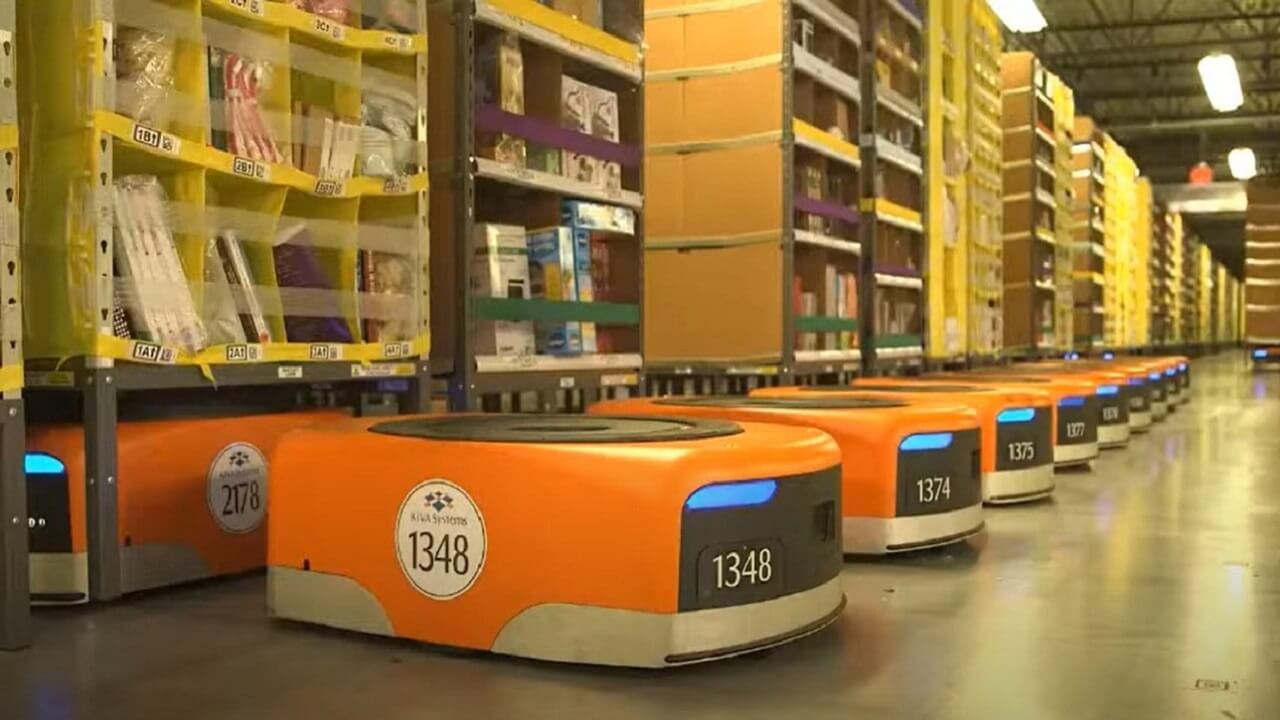
\includegraphics[width=\textwidth]{figures/chapter_intro/amazon_kiva.jpg}
    \caption{Amazon Kiva Robot}
    \label{fig:kiva}
\end{subfigure}
\hfill
\begin{subfigure}[b]{0.485\textwidth}
    \centering
    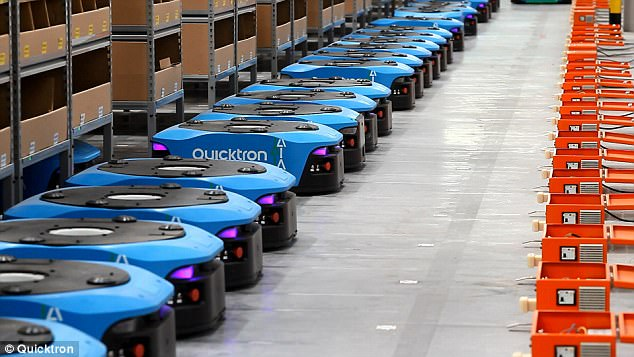
\includegraphics[width=\textwidth]{figures/chapter_intro/alibaba_quicktron.jpg}
    \caption{Alibaba Quicktron Robot}
    \label{fig:quicktron}
\end{subfigure}
\hfill
\caption{Robots in warehouse.}
\label{fig.robot}
\end{figure}

For instance, the Amazon Kiva Robot and Alibaba Quicktron Robot can help warehouse staffs find desired items by moving goods shelves. Each robot can perceive the surrounding environment to avoid collisions with other robots, and receive commands from warehouse staff via cloud servers. On the other hand, autonomous driving research teams from Waymo (formerly the Google self-driving car project), Tesla, etc intend to achieve autonomous navigation without human interference.

\begin{figure}[H]
\centering
\begin{subfigure}[b]{0.485\textwidth}
    \centering
    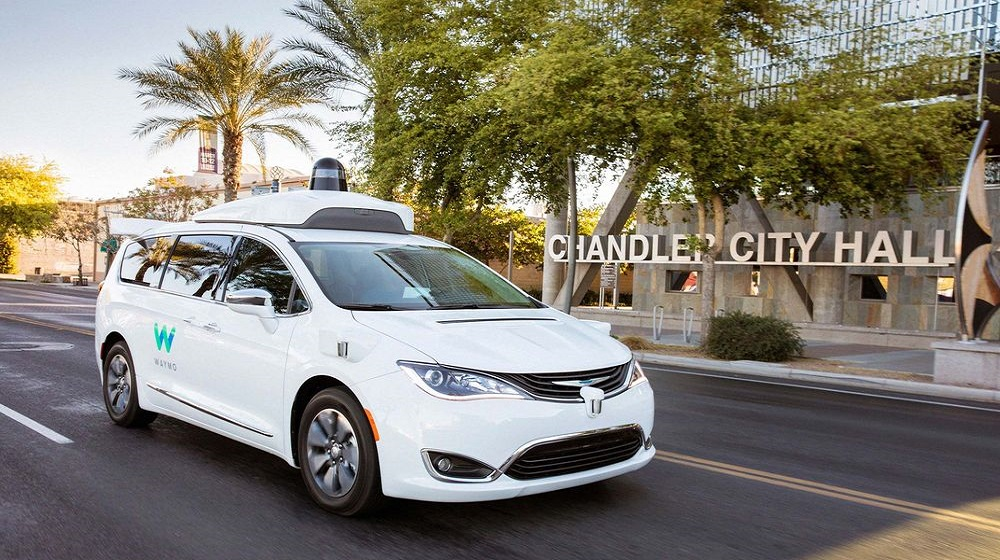
\includegraphics[width=\textwidth]{figures/chapter_intro/waymo.jpg}
    \caption{Waymo (formerly Google self-driving project)}
    \label{fig:waymo}
\end{subfigure}
\hfill
\begin{subfigure}[b]{0.485\textwidth}
    \centering
    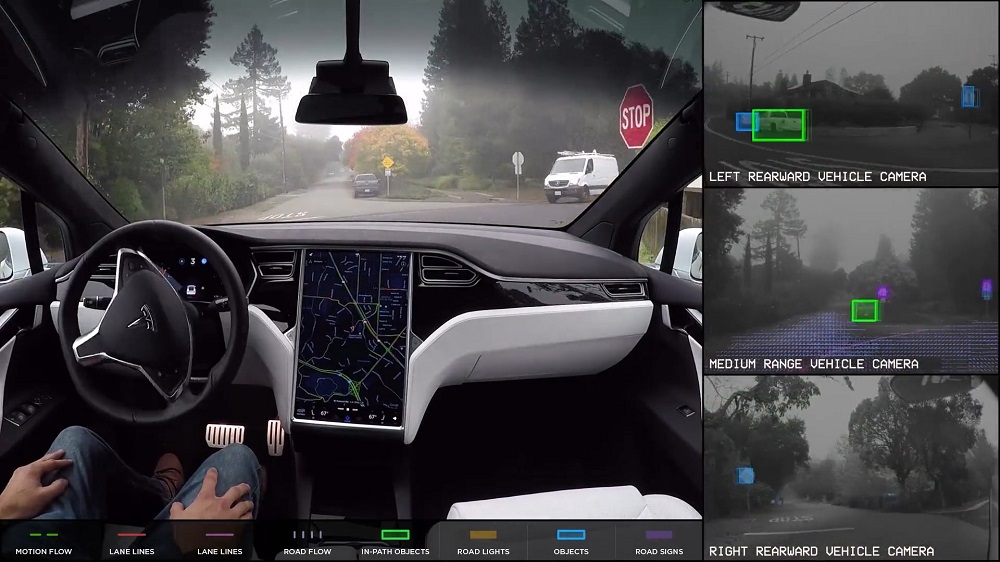
\includegraphics[width=\textwidth]{figures/chapter_intro/tesla_autopilot.jpg}
    \caption{Tesla Autopilot}
    \label{fig:tesla}
\end{subfigure}
\hfill
\caption{Autonomous Driving Research}
\label{fig.autonomous}
\end{figure}

Autonomous driving systems are commonly divided into sub-tasks: localization, perception, prediction, planning, and control. The vehicle determines its position in the environment through localization. Perception enables vehicles to collect information and extract relevant knowledge from the environment. The task of prediction makes predictions of measurement, behavior, trajectory, etc. The planning task makes purposeful decisions to achieve the goal, and the control component executes the planned actions \citep{pendleton2017perception}. Recently, the end-to-end driving that maps inputs directly to steering commands started to rise as an alternative to modular systems.

Our research focuses on adversarial attacks against deep learning models for mobile robots perception, such as image classification, object detection and object tracking in autonomous driving. We also investigate possible vulnerabilities in deep reinforcement learning.


\subsection{Deep Learning}
\label{sec:deep_robot}

As the research in deep neural networks advances, deep convolutional networks become feasible for automated driving tasks. Our research investigates the effect of adversarial attacks against deep learning models. However, it is risky to perform attacks against real-world autonomous driving systems. Thus adversarial attacks are tested in various simulators.

\begin{figure}[H]
\centering
\begin{subfigure}[b]{0.485\textwidth}
    \centering
    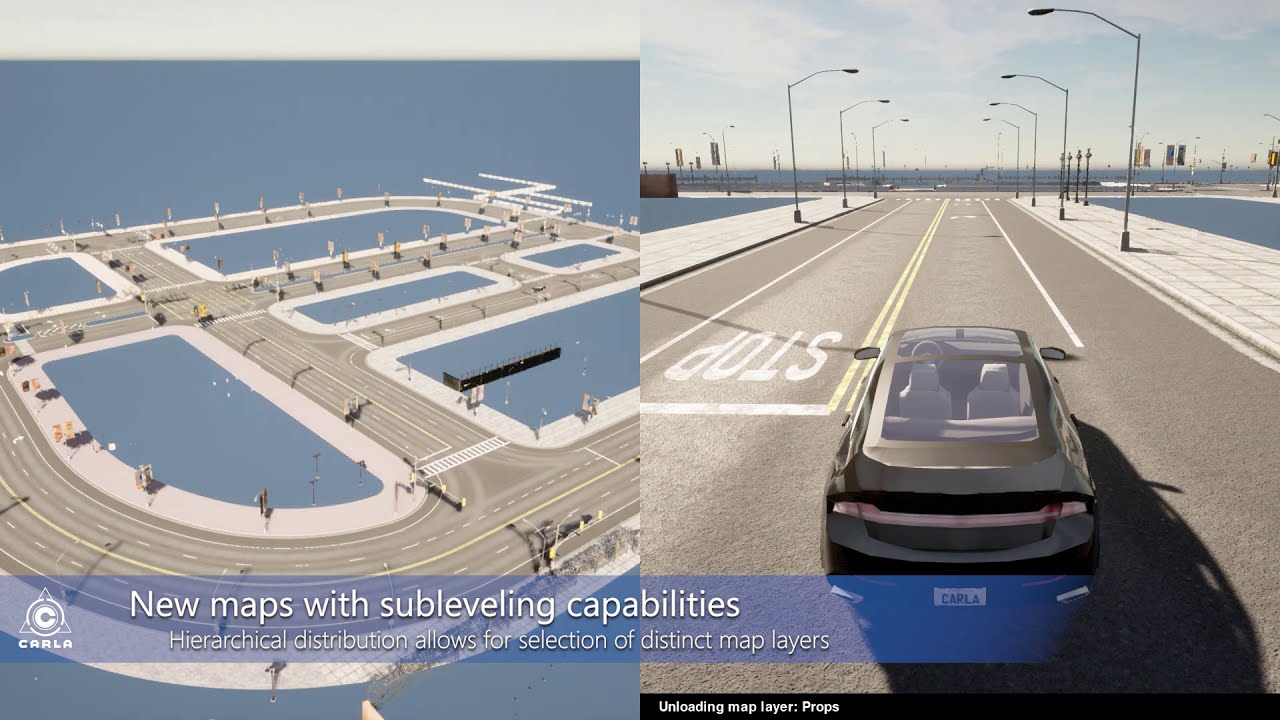
\includegraphics[width=\textwidth]{figures/chapter_intro/carla.jpg}
    \caption{Carla}
    \label{fig:carla_intro}
\end{subfigure}
\hfill
\begin{subfigure}[b]{0.485\textwidth}
    \centering
    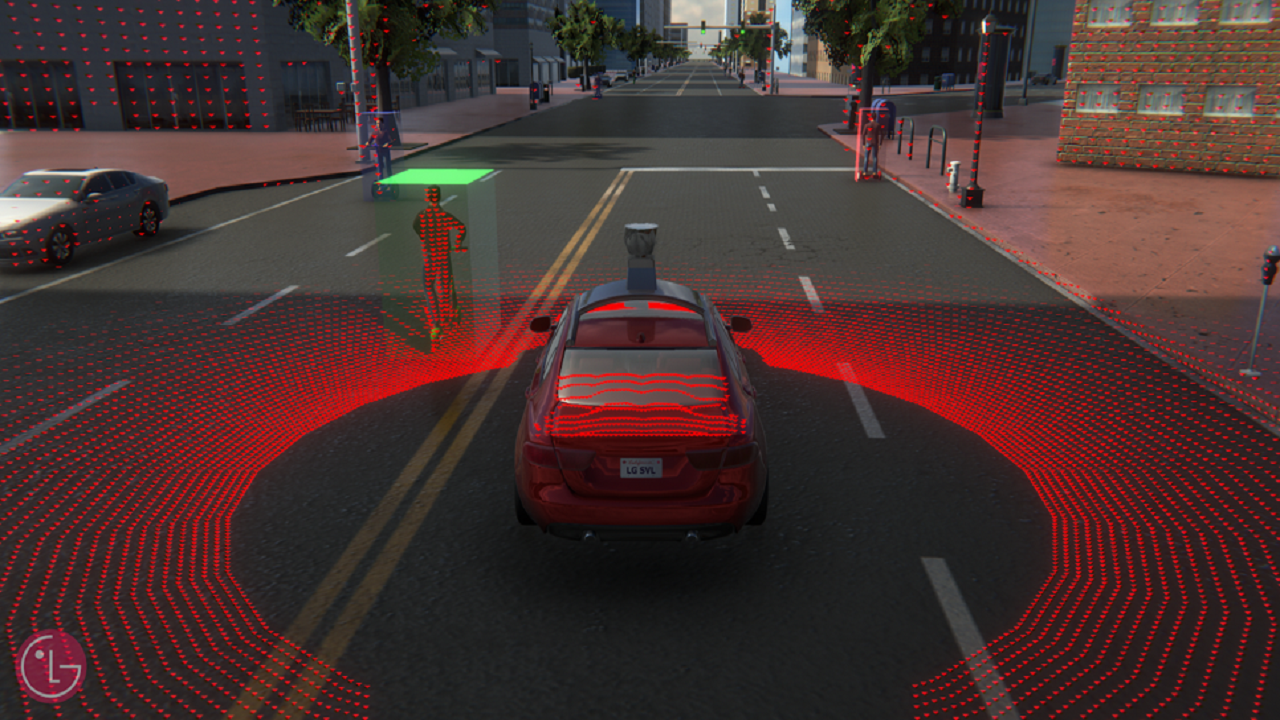
\includegraphics[width=\textwidth]{figures/chapter_intro/lgsvl.png}
    \caption{LGSVL}
    \label{fig:lvsvl}
\end{subfigure}
\hfill
\caption{Autonomous Driving Simulators}
\label{fig.simulator}
\end{figure}

The Carla simulator is an open-source platform for autonomous driving simulation based on the Unreal Game Engine. It simulates various sensors such as depth camera, 3D lidar, radar. The Carla simulator provides flexible Python API to manipulate the virtual environments and supports Robot Operating System (ROS) integration as well \citep{Dosovitskiy17}.

The LGSVL is another autonomous vehicle simulation platform based on the Unity3D Game Engine. It provides integration with the Baidu Apollo Platform \citep{rong2020lgsvl}. Besides, the Microsoft Airsim simulator provides virtual environments for both autonomous driving and drone simulation \citep{airsim2017fsr}.

\begin{figure}[H]
\centering
\begin{subfigure}[b]{0.485\textwidth}
    \centering
    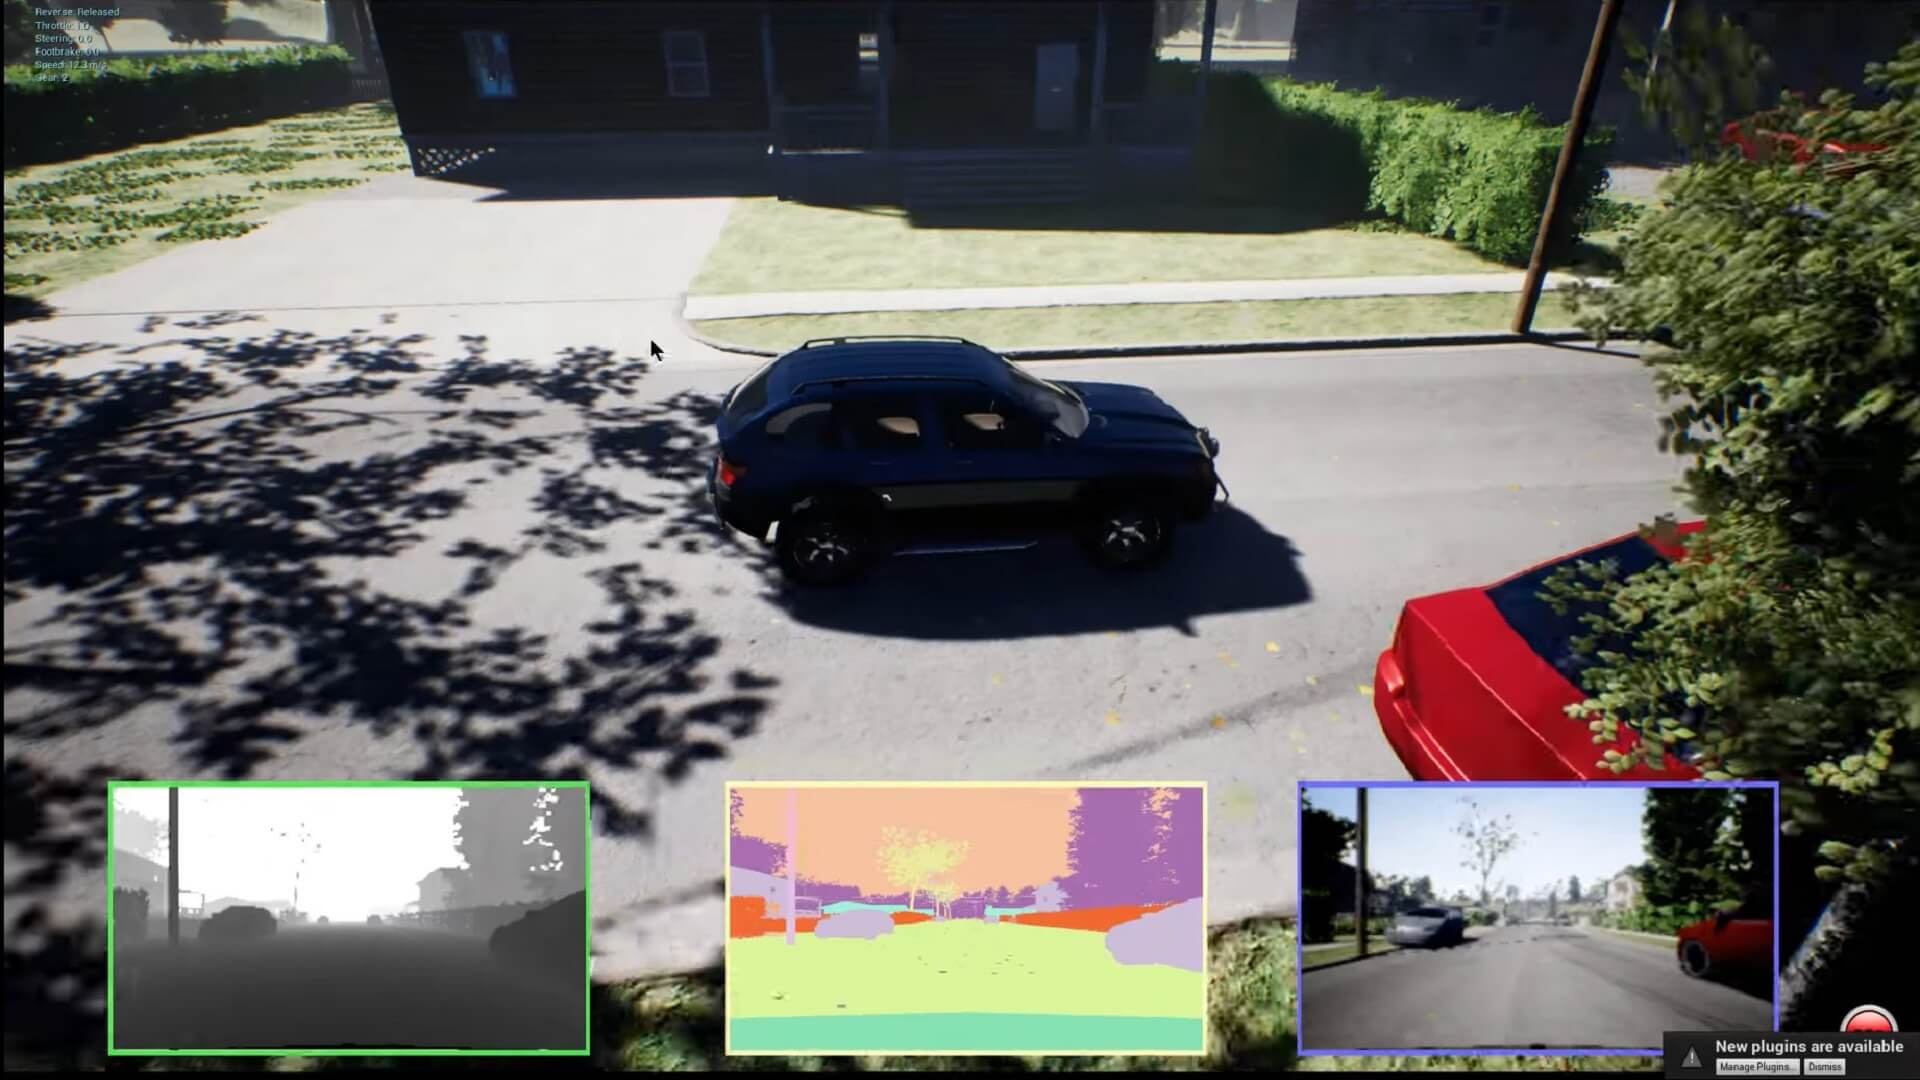
\includegraphics[width=\textwidth]{figures/chapter_intro/airsim_car.jpg}
    \caption{Airsim for Autonomous Driving}
    \label{fig:airsim_car}
\end{subfigure}
\hfill
\begin{subfigure}[b]{0.485\textwidth}
    \centering
    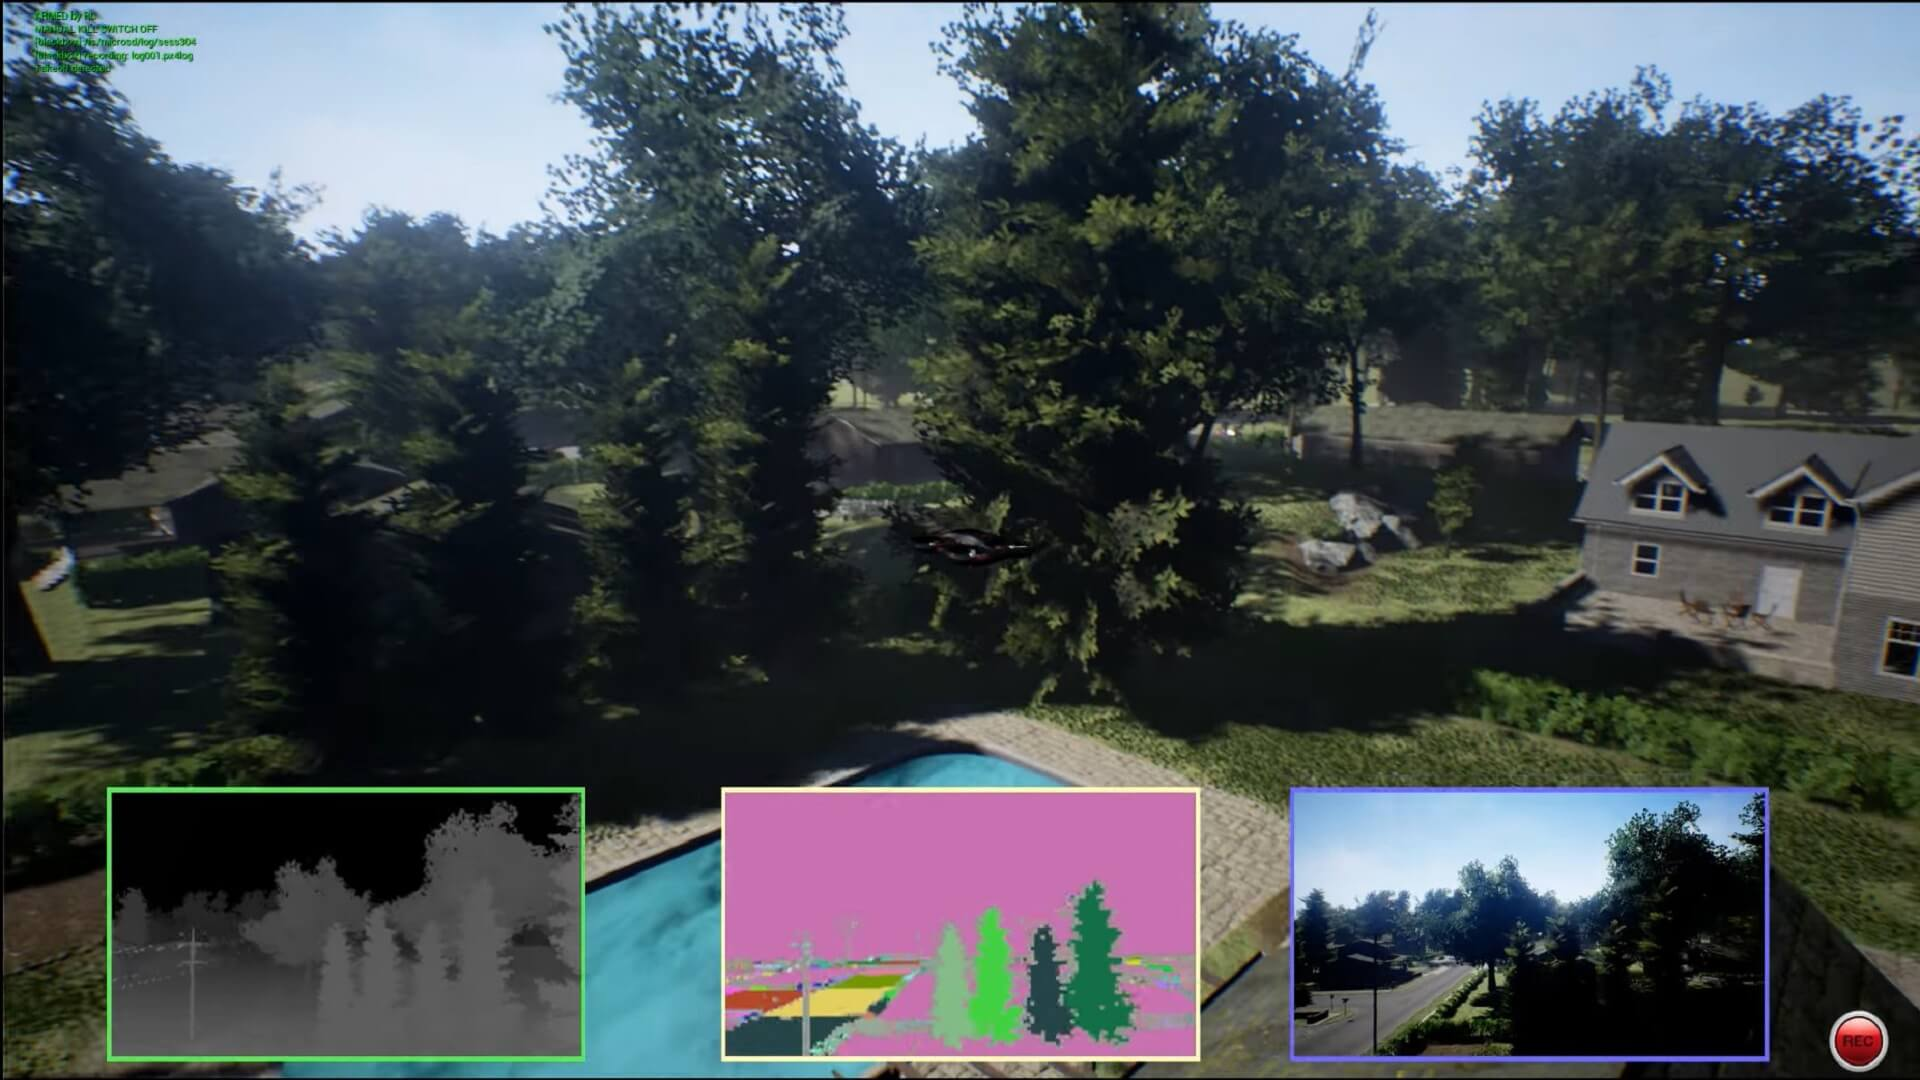
\includegraphics[width=\textwidth]{figures/chapter_intro/airsim_drone.jpg}
    \caption{Airsim for drones}
    \label{fig:airsim_drone}
\end{subfigure}
\hfill
\caption{Microsoft Airsim Simulator}
\label{fig.airsim}
\end{figure}

Practical adversarial attacks are introduced in the following three chapters. In chapter \ref{chpt:classification}, we investigate distributed black-box attacks against image classification models. In chapter \ref{chpt:detection}, we achieve real-time white-box attacks against object detection models. In chapter \ref{chpt:tracking}, we intend to attack object tracking systems, and examine the effect of hardware acceleration on the robustness of deep learning models. 

% Since end-to-end deep learning models are computationally expensive, pruning and quantization are commonly used techniques to make large models feasible for embedded systems, but theses techniques could render deep learning models more vulnerable.

In chapter \ref{chpt:defence}, the interpretability of deep learning models and defense methods against adversarial attacks are explored to help robots embrace deep neural networks safely.

% \clearpage

\subsection{Reinforcement Learning}
\label{sec:reinf_robot}

Deep reinforcement learning can be integrated into robotic systems as well. Given observations of the environment under certain states, the agent (robot) takes actions to achieve objectives. Most reinforcement learning tasks are evaluated in games such as the Atari. Recently, the NVIDIA Issac Gym simulator makes large-scale reinforcement learning possible.

\begin{figure}[H]
\centering
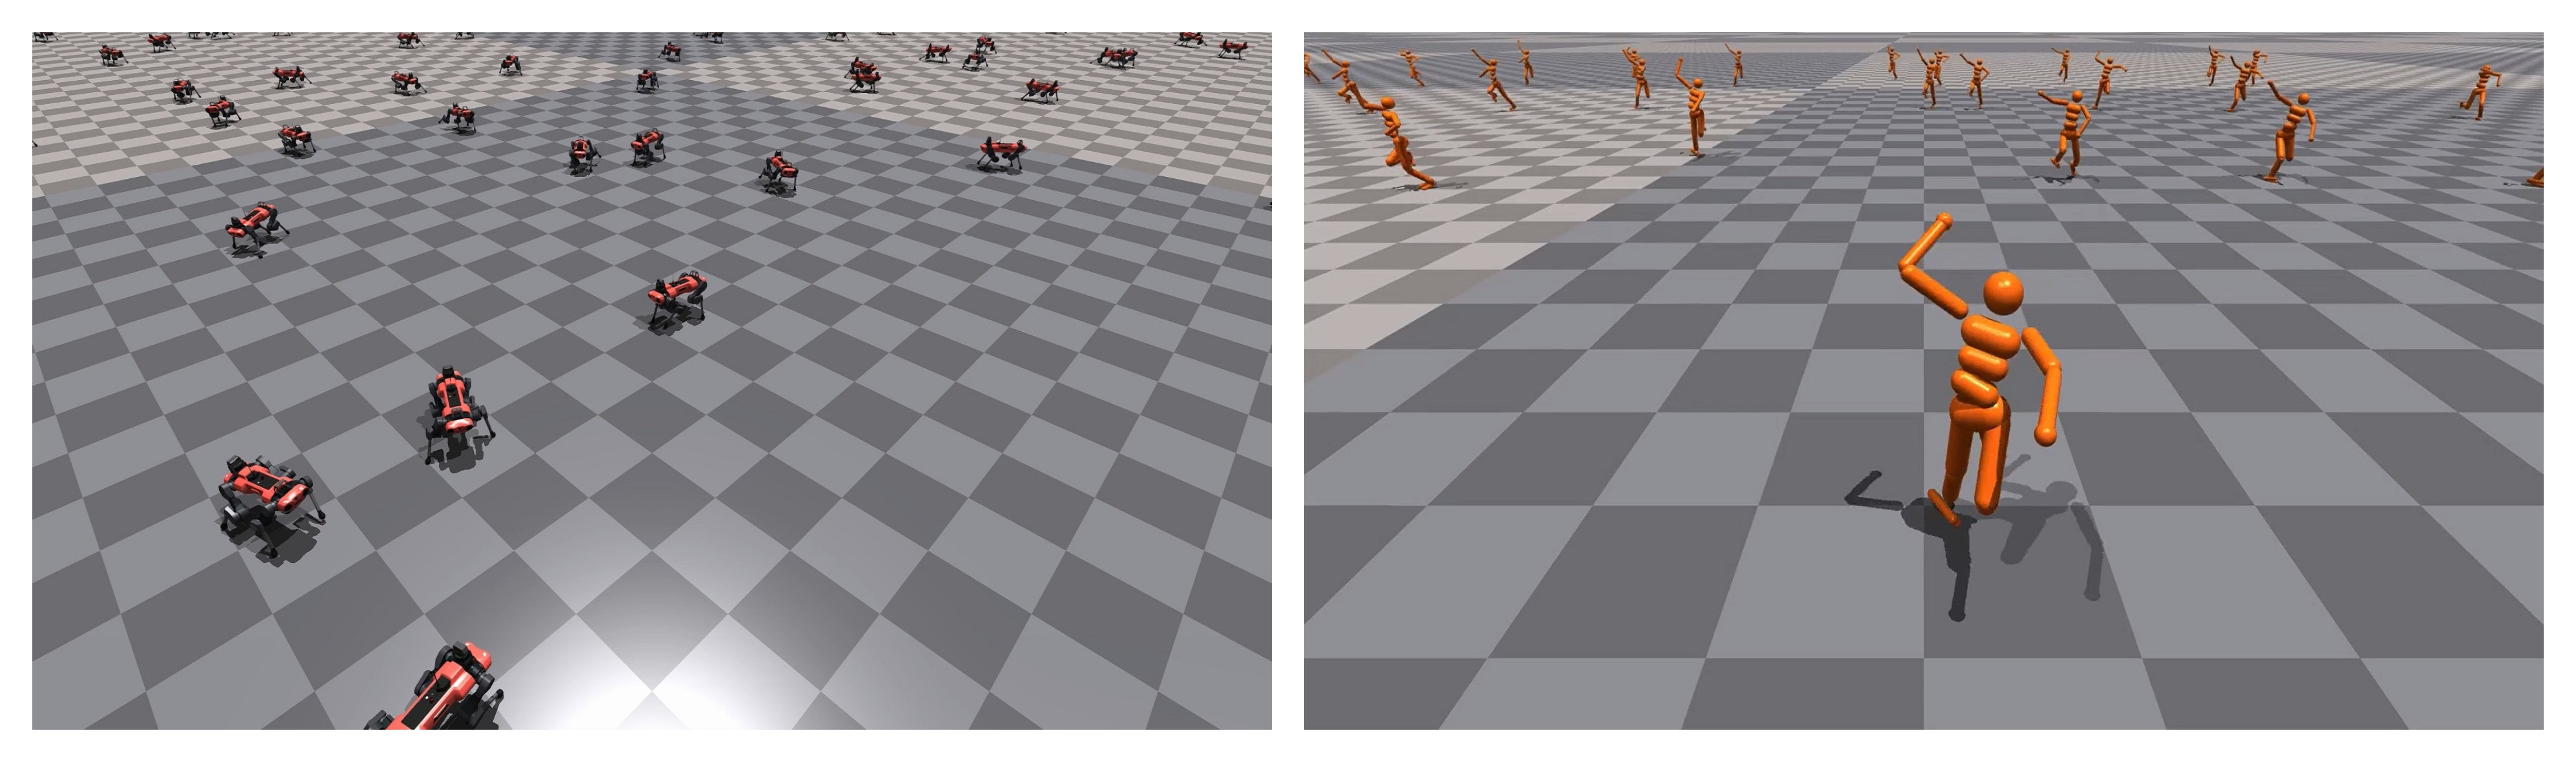
\includegraphics[width=\textwidth]{figures/chapter_intro/issac_gym.jpg}
\caption{NVIDIA Isaac Gym}
\label{fig.issac_gym}
\end{figure}

However, reinforcement learning models are vulnerable to adversarial attacks by adding perturbations to agents' observations \citep{chen2019adversarial}. Besides, recent research unveils that adversarial policy that acts abnormally in a shared environment can also induce extremely unlikely activations to occur.

\begin{figure}[H]
\centering
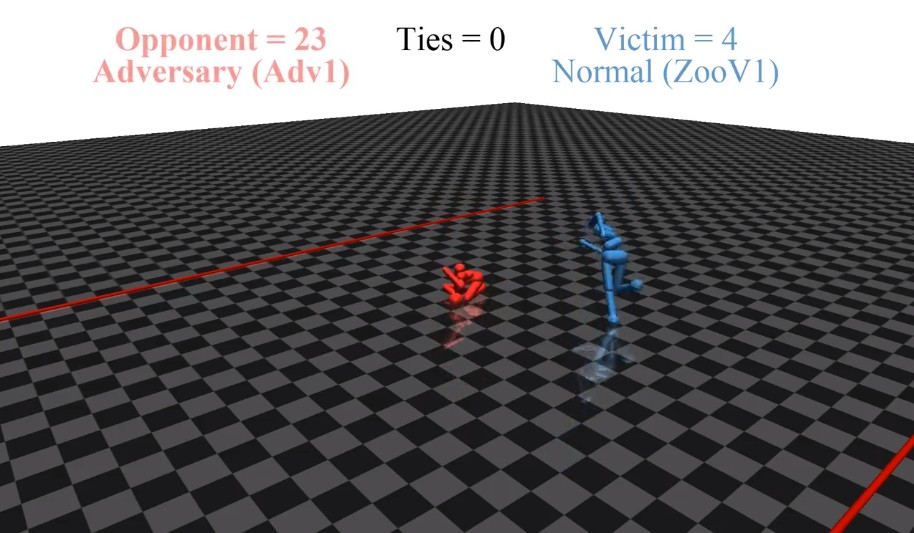
\includegraphics[scale=0.4]{figures/chapter_intro/adv_policy.jpg}
\caption{Adversarial Policies: Attacking Deep Reinforcement Learning}
\label{fig.adv_policy}
\end{figure}

For instance, the red agent tries to prevent the blue agent from crossing the line. Unexpectedly, the red agent wins the game by falling to the ground, which looks like a random policy. But this abnormal action of the red agent effectively causes the blue agent to fall as well \citep{gleave2021adversarial}. 

In chapter \ref{chpt:driving}, we provide more experiments of adversarial attacks against end-to-end models in autonomous driving systems.

\section{Adversarial Attacks}
\label{sec:adv_attack}

Existing adversarial attacks can be categorized into white-box, gray-box, and black-box attacks \citep{REN2020346}. In white-box attacks, the adversaries have full knowledge of the target model, including model architecture and parameters \citep{goodfellow2015explaining}. In gray-box attacks, the adversaries only have access to the structure of the target model. In black-box attacks, the adversaries can only gather information about the model through querying. In our research, we majorly focus on white-box and black-box attacks.

Depending on the goal of the attack, adversarial attacks can be further categorized into three types, evasion, poisoning, and extraction attacks \citep{art2018}. Evasion attacks cause models to make incorrect predictions by adding perturbations to the input during inference. The poisoning attack injects malicious data into the training set. Lastly, the extraction attack steals or replicates models that are available to query. For autonomous systems, rather than trying to steal models or poison others' training data, we intend to design a system that is resistant to malicious perturbations in the input. Thus our research object coincides with evasion attacks.

\subsection{White-Box Attacks}
\label{sec:whitebox_attack}

Deep learning models are trained by minimizing the loss function via updating weights according to gradients, while white-box attacks maximize the loss function by adding noises to the input.

\begin{figure}[H]
\centering
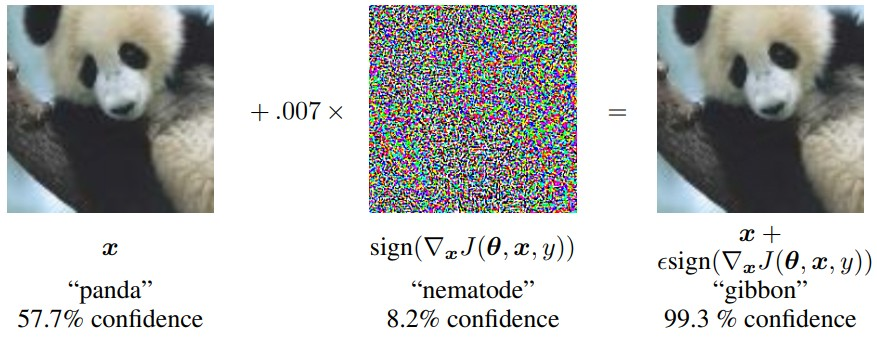
\includegraphics[scale=0.5]{figures/chapter_intro/fgsm.jpg}
\caption{Unperceivable perturbations on the full image}
\label{fig.adv_perturb}
\end{figure}

White-box attacks rely on gradients to fool deep learning models. Difference attack methods use different strategies to update the input using gradients. We can either generate human-unperceivable perturbations on the full image or a human-perceivable patch on a part of the image.

Most existing research on adversarial attacks choose a classification model as the target. A neural network is denoted as $f(\cdot)$ with input $x$ and prediction $f(x)$. The corresponding optimization loss is denoted by $J(\theta, x, y)$, where $\theta$ represents the model weights. An adversarial input $x'$ is close to the original input $x$ under a specific distance metric while $f(x') \neq f(x)$ \citep{REN2020346}. Formally, an adversarial sample of  is defined as follows:

$$x': D(x, x') < \eta, f(x') \neq y $$

Where $D(\cdot, \cdot)$ is the distance metric and $ \eta $ is a predefined distance constraint that defines the maximum allowed perturbation. The most commonly used distance metric is the $L_p$ distance metric. The distance between $x$ and $x'$ is denoted as $||x-x'||_{p}$, where $||\cdot||_p$ is defined as follows:

$$ ||v||_p = (|v_1|^p + |v_2|^p + \dots + |v_d|^p)^{1/p} $$

Where $p$ is a real number; $d$ is the dimension of the distance vector $v$. For instance, the $L_0$ distance corresponds to the number of pixels being modified in the perturbation. The $L_2$ distance measures the standard Euclidean distance between $x$ and $x'$. The $L_\infty$ distance measures the maximum element-wise difference between $x$ and $x'$.

The Fast Gradient Sign Method (FGSM) \citep{goodfellow2015explaining} generates the adversarial input by:

$$ x' = x + \epsilon \cdot sign(\bigtriangledown_x J(\theta, x, y)) $$

The Projected Gradient Descent (PGD) \citep{madry2017towards} method transforms the FGSM into a multi-step attack that takes only a small step at each iteration while keeping the perturbation in a $L_p$ ball:

$$ x^{t+1} = proj_{L_p}(x^t + \alpha \cdot sign(\bigtriangledown_x J(\theta, x, y))) $$

The Deep Fool \citep{moosavidezfooli2016deepfool} adds the norm of the gradient difference while iterating over each class:

$$ x^{t+1} = x^t + \frac{|f'_{\hat{l}}|}{||\omega'||^2_2} sign(\omega'_{\hat{l}})$$

If we further project the perturbation to $L_p$ ball of radius $\xi$ and centered at 0, we have the Universal Adversarial Perturbation \citep{moosavidezfooli2017universal}:

$$\mathcal{P}_{p, \xi}(v) = \arg\ \underset{v'}{\min}||v-v'||_2\ subject\ to\ ||v'||_p\leq\xi$$

% C\&W JSMA

The aforementioned methods intend to generate small perturbations to the entire image while keeping the perturbation small enough to be unnoticeable by human eyes. Under certain scenarios, if we opt for more effective but noticeable perturbation, we can generate an adversarial patch.

\begin{figure}[H]
\centering
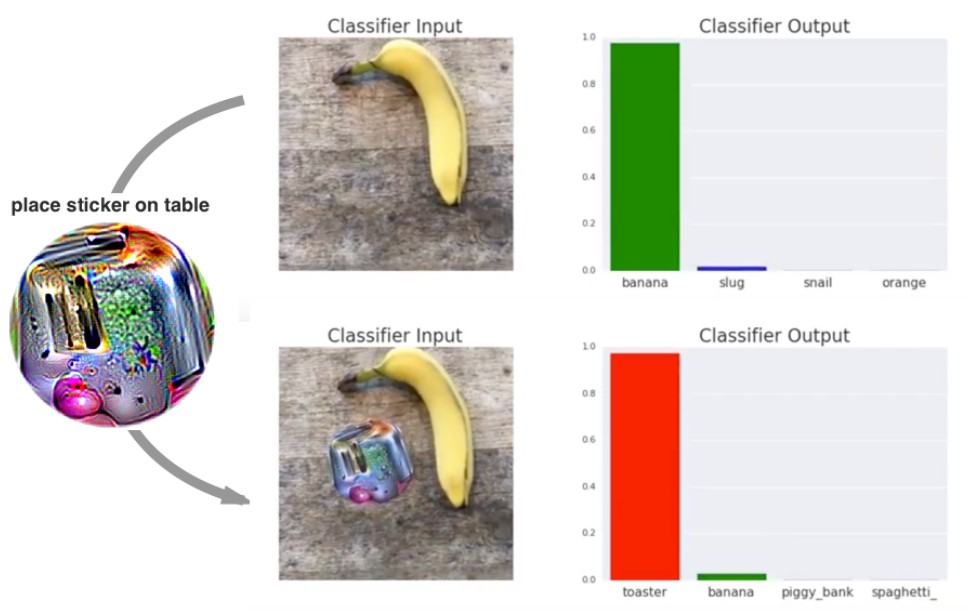
\includegraphics[scale=0.5]{figures/chapter_intro/adv_patch.jpg}
\caption{Perceivable perturbations as a patch}
\label{fig.adv_patch}
\end{figure}

A variant of the Expectation over Transformation (EOT) framework \citep{athalye2018synthesizing} is used to obtain the trained patch. In particular, the patch is trained to optimize the objective function:

$$\hat{p} = \arg \underset{p}{\max}\mathbf{E}_{x \sim X, t \sim T,l \sim L}[logPr(\hat{y}|A(p,x,l,t))]$$

where $X$ is a training set of images, $T$ is a distribution over transformations of the patch, and $L$ is a distribution over locations in the image \citep{brown2018adversarial}.

To design a printable physical patch, Non-Printability Score (NPS) can be used for measuring the error between a printed pixel and its digital counterparts. Sum of NPSs of all pixels in an image can be used to measure the image printability \citep{wang2021daedalus}.

$$\hat{p} = \arg \underset{p}{\min}\mathbf{E}_{x \sim X}\mathbf{E}_\phi f_3(x, p, \Phi) + SNPS(p, \beta)$$

where SNPS is the Sub-sampled Non-Printability Score of the poster $p$.

In chapter \ref{chpt:driving}, we introduce real-time white-box attacks against autonomous driving systems that that generate unnoticeable full-image perturbation.

In chapter \ref{chpt:detection}, we present real-time white-box attacks against object detection that generate noticeable adversarial patches.

% \clearpage

\subsection{Black-Box Attacks}
\label{sec:blackbox_attack}

White-box attacks that rely on gradients can generate adversarial inputs in real-time. However, gradients are not computed in real-world deep learning applications because those applications only perform the inference that does not require gradients. Without access to gradients, white-box attacks become infeasible in the real world.

Without access to gradients, black-box attacks generate adversarial inputs via querying. The Zeroth Order Optimization (ZOO) Attack amends the C\&W white-box attacks to the black-box setting by modifying the loss function and computing an approximate gradient using a finite difference method \citep{Chen_2017}.

$$f(x,t) = \max \{ {\underset{i \neq t}{\max}\ log[F(x)]_i - log[F(x)]_t, -\kappa } \}$$

The ZOO Attack relies on the output of confidence scores to estimate the gradient, while decision-based attacks can generate adversarial inputs using even less information.

\begin{figure}[H]
\centering
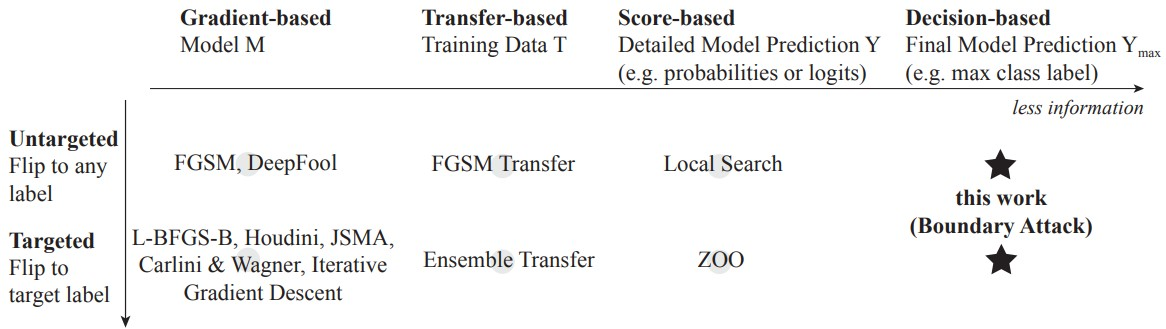
\includegraphics[scale=0.45]{figures/chapter_intro/query-efficient.jpg}
\caption{Decision-based adversarial attacks \citep{brendel2018decisionbased}}
\label{fig.query}
\end{figure}

For image classification tasks, decision-based attacks only require access to the predicted class, while score-based attacks require the predicted probability of each class.

\begin{figure}[H]
\centering
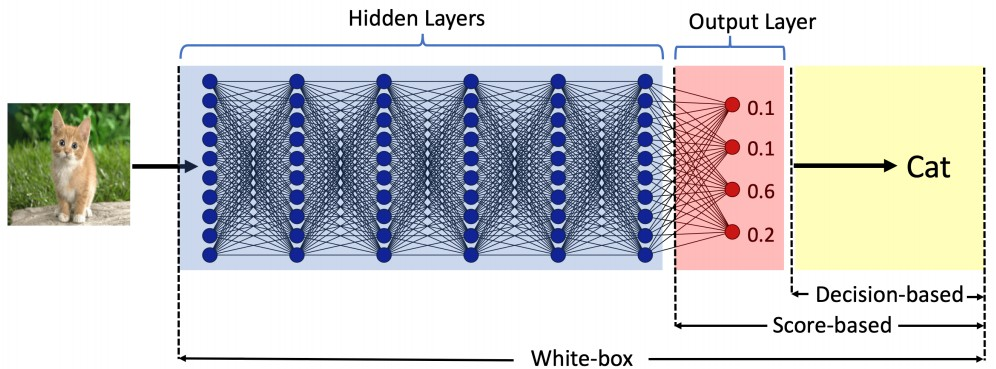
\includegraphics[scale=0.35]{figures/chapter_intro/score-decision.jpg}
\caption{The difference between score-based and decision-based attacks \citep{chen2020hopskipjumpattack}}
\label{fig.decision}
\end{figure}

In chapter \ref{chpt:classification}, we present adversarial classification, a black-box attack against cloud services of image classification.

\section{Research Questions}
\label{sec:research_question}

\section{Thesis Overview}

To achieve the research objectives set out in Section 1.4, the remaining of the thesis organized as follows:

Chapter 2: publication


%% LITERATURE REVIEW
\chapter{Adversarial Driving}
\label{chpt:driving}

% \newrefsection

As research in deep neural networks advances, deep convolutional networks become promising for autonomous driving tasks. In particular, there is an emerging trend of employing end-to-end neural network models for autonomous driving. However, previous research has shown that deep neural network classifiers are vulnerable to adversarial attacks. While for regression tasks, the effect of adversarial attacks is not as well understood. In this chapter, we devise two white-box targeted attacks against end-to-end autonomous driving models. Our attacks manipulate the behavior of the autonomous driving system by perturbing the input image. In an average of 800 attacks with the same attack strength (epsilon=1), the image-specific and image-agnostic attack deviates the steering angle from the original output by 0.478 and 0.111, respectively, which is much stronger than random noises that only perturbs the steering angle by 0.002 (The steering angle ranges from [-1, 1]). Both attacks can be initiated in real-time on CPUs without employing GPUs. 

% Demo video: \href{https://youtu.be/I0i8uN2oOP0}{https://youtu.be/I0i8uN2oOP0}.

% The driving system uses a regression model that takes an image as input and outputs the steering angle. 

\section{Introduction}

Autonomous driving is one of the most challenging tasks in safety-critical robotic applications. Most real-world autonomous vehicles employ modular systems that divide the driving task into smaller subtasks. In addition to a perception module that relies on deep learning models to locate and classify objects in the environment, modular systems also include localization, prediction, planning, and control modules. However, researchers are also exploring the potential of end-to-end driving systems. An end-to-end driving system is a monolithic module that directly maps the input to the output, often using deep neural networks. For example, the NVIDIA end-to-end driving model \citep{bojarski2016end} maps raw pixels from the front-facing camera to steering commands. The development of end-to-end driving systems has been facilitated by recent advances in high-performance GPUs and the development of photo-realistic driving simulators, such as the Carla Simulator \citep{Dosovitskiy17} and the Microsoft Airsim Simulator \citep{airsim2017fsr}.  

\begin{figure}[H]
    \centering
    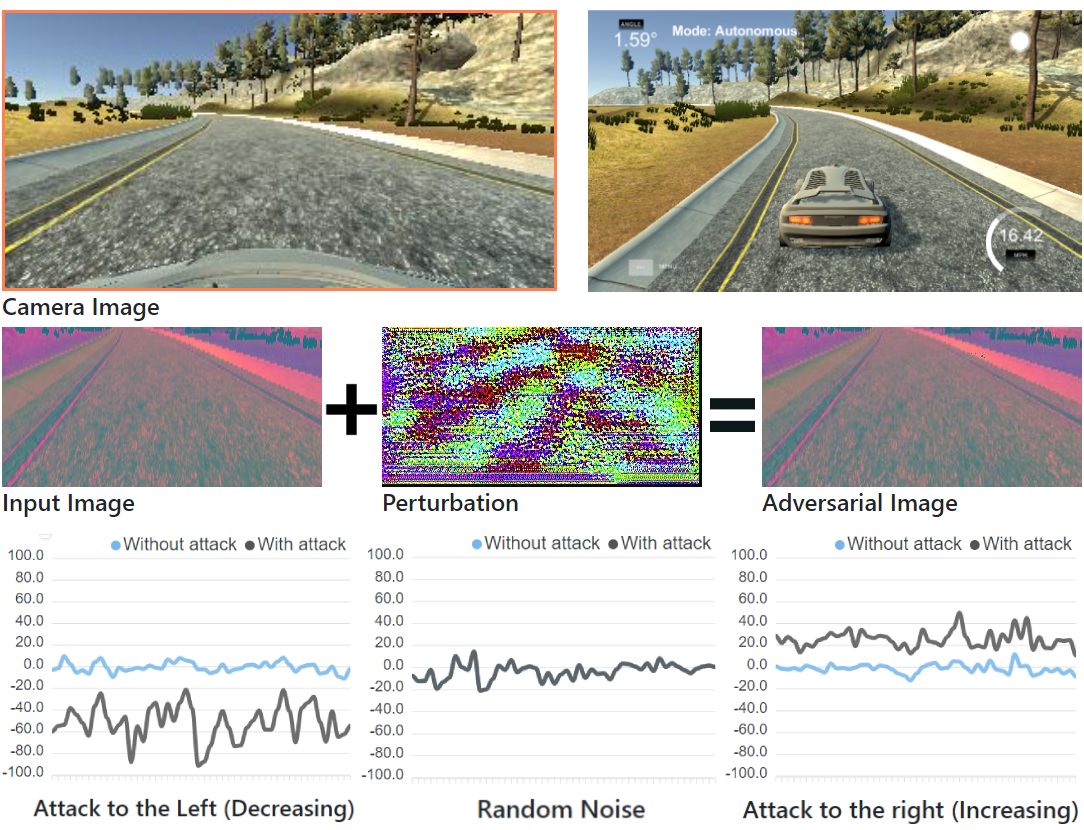
\includegraphics[width=\textwidth]{figures/chapter_driving/overview.png}
    \caption{Adversarial Driving: The behavior of and end-to-end autonomous driving model can be manipulated by adding unperceivable perturbations to the input image.}
    \label{fig:adv_drv}
\end{figure} 

As demonstrated in multiple contexts, deep neural networks are vulnerable to adversarial attacks. Typically, these attacks fool an image classification model by adding an unperceivable perturbation to the input image \citep{goodfellow2014explaining}. Despite the fact that the number of academic publications discussing end-to-end deep learning models is steadily increasing, their safety in real-world scenarios is still unclear. Though end-to-end models may lead to better performance and smaller systems, the monolithic module is also particularly vulnerable to adversarial attacks. In addition, note that current research on adversarial attacks primarily focuses on classification tasks. The effect of these attacks on regression tasks, however, largely remains unexplored. Our research explores the possibility of achieving real-time attacks against NVIDIA's end-to-end regression model (See Fig. \ref{fig:adv_drv}). However, the attacks may also be applied to the perception module in a modular driving system.


The main contributions of this chapter are as follows: 

\begin{itemize}
    \item We propose two online white-box adversarial attacks against an end-to-end regression model for autonomous driving: one strong attack that generates the perturbation for each frame (image-specific), and one stealth attack that produces a universal adversarial perturbation that attacks all frames (image-agnostic).
    \item The robustness of the attacks is illustrated using experiments conducted in Udacity Simulator. 
    The experiments demonstrate that it only takes the attack a few seconds to deviate the vehicle to outside of the lane.
    \item To facilitate future extensions and benchmark comparisons, our attack is open-sourced on Github\footnote{The code is available on Github: \url{https://github.com/wuhanstudio/adversarial-driving}}. As far as the authors are aware, this is the first open-source real-time attack on regressional driving models.
\end{itemize}

% \clearpage

\section{Preliminaries}

% Modular System

This section categorizes and describes end-to-end driving systems and associated adversarial attacks.

\subsection{End-to-End Driving Systems}

%Recent advances in autonomous driving simulators stimulate the development of end-to-end driving systems. Modular systems divide the driving pipeline into submodules and employ end-to-end models in the perception module. On the other hand, end-to-end driving systems treat the entire driving pipeline as a monolithic module that maps sensor inputs directly to steering commands \citep{Yurtsever2020}.

End-to-end driving systems treat the driving pipeline as a monolithic module that maps sensor inputs directly to steering commands \citep{Yurtsever2020}. Typically, end-to-end driving systems are implemented using either imitation learning or reinforcement learning. Imitation learning methods use deep neural networks to learn and mimic human driving behavior \citep{chen2022learning}. A supervisor is responsible for feeding the algorithm with labeled data. Reinforcement learning methods, on the other hand, improve driving policies via exploration and exploitation. The training process is not dependent on the existence of any supervisor. While there is a growing trend of publications that use reinforcement learning \citep{Chopra2020}\citep{perez2022deep}\citep{1286725}\citep{jaafra2019seeking}\citep{Chitta2021ICCV}, imitation learning is still more popular in end-to-end driving models \citep{tampuu2020survey}\citep{Prakash2021CVPR}\citep{Chitta2022PAMI}\citep{wu2022trajectory}. For this reason, our research will also focus on attacking imitation learning models.

The first implementation of an imitation-learning-based end-to-end driving system was the Autonomous Land Vehicle in a Neural Network (ALVINN) system, which trained a 3-layer fully connected network to steer a vehicle on public roads \citep{NIPS1988_812b4ba2}. However, end-to-end driving models have also been applied for the task of off-road driving \citep{NIPS2005_fdf1bc56}. More recently, researchers from NVIDIA built a convolutional neural network to map raw pixels from a single front-facing camera directly to steering commands \citep{bojarski2016end}. The NVIDIA end-to-end driving model is the target model in this paper, and details on this model are presented in Section \ref{section_problem_formulation}.

\subsection{Adversarial Attacks}
\label{adversarial_attacks}

This paper will consider an end-to-end driving model that outputs continuous steering commands, which is a regression model. Prior research on adversarial attacks primarily focuses on attacking classification models \citep{li2022review} \citep{zhang2021evaluating}\citep{boloor2019simple}\citep{abideen2022a3d}.

A successful attack against classification models deviates the output from the correct label. Taking the digital handwritten digit classification task as an example, an attacker can fool the classifier into recognizing the number 3 as 7. To evaluate the performance of an adversarial attack against a regression model, we need to quantify the magnitude of the resulting deviation. An attack that causes the steering angle to deviate from 1.00 to 0.99 will typically be considered unsuccessful since such a tiny deviation may not have any noticeable effect on the driving outcome. To be considered successful, an attack must lead to larger deviations. Prior research used Root Mean Squared Error (RMSE) \citep{msml} and Mean Square Error (MSE) \citep{nguyen2018adversarial} to evaluate and compare deviations. A successful attack should produce a higher MSE or RMSE than random attacks. Boloor et al. attacked an end-to-end self-driving model using human-perceivable physical shadow \citep{boloor2019}, while our research focuses on generating human-unperceivable perturbations.

While prior research primarily focuses on offline attacks against classification models, we investigate online attacks against regression models. Offline attacks apply perturbations to static images. Under the scenario of autonomous driving, an offline attack splits the driving record into static images and the corresponding steering angles. The perturbation is then applied to each static image, and the attack is evaluated using the overall success rate \citep{Deng2020}. Online attacks, on the other hand, apply the perturbation in a dynamic environment. Rather than applying the perturbation to static images in a driving record, we deploy the perturbation while the vehicle is driving. This also makes it possible to investigate the driving models' reactions to the attacks. 

One big difference between online and offline attacks is that the ground truth is unavailable in online attacks. Offline attacks take pre-recorded human drivers' steering angles as the ground truth, while real-time online attacks do not have access to pre-recorded human decisions. Therefore, we use the model output under normal benign conditions as the ground truth and assume that the driving model is comparatively close to the ground truth. This assumption is reasonable since if the model is inaccurate, the erroneous model is already a threat in itself. There is no need to attack the system in the first place.

Existing adversarial attacks can be categorized into white-box, gray-box, and black-box attacks \citep{REN2020346}: In white-box attacks, the adversaries have full knowledge of the target model, including model architecture and parameters; In gray-box attacks, the adversaries have partial information about the target model; In black-box attacks, the adversaries can only gather information about the model through querying. Since white-box attacks are more efficient, we devise two white-box attacks that achieve real-time performance against end-to-end driving models .

% \clearpage

\section{Problem Formulation}
\label{section_problem_formulation}

In this section, we specify our objective, introduce mathematical notation, and describe our target model. Throughout the paper, we will use the notation
\begin{align}
y&=f(\theta, x) \\
y'&=f(\theta, x')
\end{align}
where $y$ is the benign output steering command, $f(\theta, x)$ is the regression model that maps input images to steering commands, $\theta$ is the model parameters, $x$ is the original input image, $y'$ is the adversarial output steering command, and $x'$ is the adversarial input image. Further, we will use $\eta=x-x'$ to denote the adversarial perturbation, $y^{*}$ is the ground truth steering command, and $\mathcal{L}(y, y^{*})$ to denote the training loss. Given an input image $x$, the objective of attacking a classifier is to generate a small perturbation $\eta$, such that $y' \neq y^{*}$. However, the objective of attacking a regression model is to generate a small perturbation $\eta$, such that the difference between $y'$ and $y^{*}$ is larger than the average deviation caused by adding random noise to $x$. 

We use the $L_2$ norm to quantify the magnitude of the perturbation. The $L_2$ norm of the perturbation $\eta$ should be smaller than 0.03 (8 / 255) for an RGB input image according to the value used in prior research \citep{chow2020adversarial} \citep{ACFH2020square}. In particular, to ensure that the perturbation is unperceivable to human eyes, we require \begin{equation}
||x^{'}-x||_{2} = ||\ {\eta}\ ||_{2} \leq \xi %,\ \xi = 0.03
\end{equation}
where $\xi = 0.03$.

Our target model is the NVIDIA end-to-end driving model \citep{bojarski2016end}. The input shape of the model is (160, 320, 3), which represents (height, width, channel) respectively. The output steering angle is in the range of $[-1, 1]$ on all our (unperturbed) collected images. An output of $-1$ represents steering to the left, and an output of 1 means steering to the right. The input image is captured by the front camera, and we then apply predefined preprocessing methods before feeding the image to the model. Refer to \citep{bojarski2016end} for details on these preprocessing methods, including cropping, resizing, and RGB to YUV. 

% The structure of the driving model is detailed in Table \ref{table_NVIDIA_model}.

% \begin{table}[H]
% \begin{center}
% \begin{tabular}{ c c c }
%      \hline
%      Layer & Output Shape & Parameters \\ 
%      \hline
%      Input & (None, 160, 320, 3) & 0 \\  
%      Conv2D & (None, 78, 158, 24) & 1824 \\  
%      Conv2D & (None, 37, 77, 36) & 21636 \\  
%      Conv2D & (None, 17, 37, 48) & 43248 \\  
%      Conv2D & (None, 15, 35, 64) & 27712 \\  
%      Conv2D & (None, 13, 13, 24) & 36928 \\
%      Dropout & (None, 13, 13, 24) & 0 \\
%      Flatten & (None, 27456) & 0 \\
%      Dense & (None, 100) & 2745700 \\
%      Dense & (None, 50) & 5050 \\
%      Dense & (None, 10) & 510 \\
%      Dense & (None, 1) & 11 \\
%      \hline
%     \end{tabular}
%     \caption{The structure of the end-to-end driving model. \label{table_NVIDIA_model}}
% \end{center}
% \end{table}

% Layer (type)                 Output Shape              Param #
% =================================================================
% Input             (None, 160, 320, 3)       0
% _________________________________________________________________
% Conv2D              (None, 78, 158, 24)       1824
% _________________________________________________________________
% Conv2D            (None, 37, 77, 36)        21636
% _________________________________________________________________
% Conv2D            (None, 17, 37, 48)        43248
% _________________________________________________________________
% Conv2D            (None, 15, 35, 64)        27712
% _________________________________________________________________
% Conv2D            (None, 13, 33, 64)        36928
% _________________________________________________________________
% Dropout            (None, 13, 33, 64)        0
% _________________________________________________________________
% Flatten            (None, 27456)             0
% _________________________________________________________________
% Dense                (None, 100)               2745700
% _________________________________________________________________
% Dense              (None, 50)                5050
% _________________________________________________________________
% Dense              (None, 10)                510
% _________________________________________________________________
% Dense              (None, 1)                 11
% =================================================================
% Total params: 2,882,619

\section{Adversarial Attacks} 

In this section, we devise two white-box attacks against the driving system: one image-specific attack and one image-agnostic attack, and the system architecture. 

% Then, we present the system architecture.

\subsection{The Image-specific Attack}

The first adversarial attack against a classifier was an image-specific offline attack that generated one perturbation for every input image \citep{goodfellow2014explaining}. Instead of minimizing the training loss $\mathcal{L}(y,\ y^{*})$, Goodfellow et al. maximized the training loss and then used the gradient of the training loss to generate the perturbation. However, online attacks do not have access to the ground truth $y^{*}$, and thus, for online attacks, the training loss $\mathcal{L}(y, y^{*})$ cannot be calculated. As a result, we need a new adversarial loss $\mathcal{L}(y)$ that only requires the model output $y$ to generate the perturbation.

When attacking a regression model, notice that we have the choice to either increase or decrease the output. For example, to attack the end-to-end driving regression model, we can either deviate the vehicle to the left by decreasing the output or to the right by increasing the output. Therefore, in some sense, attacks on regression models can be seen as a special case of attacks on classification models, with the constraint that we only have two choices: increasing or decreasing the output. Accordingly, we will consider the straightforward adversarial loss functions 
% \begin{equation}
% \eta=\epsilon \text{sign}(\nabla_{x}J(\theta, x, y)).
% \end{equation}

\begin{align}
    \mathcal{L}_{\texttt{left}}(y) &= -y \\
    \mathcal{L}_{\texttt{right}}(y) &= y
\end{align}
for the image-specific attack. 

As explained in Section \ref{adversarial_attacks}, the adversarial loss functions $\mathcal{L}(y)$ do not include ground truth $y^{*}$, which we do not have access to for online attacks. We can then utilize the Fast Gradient Sign Method (FGSM) to generate perturbations as 
\begin{equation}
    \eta = \epsilon \ \text{sign}[\nabla_{x}( \mathcal{L}(y))]
\end{equation}
where $\epsilon$ is a scaling factor that determines the visibility of the perturbation. The image-specific attack is summarized in Algorithm \ref{alg:image-specific-driving}.

\begin{algorithm}[H]
    \caption{Image-specific Attack}\label{alg:image-specific-driving}
    \begin{algorithmic}
        \State Input: The regression model $f(\theta, x)$, the input images $\{x_t\}$ where $x_t$ is the image at time step $t$.
        \State Parameters: The strength of the attack $\epsilon$.
        \State Output: Image-specific perturbation $\eta$.
        \For{each time step $t$}
            \State Inference: $y = f(\theta, x)$
            \State Perturbation: $\eta = \epsilon \ \text{sign}[\nabla_{x}( \mathcal{L}(y))]$
        \EndFor
    \end{algorithmic}
\end{algorithm}

As an example, assume that the attacker wishes to attack the vehicle to the right side. In this case, the objective is to increase the model output. We can then use the adversarial loss $J_{right}(y)$ to generate the perturbation. $\nabla_{x}( \mathcal{L}(y))$ represents the gradient of the adversarial loss over the input. The gradient gives us information regarding how changes in the adversarial loss $y$ will back-propagate to the input.

%Our experimental results show that the image-specific attack is a strong attack that deviates the vehicle to the outside of the lane in several seconds.

\begin{algorithm}[t]
    \caption{Image-agnostic Attack (Training)}\label{alg:image-agnostic-driving}
    \begin{algorithmic}
        \State Input: The regression model $f(\theta, x)$, input images in a driving record $X$, the target direction $I \in \{-1, 1\}$.
        \State Parameters: the number of iterations $n$, the learning rate $\alpha$, the step size $\xi$ , and the strength of the attack $\epsilon$ measured by the $l_{\infty}$ norm.
        \State Output: Image-agnostic perturbation $\eta$.

        \State Initialization: $\eta \leftarrow 0$
        \For{each iteration}
            \For{each input image $x$ in the driving record $X$}
                \State Inference: $y = f(\theta, x + \eta)$
                \If {$\text{sign}(y) \neq I$}
                    \State $x^{'} = x + \eta$
                    \State $\eta_{t} \leftarrow 0$
                    \While{$\text{sign}(y) \neq I$}
                        \State Gradients: $\nabla = \frac{\partial \mathcal{L}(y)}{\partial x'}$
                        \State Perturbation: $\eta_{t} = \eta_{t} + proj_{2}(\nabla,\ \xi)$
                        \State Inference: $y = f(\theta, x + \eta_t)$
                    \EndWhile
                    \State $\eta = proj_{\infty}(\eta + \frac{\alpha}{\xi} \eta_{t},\ \epsilon)$
                \EndIf
            \EndFor
        \EndFor
    \end{algorithmic}
\end{algorithm}

\subsection{The Image-agnostic Attack}

Even small deviations may cause traffic accidents. A small deviation in the steering angle may, for example, result in a failure to steer around a sharp corner. In other words, even if the attack is not as strong as the image-specific attack it could still be perilous if applied at critical time points. Therefore, we introduce a white-box attack that generates a universal adversarial perturbation (UAP) \citep{moosavi2017universal} which can be used to attack all input images at different time steps. The image-agnostic attack combines the idea of DeepFool \citep{moosavi2016deepfool} and Projected Gradient Descent (PGD) \citep{madry2017towards}. The attack consists of two procedures: training and deployment. We first generate a UAP online or via a driving record and then deploy the UAP.

We first decide our target direction, that is, whether to attack the vehicle to the left ($y < 0$) or to the right ($y > 0$), and then choose the corresponding adversarial loss function ($J_{\texttt{left}}(y)$ or $J_{\texttt{right}}(y)$). The perturbation is initialized as zero. For each input image at each timestep, if the direction of the model output is not the same as the desired direction, we find the minimum perturbation that changes the sign of the model output to the desired direction. 

To change the direction of the model output with the minimum perturbation, we calculate the gradient of the adversarial loss $\mathcal{L}(y)$ and then project the gradient to the $L_2$ ball. The closed-form solution to the optimization problem $\arg \min \ ||\ \eta - \eta^{'} \ ||_{2}$ with the constraint $||\ \eta^{'} \ || \leq \xi$ is given by
\begin{equation}
    proj_{2}(\eta,\  \xi) = \frac{\eta}{\max\{1, \frac{||\ \eta\ ||}{\xi}\}} =  \eta \min\{1, \frac{\xi}{||\ \eta\ ||} \}
\end{equation}
which can be proved using the Lagrangian and the KKT conditions \citep{boyd2004convex}.

% \begin{equation}
% \arg\underset{{\eta}^{'}}{\min }||\eta-\eta^{'}||_{2} \text{ subject to } ||{\eta}^{'}||_{2} \leq \xi
% \end{equation}

% \begin{equation}
% \Delta \eta_{t} = proj_{2}(\eta,  \xi) = \xi \frac{\nabla_{x} [J(y)]}{||\ \nabla_{x} [J(y)]\ ||_{2}}
% \end{equation}

After applying the temporary perturbation $\eta_{t}$ at timestep $t$, if the direction of the model output matches the desired direction, we incorporate the temporary perturbation $\eta_{t}$ to the overall perturbation $\eta$ and then project $\eta$ on the $l_2$ ball centred at 0 and of radius $\epsilon$ to ensure that the constraint $||{\eta}^{'}||_{2} \leq \epsilon$ is satisfied. The attack is summarized in Algorithm \ref{alg:image-agnostic-driving}. As can be seen, the attack uses a similar while loop as in DeepFool and the projection function introduced in the PGD attack.

%The strength of the attack is not as strong as the image-specific attack, but it still adds an opposite force to the vehicle while turning through the corner.

\subsection{System Architecture}

The Robot Operating System (ROS) \citep{ros} is the most popular software framework in robotic research and applications. One example of an attack that
injects malicious data into a running ROS application is the Stealth Publisher Attack \citep{dieber2020penetration}. We exploit the same vulnerability to inject adversarial perturbations into a running end-to-end driving ROS application.

\begin{figure}[H]
    \centering
    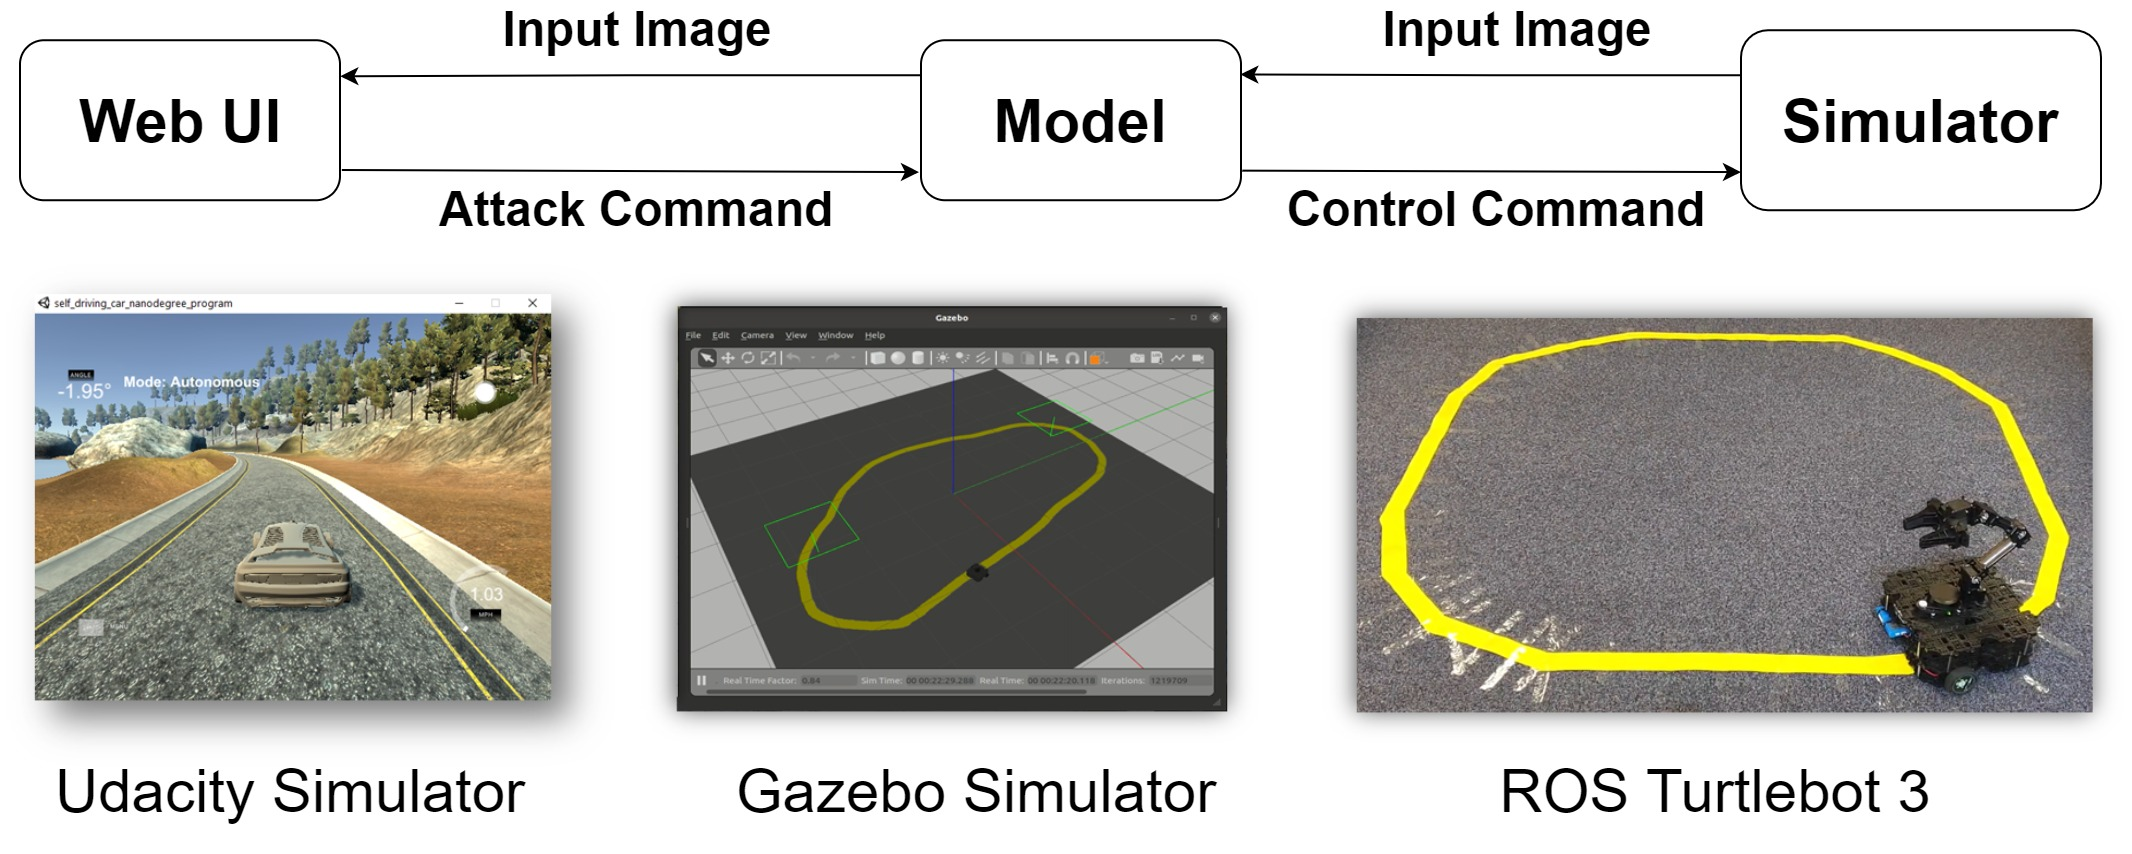
\includegraphics[width=\textwidth]{figures/chapter_driving/architechture.jpg}
    \caption{The architecture of the Adversarial Driving System. We tested our attacks in three environments: the Udacity Simulator, the ROS Gazebo Simulator, and a real Turtlebot 3.}
    \label{fig:arch}
\end{figure}

We design an adversarial system to attack the end-to-end autonomous driving system (See Fig. \ref{fig:arch}). The system consists of three key components: the simulator, the server, and the Web User Interface (UI). The simulator publishes the image captured by the front camera to the server. Meanwhile, it accepts steering commands from the server to manipulate the vehicle. The modular design pattern makes it possible to conveniently replace the simulator with a real Turtlebot without breaking the whole system. The server receives input images from the simulator via WebSocket connections and then sends back the control commands. Meanwhile, it receives attack commands from the web browser and then injects the adversarial perturbation into the input image. The end-to-end driving model is deployed on the server as well. We use a website as a front-end where the attacker can monitor the status of the simulator and choose different attacks.
% The experimental results are presented in the next section.

\section{Experimental Results}

This section first describes the training of the driving systems. Following this, we evaluate the performance of our proposed image-specific and image-agnostic attacks.

% \begin{figure*}[b]
%     \centering
%     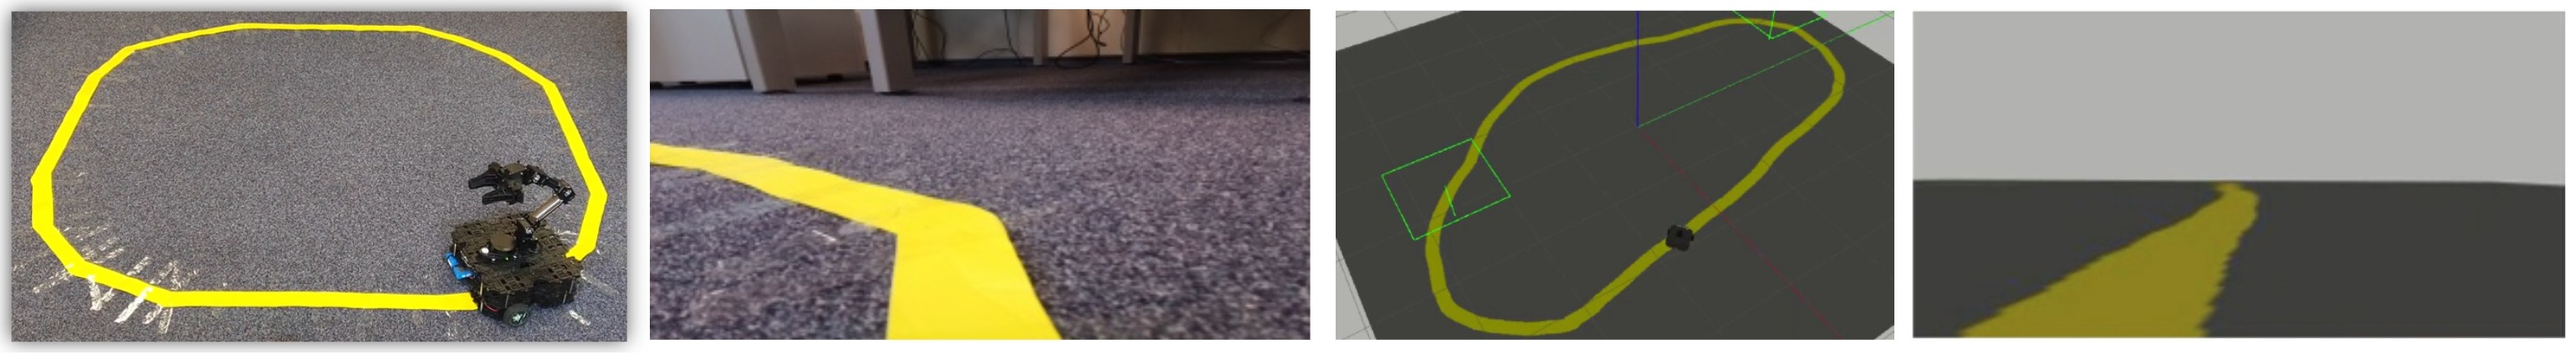
\includegraphics[width=\textwidth]{figures/chapter_driving/ros_turtlebot.jpg}
%     \caption{Our test platforms and input images in ROS: A real turtlebot and ROS Gazebo Simulator.}
%     \label{fig:turtlebot}
% \end{figure*}

%\vspace{-1ex}

\subsection{Model Training}

Our objective is to implement a real-time online attack against an end-to-end imitation learning model. Since it is risky to perform online attacks against real-world driving systems, we tested our attacks in self-driving simulators. 

The target imitation learning models were trained from human driving records. In total, we collected 32k images of human driving records in our test environments: the Udacity Simulator (8k), the Gazebo Simulator (12k), and a real Turtlebot 3 (12k). We then trained one end-to-end driving model for each individual environment. The structure of the driving model is detailed in Table \ref{table_NVIDIA_model}.
Our experiments showed that all three models were vulnerable to adversarial attacks. 

In the following sections, we use the data from the Udacity Simulator to analyze the attack since experiments in this environment are easier to reproduce and examine than using a Turtlebot for other researchers. The experiments conducted using the Gazebo simulator are illustrated in the demo video.

% Fig. \ref{fig:turtlebot} illustrates the input image we collected in Gazebo Simulator and from a real Turtlebot 


\begin{table}[H]
\begin{center}
\begin{tabular}{ c c c }
     \hline
     Layer & Output Shape & Parameters \\ 
     \hline
     Input & (None, 160, 320, 3) & 0 \\  
     Conv2D & (None, 78, 158, 24) & 1824 \\  
     Conv2D & (None, 37, 77, 36) & 21636 \\  
     Conv2D & (None, 17, 37, 48) & 43248 \\  
     Conv2D & (None, 15, 35, 64) & 27712 \\  
     Conv2D & (None, 13, 13, 24) & 36928 \\
     Dropout & (None, 13, 13, 24) & 0 \\
     Flatten & (None, 27456) & 0 \\
     Dense & (None, 100) & 2745700 \\
     Dense & (None, 50) & 5050 \\
     Dense & (None, 10) & 510 \\
     Dense & (None, 1) & 11 \\
     \hline
    \end{tabular}
    \caption{The structure of the end-to-end driving model. \label{table_NVIDIA_model}}
\end{center}
\end{table}

\clearpage

\subsection{The Image-Specific Attack}

To begin with, we demonstrate that applying random noise to the end-to-end driving model only results in very small deviations. The parameter $\epsilon$ is used to ensure that the total disturbance of the random noise is the same as from the image-specific attack. Specifically, note that the image-specific attack adds or subtracts $\epsilon$ from each pixel based on the sign of the gradient. Likewise, we construct a random noise perturbation that randomly adds or subtracts $\epsilon$ from each pixel. 

\begin{figure}[tbph]
    \centering
    \begin{subfigure}[b]{\textwidth}
        \centering
        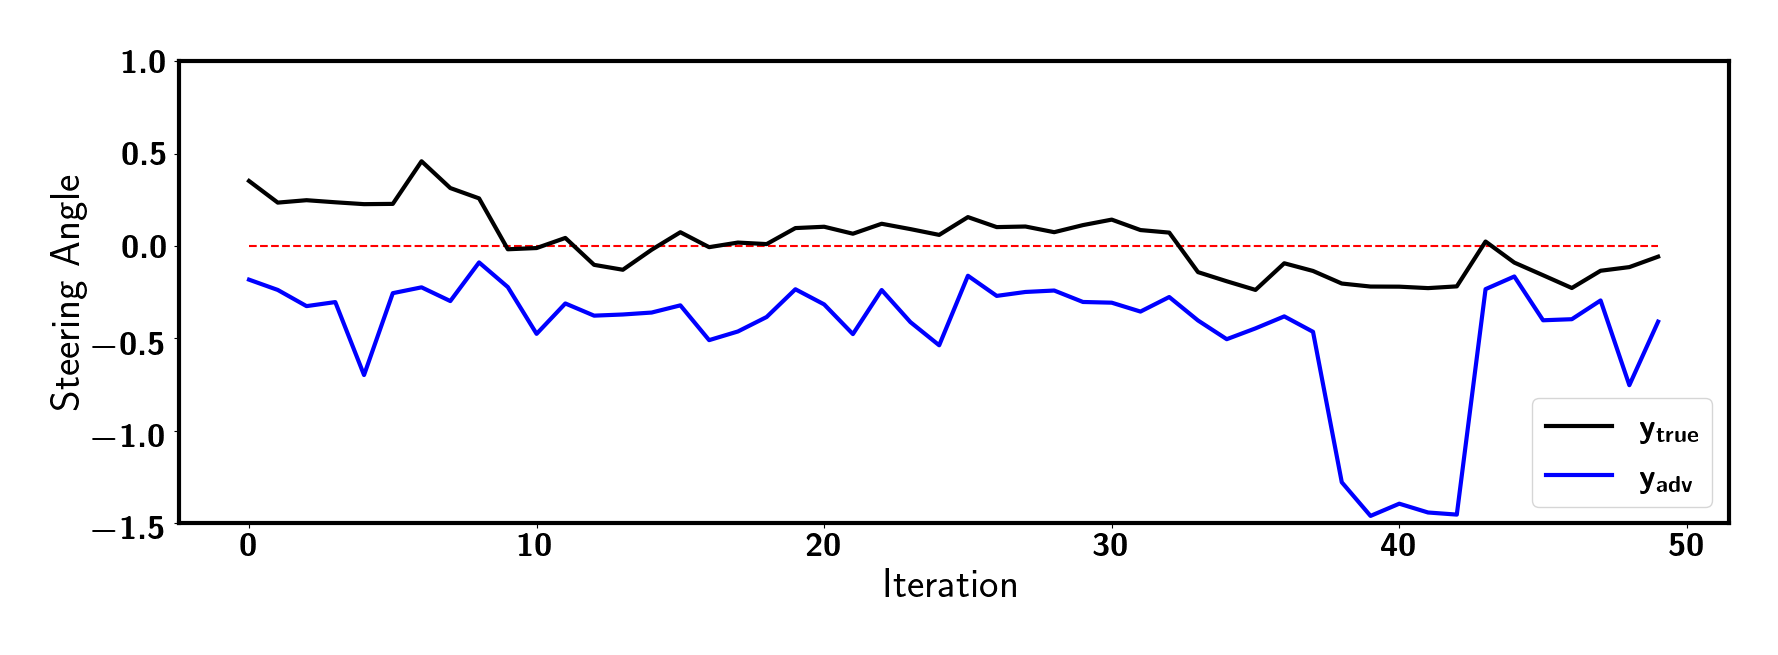
\includegraphics[width=\textwidth]{figures/chapter_driving/left.png}
        \caption{The image-specific left attack decreases the steering angle.\label{fig:image-specific-left-attack}}
    \end{subfigure}
    \begin{subfigure}[b]{\textwidth}
        \centering
        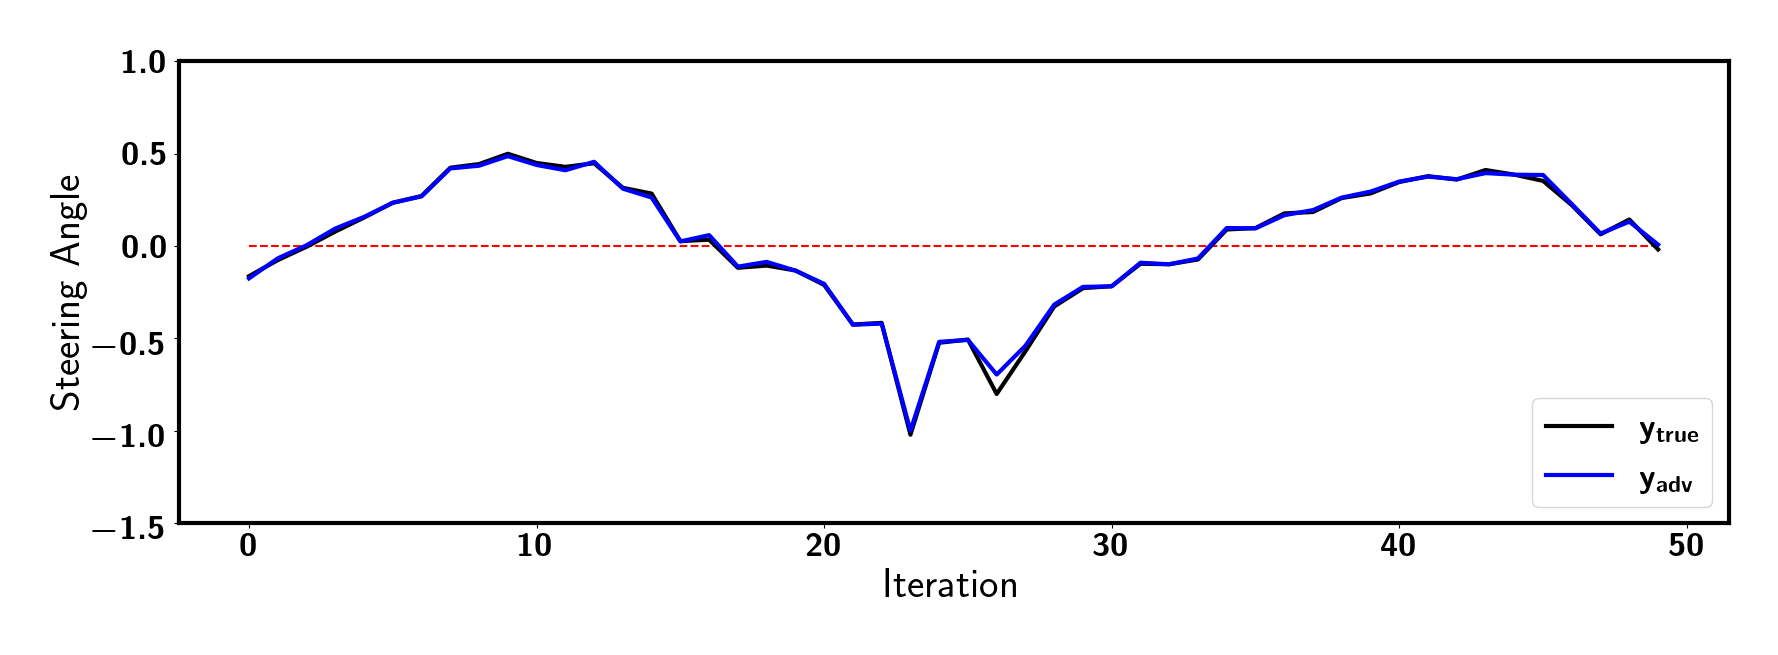
\includegraphics[width=\textwidth]{figures/chapter_driving/random.png}
        \caption{The random noise perturbation barely deviates $y_{adv}$ from $y_{true}$.}
    \end{subfigure}
    \begin{subfigure}[b]{\textwidth}
        \centering
        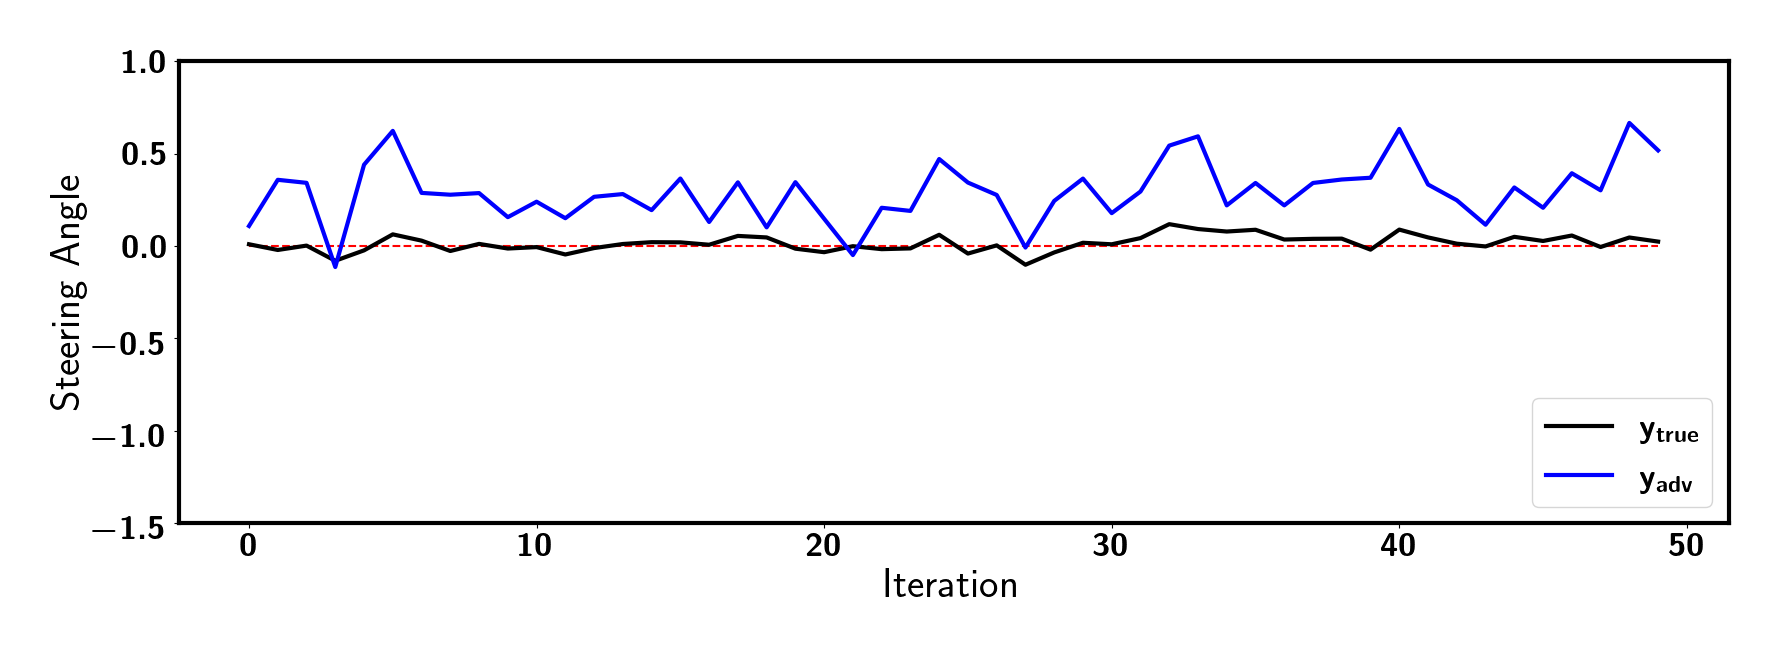
\includegraphics[width=\textwidth]{figures/chapter_driving/right.png}
        \caption{The image-specific right attack increases the steering angle.\label{fig:image-specific-right-attack}}
    \end{subfigure}
    \caption{The image-specific attack and random noise with the same strength ($\epsilon = 1$).}
    \label{fig:image-specific-online}
\end{figure}

In Fig. \ref{fig:image-specific-online}, we applied three different attacks that are of the same strength. Once under the image-specific attack, the vehicle drove off the road in several seconds. The image-specific left attack deviates the vehicle to the left by decreasing the steering angle, thus the $y_{adv}$ is smaller than $y_{true}$ in Fig. \ref{fig:image-specific-left-attack}. On the other hand, the image-specific right attack deviates the vehicle to the right by increasing the steering angle, thus the $y_{adv}$ is greater than $y_{true}$ in Fig. \ref{fig:image-specific-right-attack}. The random noise perturbation barely deviates $y_{adv}$ from $y_{true}$, indicating that it has little effect on the driving model.

The image-specific attack achieved 20-30 FPS on an Intel i7-8665U CPU and 600-700 FPS on an NVIDIA RTX 2080Ti GPU. Since the CPU and GPU are also utilized for Udacity Simulator, the attack performance varies depending on the hardware temperature.

Further, we measured the \acrshort{mad} of the steering angle over 800 attacks. The results are shown in Table \ref{tab:image-specific}. As can be seen, even the weakest image-specific attack ($\epsilon=0.1$) is much stronger than the strongest random noise attack ($\epsilon=8$). When $\epsilon = 4$ and $\epsilon = 8$, we can even deviate the steering angle outside of the range $[-1, 1]$. In other words, the image-specific attack is very strong. However, its weakness is that it needs to calculate the gradients of each individual input image. In a real-world scenario, we may not have access to the input image and gradients. Thus, we propose the image-agnostic attack that trains the perturbation using driving records and does not need access to the input and gradients during the deployment.

\begin{table}[H]
    \centering
    \begin{tabular}{ccc}
    \hline
    Attack Strength & Random Noise Attack & Image-Specific Attack\\
    \hline
    \ $\epsilon=0.1$    & 0.0002    & 0.1448 \\
    \ $\epsilon=1$      & 0.0020    & 0.4779 \\
    \ $\epsilon=2$      & 0.0048    & 0.7329 \\
    \ $\epsilon=4$      & 0.0150    & 1.4895 \\
    \ $\epsilon=8$      & 0.0278    & 2.4469 \\
    \hline
    \end{tabular}
    \caption{The \acrfull{mad} of the steering angle over 800 image-specific attacks.}
    \label{tab:image-specific}
\end{table}

% \pagebreak

\clearpage

\null
\vfill

\begin{figure}[H]
    \centering

    \begin{subfigure}[b]{\textwidth}
        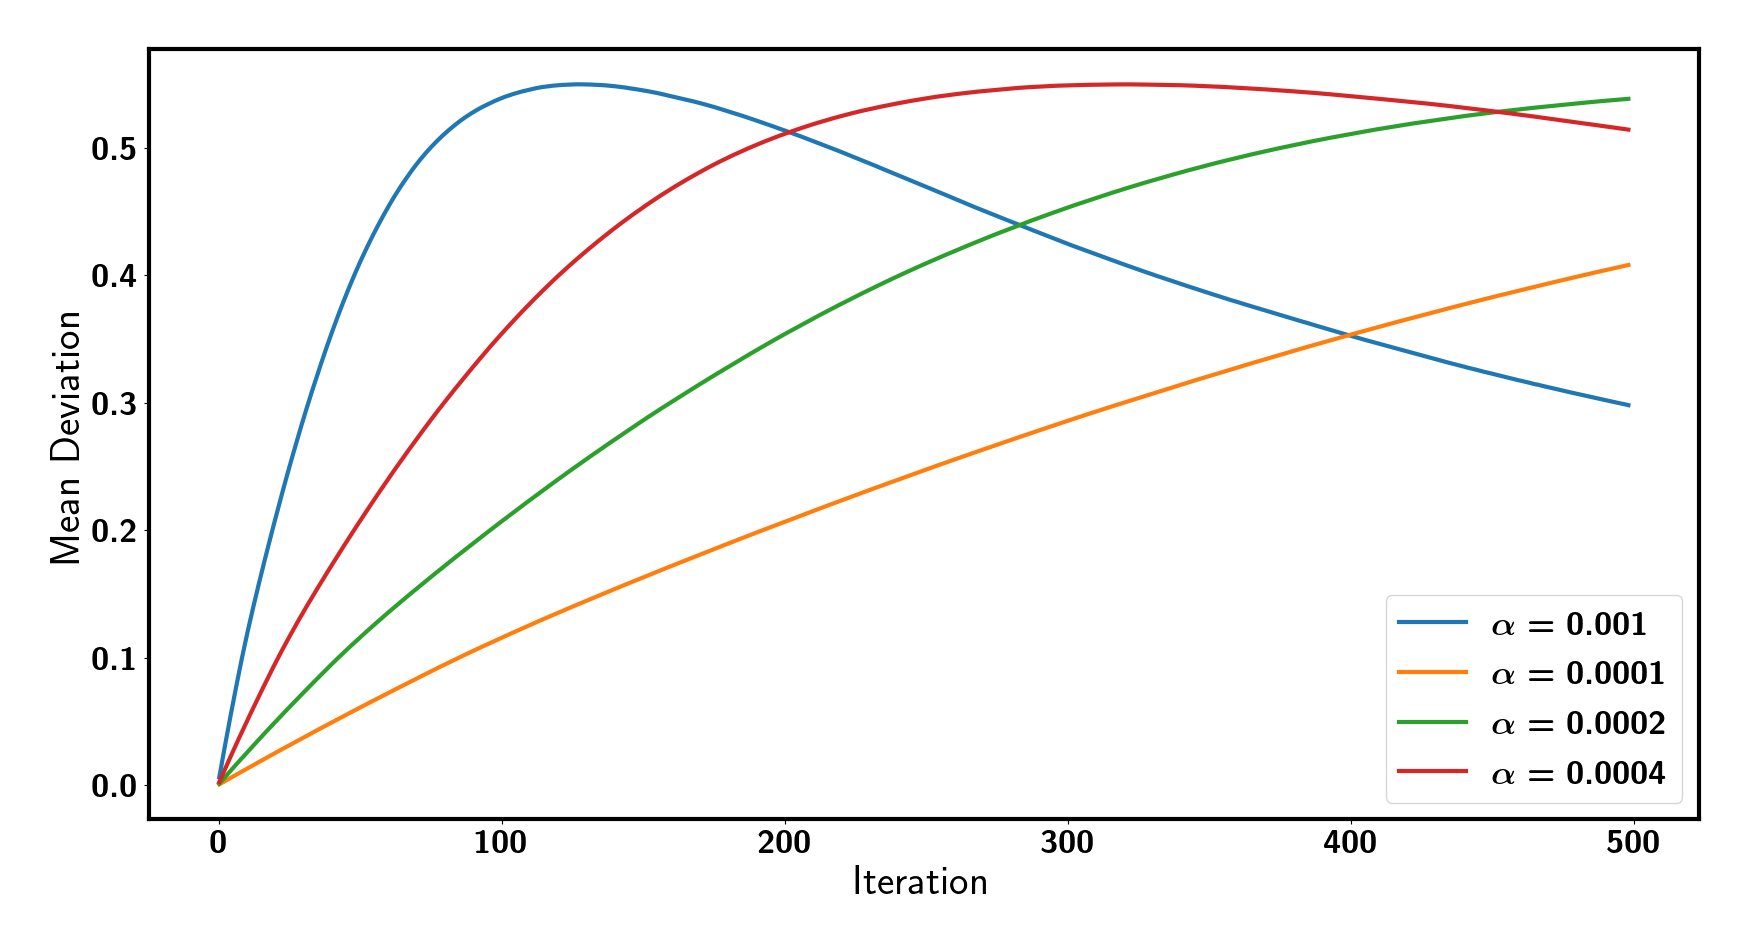
\includegraphics[width=\textwidth]{figures/chapter_driving/alpha.png}
        \caption{Different $\alpha$ with fixed $\epsilon=1, \xi=4$.}
        \label{fig:random}
    \end{subfigure}

    \begin{subfigure}[b]{\textwidth}
        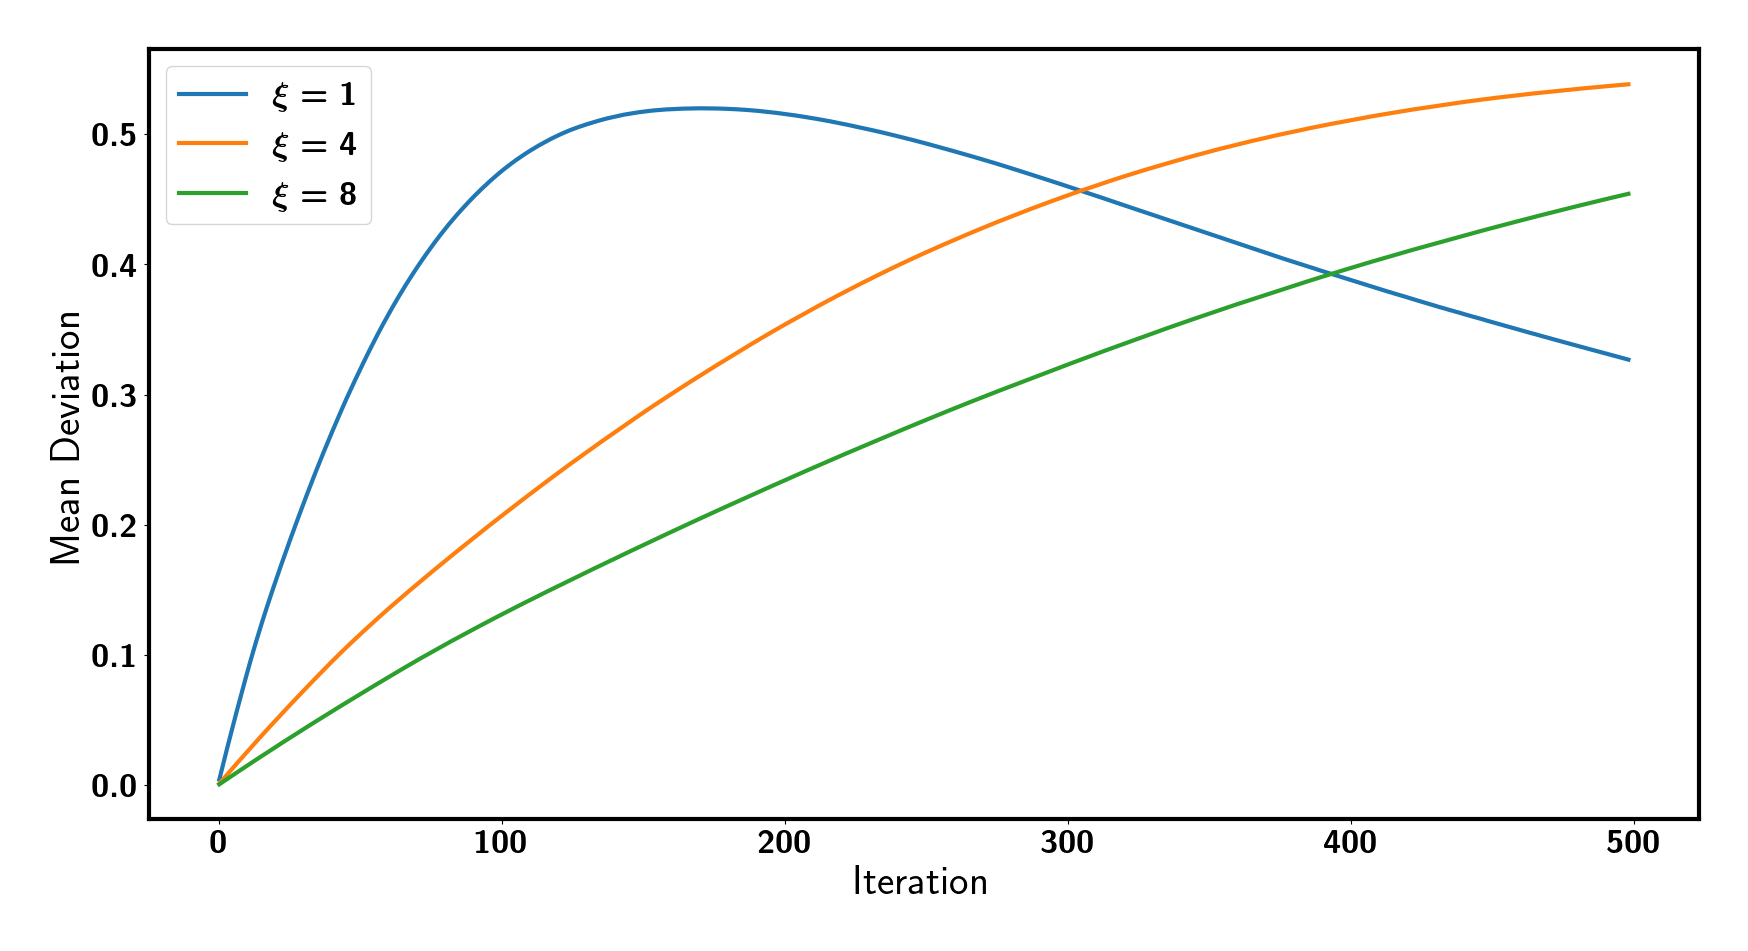
\includegraphics[width=\textwidth]{figures/chapter_driving/xi.png}
        \caption{Different $\xi$ with fixed $\alpha=0.002$}
        \label{fig:left}
    \end{subfigure}

    \caption{The mean deviation of the steering angle during the training process with different hyperparameters.\label{figure_hyperparameters}}
\end{figure}

\vfill

\clearpage

\null
\vfill

\begin{figure}[H]
    \centering
    \begin{subfigure}[b]{\textwidth}
        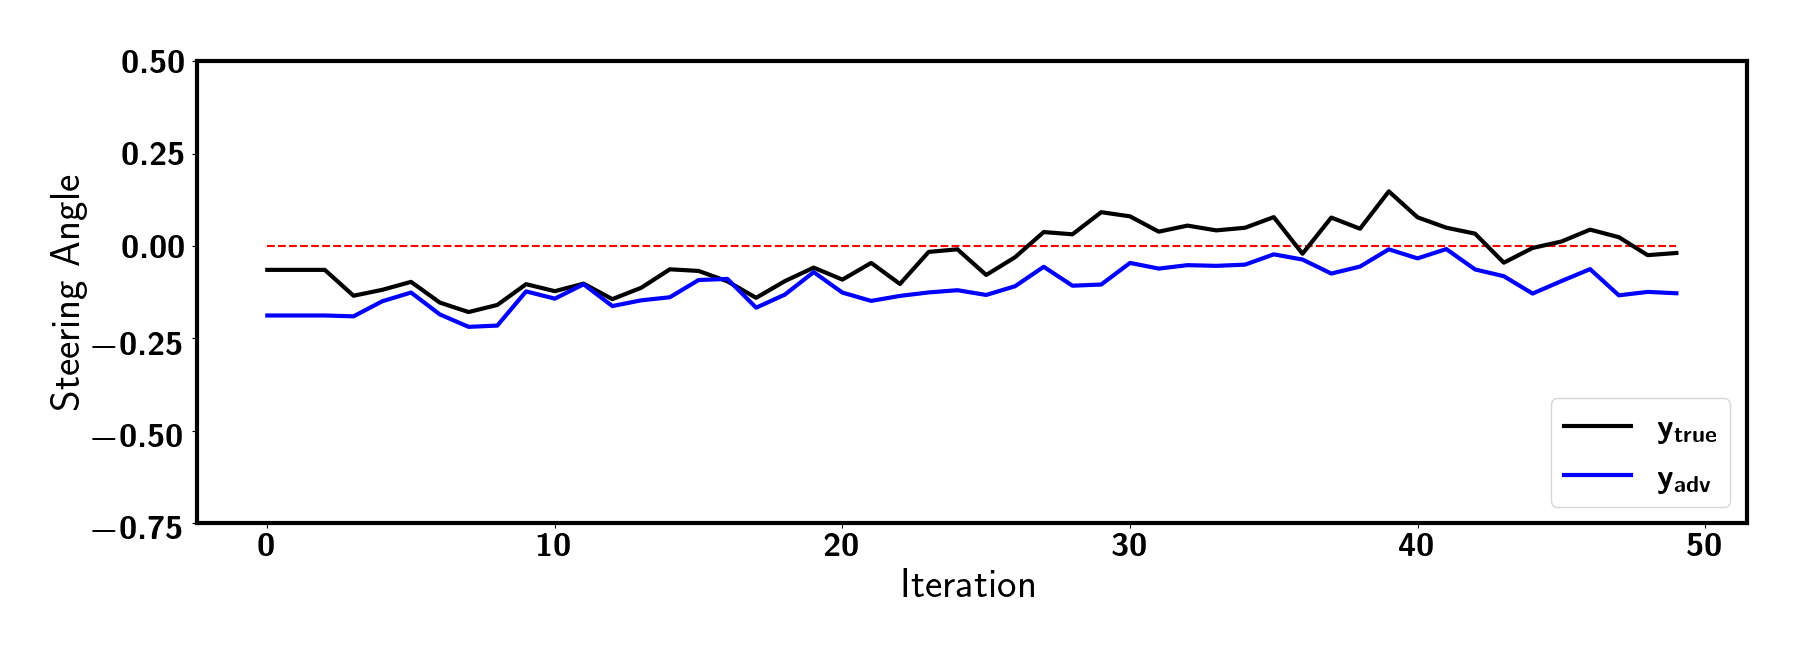
\includegraphics[width=\textwidth]{figures/chapter_driving/uni_left.png}
        \caption{The image-agnostic Left Attack decreases the model output ($y_{adv}<0$), making it difficult to turn right. ($\epsilon=1)$}
        \label{fig:uni_left}
    \end{subfigure}
    \begin{subfigure}[b]{\textwidth}
        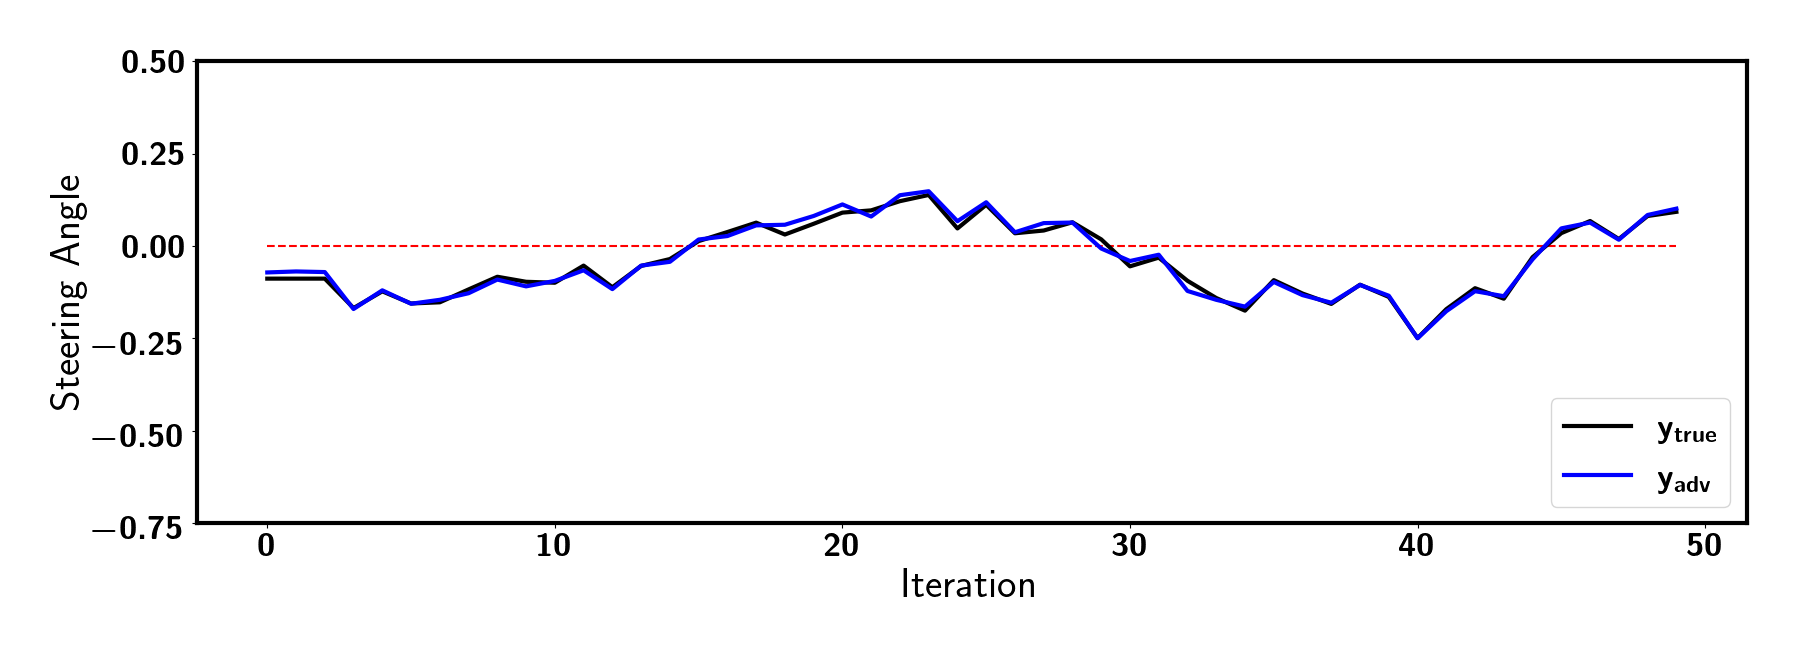
\includegraphics[width=\textwidth]{figures/chapter_driving/uni_random.png}
        \caption{The random noises barely deviates $y_{adv}$ from $y_{true}$.}
        \label{fig:uni_random}
    \end{subfigure}
    \begin{subfigure}[b]{\textwidth}
        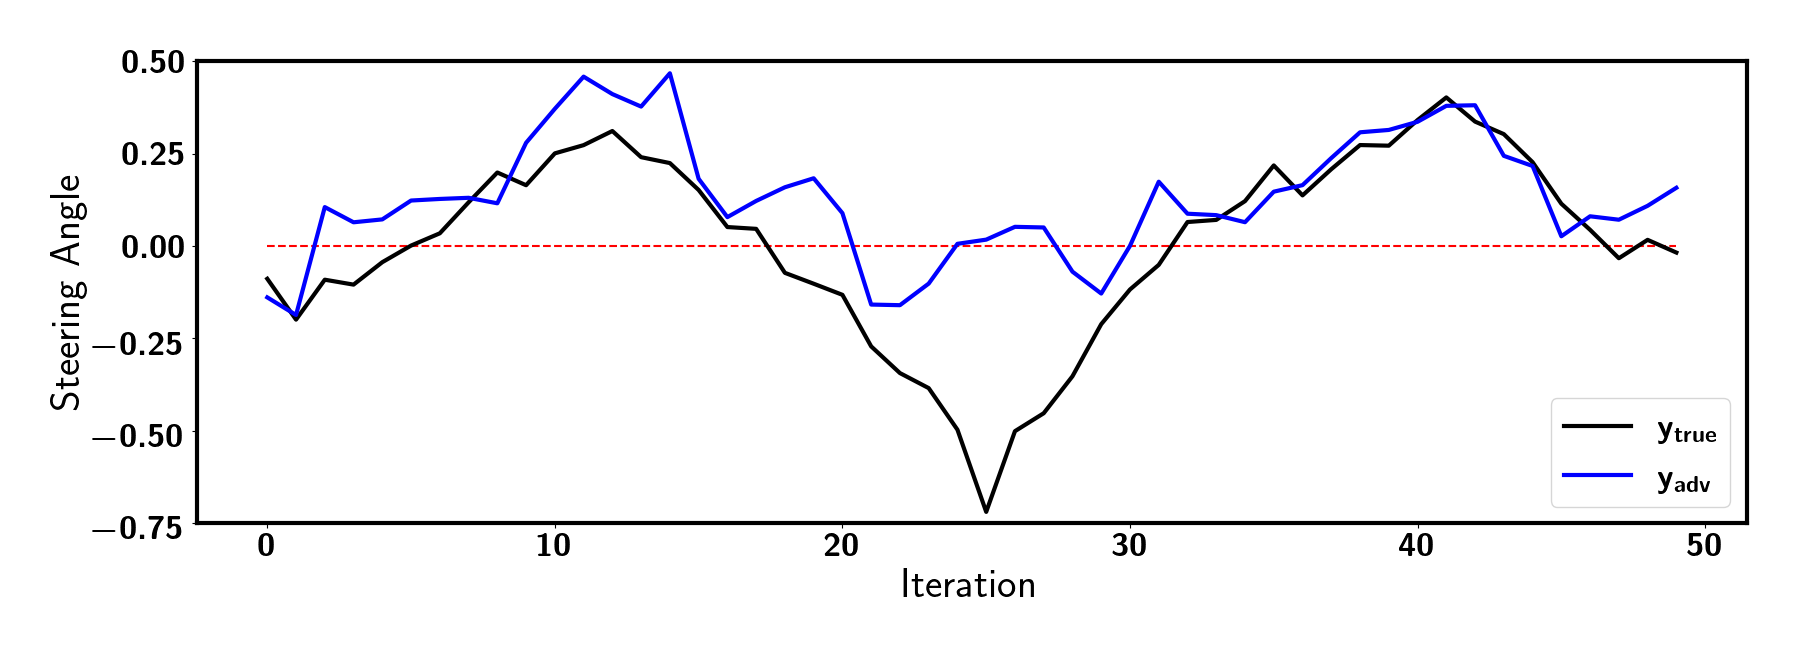
\includegraphics[width=\textwidth]{figures/chapter_driving/uni_right.png}
        \caption{The image-agnostic Right Attack increases the model output ($y_{adv}>0$), making it difficult to turn left. ($\epsilon=1)$}
        \label{fig:uni_right}
    \end{subfigure}
    \caption{The Image-Agnostic attack ($\alpha=0.002$, $\xi=4$, $n=500$) and random noises with the same strength ($\epsilon = 1$).}
    \label{fig:image-agnostic-online}
\end{figure}

\vfill

\subsection{The Image-Agnostic Attack}

In similarity with the image-specific attack, the strength of the image-agnostic attack was also compared with a random noise attack.
The results are shown in Table \ref{tab:image-agnostic}. Though the image-agnostic attack is weaker than the image-specific attack, it is still stronger than the random noise attack.

\begin{table}[H]
    \centering
    \begin{tabular}{ccc}
    \hline
    Attack Strength & Random Noise Attack & Image-Agnostic Attack\\
    \hline
    \ $\epsilon=0.1$    & 0.0002    & 0.0373 \\
    \ $\epsilon=1$      & 0.0020    & 0.1109 \\
    \ $\epsilon=2$      & 0.0048    & 0.1294 \\
    \ $\epsilon=4$      & 0.0150    & 0.1131 \\
    \ $\epsilon=8$      & 0.0278    & 0.1275 \\
    \hline
    \end{tabular}
    \caption{The \acrfull{mad} of the steering angle over 800 image-agnostic attacks ($\alpha=0.002,\ \xi=4$, $n=500$).}
    \label{tab:image-agnostic}
\end{table}

% We then tested different learning rate decay.

% Vheicles reaction to the attack

% As a result, the end-to-end driving model is vulnerable to adversarial attacks.

% \clearpage

As seen in Table \ref{tab:image-agnostic}, the strength of the image-agnostic attack does not improve after $\epsilon > 2$. This is due to the limited generalizability of the perturbation. Increasing the strength of the attack further may increase the model output for some inputs but may equally well decrease the model for other inputs. Therefore, increasing $\epsilon$ further adds more variation to the model prediction while the \acrshort{mad} remains stable.

We also investigated the effect of the learning rate $\alpha$ and the step size $\xi$ on the training process (See Fig. \ref{figure_hyperparameters}). The learning rate $\alpha$ controls the variation of the perturbation during the whole iteration. We tested different $\alpha$ with fixed parameters $\epsilon=1$ and $\xi=4$. As $\alpha$ increases, the mean deviation increases faster. However, the iteration process also becomes more variable, and the mean deviation decreases after 100 steps when $\alpha>0.01$. 

The step size $\xi$ decides how fast the perturbation is updated to change the model output to the desired direction for each input image $x$. A smaller $\xi$ makes the update towards the target direction more steady, but the iteration takes a longer time. A larger $\xi$ can change the direction of the model output in a single step, but the perturbation may not generalize well to other inputs.

As illustrated in Fig. \ref{fig:image-agnostic-online}, using the parameters $\alpha=0.0002$ and $\xi=4$ enabled us to generate image-agnostic perturbations at $\epsilon=1$ that are comparable in performance with the image-agnostic attack at $\epsilon=0.1$. While the image-agnostic is not as strong as the image-specific attack, the image-agnostic attack makes the vehicle difficult to control at sharp corners (this is illustrated in the demo video), which could lead to incidents at some critical points. 

In addition, the image-agnostic attack applies the same perturbation to all frames. Thus, the deployment of the image-agnostic attack is much more computationally efficient than the image-specific attack.

% \pagebreak

% \addtolength{\textheight}{-2cm}

% \clearpage

\section{Conclusions}

This paper has demonstrated that it is possible to attack an end-to-end driving model in real-time. We devise a strong image-specific attack and a stealthy image-agnostic attack. Though the mean absolute deviation of the image-agnostic attack is smaller than the image-specific attack, both attacks are more effective than random noise attacks. The image-agnostic attack deviates the vehicle outside of the lane after just a few seconds, while the image-agnostic attack could cause incidents at sharp corners. These results provide new evidence of the vulnerability of safety-critical robotic applications.


% \clearpage

% \printbibliography[
%   keyword={chapter_driving}, heading=subbibintoc, resetnumbers=true
% ]

%% MAIN CONTENT CHAPTERS
\chapter{Adversarial Detection}
\label{chpt:detection}

% \newrefsection

In this chapter, we focus on adversarial attacks against object detection systems. The task of object detection consists of object localization and object classification. The object detection model locates the position of each object and classifies which category the object belongs to. Besides attacking the classification task, we also need to deviate localization results. Thus, it's more challenging than adversarial attacks against image classification models.

Another challenge is where and how we apply the adversarial perturbation. Unlike image classification task that receives static images as input, object detection systems usually process a real-time video stream from the camera. Though we have various approaches to generate the perturbation, it won't pose a threat against real-world applications if we cannot apply the perturbation in real-time.

Starting with an introduction to existing object detection models and related white-box adversarial attacks, we then try to achieve an online attack that generates the perturbation in real-time. Besides, we explore the possibility of producing a single \acrfull{uap} that could attack all the frames received from a camera and inject the perturbation via a Human-in-the-Middle hardware attack.

% Lastly, we introduce the WHite-box Adversarial Toolbox (WHAT) that integrates our attacks into an open-source toolbox.

% \section{Introduction}

% Deep neural networks have been widely adopted in the task of object detection, and achieving SOTA performance. However, it's no more a secret that deep learning models are vulnerable to adversarial attacks. It has been nearly 8 years since the first adversarial attack against neural networks \citep{goodfellow2015explaining}. We can fool a deep learning model by adding small perturbations to the original input image. The perturbation is unperceivable by human eyes but can lead the detection model to inaccurate results.

% Based on where we apply the attack, current adversarial attacks can be classified into two categories: digital perturbation and physical perturbation. For digital perturbation, we apply perturbation in the digital world. The perturbation does not exist in the actual world. It is applied to the digital image captured by the camera. For physical perturbation, we apply the perturbation in the physical world. For instance, we print out the adversarial perturbation on a poster \citep{lee2019physical} or T-shirt \citep{xu2020adversarial}.

% \begin{figure}[H]
% \centering
% 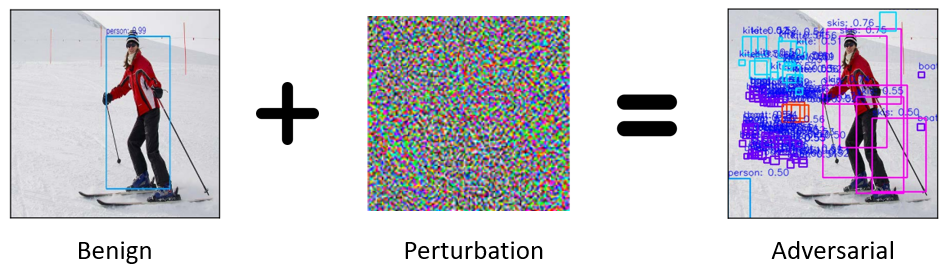
\includegraphics[scale=0.8]{figures/chapter_detection/digital.png}
% \caption{Digital Perturbation: The perturbation is added directly to the input image of the model.}
% \label{fig.adv_digital}
% \end{figure}

% \begin{figure}[H]
% \centering
% 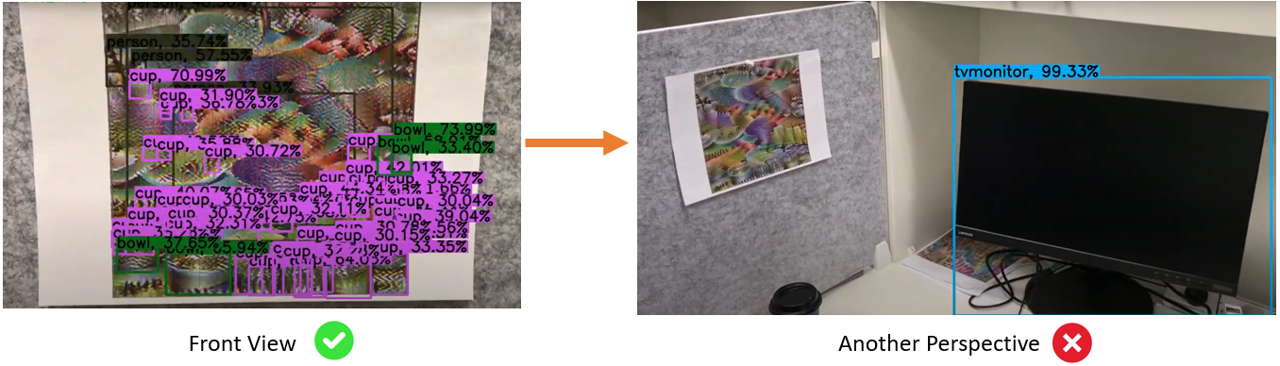
\includegraphics[scale=0.45]{figures/chapter_detection/physical.png}
% \caption{Physical Perturbation: The perturbation is printed on objects in real world.}
% \label{fig.adv_physical}
% \end{figure}

% However, there are several disadvantages to both attacks. Digital perturbation is applied directly to the input image of the detection model \citep{lu2017no}. The problem is that the input of the model is inside the operating system, which we do not have access to. It's not trivial to hack into the system of Google's Self-Driving Car and apply the perturbation. As a result, the biggest hurdle for digital perturbation is that we cannot add the perturbation into a real system. This renders digital perturbation useless in practice. Research interests are shifting from digital perturbation to physical perturbation. 

% No need to worry about adversarial attacks

% Inherent disadvantages exist for physical attacks as well. For physical attacks, the perturbation is inflexible and it's perceivable by the human eyes. Once the adversarial poster is printed out, we cannot change it unless we reprint it. This could take a long time during the trial-and-error process. Due to the inflexibility of physical perturbation, it may only work if the adversarial poster is placed within a limited range and from a specific perspective. As illustrated in Figure \ref{fig.adv_physical}, if the camera captures the image from another perspective, the adversarial poster becomes a normal poster. Besides, physical perturbations are perceivable by humans. Both adversarial posters and adversarial T-shirts look quite unusual compared with normal ones. Wearing an adversarial T-shirt on the street immediately draws others' attention. 

% In summary, digital perturbation is flexible and inconspicuous, but impractical. Physical perturbation is more practical but inflexible and conspicuous. In this research, we would like to investigate if it is possible to bring digital perturbations to the real world so that we achieve a flexible and inconspicuous attack in the real world.

% \subsection{Object Detection Models}

% Before introducing adversarial attacks, it's worthwhile to get familiar with target object detection models. Existing frameworks of object detection can be categorized into two types: region proposal-based methods and regression/classification-based methods \citep{Zhao2019}. We can either solve localization and classification problems separately or simultaneously. If we first generate a series of region proposals and then classify each proposal into different categories, this is a region proposal-based method (Two-stage). On the other hand, if we regard object detection as a classification or regression task that outputs locations and categories simultaneously, this is a regression/classification-based method (One-stage). The PASCAL VOC dataset and MS COCO dataset are used for a benchmark among different models.

% \begin{figure}[H]
% \centering
% 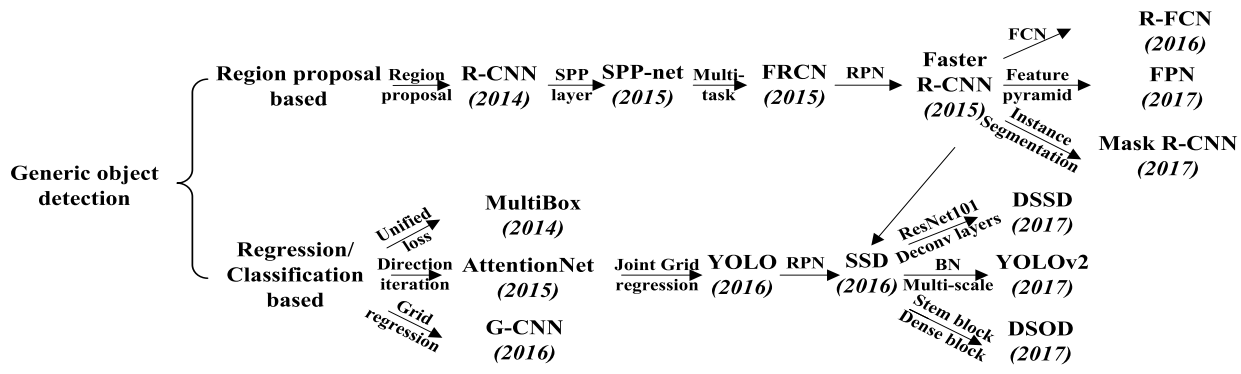
\includegraphics[scale=0.6]{figures/chapter_detection/detection_review.png}
% \caption{Two types of frameworks: region-proposal based (two-stage) and regression / classification based (one-stage) \citep{Zhao2019}.}
% \label{fig.detection_frame}
% \end{figure}

% OverFeat \citep{overfeat2014} is one of the first papers that use Convolution Neural Network on object detection. They use a multi-scale and sliding window approach to scan over the image and find locations of objects in regression layers. This is computationally expensive as most sub-sections of the input image do not contain any object. A more efficient approach is to first generate region proposals, regions that could contain objects, and then extract features from these proposals for regression. Selective search \citep{uijlings2013selective} is a common approach to generate region proposals, and it's employed in R-CNN \citep{girshick2014rich} as well. 

% \begin{figure}[H]
% \centering
% 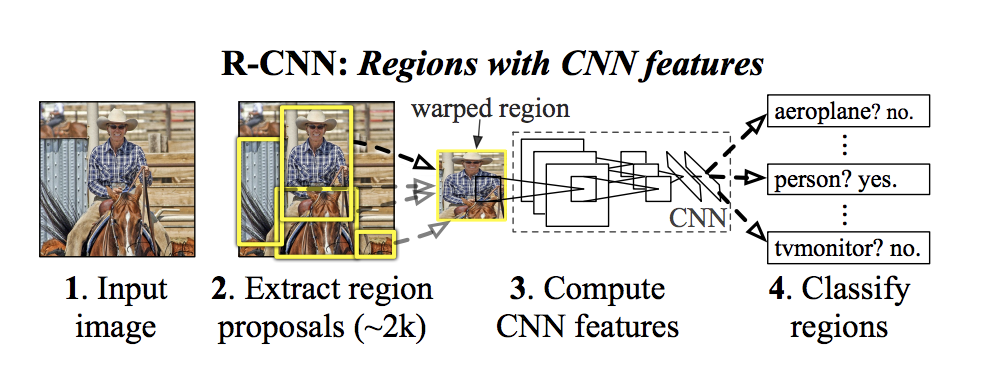
\includegraphics[scale=0.45]{figures/chapter_detection/rcnn.png}
% \caption{The architecture of RCNN \citep{girshick2014rich}.}
% \label{fig.rcnn}
% \end{figure}

% RCNN generates around 2000 region proposals using selective search. It's more efficient than the sliding window method, but still computationally expensive. The same author of RCNN then proposed Fast-RCNN \citep{girshick2015fast} to improve the efficiency. RCNN feeds 2000 region proposals into CNN to compute features, while Fast-RCNN only feeds the original input image once to the CNN to generate feature maps, making it more efficient. To further improve its efficiency, region proposal computation becomes the bottleneck. Thus, Faster-RCNN \citep{ren2015faster} employs Region Proposal Network (RPN) that takes an image of arbitrary size to generate a set of rectangular object proposals.

% \begin{figure}[H]
% \centering
% 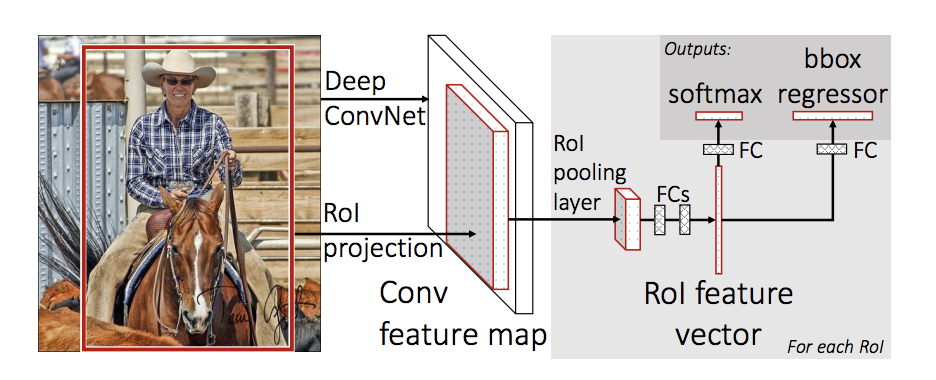
\includegraphics[scale=0.4]{figures/chapter_detection/fast-rcnn.png}
% \caption{The architecture of Fast-RCNN \citep{girshick2015fast}.}
% \label{fig.fastrcnn}
% \end{figure}

% FPN is not an object detector by itself. It is a feature extractor that works with object detectors. FPN extracts feature maps and later feeds into a detector, says RPN, for object detection. 

% In contrast, regression/classification-based methods generate detection results in a single run, making it even more efficient. Region proposal-based frameworks consist of region proposal generation, feature extraction with CNN, classification, and bounding box regression. Different components are usually trained separately. This becomes the bottleneck for real-time applications.  Experimental results demonstrate that two-stage models are more accurate, while one-stage models are more efficient. Here, we introduce the two most widely deployed one-stage models: YOLO \citep{redmon2016you} and SSD \citep{liu2016ssd}. 

% YOLO divides the input image into SxS grids. Each grid cell is supposed to predict objects at the center of each grid cell. To handle different aspect ratios of objects, YOLO predefines several anchor boxes at 3 different scales. Each grid cell outputs the confidence value, bounding boxes, and probability vectors of different classes. For example, if an input image of size 416x416 is divided into grid cells of shape 13x13, we have 32x32 grid cells in total. Suppose we have 9 predefined anchors, 3 at each scale, the YOLO model produces 32x32x9 = 9216 outputs, each output includes the confidence value, the position and shape of the bounding box, and the probability vector for each class. If we have 80 classes, each output is a vector of size 80 + 4 +1 = 85. All the outputs are then handled by NMS boxes to eliminate duplicated boxes and boxes that have a low confidence value of containing objects.

% \begin{figure}[H]
% \centering
% 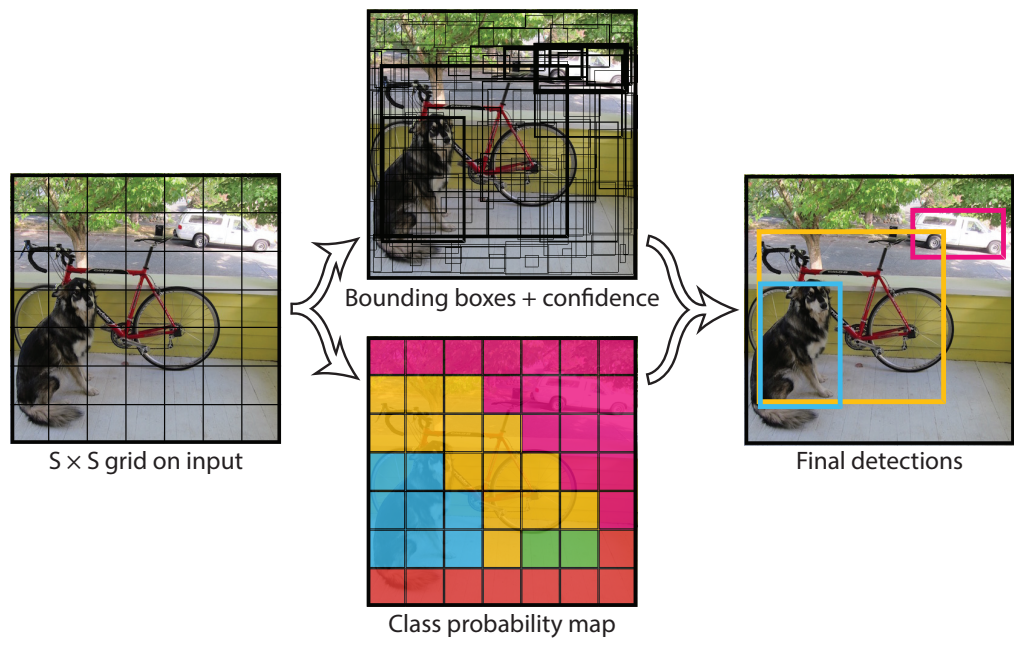
\includegraphics[scale=0.6]{figures/chapter_detection/yolo.png}
% \caption{The architecture of YOLO \citep{redmon2016you}.}
% \label{fig.yolo}
% \end{figure}

% SSD is another one-stage detection model that can outperform Faster-RCNN on both PASCAL VOC and MS COCO dataset with hard negative mining, data augmentation, and carefully chosen anchors, but much more efficient.

% \begin{figure}[H]
% \centering
% 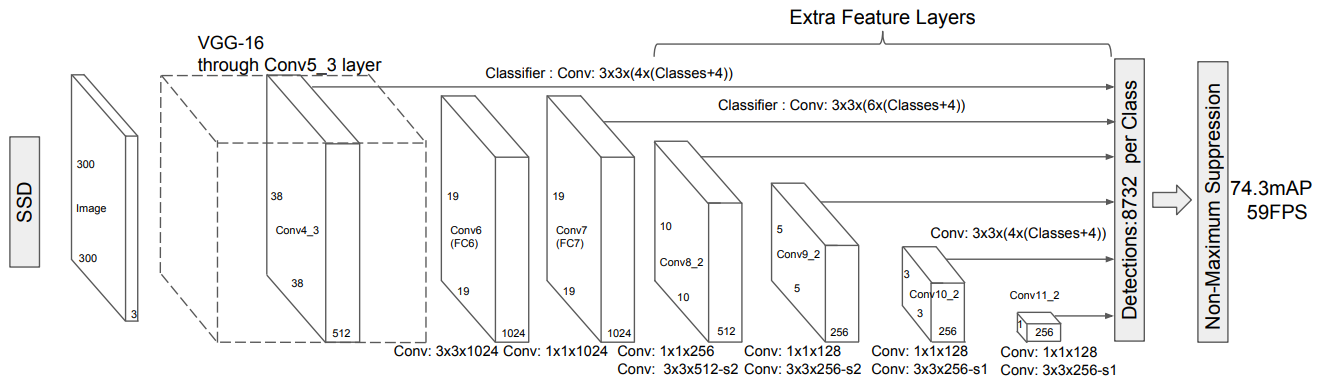
\includegraphics[scale=0.6]{figures/chapter_detection/ssd.png}
% \caption{The architecture of SSD \citep{liu2016ssd}.}
% \label{fig.ssd}
% \end{figure}

% However, both one-stage and two-stage models are vulnerable to adversarial attacks. In this research, we test adversarial attacks against both types of models. In other words, we choose Faster-RCNN, Mask-RCNN \citep{he2017mask}, YOLO and SSD as our target models.


% \subsection{White-box Adversarial Attacks}

% Adversarial attacks against object detection are still in their inchoate stage. The first adversarial attack against neural networks was published in 2014 that targets image classification models. A lot of following works on adversarial attacks have emerged since then. Most of them still attack image classification models. We find the first adversarial attack against image segmentation in 2017 \citep{fischer2017adversarial}, and an evaluation of the transferability of adversarial attacks against segmentation and detection \citep{gurbaxani2018traits} in 2018. More adversarial attacks against object detection arises since 2019, and most of them target two-stage detection models. More specifically, the Region Proposal Network (RPN) in Faster RCNN.

% The Dense Adversary Generation (DAG) \citep{xie2017adversarial} method intends to misclassify objects by adding small perturbations to the input image. It deviates predictions of $n$ target objects from ground-truth class label $l_n$ by reducing the error between $l_n$ and $l^{'}_{n}$, where $l^{'}_{n}$ denotes adversarial labels that can be randomly sampled from other incorrect labels. The DAG attack against segmentation models is relatively easy because the attack can be achieved by assigning each pixel to a different class. While for object detection models that output several thousands of bounding boxes, fooling one bounding box is not enough as the rest could still make correct predictions. This problem is solved by attacking the Region Proposal Network (RPN) in FasterRCNN, where they increase the threshold of NMS in RPN, such that they attack several thousands of bounding boxes simultaneously.

% The Robust Adversarial Perturbation (RAP) \citep{li2018robust} attacks the RPN as well. It fools the RPN to predict most objects as background and produces wrong estimations on bounding boxes even if correct foreground objects are proposed. This is achieved by optimizing the following loss function:

% \begin{equation} 
% min_\mathcal{I} \quad L_{label}(\mathcal{I};\mathcal{F}_{\theta}) + L_{shape}(\mathcal{I};\mathcal{F}_{\theta}), \quad s.t. \ \ PSNR(\mathcal{I}) \geq \epsilon
% \end{equation}

% \begin{equation}
%     L_{label}(\mathcal{I};\mathcal{F}_{\theta}) = \sum_{j=1}^{m} z_j log(s_j)
% \end{equation}

% \begin{equation}
%     L_{shape}(\mathcal{I};\mathcal{F}_{\theta}) = \sum_{j=1}^{m} z_j((\Delta x_j - \tau_x)^2 + (\Delta y_j - \tau_y)^2 + (\Delta w_j - \tau_w)^2 + (\Delta h_j - \tau_h)^2)
% \end{equation}

% The Unified and Efficient Adversary (UEA) \citep{ijcai2019-134} methods extends DAG with a feature loss to train a generative adversarial network (GAN) to generate adversarial examples. 

% The above methods generate one adversarial perturbation for each image, thus the perturbation is image-specific. It is also possible to generate a universal perturbation that is image-agnostic. The adversarial objectness gradient attack (TOG)\citep{chow2020adversarial} iterates over the training set to generate a single perturbation that can fool all the images in the training set. The Universal Dense Object Suppression (U-DOS) \citep{LI2021107584} uses a similar approach, but it focuses on fooling objects to be the background. It is also possible to only attack specific objects using TAR \citep{mohamad2021}.

% Here's a summary of the aforementioned adversarial attacks against object detection models:

% - TAR \citep{mohamad2021} - 2021

% - U-DOS \citep{LI2021107584} - 2021

% - TOG \citep{chow2020adversarial} - 2020

% - UEA \citep{ijcai2019-134} - 2019

% - RAP \citep{li2018robust} - 2018

% - DAG \citep{xie2017adversarial} - 2017

% Though these methods generate digital perturbations, similar approaches can be utilized to produce physical perturbations. If we print out digital perturbations on a poster, it won't be a valid physical perturbation. Valid physical perturbations can be generated by adding extra constraints to the loss function, such as the Sub-sampled Non-Printability Score (SNPS). The Non-Printability Score (NPS) is employed to measure the error between a printed pixel and its digital counterparts. Thus the adversarial effect of digital perturbations can be preserved after being printed out.

% In summary, different adversarial attacks define distinct loss functions that determine the objective of their attack. The loss functions are minimized in similar ways, and if we add constraints on the Non-Printability Score (NPS), we can generate phjmysical perturbations.

% \clearpage

\section{Real-time White-box Attacks in ROS}
\label{sec:adv_detect}

Intelligent robots rely on object detection models to perceive the environment. Following advances in deep learning security it has been revealed that object detection models are vulnerable to adversarial attacks. However, prior research primarily focuses on attacking static images or offline videos. Therefore, it is still unclear if such attacks could jeopardize real-world robotic applications in dynamic environments. This project bridges this gap by presenting the first real-time online attack against object detection models. We devise three attacks that fabricate bounding boxes for nonexistent objects at desired locations. The attacks achieve a success rate of about 90\% within about 20 iterations. 

% The demo video is available at \href{https://youtu.be/zJZ1aNlXsMU}{https://youtu.be/zJZ1aNlXsMU}.

% Our objective is to fool the YOLOv3 \citep{redmon2018yolov3}, and YOLOv4 \citep{bochkovskiy2020yolov4} object detection models to mistakenly detect objects at locations where there is no object. We generate adversarial overlays by combining the imperceptibility of adversarial filters with the localizability of adversarial patches.

\begin{figure}[H]
    \centering
    \begin{subfigure}[b]{\textwidth}
        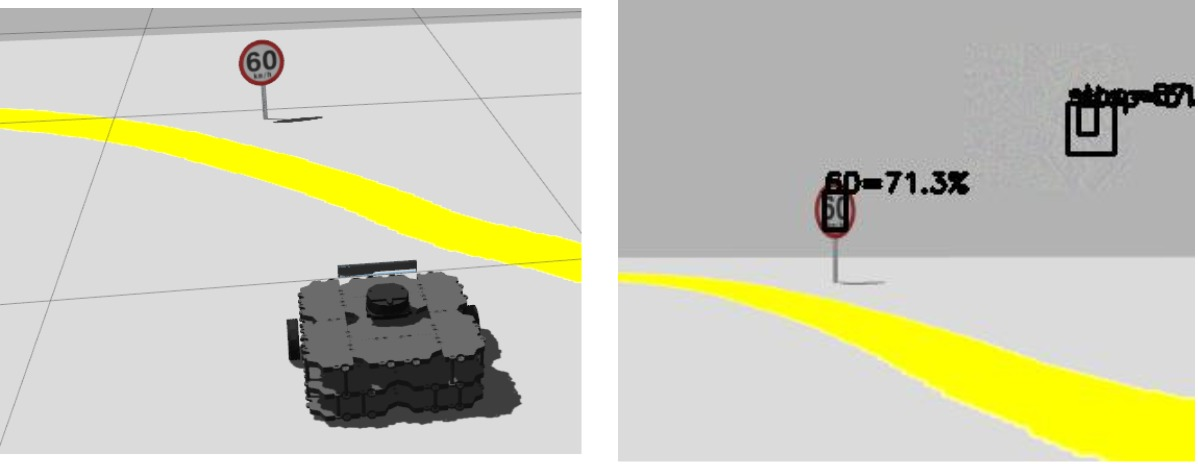
\includegraphics[width=\textwidth]{figures/chapter_detection/detection/one.jpg}
        \caption{The \textbf{original image} (left) only contains one traffic sign. The \textbf{One-Targeted} Attack (right) generates one overlay containing several target objects (stop sign).}
        \label{fig:sparse-untar} 
    \end{subfigure}

    \begin{subfigure}[b]{\textwidth}
        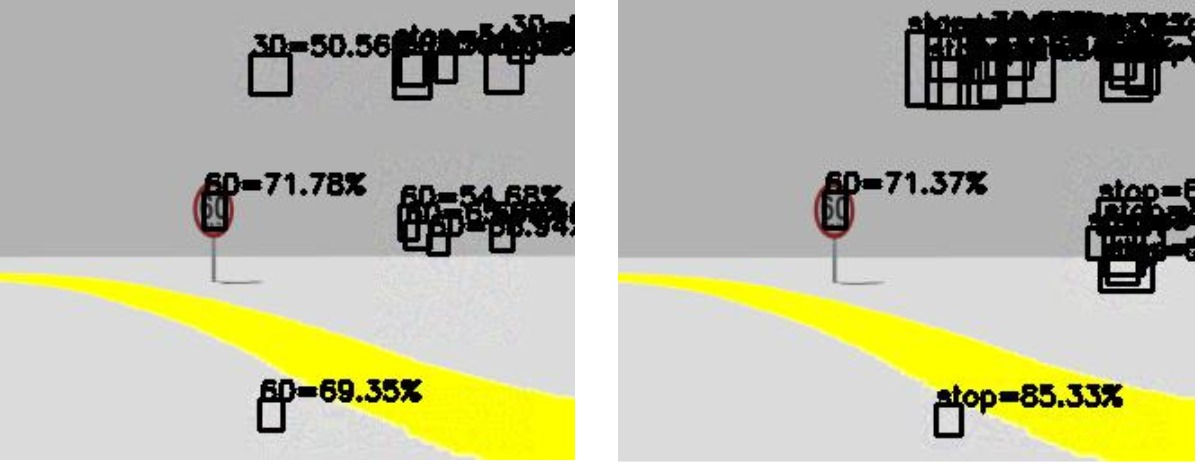
\includegraphics[width=\textwidth]{figures/chapter_detection/detection/multi.jpg}
        \caption{The \textbf{Multi-Untargeted} Attack (left) generates multiple overlays containing different kinds of objects (30, 60, stop). The \textbf{Multi-Targeted} Attack (right) generates multiple overlays containing several target objects (stop sign).}
        \label{fig:dense-untar}
    \end{subfigure}
    \caption{This paper demonstrates how to generate adversarial overlays of arbitrary shapes at specified positions in real time.}
    \label{fig:detection.overview}
\end{figure}

\subsection{Introduction}

Reliable object detection is crucial for multiple safety-critical robotic applications. For example, an autonomous driving system relies on object detection models to perceive the environment and take action on it. While advances in deep neural networks have rapidly increased the availability of high-accuracy object detection models, this breakthrough has also revealed several potential vulnerabilities. The first adversarial attacks fooled image classification models by adding imperceptible perturbations to the input image \citep{GoodfellowSS14}. Later research removed the restriction to imperceptible perturbations and instead designed an adversarial patch that can be printed in the physical world \citep{brown2017patch}. The physical patch fooled an image classification model to misclassify the most salient object in the image. However, attacks against image classification models cannot fool object detection models. Therefore, in 2018, Liu et al. introduced the DPatch, a digital patch that fools object detection models \citep{liu2018dpatch}, and Lee et al. later extended the attack to physical patches \citep{lee2019physical}.

The generation of adversarial patches for attacking real-time robotic applications is still a rather challenging task. The generation process itself is often very computationally expensive. In addition, the efficiency of the physical patch is conditioned on strict requirements on the relative distance and orientation of the camera and the patch \citep{wang2021daedalus} \citep{threet2021physical}. These requirements are often difficult to satisfy for real-world robotic applications deployed in dynamic environments.

Recent research in penetration tests against the Robot Operating System (ROS) has shown that it is possible to inject digital patches into the ROS message that contains the camera image \citep{dieber2020penetration}. In particular, Dieber et al. succeeded in isolating a ROS node so that they could intercept and manipulate the ROS message that contains sensor data while the victim node is unaware of the attack. In this paper, we generate digital overlays (unperceivable digital patches) at desired locations in real time and then exploit the vulnerability to inject the digital overlays into the input image. Overall, this paper makes the following contributions:
\begin{itemize}
    \item We devise three adversarial attacks that can generate digital overlays of different shapes at specified locations in real time (see Fig. \ref{fig:detection.overview}). This extends previous research that primarily has focused on square patches.
    \item We investigate the adversarial effect of digital overlays of different sizes and aspect ratios. In particular, it is found that the size of the overlay is critical for the success of the attack, whereas the attack performance is independent of the aspect ratio. 
    \item We test our attacks in the Robot Operating System (ROS). The system is open-sourced to facilitate future extensions and comparisons\footnote{Our source code on GitHub: \url{https://github.com/wuhanstudio/adversarial-detection}}.
\end{itemize}

\subsection{Preliminaries}
\label{section_preliminaries}

This section clarifies the differences between adversarial filters and adversarial patches. Following this, we describe how prior research applies these filters and patches in the digital and physical world. Our research focuses on applying adversarial patches in the digital world.

\subsubsection{The Adversarial Filter}

An adversarial filter refers to a perturbation added to the entire image. Thus, the adversarial filter is of the same size as the input image and is unperceivable by human eyes. Based on where we apply the perturbation, adversarial filters can be categorized as digital or physical filters.

\textbf{Digital Filter} (Fig. \ref{fig:digital_filter}): The first adversarial attack against image classification models was a digital filter that added a small perturbation to the entire input image \citep{GoodfellowSS14}. The perturbation can be generated using either gradient-based methods \citep{madryMSTV18} \citep{kurakin2018adversarial} \citep{wong2019wasserstein} \citep{croce2020reliable} or optimization-based methods \citep{papernot2016transferability} \citep{carlini2017towards} \citep{qin2019imperceptible}. Prior research uses the $l_1$, $l_2$, and $l_{\infty}$ norms to measure the human perceptual distance between the adversarial and the original input image \citep{miyato2015distributional} \citep{sabour2015adversarial} \citep{chen2018ead}. While the digital filter first proved the existence of adversarial examples, it is limited in practical scenarios since it is not always possible to assume access to the input image.

\textbf{Physical Filter} (Fig. \ref{fig:physical_filter}): Physical filters attach a translucent film to the camera lens to perturb the entire image \citep{li2019adversarial}. While physical filters do not require access to the input image, they do require physical access to the camera. One big challenge with physical filters is the difficulty of manufacturing a film that precisely replicates the adversarial perturbation. Thus, the practical applicability of adversarial filters in the physical world is still rather limited. In addition, to the best of our knowledge, physical filters has so far only been used to attack image classification models, not object detection models. 

% \pagebreak

\subsubsection{The Adversarial Patch}

In some scenarios, it is possible to remove the constraint of the imperceptibility of the perturbation. This means that we can generate so-called patches that are clearly distinguishable to anyone viewing the image in question. 

Contrary to filters, these patches are limited in size and only perturb part of the image, allowing us to better control the location of generated objects when attacking an object detection model. Similar to filters, patches can be categorized as digital or physical patches.

\textbf{Digital Patch} (Fig. \ref{fig:digital_patch}) In 2018, Liu etc al. designed the DPatch \citep{liu2018dpatch} to attack the Faster R-CNN object detection model \citep{ren2015faster}. The DPatch is location-independent, which means that it can be placed anywhere in the input image. Another notable digital patch is the TOG attack, presented in 2020 by Chow et al \citep{chow2020adversarial}. They generated a 40x40 adversarial patch to fool object detection models into misclassifying objects to which the patch was attached.

\textbf{Physical Patch} (Fig. \ref{fig:physical_patch}) In 2017, Google presented landmark research for generating a physical patch to attack an image classification model \citep{brown2017patch}. As a result, research interest gradually shifted to from digital to physical patches. Later, Lee et al. \citep{lee2019physical} and Wang et al. \citep{wang2021daedalus} extended the physical patch attack from image classification to object detection. One shortcoming of physical patches is their inflexibility. Once the adversarial patch has been printed out, the only way to change it is through reprinting. To improve their flexibility, Hoory et al. dynamically displayed adversarial patches on a flat screen attached to a car \citep{hoory2020dynamic}.

In conclusion, research on adversarial attacks initially focused on the design of digital perturbations. Later, adversarial perturbations were extended from digital attacks to the physical world. In the next section, we describe a process for generating unperceivable digital patches at desired locations in real-time.

% \clearpage

\begin{figure}[H]
    \centering
    \begin{subfigure}[b]{\textwidth}
        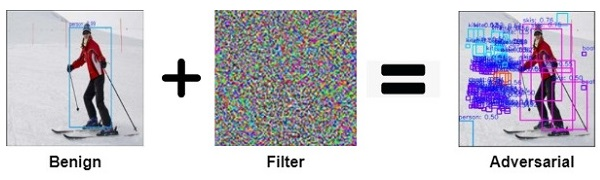
\includegraphics[width=\textwidth]{figures/chapter_detection/detection/digital_filter.jpg}
        \caption{Digital filters apply the perturbation to the entire input image in the digital world \citep{wang2021daedalus}.}
        \label{fig:digital_filter}
    \end{subfigure}
    \begin{subfigure}[b]{\textwidth}
        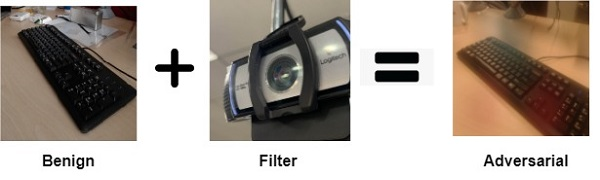
\includegraphics[width=\textwidth]{figures/chapter_detection/detection/physical_filter.jpg}
        \caption{Physical filters apply the perturbation by attacking the camera using, e.g., a translucent film attached to the camera lens \citep{li2019adversarial}.}
        \label{fig:physical_filter}
    \end{subfigure}
    \caption{Adversarial filters perturb the entire image.}
    \label{fig:filter}
\end{figure}

\begin{figure}[H]
    \centering
    \begin{subfigure}[b]{\textwidth}
        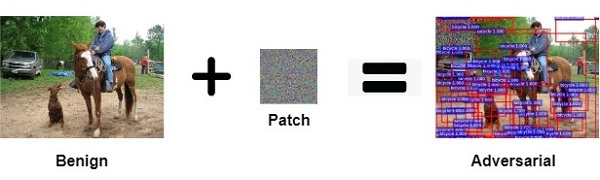
\includegraphics[width=\textwidth]{figures/chapter_detection/detection/digital_patch.jpg}
        \caption{Digital patches replace a part of the input image with the adversarial patch (left top corner) \citep{liu2018dpatch}.}
        \label{fig:digital_patch}
    \end{subfigure}
    \begin{subfigure}[b]{\textwidth}
        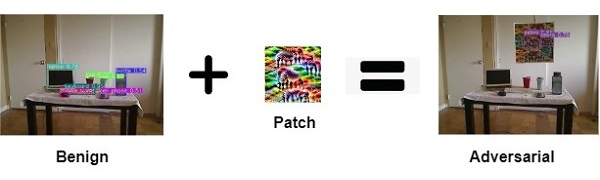
\includegraphics[width=\textwidth]{figures/chapter_detection/detection/physical_patch.jpg}
        \caption{Physical patches print the adversarial patch on a physical object, e.g., on a poster \citep{lee2019physical}.}
        \label{fig:physical_patch}
    \end{subfigure}
    \caption{Adversarial patches perturb part of the image.}
    \label{fig:patch}
\end{figure}

% \clearpage

\subsection{Problem Formulation} 

Our objective is to fool the YOLOv3 \citep{redmon2018yolov3}, and YOLOv4 \citep{bochkovskiy2020yolov4} object detection models to mistakenly detect objects at locations where there is no object. We generate adversarial overlays by combining the imperceptibility of adversarial filters with the localizability of adversarial patches.

The YOLO object detection model splits the input image into $S$x$S$ grids and makes predictions for each grid. For example, the input shape of YOLO is 416x416x3 (height, width, and channel). If $S=13$, we divide each channel into 13x13 grids, and each grid is 32x32 pixels. To detect objects of different sizes, YOLO makes predictions at three different scales (see Fig. \ref{fig.grid}). The first, second, and third output layer contains 13x13, 26x26, and 52x52 grids, respectively. The first output layer detects larger objects, and the third output layer detects smaller objects. In addition, YOLO pre-defines three anchor boxes ($B=3$) at each scale to detect objects of different aspect ratios. Thus, we have 9 pre-defined anchor boxes for 3 scales. Lastly, each output contains the shape and location of the bounding box, the confidence value, and the probability vector for each class (see Fig. \ref{fig.grid}). For example, if the model is pretrained on the MS COCO dataset \citep{mscoco2014} \citep{moore2020fiftyone} that contains 80 classes ($K=80$), each output contains 85 values consisting of four dimensions ($b_x, b_y, b_w, b_h$), one confidence value ($c$), and 80 probabilities $(p_1, p_2, ..., p_{80})$ for each class.

Putting things together: Given an input image $x$, the object detection model outputs $S$x$S$ candidate bounding boxes $o \in \mathcal{O}$ at three different scales ($S \in \{13,26,52\}$, $B=3$, and $|\mathcal{O}| = \sum_{1 \leq i \leq 3} S_i \times S_i \times B$, where $S_i$ represents the grid size of the $i_{th}$ output layer). Further, each candidate box is
\begin{equation}
 o^i = [b_x^i, b_y^i, b_w^i, b_h^i, c^i, p_1^i, p_2^i, ..., p_K^i],\ 1 \leq i \leq |\mathcal{O}|
\end{equation}
for $K$ classes. For example, the shape of the first output layer is $(S_1,\ S_1,\ B,\ K + 5) = (13,\ 13,\ 3,\ 85)$. The image is divided into 13x13 grids, and the model makes predictions for 3 anchor boxes. Each prediction contains 85 values (85 = 4 + 1 + 80). The adversarial attack aims to generate an adversarial perturbation $\delta \in [-1, 1]^{whc}$ such that the adversarial output $\mathcal{O}(x^{'})$ is different from the original output $\mathcal{O}(x)$.

\begin{figure}[H]
    \centering
    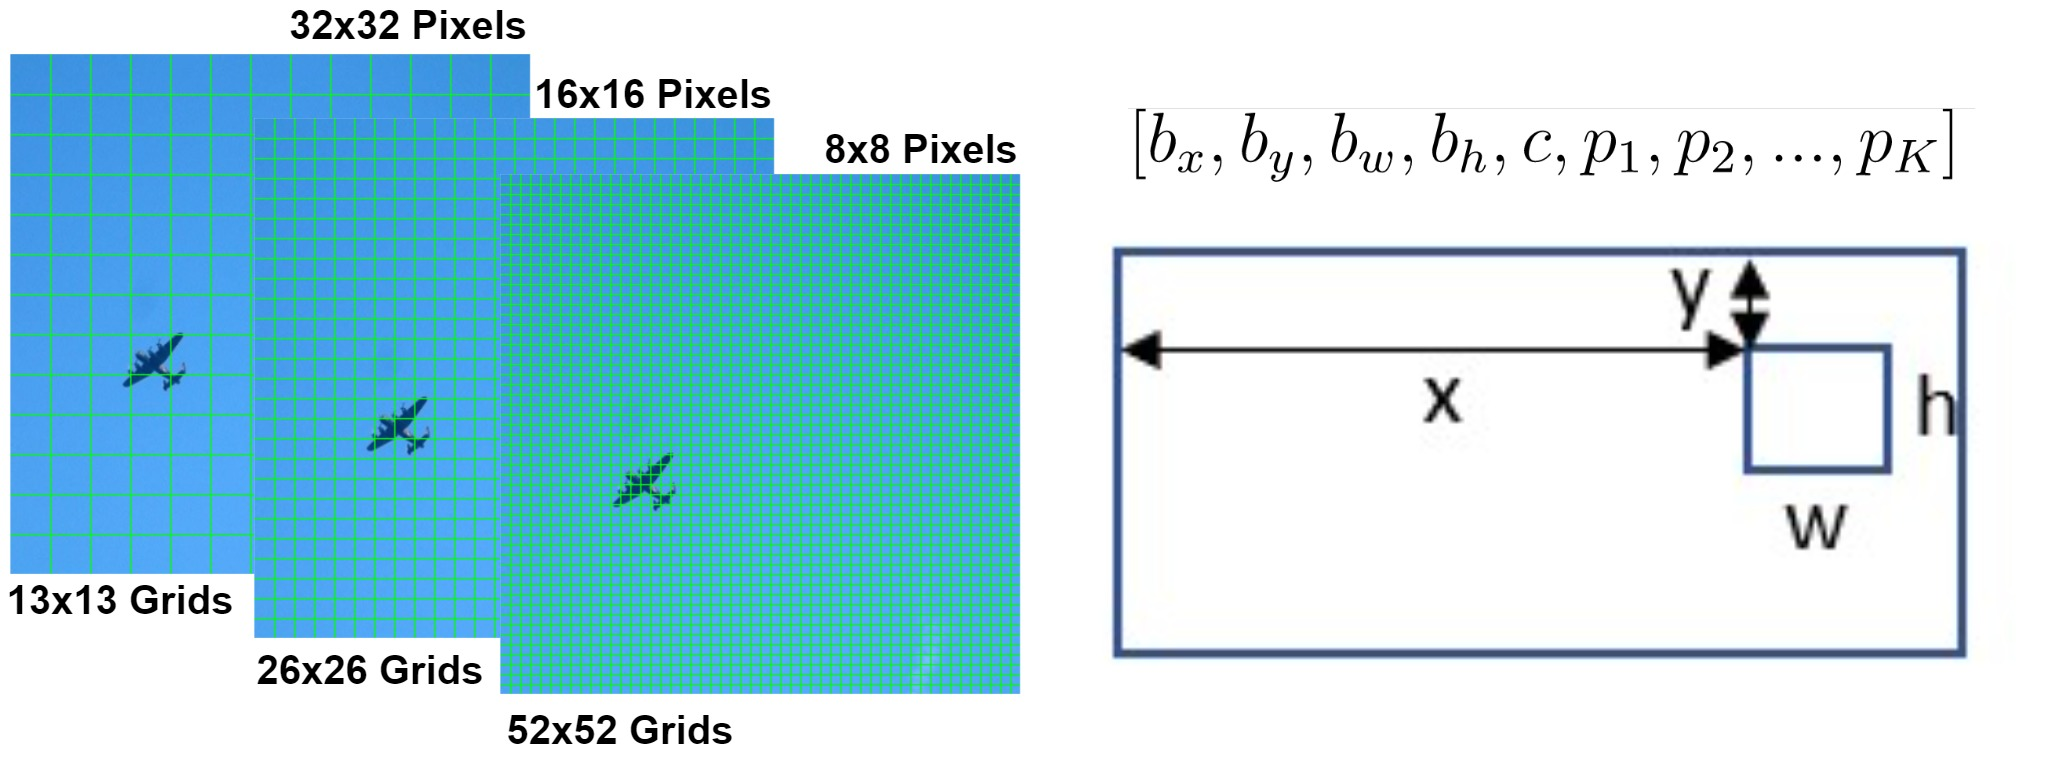
\includegraphics[width=\textwidth]{figures/chapter_detection/detection/grid.jpg}
    \caption{The YOLO object detection model makes predictions at three scales.}
    \label{fig.grid}
\end{figure}

% \pagebreak

\subsubsection{The Adversarial Overlay}

As described in Section \ref{section_preliminaries}, adversarial filters are imperceptible to human eyes but do not allow us to control exactly where in an image that we fabricate objects. Adversarial patches, 
on the other hand, are pinpointable but conspicuous. We propose a new method, the adversarial overlay, that applies an imperceptible perturbation to part of an image. Thereby, the adversarial overlay combines the strengths of adversarial filters and patches and they can be contrasted as: 
\begin{subequations}
\label{eq_perturbations}
\begin{align}
    x^{'}_{filter} &= x + \delta, \\
    x^{'}_{patch} &= (\mathds{1}-m) \odot x + m \odot \delta, \\
    x^{'}_{overlay} &= x + m \odot \delta.
\end{align}
\end{subequations}

Here, the perturbation $\delta$ is applied via a binary mask $m \in \{0, 1\}^{wh}$, and $\odot$ is the Hadamard operator performing element-wise multiplication. 

In equation \eqref{eq_perturbations}, the adversarial filter $x^{'}_{filter}$ applies the perturbation to the entire image without the mask $m$, the adversarial patch $x^{'}_{patch}$ uses the mask to replace part of the image, and the adversarial overlay $x^{'}_{overlay}$ applies the mask to the perturbation and adds it as an overlay to the image.

Now, note that the confidence value and the probability vector collectively determine whether or not a bounding box is drawn on the output image. Thus, by maximizing the product of confidence and probability vector, we can fabricate objects at desired locations. This leads us to three adversarial loss functions $L_{adv}$ for generating perturbations in real time: one loss function for one-targeted attacks
\setcounter{equation}{2}
\begin{equation}
\max_{1 \leq i \leq |\mathcal{O}|}\ [\sigma(c^i) * \sigma(p^i_t)] \label{eq:one-targeted},
\end{equation}
one loss function for multi-targeted attacks 
\begin{equation}
\sum^{|\mathcal{O}|}_{i = 1}\ [\sigma(c^i) * \sigma(p^i_t)] \label{eq:multi-targeted},    
\end{equation}
and one loss function for multi-untargeted attack
\begin{equation}
\sum^{|\mathcal{O}|}_{i = 1} \sum_{j=1}^{K}\ [\sigma(c^i) *\sigma(p^i_j)] \label{eq:multi-untargeted}.    
\end{equation}

% \begin{align*}
% One\ Targeted:\ \mathcal{L}_{adv}^{1}(\mathbfcal{O}) &= \sum^S \max_{1 \leq i \leq |\mathcal{O}|}\ [\sigma(c^i) * \sigma(p^i_t)] \\ 
% Multi\ Targeted:\ \mathcal{L}_{adv}^{2}(\mathbfcal{O}) &= \sum^S \sum^{|\mathcal{O}|}_{i = 1}\ [\sigma(c^i) * \sigma(p^i_t)] \\
% Multi\ Untargeted:\ \mathcal{L}_{adv}^{3}(\mathbfcal{O}) &= \sum^S \sum^{|\mathcal{O}|}_{i = 1} \sum_{j=1}^{K}\ [\sigma(c^i) *\sigma(p^i_j)]
% \end{align*}

%\begin{numcases}{\mathcal{L}_{adv}(\mathbfcal{O})=}
%\sum^B\max_{1 \leq i \leq |\mathcal{O}|}\ [\sigma(c^i) * \sigma(p^i_t)] & \label{eq:one-targeted}\\
%\sum^B \sum^{|\mathcal{O}|}_{i = 1}\ [\sigma(c^i) * \sigma(p^i_t)] & \label{eq:multi-targeted}\\
%\sum^B \sum^{|\mathcal{O}|}_{i = 1} \sum_{j=1}^{K}\ [\sigma(c^i) *\sigma(p^i_j)] \label{eq:multi-untargeted}& 
%\end{numcases}

% where $|\mathcal{O}|$ represents the length of the output that equals to the total number of bounding boxes.

\textbf{The one-targeted attack} (Eq. \ref{eq:one-targeted}) generates the overlay that contains the target object $t \in \{1,\dots,K\}$ by finding the bounding box with the maximum value of $\sigma(c^i) * \sigma(p^i_t)$. It only contains one target object because we increase the confidence and probability of the maximum one in all candidate bounding boxes. 

\textbf{The multi-targeted attack} (Eq. \ref{eq:multi-targeted}) generates multiple overlays that contain target objects $t \in [0, K]$ by maximizing the sum of $\sigma(c^i) * \sigma(p^i_t)$ for the target class.

\textbf{The multi-untargeted attack} (Eq. \ref{eq:multi-untargeted}) generates multiple overlays that contain different objects by maximizing the sum of $\sigma(c^i) * \sigma(p^i_t)$ for all classes.

\clearpage

\begin{algorithm}[H]
    \caption{The Adversarial Overlay Attack}\label{alg:adv-overlay}
    \begin{algorithmic}
        \State Input: The object detection model $f(\theta, x)$, a mask $m$.
        \State Parameters: The number of iterations $n$, the learning rate $\alpha$, and the strength of the attack $\xi$ measured by $l_{\infty}$ norm.
        \State Output: The adversarial perturbation $\delta$.
        \State \textbf{Initialization}: 
        \If {monochrome}
            \State $\delta \leftarrow 0^{416\text{x}416}$
        \Else
            \State $\delta \leftarrow 0^{416\text{x}416\text{x}3}$
        \EndIf
        \For{each input image $x$}
            \State $x' = x$
            \For{each iteration}
                \If {monochrome}
                \State R Channel: $x_R^{'} = x_R' + m \odot \delta$
                \State G Channel: $x_G^{'} = x_G' + m \odot \delta$
                \State B Channel: $x_B^{'} = x_B' + m \odot \delta$
                \Else
                    \State Overlay: $x^{'} = x' + m \odot \delta$
                \EndIf
                \State Gradient: $\nabla = \frac{\partial \mathcal{L}_{adv}(\mathcal{O})}{\partial x'}$
                \If {monochrome}
                    \State $\delta = \delta +  \frac{1}{3}\alpha(\nabla_R + \nabla_G + \nabla_B) $
                \Else
                    \State $\delta = \delta + \alpha \cdot \text{sign}(\nabla)$
                \EndIf
                \State $\delta = \text{clip}(\delta,\ -\xi,\ \xi)$
                \State $x^{'} = \text{clip}(x^{'},\ 0.0,\ 1.0)$
            \EndFor
        \EndFor
    \end{algorithmic}
\end{algorithm}

The function $\sigma (x)$ in the above equations represents the sigmoid function.

Note that it is possible to generate monochrome overlays. Monochrome overlays add the same value to each channel, making the perturbation less conspicuous. We can add the average of the red, green, and blue channels or a single channel since human eyes are most sensitive to the green channel.

The perturbation is computed using gradients. At the end of each iteration, we clip the value of the perturbation so that it does not exceed the pre-defined boundary. The adversarial image of the original DPatch \citep{liu2018dpatch} contains invalid negative pixel values. Thus, we clip the value of the adversarial image to make sure it is still a valid image. The adversarial overlay attack is summarized in Algorithm \ref{alg:adv-overlay}.

% \pagebreak

% \begin{figure}[th]
%     \centering
%     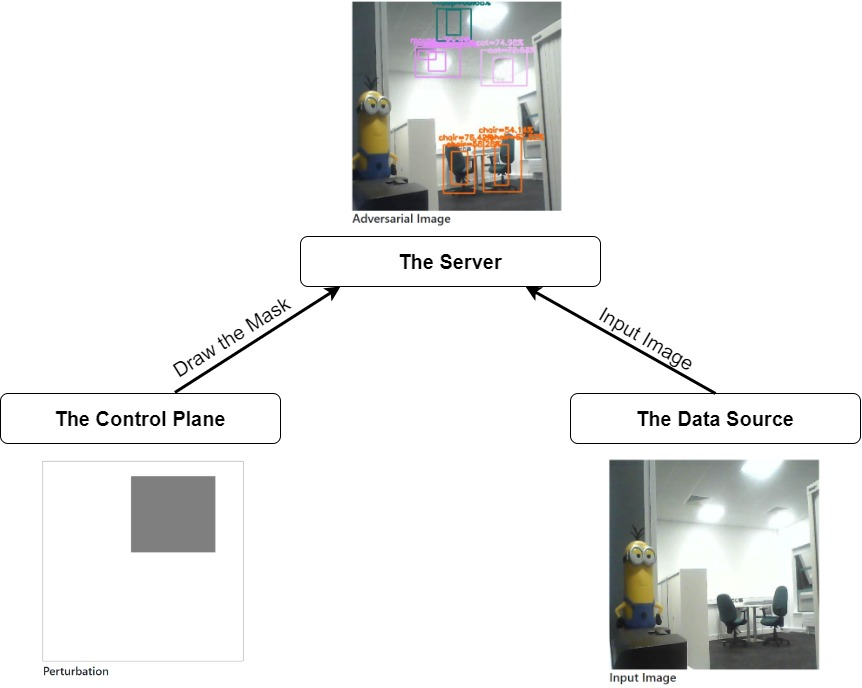
\includegraphics[width=0.48\textwidth]{figures/chapter_detection/structure.jpg}
%     \caption{Adversarial Detection: System Architecture}
%     \label{fig:architecture}
% \end{figure}

\subsection{System Architecture}

To attack the YOLO object detection model, the adversarial detection system adopts a modular design pattern so that we can test our attacks in different environments (see Fig. \ref{fig.adv_detect_demo}) using the same architecture. The system consists of three components: the Data Source, the Server, and the Control Panel.

% We present our experimental results in the next section.

\begin{figure}[H]
\centering
\begin{subfigure}[b]{\textwidth}
    \centering
    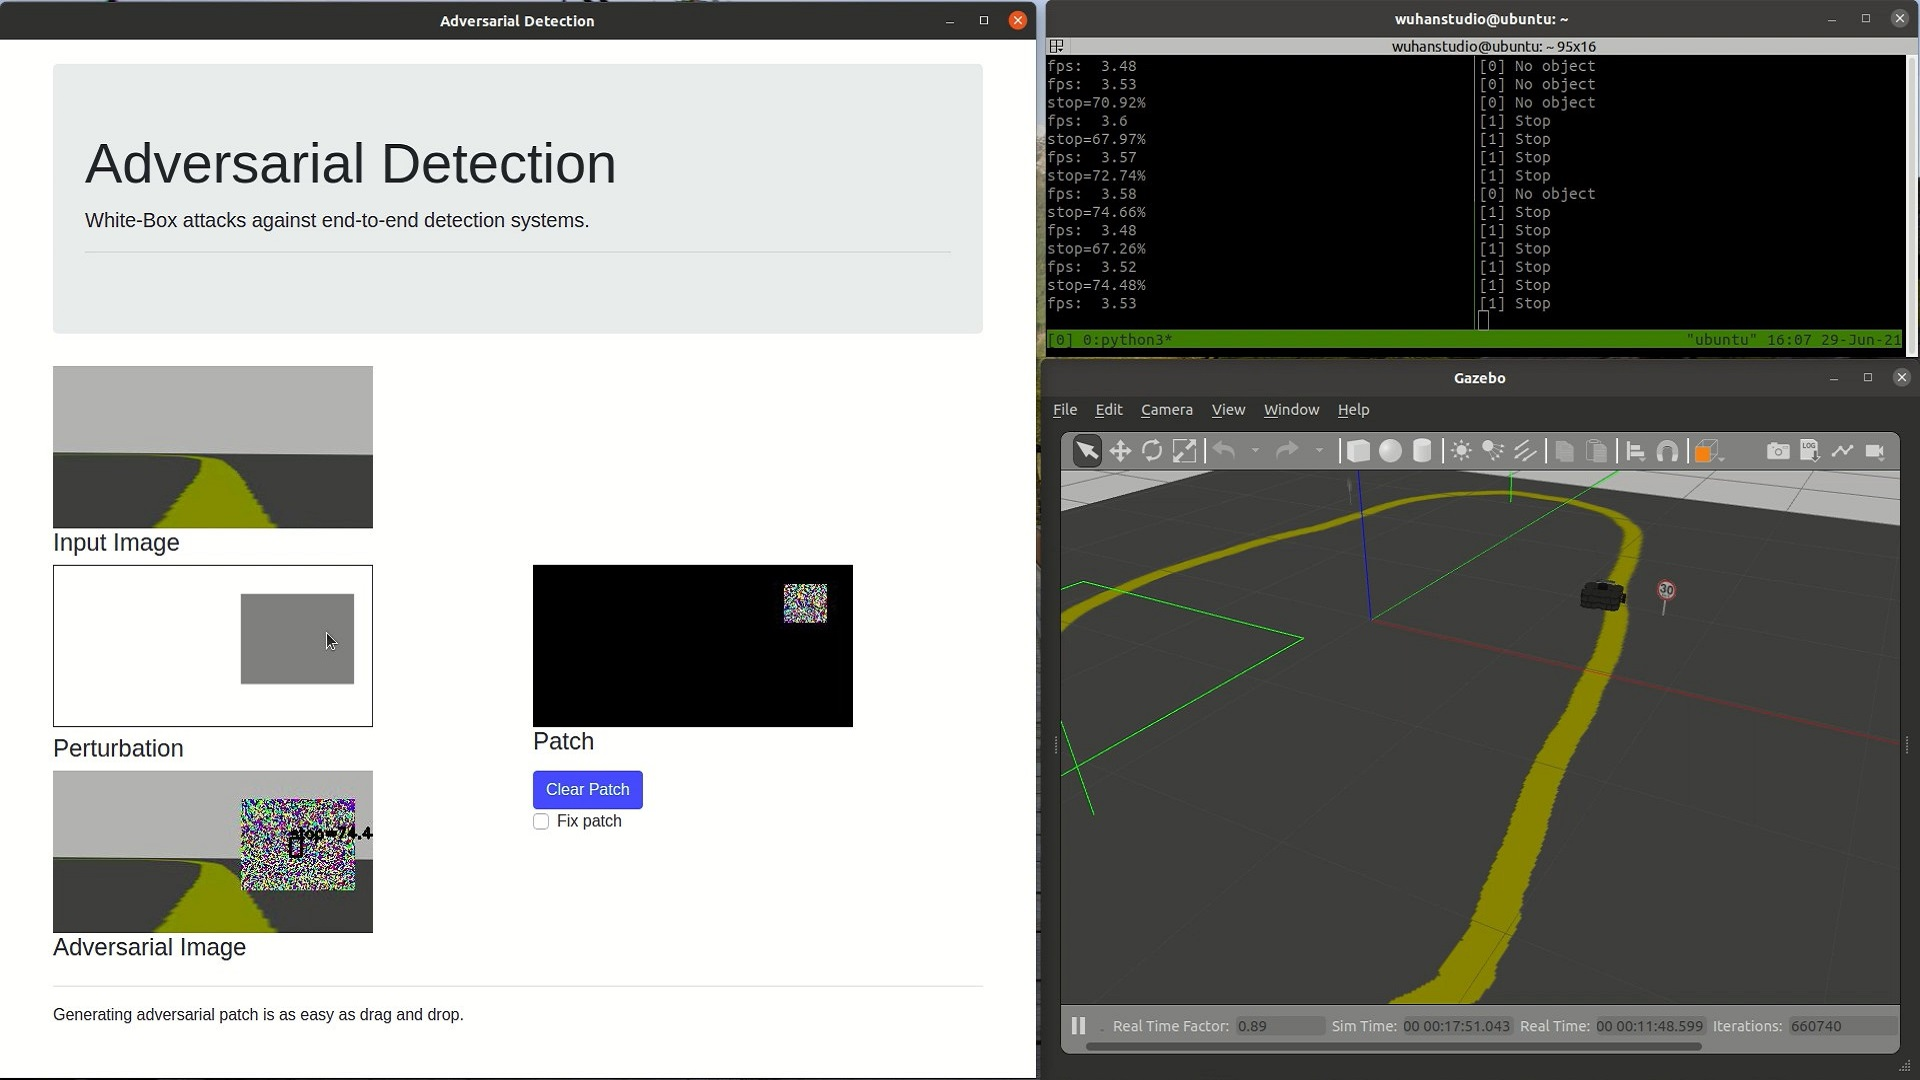
\includegraphics[width=\textwidth]{figures/chapter_detection/detection/gazebo.jpg}
    \caption{The Adversarial Overlay in Gazebo.}
    \label{fig:gazebo}
\end{subfigure}
\begin{subfigure}[b]{\textwidth}
    \centering
    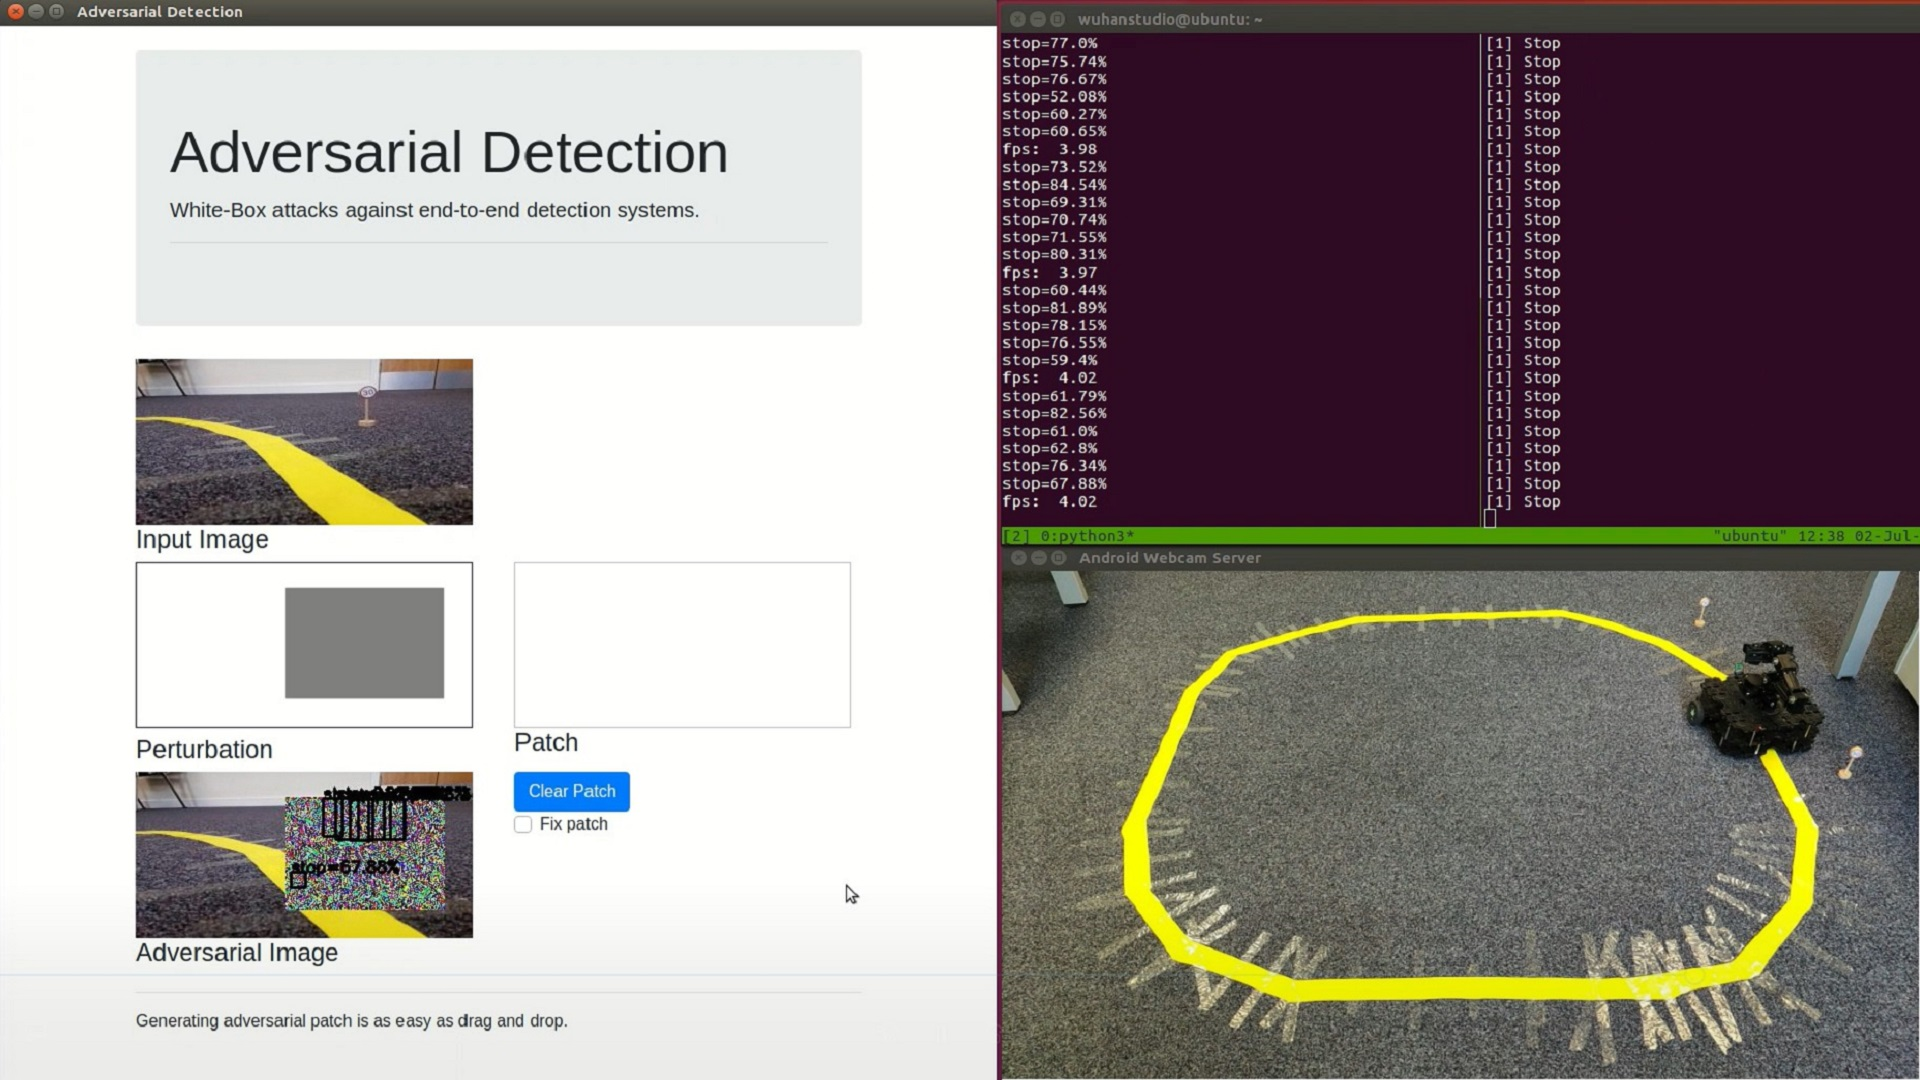
\includegraphics[width=\textwidth]{figures/chapter_detection/detection/turtlebot.jpg}
    \caption{The Adversarial Overlay on Turtlebot3.}
    \label{fig:turtlebot}
\end{subfigure}
\end{figure}
\begin{figure}[H]\ContinuedFloat
\centering
\begin{subfigure}[b]{\textwidth}
    \centering
    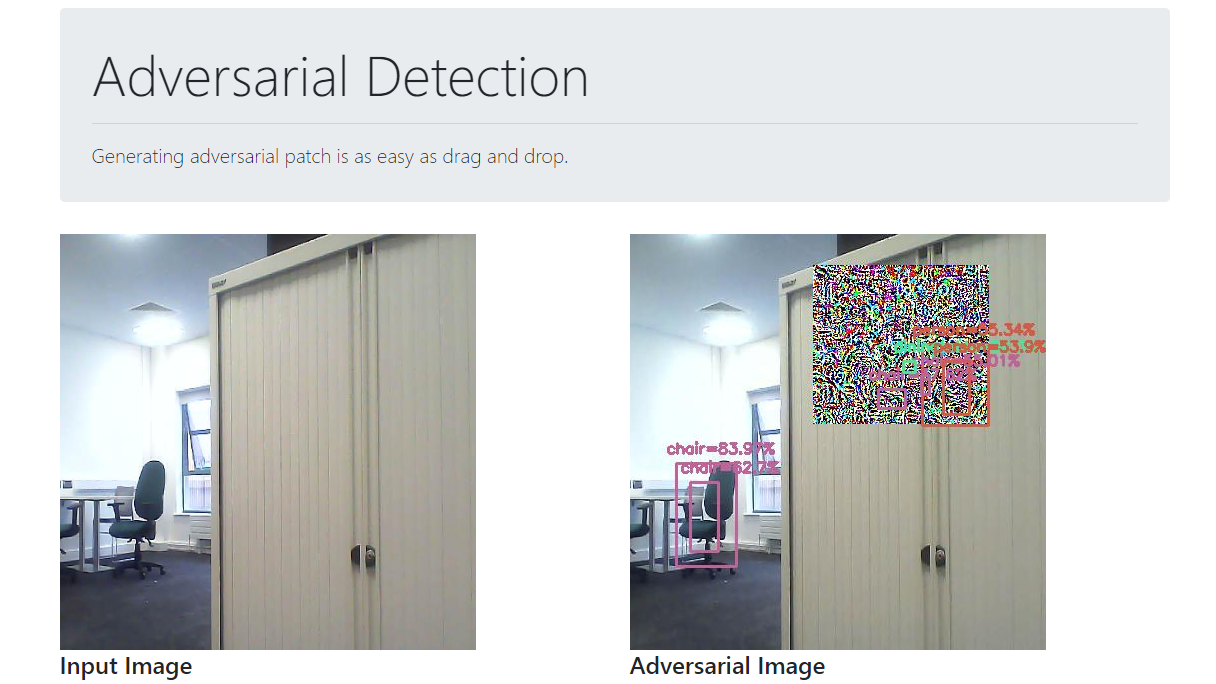
\includegraphics[width=\textwidth]{figures/chapter_detection/detection/pc.png}
    \caption{The Adversarial Overlay on a Laptop.}
    \label{fig:pc}
\end{subfigure}
\caption{We tested our attack in three environments. Here we made the overlay visible for illustration purposes.}
\label{fig.adv_detect_demo}
\end{figure}

\textbf{The Data Source}: The data source publishes the input image to the server. We can publish the image from different sources, including a PC camera, the ROS Gazebo Simulator, and a real Turtlebot 3.

\textbf{The Server}: The server receives the input image stream from the data source via WebSocket connections. Meanwhile, it obtains the adversarial mask from the control plane. The server then generates and injects the adversarial overlay into the input image. In addition, the YOLO object detection model is deployed on the server.

\textbf{The Control Plane}: The control plane is a website where the attacker can draw the mask at arbitrary locations. Then, the browser sends the mask to the server via Websocket connections.

\subsection{Experimental Results}

We used YOLO object detection models pre-trained on the MS COCO dataset for the PC environment. Moreover, we trained two traffic sign detection models using YOLO for the ROS Gazebo and the ROS Turtlebot environment. 

\subsubsection{Evaluation Metrics}

Prior research have used the Mean Average Precision (mAP) \citep{cartucho2018} to evaluate the accuracy of object detection models. However, the objective of our attack is to fabricate new bounding boxes, not to decrease the accuracy of existing objects. Therefore, the evaluation metrics need to reflect the efficiency of generating new bounding boxes in real time, something which mAP cannot do. In addition, the mAP evaluation metric requires access to the ground truth, that is, human-labeled bounding boxes. The online attack that fools the object detection system in real time does not have any such ground truth since it is impossible for humans to label the video stream in real time. Thus, we use the following two evaluation metrics that evaluate the efficiency of generating new objects and do not require ground truth labels.

\textbf{Success Rate}: The success rate measures the percentage of images we successfully fabricate at least one object within a limited number iterations. For a real-time online attack, we need to achieve a satisfying success rate within a limited number of iterations.

\textbf{Mean Box Number Increase}: We measure the number of new bounding boxes generated compared to the benign output. The more bounding boxes we generate, the stronger the perturbation is. However, to fabricate more objects we also need a larger number of iterations.

In general, we will attempt to find the minimum number of iterations required to achieve a satisfying success rate and fabricate enough bounding boxes. The PASCAL VOC-2012 validation set is used in the following experiments.

\subsubsection{Hyper-parameters}
\label{sec:hyper}

Three hyper-parameters are crucial for the attack: the attack strength $\xi$, the step size $\alpha$, and the box size. For monochrome overlays, we investigated the effect of using gradients from different channels. In addition, we examined if the adversarial perturbation is sensitive to the aspect ratio.

\textbf{The Attack Strength}: The attack strength $\xi$ sets a boundary on the maximum perturbation added to each pixel. A larger $\xi$ makes the attack stronger but also results in a more conspicuous perturbation. In Fig. \ref{fig:xi_suc}, $\xi \in \{8, 10\}$ results in a much higher success rates than $\xi \in \{2, 4\}$ after 100 iterations. Though $\xi=8$ and $\xi=10$ share similar success rates, $\xi=10$ generates more bounding boxes than $\xi=8$ (see Fig. \ref{fig:xi_box}). For a real-time attack, we aim to generate at least one bounding box in 30 iterations, a requirement which is satisfied with both $\xi=8$ and $\xi=10$. $\xi=8$, in particular, finds a good balance between the attack strength and the impermeability of the perturbation.

\textbf{The Step Size}: The step size $\alpha$ controls how fast we update the perturbation in each iteration. A larger $\alpha$ would make it possible to fabricate bounding boxes in fewer iterations but make the update more unstable. In Fig. \ref{fig:alpha_suc}, both $\alpha=1$ and $\alpha=2$ achieve a success rate of more than 90\% after just 30 iterations, whereas $\alpha > 4$ produces a worse the success rate. In Fig. \ref{fig:alpha_box}, though $\alpha=1$ eventually generates more bounding boxes than $\alpha=2$, it is preferable to have a faster attack.

\textbf{The Box Size}: The box size determines the total number of pixels we can perturb. The more pixels we can manipulate, the easier it is to deviate the model output. We need to find the minimum box size for our attack. In Fig. \ref{fig:box_suc}, the box sizes of both 64x64 and 128x128 achieve a success rate of 90\% after just 30 iterations, while the box size of 32x32 struggles to achieve successful attacks. Moreover, with box size smaller than 16x16 we are unable to attack the model with $\xi=8$ and $\alpha=2$. In addition, as expected, the larger the box size is, the more bounding boxes the attack can generate (see Fig. \ref{fig:box_box}). For a real-time online attack, we suggest the overlay box size to be at least 64x64.

\begin{figure}[H]
    \centering
    \begin{subfigure}[b]{0.5\textwidth}
        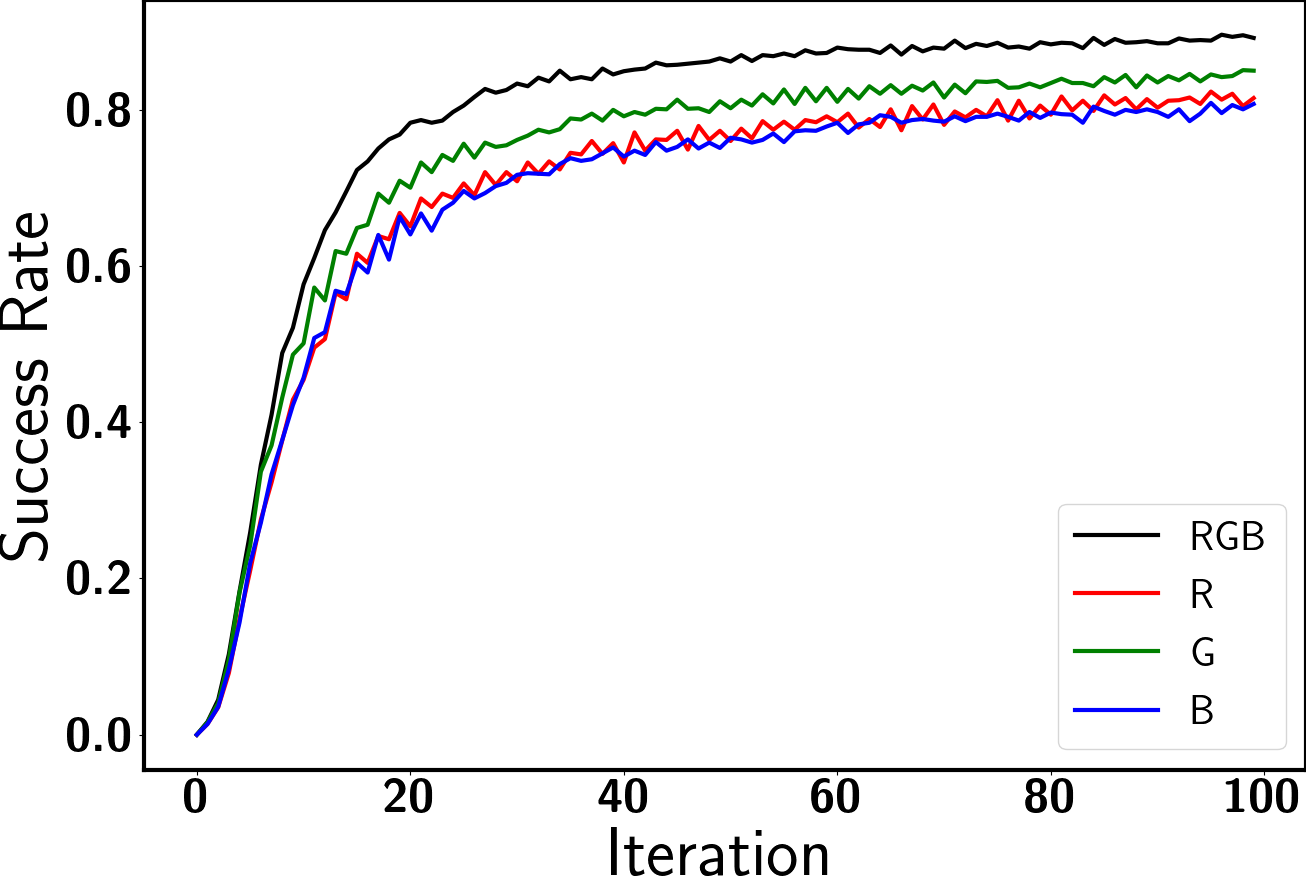
\includegraphics[width=\textwidth]{figures/chapter_detection/detection/multi_untargeted_mono_success.png}
        \caption{Different channels (Red, Green, Blue).}
         \label{fig:mono_suc}
    \end{subfigure}
    \begin{subfigure}[b]{0.9\textwidth}
        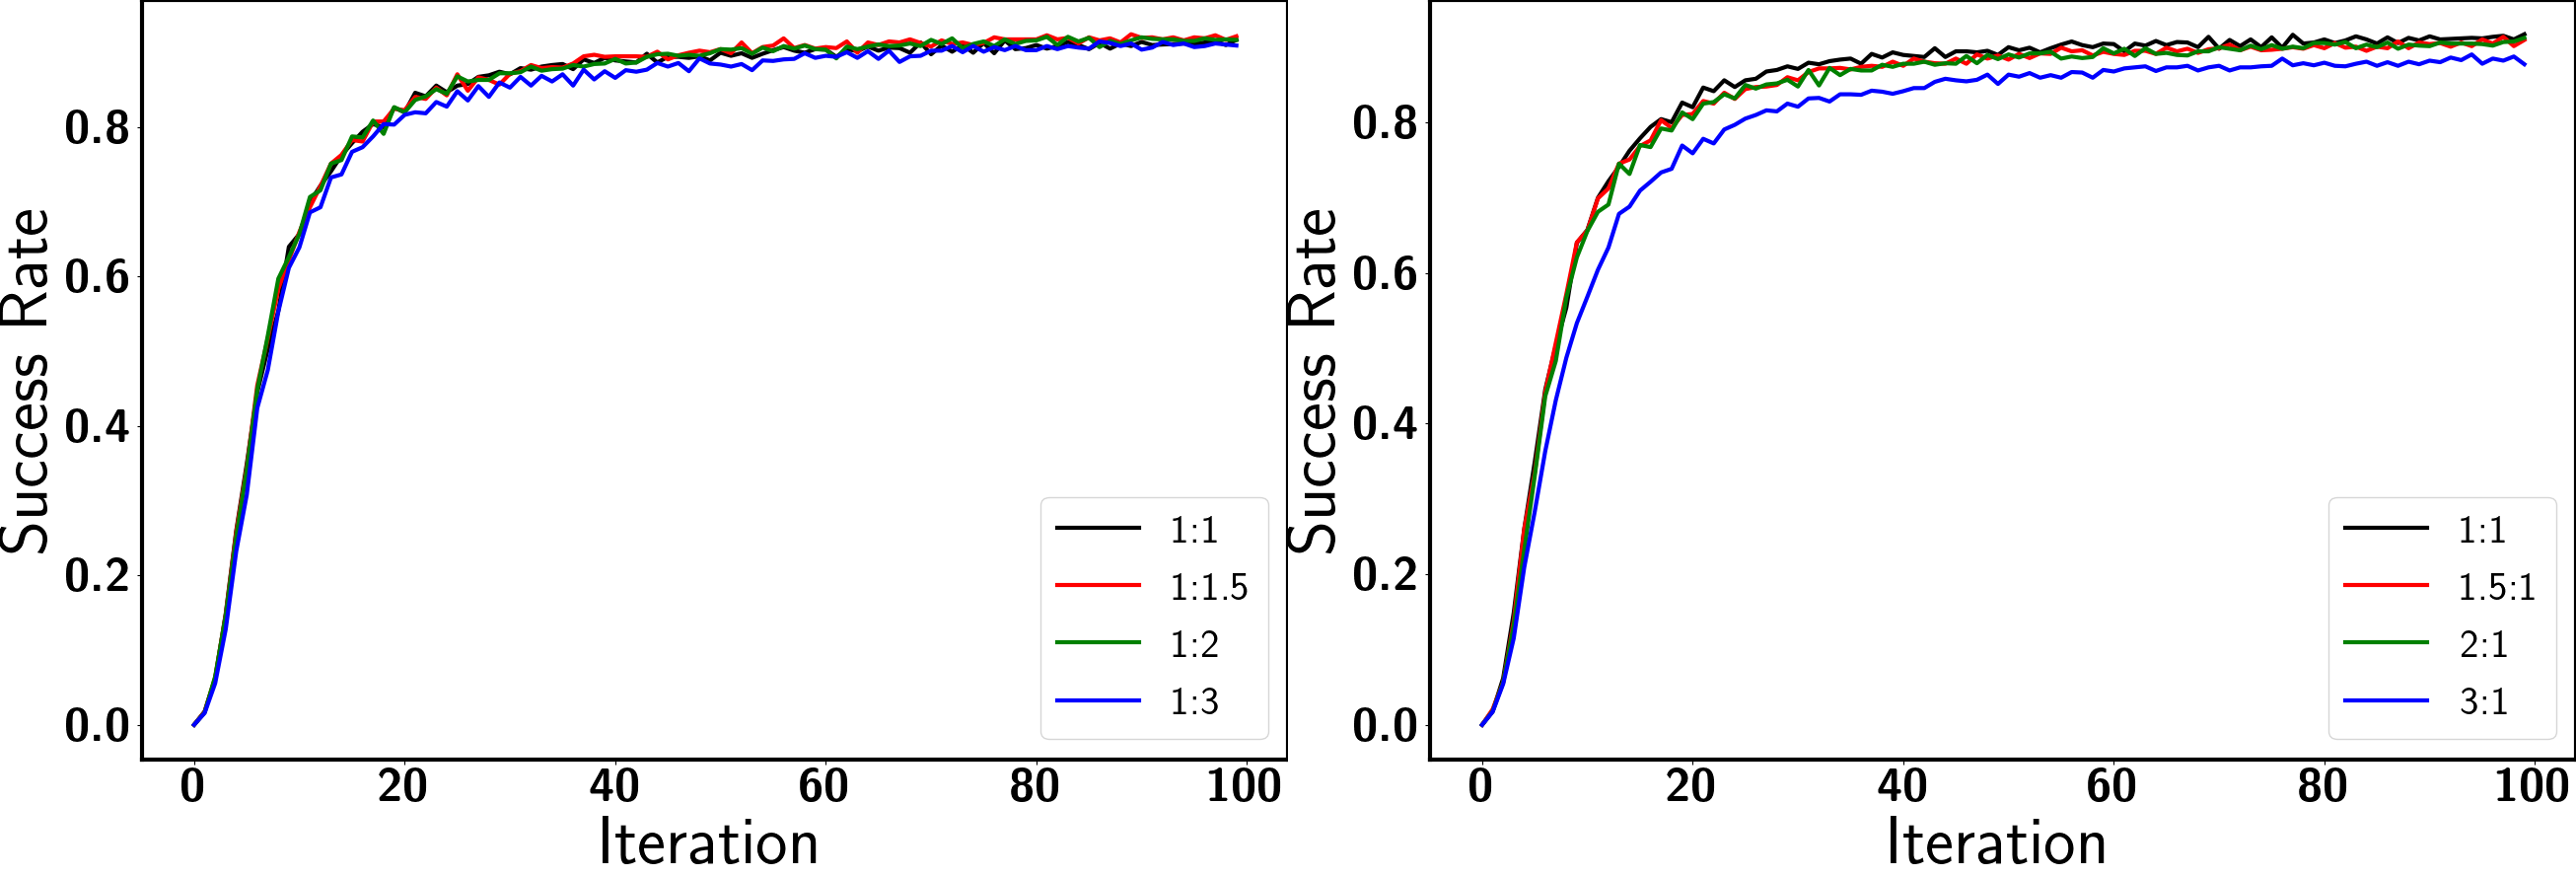
\includegraphics[width=\textwidth]{figures/chapter_detection/detection/multi_untargeted_aspect_success.png}
        \caption{Different aspect ratios (left $1:n$, right: $n:1$).}
         \label{fig:aspect_suc}
    \end{subfigure}
    \caption{The success rate of the multi-untargeted attack with different channels and aspect ratios.}
\end{figure}

\begin{figure}[H]
    \centering
    \begin{subfigure}[b]{0.5\textwidth}
        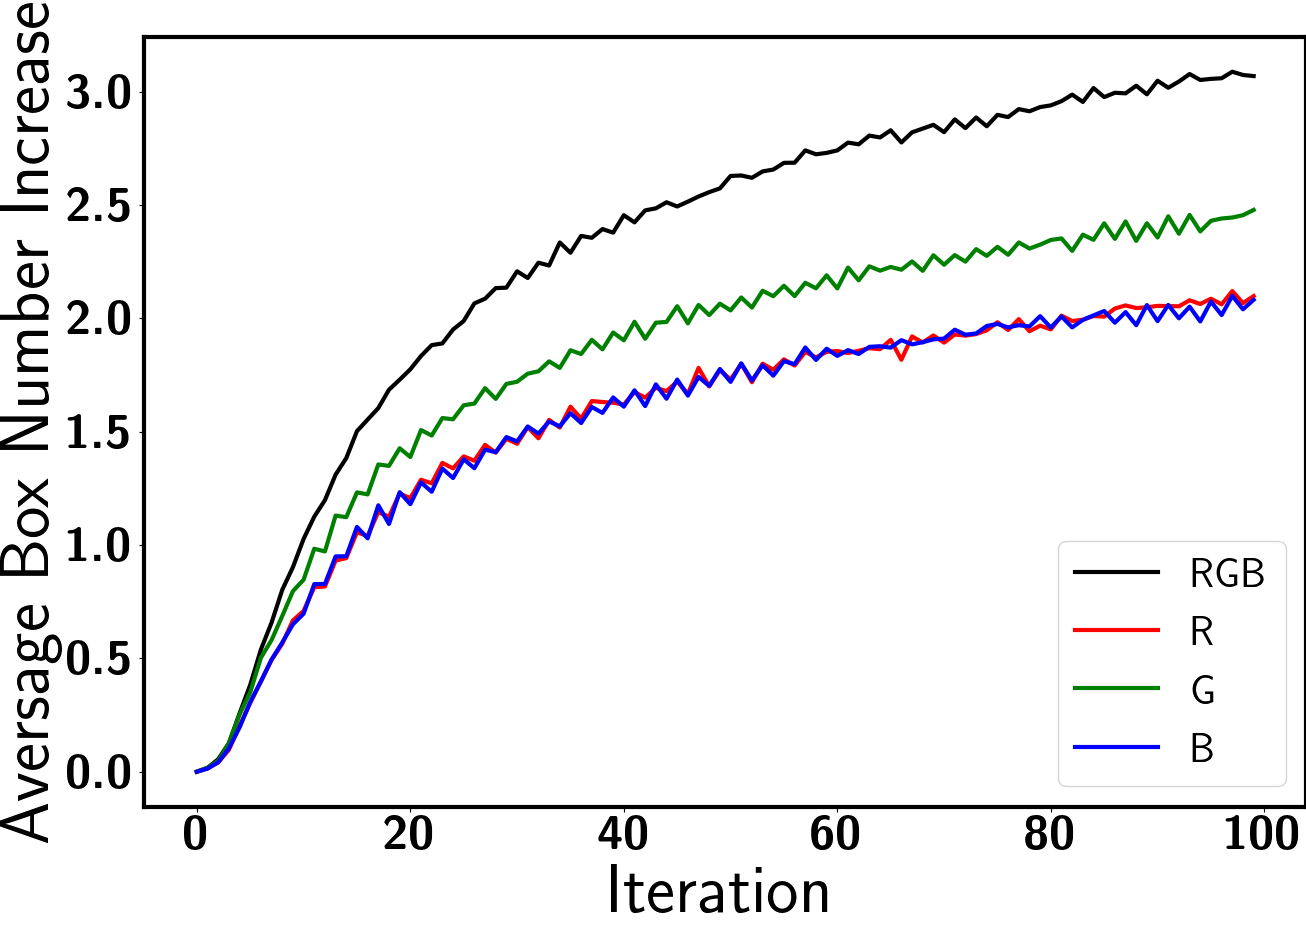
\includegraphics[width=\textwidth]{figures/chapter_detection/detection/multi_untargeted_mono_box.png}
        \caption{Different channels (Red, Green, Blue).}
         \label{fig:mono_box}
    \end{subfigure}
    \begin{subfigure}[b]{0.9\textwidth}
        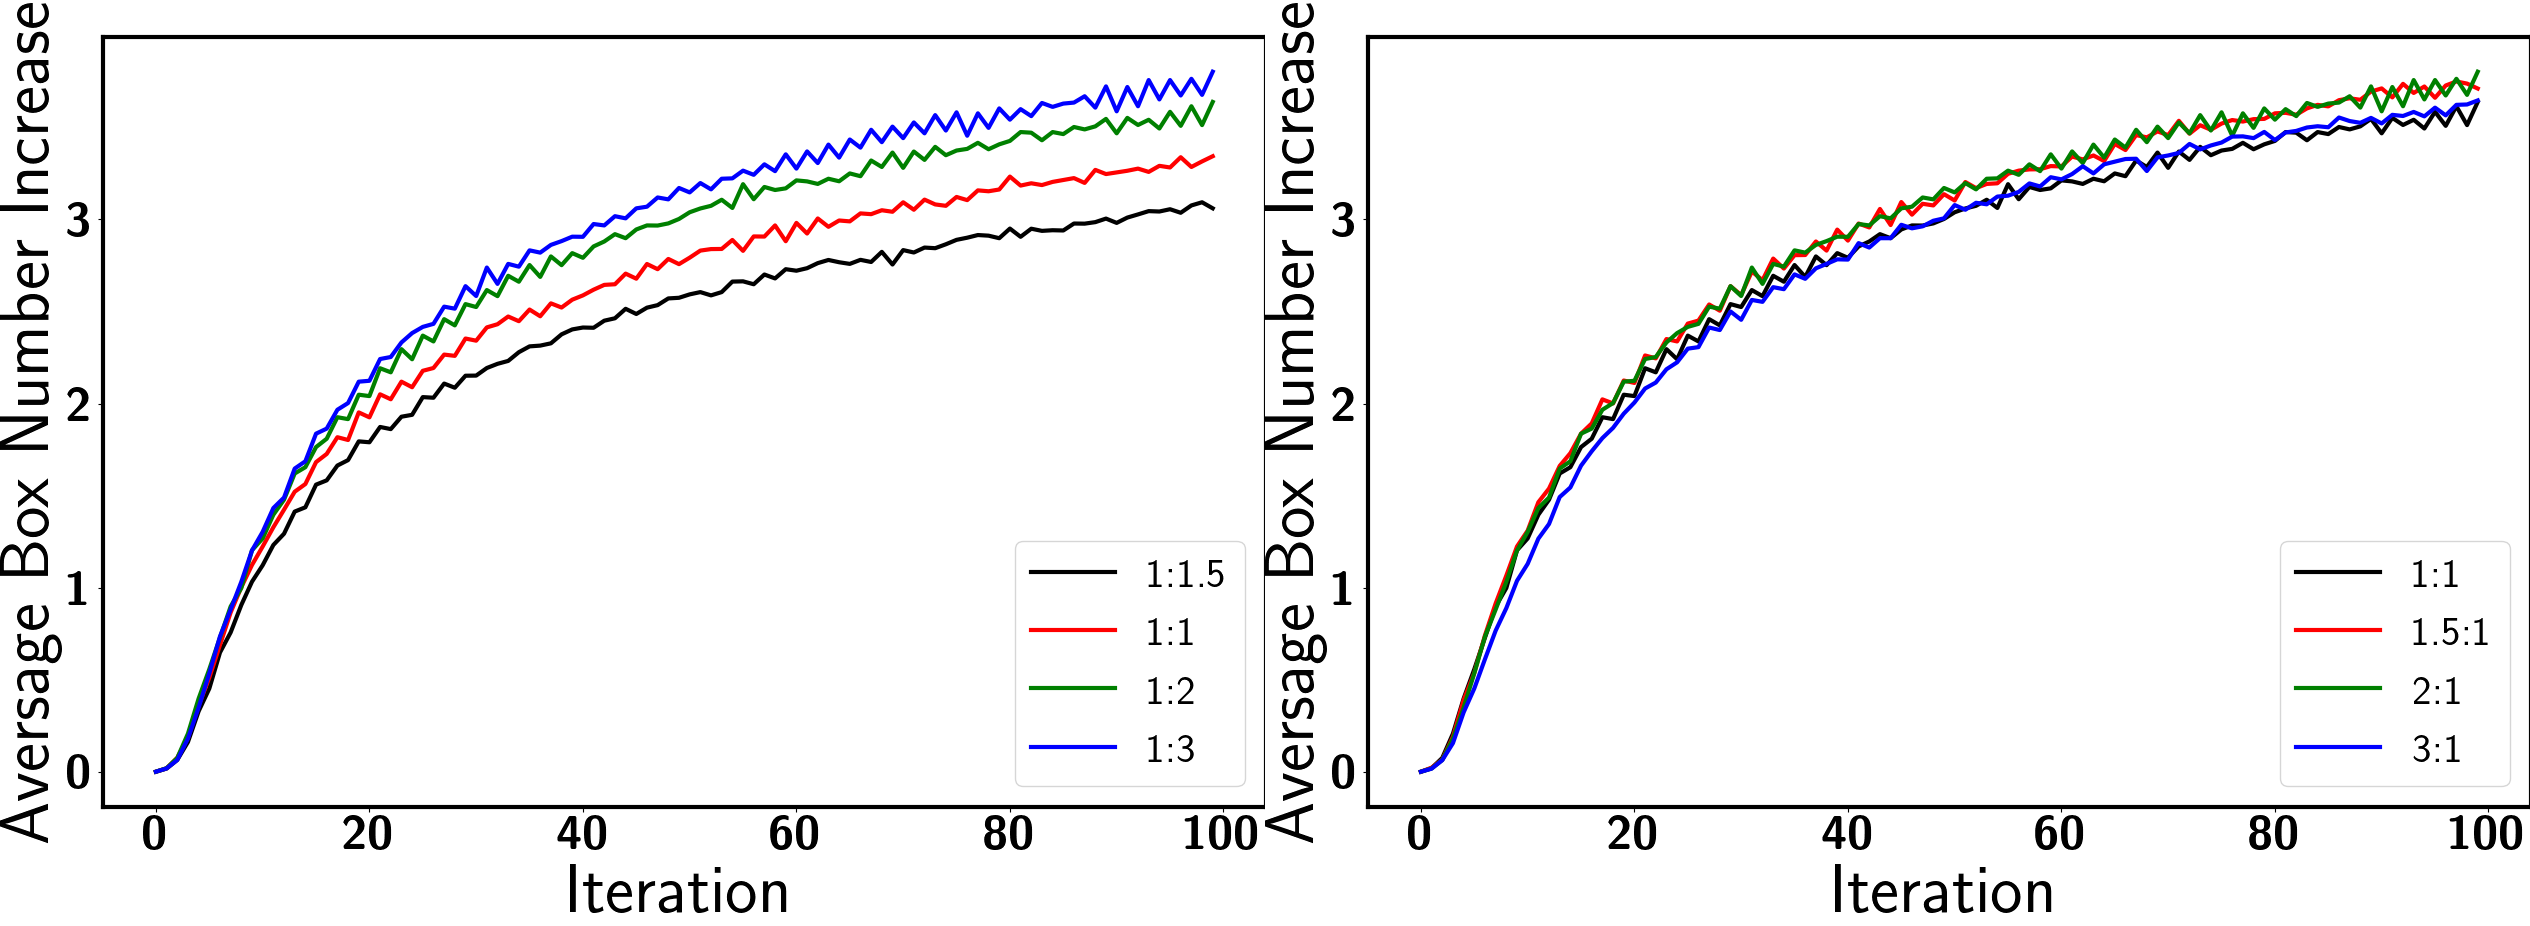
\includegraphics[width=1\textwidth]{figures/chapter_detection/detection/multi_untargeted_aspect_box.png}
        \caption{Different aspect ratios (left $1:n$, right: $n:1$).}
         \label{fig:aspect_box}
    \end{subfigure}

    \caption{The average box number increase of the multi-untargeted attack different channels and aspect ratios.}
\end{figure}

\textbf{The Monochrome Channel}: For the attack that generates a polychrome overlay, we update each channel of the perturbation using the gradients of each channel. While for the monochrome overlay, we decide which color channel to prioritize. Interestingly, the experimental results (see Fig. \ref{fig:mono_suc} and Fig. \ref{fig:mono_box}) show that the object detection model is the most sensitive to the green channel. Using the average gradient of RGB channels, we achieve the highest success rate and generate the most number of boxes.

\textbf{The Aspect Ratio}: Our attack can generate adversarial overlays of arbitrary shapes. Thus, we can study if the object detection model is more susceptible to adversarial overlays of specific aspect ratios, e.g., wide (1:n) or long (n:1) boxes. For a fair comparison, overlay boxes of different aspect ratios have the same number of pixels perturbed. In Fig. \ref{fig:aspect_suc}, different aspect ratios do not cause observable dissimilarities in success rates. Although the aspect ratio $1:3$ generates more bounding boxes than $1:1.5$ after 100 iterations (see Fig. \ref{fig:aspect_box}), this attributes to a slightly more number of boxes perturbed ($1:3 \rightarrow 37 \times 111 = 4108$, $1:1.5 \rightarrow 52 \times 78 = 4056$). Thus, we cannot conclude that the aspect ratio has any discernible impact on the attack. As a result, we use $\xi=8$, $\alpha=2$, and a box size of 64x64 as default values for our attack, and the monochrome overlay uses the average of gradients from RGB channels.

\subsubsection{The Attack Performance}

We measured the performance of the attack on an NVIDIA RTX 2080Ti GPU. According to prior experimental results, we chose the hyper-parameters of $\xi=8$, $\alpha=2$, and used the box sizes of 64x64 and 128x128. Then, we tested the attack on the VOC 2012 validation set, which includes 5823 images in total (see Table \ref{tab:fix-it} and \ref{tab:fix-box}).

% \addtolength{\textheight}{-2cm}

% \clearpage

In Table \ref{tab:fix-it}, the attack achieved 24 FPS (1 iteration cost 41 ms). It should be noted that the performance of the attack also depends on model size. A larger model requires more computations to compute the gradient. Besides, the time cost does not grow as the box size increases (64 x 64 and 128 x 128) since we calculate the gradient of the adversarial loss functions over the entire input image, making it possible to generate multiple overlays of different shapes simultaneously without recalculating gradients.

\begin{table}[H]
    \centering
    \begin{tabular}{cccc}
    \hline
    Box Sizes & 1 iteration & 10 iterations & 20 iterations\\
    \hline
    \ 64x64    & 41 ms  & 410 ms & 780 ms \\
    \ 128x128  & 41 ms  & 410 ms & 781 ms \\
    \hline
    \end{tabular}
    \caption{The time cost of the attack with different numbers of iterations ($\alpha=2,\ \xi=8$).}
    \label{tab:fix-it}
\end{table}

\begin{table}[H]
    \centering
    \begin{tabular}{cccc}
    \hline
    Box Sizes & N=1 & N=3 & N=5\\
    \hline
    \ 64x64    & 7.47 it (306 ms)  & 12.03 it (493 ms) &  13.62 it (558 ms)) \\
    \ 128x128  & 4.40 it (180 ms)  & 7.64 it (313 ms) & 10.20 it (418 ms) \\
    \hline
    \end{tabular}
    \caption{The average number of iterations and time cost of generating N bounding boxes ($\alpha=2,\ \xi=8$).}
    \label{tab:fix-box}
\end{table}

As illustrated in Table \ref{tab:fix-box}, on average, the attack requires only 7 iterations within around 300 ms to generate one bounding box for each static image (offline attack). 

For an online attack, the attack can be even more efficient. It is unnecessary to re-generate the adversarial overlay from scratch for every input video frame since there is a high correlation between consecutive video frames and iterations \citep{ilyas2018prior}. As a result, we can save computations by reusing the overlay generated in the previous timestep. In the demo video, the attack achieved near real-time performance on an Intel i7-8665U CPU.

\clearpage

\null
\vfill

\begin{figure}[H]
\centering
\begin{subfigure}[b]{0.60\textwidth}
    \centering
    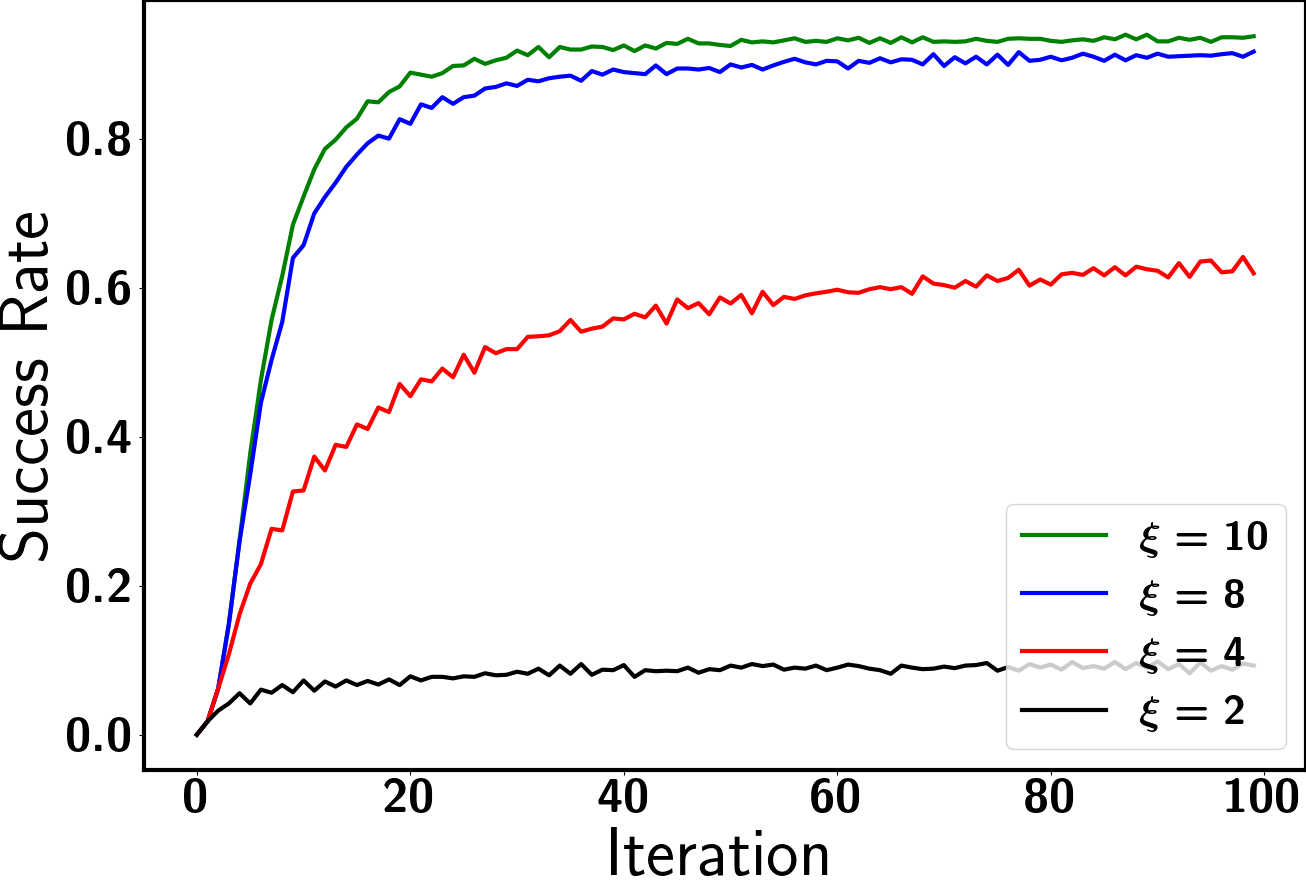
\includegraphics[width=\textwidth]{figures/chapter_detection/detection/multi_untargeted_xi_success.png}
    \caption{Different $\xi$ with $\alpha=2$, box size$=64$.}
    \label{fig:xi_suc}
\end{subfigure}
\hfill
\begin{subfigure}[b]{0.60\textwidth}
    \centering
    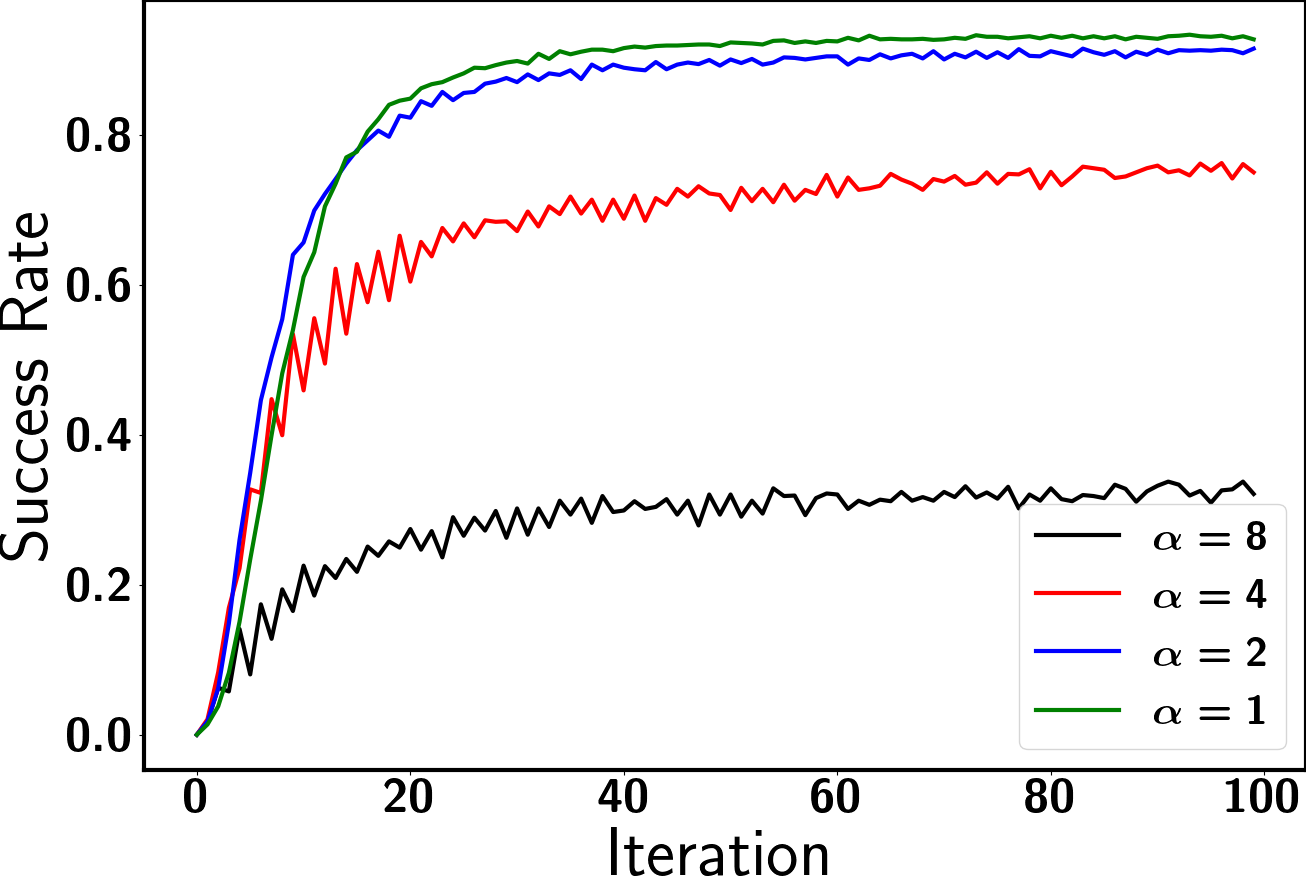
\includegraphics[width=\textwidth]{figures/chapter_detection/detection/multi_untargeted_lr_success.png}
    \caption{Different $\alpha$ with $\xi=8$, box size $=64$.}
    \label{fig:alpha_suc}
\end{subfigure}
\hfill
\begin{subfigure}[b]{0.60\textwidth}
    \centering
    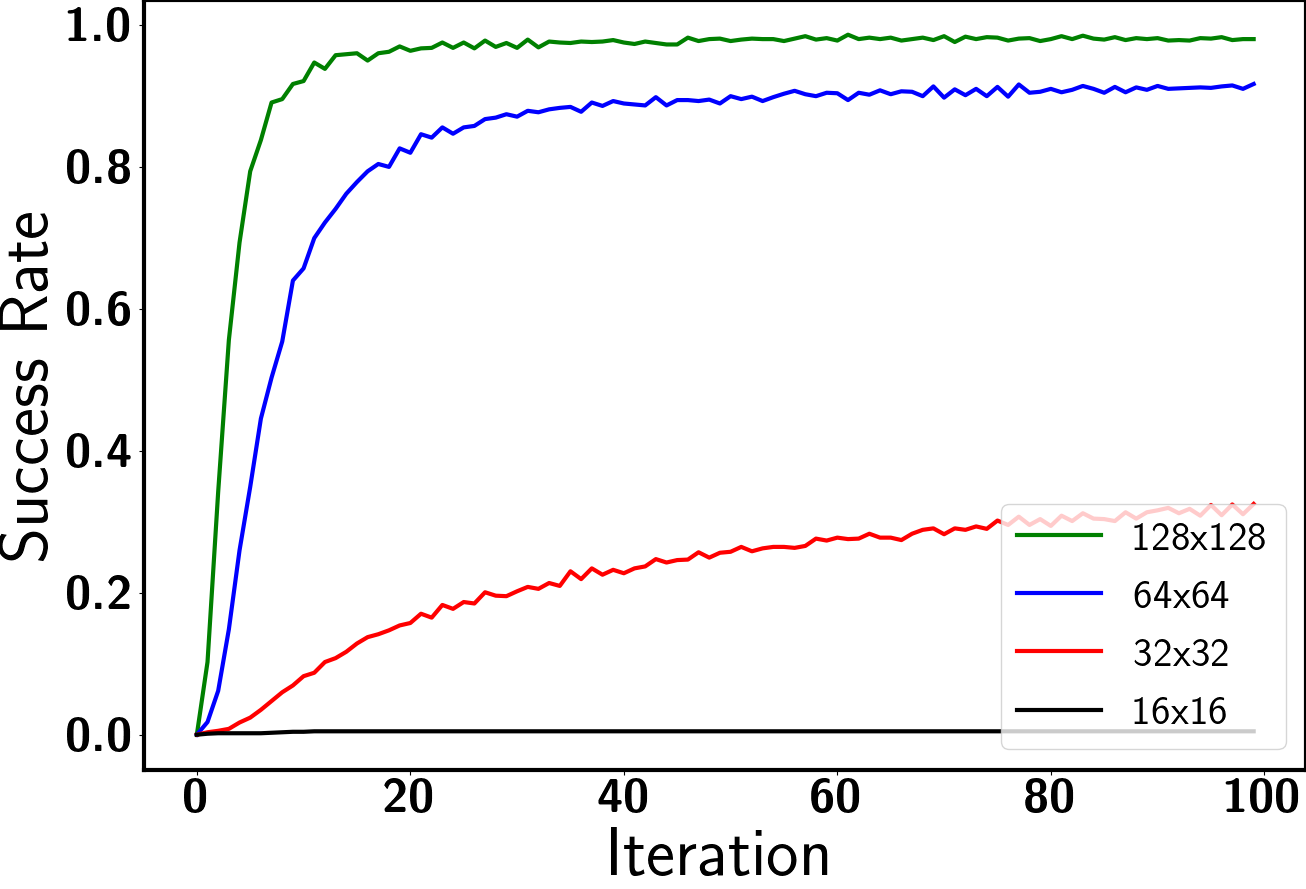
\includegraphics[width=\textwidth]{figures/chapter_detection/detection/multi_untargeted_box_success.png}
    \caption{Different box sizes with $\xi=8, \alpha=2$.}
    \label{fig:box_suc}
\end{subfigure}
\caption{The success rate of the multi-untargeted attack with different $\xi$, $\alpha$, and box sizes.}
\label{fig.hyper_suc}
\end{figure}

\vfill

\clearpage

\null
\vfill

\begin{figure}[H]
\centering
\begin{subfigure}[b]{0.59\textwidth}
    \centering
    \includegraphics[width=\textwidth]{figures/chapter_detection/detection/multi_untargeted_xi_box.png}
    \caption{Different $\xi$ with $\alpha=2$, box size$=64$.}
    \label{fig:xi_box}
\end{subfigure}
\hfill
\begin{subfigure}[b]{0.59\textwidth}
    \centering
    \includegraphics[width=\textwidth]{figures/chapter_detection/detection/multi_untargeted_lr_box.png}
    \caption{Different $\alpha$ with $\xi=8$, box size $=64$.}
    \label{fig:alpha_box}
\end{subfigure}
\hfill
\begin{subfigure}[b]{0.59\textwidth}
    \centering
    \includegraphics[width=\textwidth]{figures/chapter_detection/detection/multi_untargeted_box_box.png}
    \caption{Different box sizes with $\xi=8, \alpha=2$.}
    \label{fig:box_box}
\end{subfigure}
\caption{The average box number increase of the multi-untargeted attack with different $\xi$, $\alpha$, and box sizes}
\label{fig.hyper_box}
\end{figure}

\vfill

\clearpage

\subsection{Conclusions}

This research demonstrates that it is possible to attack an object detection system in real time. We generate human unperceivable adversarial overlays of arbitrary shapes to fabricate bounding boxes at desired locations. This attack could be a threat to the areas of traffic sign recognition and the autonomous driving field as a whole.

In the future, we plan to investigate the effect of the attack on modular autonomous driving systems that rely on object detection models to perceive the environment. In addition, we will explore how to detect adversarial attacks so that we can embrace deep learning models in safety-critical robotic applications in a safe way.

% \clearpage

\section{The Human-in-the-Middle Attack}

The last section introduces how we generate and apply digital patches in ROS. This attack requires access to ROS topics and online gradients, which means different perturbations are computed at different time steps. Can we generate a single universal perturbation that attacks all the frames, and is it possible to attack an object detection system without access to the internal system? 

% To solve this problem, we devise the Man-in-the-Middle Attack. The idea of the Man-in-the-Middle attack is borrowed from cryptography,  in which the attacker makes independent connections with the victims and relays messages between them to make them believe they are talking directly to each other over a private connection, but in fact, the entire conversation is controlled by the attacker. Similarly, we attack the detection system by tampering with the image data between the sensor and the operating system. The operating system where detection models are deployed is usually highly secure, but we notice that the sensor (camera) that captures the image is exposed directly to the outside world without any protection. If we add the perturbation to the sensor, rather than into the detection system, we can achieve practical digital attacks without access to the internal system. 

% \begin{abstract}
Object detection systems using deep learning models have become increasingly popular in robotics thanks to the rising power of CPUs and GPUs in embedded systems. However, these models are susceptible to adversarial attacks. While some attacks are limited by strict assumptions on access to the detection system, we propose a novel hardware attack inspired by Man-in-the-Middle attacks in cryptography. This attack generates a \acrfull{uap} and injects the perturbation between the USB camera and the detection system via a hardware attack. Besides, prior research is misled by an evaluation metric that measures the model accuracy rather than the attack performance. In combination with our proposed evaluation metrics, we significantly increased  the strength of adversarial perturbations. These findings raise serious concerns for applications of deep learning models in safety-critical systems, such as autonomous driving.
% \end{abstract}

% \begin{IEEEImpStatement}
% Advancements in deep neural networks have ushered in a new era of robotics, characterized by intelligent robots with a comprehensive understanding of the environment, thanks to deep learning models. However, it is no more a secret that deep learning models are vulnerable to adversarial attacks. Besides existing digital and physical attacks, we introduce a novel 'Human-in-the-Middle' hardware attack that injects digital perturbation into the physical sensor. Our research opens up new possibilities for adversarial attacks, and we hope to embrace deep learning models securely for robotic applications.

% It is no more a secret that deep learning models are vulnerable to adversarial attacks. However, how to apply adversarial perturbations practically remains an open challenge. Digital attacks that inject perturbations into the input image can be challenging due to the lack of access to the internal system. Physical attacks that print perturbations on physical objects, such as posters, are sensitive to position and angle variations. Our novel man-in-the-middle hardware attack injects digital perturbation into the physical sensor, opening up new possibilities for applying adversarial attacks. 

% \end{IEEEImpStatement}

% \begin{IEEEkeywords}
% Adversarial Attacks, Object Detection, 
% Deep Learning.
% \end{IEEEkeywords}

\subsection{Introduction}

The development of deep neural networks has enabled the creation of intelligent robots that possess a more comprehensive perception of the environment than traditional robots. However, this shift towards intelligent robots has also brought with it an increasing risk of adversarial attacks, especially in safety-critical applications.  It has been a decade since the existence of adversarial examples was first identified by Biggio et al. \citep{biggio2013evasion}, and Szegedy et al. \citep{szegedy2013intriguing}, in which they fooled an image classification model by adding a small perturbation to the input image.  Although the perturbation was imperceptible to humans, it caused the deep learning model to produce erroneous classification results. The attack was later extended from classification models to detection models \citep{han2023detection, LuSFF17}. 

%Despite substantial research efforts to understand adversarial attacks, it is still unclear how they could affect real-world systems, such as object detection models deployed in autonomous driving systems.  

Adversarial attacks against deep learning models can be divided into two categories: digital attacks and physical attacks. Digital attacks directly apply perturbations to the digital input image by modifying pixel values \citep{han2023driving}, while physical attacks involve printing the perturbation on physical objects such as posters \citep{lee2019physical} or T-shirts \citep{xu2020adversarial}.

However, both digital and physical attacks have their limitations. Digital perturbation requires access to the detection system, making it difficult to apply in real-world scenarios such as hacking into a self-driving car. Physical attacks, on the other hand, are sensitive to position and angle variations. For instance, experiments in \citep{LuSFF17} showed that an autonomous vehicle only misclassified traffic signs placed within 0.5 meters of the camera and viewed from specific angles. Moreover, these attacks lack flexibility, as once the adversarial object is printed, it can only be changed through reprinting. The trial-and-error process of finding a successful attack object can take a long time and require significant amounts of printing.

\subsection{Contributions}

This paper presents a novel hardware attack that combines the flexibility of physical attacks with the efficiency of digital attacks, inspired by Man-in-the-Middle Attacks in network security (refer to Fig. \ref{fig:mitm}). In this attack, the adversary intercepts and manipulates the image data transmitted between a USB camera and a detection system (refer to Figs. \ref{fig:minm} and \ref{fig:demo}). 

The key contributions of this research are summarized as follows:

\begin{enumerate}
    \item We present a novel hardware attack, called Human-in-the-Middle  attack, that offers both efficiency and ease of deployment for adversarial attacks\footnote{The source code of the hardware attack is available on GitHub: \url{https://github.com/wuhanstudio/adversarial-camera}}. By utilizing learning rate decay during the generation of the perturbation, our attack is capable of generating more bounding boxes than competing attack methods.
    \item We introduce three new evaluation metrics that offer a more nuanced approach to evaluating adversarial attacks. Unlike existing metrics that make a binary decision for each bounding box, our metrics consider the confidence value and probability vector in a linear fashion.
    \item We devise and open source the white-box adversarial toolbox\footnote{The source code of the toolbox is available on GitHub: \url{https://github.com/wuhanstudio/whitebox-adversarial-toolbox}} that simplifies the process of generating adversarial perturbations. The toolbox focuses on real-time white-box attacks against object detection models.
\end{enumerate}

% \clearpage

\begin{figure}[H]
    \centering
    \begin{subfigure}[b]{\textwidth}
        \includegraphics[width=\textwidth]{figures/chapter_detection/hardware/mitm.png}
        \caption{Man-in-the-Middle Attack in Network Security}
        \label{fig:mitm} 
    \end{subfigure}

    \begin{subfigure}[b]{\textwidth}
        \includegraphics[width=\textwidth]{figures/chapter_detection/hardware/overview.png}
        \caption{Human-in-the-Middle Attack in Deep Learning}
        \label{fig:minm}
    \end{subfigure}

    \begin{subfigure}[b]{\textwidth}
        \includegraphics[width=\textwidth]{figures/chapter_detection/hardware/demo.jpg}
        \caption{Demo of the Hardware Attack}
        \label{fig:demo}
    \end{subfigure}

  \caption{The Human-in-the-Middle (HitM)  hardware attack.}
  \label{fig:overview}
\end{figure}

% \clearpage

\subsection{Preliminaries}

% This section introduces the most widely-deployed object detection models and existing adversarial attacks against these models.

\subsubsection{Object Detection Models}

The task of object detection aims to locate the position and classify the category of each object in an image. Therefore, the task consists of two distinct problems: localization and classification. Existing object detection models can be categorized into two types, one-stage and two-stage methods, based on whether these two problems are solved together or separately \citep{Zhao2019}. Two of the most widely deployed one-stage models are YOLO \citep{redmon2016you, redmon2018yolov3, bochkovskiy2020yolov4} and SSD \citep{liu2016ssd}, which can achieve real-time performance on CPUs without GPUs. Faster RCNN \citep{ren2015faster} and Mask RCNN \citep{he2017mask} are two well-known two-stage models. 

% Mask RCNN is capable of solving the image segmentation task by assigning labels to each pixel instead of just outputting bounding boxes.

% One-stage methods, also known as regression or classification-based methods, simultaneously output object locations and categories, while two-stage methods, also known as region proposal-based methods, first generate a set of region proposals and then classify each proposal into a specific category.

In robotic applications, one-stage models are generally preferred due to their speed and acceptable accuracy in most situations. In this study, we investigate how these attacks affect real-time robotic applications and focus on energy-efficient one-stage models.

% Two-stage models are more accurate but also more computationally expensive, making them less energy-efficient and potentially unsuitable for real-time applications. However, both one-stage and two-stage models are vulnerable to adversarial attacks. 

% \begin{figure}[bp]
%     \centering
%     \includegraphics[width=0.5\textwidth]{figures/detection.jpg}
%     \caption{The most widely used object detection models.}
%     \label{fig:detection}
% \end{figure}

\subsubsection{Adversarial Attacks}

 The Fast Gradient Sign Method (FGSM) \citep{GoodfellowSS14} was the first adversarial attack against classification models that uses gradients of deep neural networks to generate image-specific perturbations, which is more efficient than optimization-based methods proposed by Biggio et al. \citep{biggio2013evasion}, and Szegedy et al. \citep{szegedy2013intriguing}. 

However, for real-world robotic applications, it is more practical to use Universal Adversarial Perturbations (UAPs) \citep{moosavi2017universal, li2021universal, han2023driving}, which are image-agnostic. UAPs demonstrated the ability to fool classification models on most images in a dataset using a single perturbation. Adversarial attacks have since been extended from image classification to detection models \citep{gurbaxani2018traits, han2023detection}.

In addition to image-specific and image-agnostic methods, it is also possible to classify adversarial attacks into data-driven and data-independent approaches.  Data-driven approaches require access to the input image, while data-independent methods do not need access to the input data. Both approaches may need access to the parameters and the architecture of the target model, depending on whether they are white-box attacks or black-box attacks.  Generally, data-driven approaches achieve a higher fooling rate as they have more information at their disposal. Data-driven methods include gradient-based methods \citep{chow2020adversarial,li2021universal, xie2017adversarial, han2023detection}, methods using Generative Adversarial Networks (GANs) \citep{hashemi2020transferable,Wei2019}, and optimization-based methods \citep{carlini2017towards,liao2021transferable}. 

To deploy the UAPs generated using the aforementioned methods, Wang et al. categorized existing physical attacks into invasive attacks and
non-invasive attacks \citep{wang2022survey}. Invasive attacks deploy the perturbation by attaching a patch \citep{lee2019physical, xu2020adversarial, hu2021naturalistic, thys2019fooling} or changing the texture \citep{wang2021dual, wang2022fca} of the target object. For example, by adding extra constraints, such as the Sub-sampled Non-Printability Score (SNPS), to the loss function of data-driven methods, we can generate physical perturbations that preserve the adversarial effect if printed out on a poster \citep{lee2019physical}. On the other hand, non-invasive attacks perform physical attacks by changing the environment rather than the target object. For example, Gnanasambandam et al. fool classification models by changing the illumination of the environment using a low-cost projector \citep{gnanasambandam2021optical}, and Zhong et al. exploit the shadow to fool deep learning models \citep{zhong2022shadows}.

% The Non-Printability Score (NPS) measures the error between a printed pixel and its digital counterpart. 

% Methods for generating and applying perturbations are summarized in Fig. \ref{fig:attack}.

\begin{figure}[bt]
    \centering
    \includegraphics[width=0.9\textwidth]{figures/chapter_detection/hardware/attack.jpg}
    \caption{Our approach to generate and apply adversarial perturbations in bold.}
    \label{fig:attack}
\end{figure}

We propose a novel Human-in-the-Middle (HitM)  hardware attack that neither modifies the target object (invasive attacks) nor changes the illumination or shadow of the environment (non-invasive attacks). Instead, our attack injects the perturbation into the physical communication channel, combining the advantages of digital and physical attacks. Wang et al. propose a Main-in-the-Middle attack against Machine-Learning-as-a-service applications that exploit vulnerabilities in networking to stealthy manipulate the submitted data, which is a traditional network attack \citep{wang2020man}. In a parallel research endeavor, Liu et al. focus on local-search-based black-box attacks against image classification models and inject adversarial strips to a MIPI camera using an FPGA \citep{liu2022practical}. On the other hand, we focus on gradient-based white-box attacks against object detection models and inject universal adversarial perturbations to a USB camera via an ARM Linux board, as depicted in Fig. \ref{fig:attack}. Due to hardware limitations, Liu's method can only inject monochrome adversarial strips, while we can inject polychrome adversarial perturbations. 

% Both methods are data driven.

% In summary, our proposed method is a gradient-based data-driven approach that generates image-agnostic Universal Adversarial Perturbations (UAPs) and applies them via a Man-in-the-Middle hardware attack, as depicted in Fig. \ref{fig:attack}.

% Besides, our proposed method is a gradient-based data-driven approach while Liu et al local search

% \clearpage

\subsection{The Human-in-the-Middle Attack}

This section introduces the PCB attack, a novel gradient-based method designed to generate image-agnostic UAPs. The name "PCB" comes from the fact that the output of the object detection model is separated into three components: probability vector (P), confidence value (C), and bounding boxes (B). The perturbation is then applied using a hardware attack. The acronym PCB is fitting for a hardware attack, as it is also used to refer to Printed Circuit Boards (PCB).

\subsubsection{Problem Formulation} 

%First, we provide the mathematical formulation of adversarial attacks against object detection model. 

In Section II, we discussed that object detection models can be categorized into one-stage models (e.g., YOLO, SSD) and two-stage models (e.g., Faster-RCNN, Mask-RCNN). Despite the differences in their structures, all these models share common inputs and outputs. To describe these inputs and outputs, we introduce the following mathematical notation:

\begin{itemize}
    \item $x$: The original clean input image.
    \item $\delta$: The adversarial perturbation.
    \item $x^{'}$: The adversarial input image $x^{'} = x + \delta$.
    \item $K$: The total number of candidate classes.
    \item $N$: The total number of candidate bounding boxes.
    \item $\mathcal{O}(x)$: The output of $N$ candidate bounding boxes from the model given the input image $x$. 
    \item $o_i(x)$: The $i_{th}$ output in $\mathcal{O}(x) = \{o_1, o_2, o_3, ..., o_N\}$, where $o_i=(b_i, c_i, p_i)$. $1 \leq i \leq N$.
    \item $b_i$: The location and dimension of the $i_{th}$ candidate box. $b_i=(b^x_i, b^y_i, b^w_i, b^h_i)$ represents a bounding box at position $(b^x_i, b^y_i)$ with width $b^w_i$ and height $b^h_i$,
    \item $c_i$: The confidence value (objectness) of the $i_{th}$ candidate box that represents how probable it is that the the candidate box represents an object.
    \item $p_i$: The softmax probability vector of the $i_{th}$ candidate box. $p_i=(p^1_i, p^2_i, ..., p^K_i)$ for $K$ classes and $\sum{p_i}=1$.
\end{itemize}

Given an input image $x$, the object detection model outputs $N$ candidate bounding boxes $\mathcal{O}(x) = \{o_1, o_2, o_3, ..., o_N\}$. Each candidate box $o_i=(b_i, c_i, p_i)$ contains $b_i=(b^x_i, b^y_i, b^w_i, b^h_i)$ that represents the location and dimension of the box, the confidence value $c_i \in [0, 1]$ that represents how probable it is that the the candidate box represents an object, and the softmax probability vector, $p_i=(p^1_i, p^2_i, ..., K_i)$ for $K$ classes. The raw outputs from the detection model $\mathcal{O}(x)$ may contain several thousand candidate bounding boxes. We then use the Non-maximum Suppression (NMS) method \citep{bodla2017soft} to filter out bounding boxes with low confidence values, and high Intersection over Union (IoU) to generate final detection results.

% An adversarial example $x^{'} = x + \delta$ aims to fool the detection model so that it outputs candidate boxes $\mathcal{O}(x^{'}) \neq \mathcal{O}(x)$. For example, the adversarial output $\mathcal{O}(x^{'})$ may detect more false positive objects after the NMS. Next, we will describe how to generate the perturbation $\delta$.

An adversarial example $x^{'} = x + \delta$ aims to fool the detection model by making it output candidate boxes $\mathcal{O}(x^{'})$ that are different from the candidate boxes $\mathcal{O}(x)$ outputted by the model for the original input image $x$. For example, the adversarial output $\mathcal{O}(x^{'})$ may detect more false positive objects after the non-maximum suppression (NMS) process. To achieve this, we need to generate a perturbation $\delta$ that can be added to the original image $x$ to produce the adversarial image $x^{'}$. In the following subsections, we will describe how to generate the perturbation $\delta$ using the proposed PCB attack.

\subsubsection{Generating the perturbation (The PCB Attack)}

% Gradient-based methods use similar approaches to generate image-specific and image-agnostic perturbations. Given an input image, we iterate over a single image to produce an image-specific perturbation. Given the entire dataset, we then iterate over multiple images to generate the UAP. Thus, we first introduce how we generate image-specific perturbations and then extend the attack to its image-agnostic counterpart.

Gradient-based methods use a similar approach to generate both image-specific and image-agnostic perturbations. For image-specific perturbations, given an input image, the method iterates over a single image to produce the perturbation. 
For image-agnostic perturbations, given the entire dataset, the method iterates over multiple images to generate the Universal Adversarial Perturbation (UAP). We will first describe how we generate the image-specific perturbations and then extend the attack to generate the image-agnostic perturbations.

\subsubsection{\textbf{Image-specific PCB Attack}}

The intuition behind gradient-based methods is straightforward. During the training process, we minimize the training loss 
\begin{equation}
\min_{\mathcal{W}} \ \mathcal{L}_{train} = f(\mathcal{W}; x, \mathcal{O})
\end{equation}
by updating the model weights. Note that the training loss is a function of the input $x$, the model weights $\mathcal{W}$, and the ground truth $\mathcal{O}$. 

However, our objective is to fool the detection model to make inaccurate predictions. Therefore, during the attack, we maximize the adversarial loss 
\begin{equation}
\label{eq_adversarial_opt}
\max_{x} \ \mathcal{L}_{adv} = f(x; \mathcal{O}^{\ast}, \mathcal{W})
\end{equation}
by updating the input $x$ and using the desired adversarial outputs $\mathcal{O}^{\ast}$. Different gradient-based methods use different adversarial loss functions $\mathcal{L}_{adv}$ and construct desired adversarial outputs $\mathcal{O}^{\ast}$ differently. In our attack, we separate the Probability vector and Confidence value (PC) with Bounding boxes (B) and investigate the two adversarial loss functions
\begin{equation}
\mathcal{L}_{PC}(x) = \sum{\sigma(c_i) * \sigma(p_i)}
\end{equation}
and
\begin{equation}
\mathcal{L}_{PCB}(x) = \frac{\sum{(\sigma(c_i) * \sigma(p_i)}}{\sum{[\sigma(w_i) * \sigma(h_i)]^2}}.
\end{equation}
where $\sigma(\cdot)$ is the sigmoid function. 

By maximizing the adversarial loss ( $\mathcal{L}_{PCB}(x)$ and $\mathcal{L}_{PC}(x)$), we generate large amounts of incorrect bounding boxes (fabrication attack). By minimizing the loss, we remove bounding boxes (vanishing attack).  Using $\mathcal{L}_{PCB}(x)$ gives smaller bounding boxes, while $\mathcal{L}_{PC}(x)$ gives larger ones .

The optimization of \eqref{eq_adversarial_opt} is performed by first zero-initializing the perturbation $\delta$, and then using Projected Gradient Descent (PGD) \citep{madry2017towards} with learning rate decay  in every iteration $t$ , so that 
\begin{equation}
\delta_{t+1} = proj_p(\delta_{t} + \alpha sign(\frac{\partial L_{adv}(x'_{t};O^*)}{\partial x'_{t}} )).
\end{equation}
The image-specific PCB attack is summarized in Algorithm \ref{alg:image-specific}, where 
$\texttt{proj}_{\infty}(\delta,\epsilon)$ is the projection function $\min(\delta,\epsilon)$  using $l_{\infty}$ norm , and $\texttt{clip}(-1, 1)$ is the unit clip function.

\begin{algorithm}[H]
    \caption{Image-specific PCB Attack}\label{alg:image-specific}
    \begin{algorithmic}[1]
        \State Input: The target model, the input image $x$.
        \State Parameters: The learning rate $\alpha$, learning rate decay $k$, number of iterations $n$, and strength of the attack $\epsilon$.
        \State Output: Image-specific perturbation $\delta$
        \State Initialize $\delta \leftarrow 0$
        \For{$i = 1:n$}
            \State $x^{'} = x + \delta$  
            \State $\nabla = \frac{\partial L_{adv}^*(x';O^*)}{\partial x^{'}}$
            \State $\delta \leftarrow \delta + \alpha * \texttt{sign}(\nabla)$
            \State $\delta \leftarrow \texttt{clip}(-1, 1)$
            \State $\delta \leftarrow  \texttt{proj}_{\infty}(\delta,\epsilon)$ 
            \State // Learning Rate Decay*
            \State $\alpha = \alpha * k$ % \Comment{The learning rate decay is important}
        \EndFor
    \end{algorithmic}
\end{algorithm}

\begin{algorithm}[H]
    \caption{Image-agnostic PCB Attack (UAP)}\label{alg:image-agnostic}
    \begin{algorithmic}[1]
        \State Input: The target model, the sample images $X_S$.
        \State Parameters: The learning rate $\alpha$, learning rate decay $k$, number of iterations $n$, and strength of the attack $\epsilon$.
        \State Output: Image-specific perturbation $\delta$
        \State Initialize $\delta \leftarrow 0$
        \For{$i = 1:n$}
            \For{ each image $x \in X_s$}
                \State $x^{'} = x + \delta$  
                \State $\nabla = \frac{\partial L_{adv}(x^{'})}{\partial x^{'}}$
                \State $\delta \leftarrow \delta + \alpha * \texttt{sign}(\nabla)$ % \Comment{$\alpha$ is very small}
                \State $\delta \leftarrow \texttt{clip}(-1, 1)$
                \State $\delta \leftarrow  \texttt{proj}_{\infty}(\delta,\ \epsilon)$ 
            \EndFor
        \State // Learning Rate Decay*
        \State $\alpha = \alpha * k$
        \EndFor
    \end{algorithmic}
\end{algorithm}

\subsubsection{\textbf{Image-agnostic PCB Attack}}

% We can extend the method to an image-agnostic attack by iterating over a collection of images $X_{s}$, representing all available images to the attacker. $X_{s}$ can be thought of as the training set or a video clip from the target scene. In each iteration, we iterate the perturbation $\delta$ over $X_{s}$. The learning rate $\alpha$ should be relatively small compared to the image-specific PCB attack. We summarize the image-agnostic PCB attack in the algorithm \ref{alg:image-agnostic} and discuss how we choose hyper-parameters in the next section.

We can extend the method to an image-agnostic attack by iterating over a collection of images $X_{s} = {x_{1}, x_{2}, ..., x_{n}}$, where $n$ is the number of available images to the attacker. $X_{s}$ can be thought of as the training set or a video clip from the target scene. Initially, we generate a random or zero-initialized perturbation $\delta$ that is of the same dimension as the input of the detection model. 

In each iteration, we update $\delta$ using the gradient of input with respect to $\mathcal{L}_{adv}$. The learning rate $\alpha$ is relatively small compared to the image-specific PCB attack to ensure that the perturbation is universal across images. We summarize the image-agnostic PCB attack in algorithm \ref{alg:image-agnostic}.

% To generate an universal adversarial perturbation, we approach this problem using gradient-based methods. For each iteration $t$, we update the perturbation based on our desired output $O^*$. We intend to update the perturbation $\delta$ so that $\hat{O}(x^{'}) = \hat{O}(x+ \delta)$ gets closer to $O^{*}$. The perturbation can be updated by calculating the gradient of the input over the loss function. Intuitively, we can take the training loss as the loss function for the adversarial attack. If we minimize the training loss by updating weights, we train the neural network. While if we maximize the training loss by updating inputs, we generate adversarial perturbations.

\subsubsection{Applying the perturbation (the hardware attack)}

In Section I, we mentioned that conducting digital attacks can be challenging due to the lack of access to the internal system. Input images are often resized and processed by intermediate components before being fed into the detection system. Therefore, an attacker needs to penetrate the operating system and inject malicious code into the embedded system. 

% To overcome this challenge, the Man-in-the-Middle hardware attack was developed, which involves eavesdropping and manipulating the image data before it reaches the detection system.

To address this problem, the Human-in-the-Middle  hardware attack was developed. By eavesdropping and manipulating the image data before it reaches the detection system, the perturbation can be applied without access to the operating system.  Unlike physical attacks, the hardware attack is robust to position and angle variations because the perturbation is injected by directly modifying pixel values. Thus, the perturbation won't be sheared when viewing from different angles.

To implement the hardware attack, specialized hardware such as Raspberry Pi Zero/4 or I.MX6UL is required, which can read raw images from the USB camera and then inject the perturbation (see Fig. \ref{fig:hardware}). To conceal the attack from the operating system, a virtual camera needs to be simulated via the USB port. This requires a Linux kernel that supports the V4L2 driver, the USB gadget, and configfs.

\begin{figure}[H]
    \centering
    \begin{subfigure}[b]{\textwidth}
    \centering
        \includegraphics[width=0.8\textwidth]{figures/chapter_detection/hardware/design.jpg}
        \caption{The Design of the Embedded System.}
        \label{fig:design}
    \end{subfigure}
    \begin{subfigure}[b]{\textwidth}
        \centering
        \includegraphics[width=0.9\textwidth]{figures/chapter_detection/hardware/minm_attack.jpg}
        \caption{The Physical Attack, Hardware Attack and Digital Attack.}
        \label{fig:comparison} 
    \end{subfigure}
  \caption{The architecture of the Human-in-the-Middle  hardware attack and its differences from physical and digital attacks.}
  \label{fig:hardware}
\end{figure}

% \begin{figure*}
%     \centering
%     \includegraphics[width=\textwidth]{figures/invertible.png}
%     \caption{Overview of Man-in-the-Middle Attack against Object Detection.}
%     \label{fig:invertible}
% \end{figure*}

% \subsubsection{\textbf{Resizing the perturbation}}

% When performing the attack on the hardware rather than on the object detection system, the perturbation will be applied before pre-processing (resizing). For example, the input shape of YOLO and the perturbation is 416x416. However, the image shape of a typical USB camera might be 1280x720. To understand the implications of this, we will use $\mathcal{R}$ to denote the resize function that downscales an image (1280x720 $\rightarrow$ 416x416), and $\mathcal{R}^{-1}$ to denote the one that upscales an image (416x416 $\rightarrow$ 1280x720). For image resizing functions that use bilinear interpolation it then holds that

% \begin{equation}
% \mathcal{R}(x_{o}^{'}) = \mathcal{R}(x_{o} + \mathcal{R}^{-1}(\delta)) = \mathcal{R}(x_{o}) + \mathcal{R}\mathcal{R}^{-1}(\delta)
% \end{equation}

% % We first use $\mathcal{R}^{-1}$ to resize the perturbation $\delta$ back to share the same size as the input, denoted by $\mathcal{R}^{-1}(\delta)$. Then we generate the adversarial input: $\mathcal{R}(x) + \delta $.
% where $x_{o}^{'}$ and $x_{o}$ are the original 1280x720 images with and without applied perturbations, respectively. However, after resizing, the adversarial input constructed by the Man-in-the-Middle attack is different from a valid adversarial input $\mathcal{R}(x_{o}) + \delta$ , that is, 

% \begin{equation}
% \mathcal{R}(x_{o}) + \mathcal{R}\mathcal{R}^{-1}(\delta) \neq \mathcal{R}(x_{o}) + \delta.
% \end{equation}

% Our experimental results demonstrate that the adversarial effect is preserved even though the resize function is not invertible.

% Besides, the implementation of OpenCV keeps the boundary, which is a little different from the original bilinear interpolation. As a result, we cannot construct the same adversarial input after moving the perturbation from the inside to the outside of the system. The good news is that experimental results demonstrate that the adversarial perturbation is still valid after resizing twice.

% \clearpage

\subsection{Experimental Evaluation}

This section aims to provide insight into why the Mean Average Precision (mAP) not suitable for evaluating adversarial attacks. For adversarial attacks, the choice of the adversarial loss function determines the type of attack to be conducted (e.g., fabrication or vanishing), whereas the strength of the attack is determined by the iterative optimization process. In this study, we employ our novel evaluation metrics to investigate the  iterative optimization process  and achieve more efficient attacks against a one-stage detection model, namely YOLO, on the VOC2012 \citep{pascal-voc-2012} and CARLA \citep{deschaud2021kitticarla} dataset.

% In addition to this, we compare different initialization methods and adversarial loss functions, and investigate the effectiveness of using learning rate decay to enhance the performance of the attack.

\subsubsection{Evaluation Metrics}

The mAP \citep{cartucho2018} is typically used to both to measure the accuracy of object detection models and to evaluate the strength of adversarial attacks. However, it can be noticed that the mAP cannot distinguish between different attacks. 

For example, both the fabrication and vanishing attacks result in an mAP $\approx$ 0, even though they serve different attacking purposes (see Fig. \ref{fig:fabrication}). Similarly, while an attacker will prefer a stronger attack (Dog 99\%) over a weaker attack (Dog 60\%), mAP does not reflect the strength of an attack (see Fig. \ref{fig:mislabel}).
In addition, note that the overall detection error 
\begin{align}
\begin{split}
\mathcal{O}(x^{'}) - \mathcal{O}_{true} & = [\mathcal{O}(x^{'}) - \mathcal{O}(x)] + [\mathcal{O}(x) - \mathcal{O}_{true}] \\
& = \bm{\varepsilon}_{\textbf{\texttt{attack}}} + \varepsilon_{\texttt{model}},
\end{split}
\end{align}
where $\mathcal{O}_{true}$ is the ground truth model output, includes the attack error $\varepsilon_{\texttt{attack}}$ and the model error $\varepsilon_{\texttt{model}}$. The mAP measures the overall error by comparing the adversarial outputs with the ground truth, but we are only interested in the attack error $\varepsilon_{\texttt{attack}}=\mathcal{O}(x^{'}) - \mathcal{O}(x)$.
% Image-wise metric
Therefore, we devise three new evaluation metrics.

\textbf{Mean Confidence Variation}: The average increase or decrease of the confidence value (before the sigmoid activation function) of all the bounding boxes at each iteration step $t$. This metric reflects the strength of the attack on the confidence value and is expressed as $\frac{1}{N}\sum_{i=1}^{N}{( c_{t,i} - c_{t-1,i} )}$.

\textbf{Number of Boxes}: The total number of bounding boxes after the NMS. This metric shows how many objects are detected at each step of the attack $|\texttt{NMS}(O(x^{'}))|$.

\textbf{Relative Box Variation}: After each iteration, the position of false positive bounding boxes fluctuates. This metric measures the percentage of consistent bounding boxes (bounding boxes that have the same position as in the previous step) at the current step and can be expressed as $\frac{|\texttt{NMS}(\mathcal{O}(x_t^{'}))| + |\texttt{NMS}(\mathcal{O}(x_{t-1}^{'}))| - |\texttt{NMS}(\mathcal{O}(x_{t}^{'}),\ \mathcal{O}(x_{t-1}^{'}))|}{|\texttt{NMS}(\mathcal{O}(x_t^{'}))|}$.

Further, we compare our attack with the TOG attack \citep{chow2020adversarial}, which is also a gradient-based attack that updates the adversarial perturbation using the gradient of input with respect to the adversarial loss function. The main difference is that the TOG attack uses uniform initialization and updates the perturbation with a constant learning rate (no learning rate decay). Besides, the TOG attack uses the YOLO training loss \citep{redmon2018yolov3, bochkovskiy2020yolov4} as the adversarial loss function. We study the effect of these factors in the following sections, respectively.

\begin{figure}[H]
    \centering
    \begin{subfigure}[b]{\textwidth}
        \centering
        \includegraphics[width=\textwidth]{figures/chapter_detection/hardware/fabrication.jpg}
        \caption{The mAP cannot distinguish between fabrication and vanishing attacks (both \text{mAP}=0). %The fabrication attack (left) generates more objects, and the vanishing attack (right) clears detection results. None of them matches the ground truth. Thus, different attacks result in the same low mAP.
        }
        \label{fig:fabrication} 
    \end{subfigure}
    \begin{subfigure}[b]{\textwidth}
        \centering
        \includegraphics[width=\textwidth]{figures/chapter_detection/hardware/mislabel.jpg}
        \caption{The mAP does not consider confidence values (both \text{mAP}=0). 
        %Both strong (left) and weak (right) attacks produce an incorrect bounding box. The attacker prefers a strong attack (Dog 99\%) over a weak attack (Dog 60\%), but the mAP does not reflect the attack strength.
        }
        \label{fig:mislabel}
    \end{subfigure}
  \caption{The limitations of Mean Average Precision (mAP).}
  \label{fig:map}
\end{figure}

% \begin{equation}
% \mathcal{L}_{TOG}(x) = \frac{\sum{(\sigma(c_i) * \sigma(p_i)}}{\sum{[\sigma(w_i) * \sigma(h_i)]^2}}.
% \end{equation}

% \begin{figure}[b]
%     \centering
%     \includegraphics[width=0.5\textwidth]{figures/fabrication.jpg}
%     \caption{mAP cannot distinguish between fabrication and vanishing attacks. %The fabrication attack (left) generates more objects, and the vanishing attack (right) clears detection results. None of them matches the ground truth. Thus, different attacks result in the same low mAP.
%     }
%     \label{fig:fabrication} 
% \end{figure}

% \clearpage

% \begin{figure}[t]
%     \centering
%     \includegraphics[width=0.5\textwidth]{figures/mislabel.jpg}
%     \caption{mAP does not consider confidence values. 
%     %Both strong (left) and weak (right) attacks produce an incorrect bounding box. The attacker prefers a strong attack (Dog 99\%) over a weak attack (Dog 60\%), but the mAP does not reflect the attack strength.
%     }
%     \label{fig:mislabel}
% \end{figure}

\subsubsection{Initialization Methods}

The TOG attack employs uniform initialization as noted in \citep{chow2020adversarial}. In contrast, other attacks use zero initialization, including \citep{fischer2017adversarial,li2021universal,madry2017towards}. Gradient-based attacks rely on gradients to iterate from the original image to an adversarial input. The uniform initialization may impede the initial gradient at the first iteration, potentially limiting the attack's effectiveness. To investigate this hypothesis, we conducted 10 runs of the attack with uniform initialization and compared the results with zero initialization using the mean confidence variation, number of boxes, and relative box variation.

Our results showed that, for the first two evaluation metrics, only two out of ten runs with uniform initialization resulted in a more effective attack than zero initialization. This supports our hypothesis that uniform initialization can impede the initial gradient and hinder the attack's effectiveness. Regarding the third evaluation metric, relative box variation, we observed convergence to 1 for both initialization methods, indicating that all false positive bounding boxes were stable, and the convergence speed was similar for both initialization methods.

% To investigate this, we conducted 5 runs of the PCB attack with uniform initialization and compared the results with zero initialization.

% The first and second evaluation metrics, mean confidence variation, and number of boxes, measure the effectiveness of the attack. Only one out of five runs with uniform initialization resulted in a more effective attack than zero initialization, supporting our hypothesis that uniform initialization impedes the initial gradient. Regarding the third evaluation metric, relative box variation, we observed convergence to 1, indicating that all false positive bounding boxes are stable, and the convergence speed is similar for both initialization methods.

% Different initialization methods result in similar convergence speeds. The first and second evaluation metrics, mean confidence variation and number of boxes, measure the strength of the attack. Only one in five runs of uniform initialization results in a more efficient attack than zero initialization, which confirms our hypothesis that uniform initialization counteracts the initial gradients. The third evaluation metric, relative box variation, converges to 1, indicating that all false positive bounding boxes are stable. 

\begin{figure}[H]
    \centering
    \includegraphics[width=\textwidth]{figures/chapter_detection/hardware/init.png}
    \caption{The image-specific  PCB fabrication attack using different initialization methods.}
    \label{fig:init}
\end{figure}

\subsubsection{Learning Rate Decay}

To achieve a stable and efficient adversarial attack, it is necessary to avoid gradient counteraction, which can cause the attack to vary significantly over iterations. The PCB attack addresses this issue by introducing the learning rate decay factor $k$ to stabilize the attack over different iterations.

Neither the original PGD attack nor the TOG attack uses the learning rate decay and thus has an unstable iteration process (as shown by the black line in Fig. \ref{fig:decay}). This issue has not been thoroughly studied in prior research that relies on mAP as the evaluation metric. For example, at each step, we generate false positive bounding boxes at various positions, but none of them match the ground truth (mAP$=0$). As a result, even though the location of bounding boxes varies a lot (unstable) from one iteration to the next, the mAP stables at 0, which does not indicate the instability of the iteration process.

Using our new evaluation metrics, we can observe the complete iteration process (as depicted in Fig. \ref{fig:decay}). As the learning rate decay factor $k$ decreases from 0.99 to 0.90, more iterations are required before the two evaluation metrics, the mean confidence variation and the number of boxes, converge. However, both metrics converge at higher values when $k$ decreases, indicating a more efficient attack. 

% Thus, we can conclude that learning rate decay is an effective technique for achieving efficient adversarial attacks.

\begin{figure}[H]
    \centering
    \includegraphics[width=\textwidth]{figures/chapter_detection/hardware/lr.png}
    \caption{The  image-specific  PCB fabrication attack with different learning rate decays.}
    \label{fig:decay}
\end{figure}

% \clearpage

\subsubsection{Adversarial Loss Function}

In this section, we aim to compare the effectiveness of three different adversarial loss functions for the fabrication attack (PC, PCB and TOG adversarial loss). Rather than determining the best loss function, our goal is to use our evaluation metrics to highlight the advantages and disadvantages of each method.

% Finally, we compare the three adversarial loss functions of the fabrication attack. Our objective is not to find the best loss function but to highlight the advantages and disadvantages of different methods using our evaluation metrics. 

As shown in Fig. \ref{fig:loss}, we observe that the Relative Box Variation of all three methods converges to 1, indicating that the locations of most bounding boxes are stable in the final iterations. Though the PC attack generates the most bounding boxes and achieves the highest Mean Confidence Variation when $k=0.99$, it requires a larger number of iterations to reach the plateau, which can be computationally expensive when the number of sample images $X_{s}$ is large.

In contrast, both the TOG and PCB attacks converge faster and perform better than the PC attack when $k=0.90$. Therefore, we cannot definitively state that one method is superior to the others. Instead, the newly proposed evaluation metrics provide useful references for decision-making.

% On the other hand, the TOG and the PCB attack prevail over the PC attack when $k=0.90$, and they converge faster. Therefore, we cannot conclude that a single method prevails over the others. Instead, the newly proposed evaluation metrics are good references for decision-making.

\begin{figure}[H]
    \centering
    \includegraphics[width=\textwidth]{figures/chapter_detection/hardware/loss.png}
    \caption{Different adversarial loss functions of the  image-specific  fabrication attack.}
    \label{fig:loss}
\end{figure}

% \begin{table*}[tpbh]
%     \centering
%     \begin{tabular}{lacacacacacacac}
%     \hline
%     Iterations & \multicolumn{2}{c}{1 it} & \multicolumn{2}{c}{5 it} & \multicolumn{2}{c}{10 it} & \multicolumn{2}{c}{20 it} & \multicolumn{2}{c}{50 it} & \multicolumn{2}{c}{100 it} & \multicolumn{2}{c}{200 it}\\
%     \hline
%     & PCB & TOG & PCB & TOG & PCB & TOG & PCB & TOG & PCB & TOG & PCB & TOG & PCB & TOG\\ 
%     \hline
%     \ \textbf{Map 01 (train)}  & \textbf{5.62} & 3.04 & \textbf{6.55} & 2.85 & \textbf{6.68} & 3.12 & \textbf{6.81} & 3.56 & \textbf{6.99} & 3.71 & \textbf{7.10} & 2.66 & \textbf{7.16} & 3.32\\
%     \ Map 02  & 2.09 & 0.84 & 3.09 & 0.70 & 3.23 & 0.76 & 3.45 & 0.92 & 3.65 & 1.04 & 3.82 & 0.75 & 3.95 & 1.03 \\
%     \ Map 03  & 2.75 & 1.74 & 3.81 & 1.52 & 3.97 & 1.57 & 4.25 & 1.86 & 4.49 & 1.83 & 4.68 & 1.36 & 4.81 & 1.94 \\
%     \ Map 04  & 4.30 & 2.71 & 5.26 & 2.35 & 5.37 & 2.40 & 5.63 & 2.82 & 5.85 & 2.75 & 6.05 & 2.23 & 6.14 & 2.77\\
%     \ Map 05  & 4.12  & 2.28 & 5.13 & 1.88 & 5.27 & 1.99 & 5.47 & 2.24 & 5.60 & 2.27 & 5.73 & 1.69 & 5.79 & 2.36\\
%     \ Map 06  & 4.48 & 2.76 & 5.47 & 2.51 & 5.63 & 2.55 & 5.84 & 2.91 & 6.04 & 2.95 & 6.18 & 2.47 & 6.27 & 2.92\\
%     \ Map 07  & 3.00 & 2.04 & 3.91 & 1.83 & 3.97 & 1.87 & 4.16 & 2.22 & 4.39 & 2.31 & 4.55 & 1.88 & 4.67 & 2.30\\
%     \hline
%     \end{tabular}
%     \caption{The mean confidence value of the image-agnostic attack tested on the CARLA dataset ($k=0.98, \epsilon=8$).}
%     \label{tab:trans_conf}
% \end{table*}

% \begin{table*}[tpbh]
%     \centering
%     \begin{tabular}{lacacacacacacac}
%     \hline
%     Iterations & \multicolumn{2}{c}{1 it} & \multicolumn{2}{c}{5 it} & \multicolumn{2}{c}{10 it} & \multicolumn{2}{c}{20 it} & \multicolumn{2}{c}{50 it} & \multicolumn{2}{c}{100 it} & \multicolumn{2}{c}{200 it}\\
%     \hline
%     & PCB & TOG & PCB & TOG & PCB & TOG & PCB & TOG & PCB & TOG & PCB & TOG & PCB & TOG\\ 
%     \hline
%     \ \textbf{Map 01 (train)}  & \textbf{165.83} & 3.88 & \textbf{262.56} & 1.95 & \textbf{280.85} & 1.71 & \textbf{288.14} & 1.91 & \textbf{323.39} & 1.99 & \textbf{346.00} & 2.70 & \textbf{357.76} & 2.88\\
%     \ Map 02  & 1.89 & 1.61 & 17.26 & 1.65 & 21.72 & 1.47 & 30.55 & 1.51 & 49.71 & 1.61 & 63.54 & 1.63 & 71.57 & 1.67 \\
%     \ Map 03  & 4.68 & 2.20 & 9.26 & 2.26 & 10.47 & 2.05 & 12.14 & 2.27 & 18.45 & 2.18 & 24.78 & 2.16 & 29.66 & 2.34 \\
%     \ Map 04  & 32.29 & 0.78 & 67.16 & 0.87 & 74.44 & 0.71 & 76.54 & 0.69 & 87.96 & 1.32 & 100.46 & 0.74 & 106.65 & 2.03\\
%     \ Map 05  & 1.66  & 1.08 & 34.10 & 1.25 & 38.44 & 1.10 & 48.04 & 0.94 & 59.73 & 1.20 & 70.03 & 0.98 & 76.78 & 1.22\\
%     \ Map 06  & 12.80 & 3.41 & 32.83 & 3.44 & 41.05 & 3.02 & 40.19 & 3.40 & 52.57 & 3.47& 66.79 & 3.17 & 77.35 & 3.75\\
%     \ Map 07  & 6.25 & 0.69 & 24.72 & 0.71 & 27.53 & 0.66 & 25.26 & 0.70 & 30.61 & 0.77 & 35.16 & 0.70 & 40.74 & 1.13\\
%     \hline
%     \end{tabular}
%      \caption{The average number of boxes of the image-agnostic attack tested on the CARLA dataset ($k=0.98, \epsilon=8$).}
%     \label{tab:trans_box}
% \end{table*}

% \begin{table}[btph]
%     \centering
%     \begin{tabular}{cccccccc}
%     \hline
%     &\multicolumn{7}{c}{Train}\\
%     Test & Map 01 & Map 02 & Map 03 & Map 04 & Map 05 & Map 06 & Map 07\\
%     \hline
%     \ Map 01  & \textbf{7.10}  &  &  & & & &\\
%     \ Map 02  & 3.82  &  &  & & & &\\
%     \ Map 03  & 4.68  &  &  & & & &\\
%     \ Map 04  & 6.05  &  &  & & & &\\
%     \ Map 05  & 5.73  &  &  & & & &\\
%     \ Map 06  & 6.18  &  &  & & & &\\
%     \ Map 07  & 4.55  &  &  & & & &\\
%     \hline
%     \end{tabular}
%     \caption{The mean confidence value using UAPs trained on different maps (PCB, 100 iterations, $k=0.98, \xi=8$).}
%     \label{tab:maps_conf}
% \end{table}

\clearpage

\subsubsection{The Attack Performance and Transferability}

We used an autonomous driving dataset collected from the CARLA simulator \citep{deschaud2021kitticarla}. The dataset includes driving records from 7 maps, including different areas (city, rural, urban, highway), daytime (noon, sunset, night), and weather (clear, cloudy, soft rain, and hard rain) (see Fig. \ref{fig:carla}). A 30-second driving video was collected from each map, sampling at 10 FPS, which is the same as the KITTI autonomous vehicle. 

\begin{figure}[H]
    \centering
    \begin{subfigure}[b]{0.48\textwidth}
        \centering
        \includegraphics[width=\textwidth]{figures/chapter_detection/hardware/clear_noon_city.png}
        \caption{Clear Noon (City)}
        \label{fig:clear_noon} 
    \end{subfigure}
    \begin{subfigure}[b]{0.48\textwidth}
        \centering
        \includegraphics[width=\textwidth]{figures/chapter_detection/hardware/clear_noon_urban.png}
        \caption{Clear Noon (Suburban)}
        \label{fig:clear_noon_suburban}
    \end{subfigure}
    \begin{subfigure}[b]{0.48\textwidth}
        \centering
        \includegraphics[width=\textwidth]{figures/chapter_detection/hardware/hard_rain_city.png}
        \caption{Hard Rain Sunset (City)}
        \label{fig:hard_rain} 
    \end{subfigure}
    \begin{subfigure}[b]{0.48\textwidth}
        \centering
        \includegraphics[width=\textwidth]{figures/chapter_detection/hardware/wet_cloudy_city.png}
        \caption{Wet Cloudy Night (City)}
        \label{fig:wet_cloudy}
    \end{subfigure}
  \caption{The UAP generalizes to different daytime, weathers and maps.}
  \label{fig:carla}
\end{figure}


For the image-specific PCB attack, we measured the performance of the attack on an NVIDIA RTX 2080Ti GPU. The image-specific attack achieved 12.44 FPS, faster than the 10 FPS sampling rate of the KITTI autonomous vehicle, thus achieving a real-time attack.

For online attacks against video streams, it is unnecessary to re-generate the adversarial perturbation for each frame because there is a high correlation between consecutive video frames. Thus, we can reuse the perturbation computed from the previous frame and iterate only one step for each frame to achieve real-time performance. 

% \pagebreak

For the image-agnostic attack, we trained the UAPs using Map 01. The same attack strength ($\epsilon=8$) is used for both PCB and TOG attacks. Since the original TOG attack does not use learning rate decay, we set $k=1.00$. After each iteration, we tested the attack performance on all seven maps using the three evaluation metrics (see Tab. \ref{tab:trans}).

\begin{enumerate}
    \item The mean confidence variation reflects the changes in the model outputs (before softmax) after applying the UAP. The experimental results show that our image-agnostic PCB attack produces higher variations than TOG, which indicates a stronger UAP. Besides, our method has a more stable iteration process, while the TOG generates the UAP in a more stochastic way (similar to Fig. \ref{fig:decay}).
    \item The average number of boxes measures the total number of bounding boxes after applying the UAP. The image-agnostic attack generates the most number of boxes on the training map but also generalizes to other maps. With learning rate decay, the PCB attack generates significantly more bounding boxes than the TOG attack.
    \item The relative box variation computes the percentage of consistent bounding boxes. During the UAP training process, as the UAP becomes stable, this metric converges to 100\%, meaning all bounding boxes are consistent. However, to measure the final attack performance, a high value (100\%) indicates the model generates the same bounding boxes before and after applying the UAP. Thus, a successful attack has a low value (0\%), indicating none of the bounding boxes are the same as the ones predicted without applying the UAP.
\end{enumerate}

We also measured the transferability of the UAPs across maps (100 iterations, $k=0.98, \epsilon=8$). The image-agnostic PCB attack achieves the best performance on the training map but also generalizes to other maps (see Fig. \ref{fig:cor}). In summary, experimental results using our evaluation metrics demonstrate the importance of learning rate decay for UAP training.

% The PCB attack generates significantly higher mean confidence variation, more number of boxes, and less consistent bounding boxes than the original TOG attack. 

\clearpage

\null
\vfill

\begin{table}[H]
    \centering
    \begin{subtable}[t]{\textwidth}
        \centering
        \begin{tabular}{lccca|ccca}
        \hline
        & \multicolumn{4}{c}{PCB Attack ($k=0.98$)} & \multicolumn{4}{c}{TOG Attack ($k=1.00$)}\\
        Iteration & 1 it & 10 it & 50 it & 100 it & 1 it & 10 it & 50 it & 100 it \\ 
        \hline
        \ \textbf{Map 01}  & \textbf{5.62} & \textbf{6.68} & \textbf{6.99} & \textbf{7.10} & \textbf{3.04} & \textbf{3.12} & \textbf{3.71} & \textbf{2.66} \\
        \ Map 02  & 2.09 & 3.23 & 3.65 & 3.82 & 0.84 & 0.76 & 1.04 & 0.75 \\
        \ Map 03  & 2.75 & 3.97 & 4.49 & 4.68 & 1.74 & 1.57 & 1.83 & 1.36 \\
        \ Map 04  & 4.30 & 5.37 & 5.85 & 6.05 & 2.71 & 2.40 & 2.75 & 2.23 \\
        \ Map 05  & 4.12 & 5.27 & 5.60 & 5.73 & 2.28 & 1.99 & 2.27 & 1.69 \\
        \ Map 06  & 4.48 & 5.63 & 6.04 & 6.18 & 2.76 & 2.55 & 2.95 & 2.47 \\
        \ Map 07  & 3.00 & 3.97 & 4.39 & 4.55 & 2.04 & 1.87 & 2.31 & 1.88 \\
        \hline
        \end{tabular}
        \caption{The mean confidence variation.}
        \label{tab:trans_conf}
        \vspace{0.05in}
    \end{subtable}
\hspace{\fill}
\vfill
    \begin{subtable}[t]{\textwidth}
        \centering
        \begin{tabular}{lccca|ccca}
        \hline
        & \multicolumn{4}{c}{PCB Attack ($k=0.98$)} & \multicolumn{4}{c}{TOG Attack ($k=1.00$)}\\
        Iteration & 1 it & 10 it & 50 it & 100 it & 1 it & 10 it & 50 it & 100 it \\ 
        \hline
        \ \textbf{Map 01}  & \textbf{165.83} & \textbf{280.85} & \textbf{323.39} & \textbf{346.00} & \textbf{3.88} & \textbf{1.71} & \textbf{1.99} & \textbf{2.70} \\
        \ Map 02  & 1.89 & 21.72 & 49.71 & 63.54 & 1.61 & 1.47 & 1.61 & 1.63 \\
        \ Map 03  & 4.68 & 10.47 & 18.45 & 24.78 & 2.20 & 2.05 & 2.18 & 2.16 \\
        \ Map 04  & 32.29 & 74.44 & 87.96 & 100.46 & 0.78 & 0.71 & 1.32 & 0.74 \\
        \ Map 05  & 1.66 & 38.44 & 59.73 & 70.03 & 1.08 & 1.10 & 1.20 & 0.98 \\
        \ Map 06  & 12.80 & 41.05 & 52.57 & 66.79 & 3.41 & 3.02 & 3.47 & 3.17 \\
        \ Map 07  & 6.25 & 27.53 & 30.61 & 35.16 & 0.69 & 0.66 & 0.77 & 0.70 \\
        \hline
        \end{tabular}
        \caption{The average number of boxes.}
        \label{tab:trans_box}
        \vspace{0.05in}
    \end{subtable}
\hspace{\fill}
\vfill
    \begin{subtable}[t]{\textwidth}
        \centering
        \begin{tabular}{lccca}
        \hline
        \multicolumn{5}{c}{PCB Attack ($k=0.98$)}\\
        Iteration & 1 it & 10 it & 50 it & 100 it  \\ 
        \hline
        \ \textbf{Map 01}  & \textbf{0.19\%} & \textbf{0.11\%} & \textbf{0.09\%} & \textbf{0.08\%} \\
        \ Map 02  & 60.65\% & 6.40\% & 2.27\% & 1.46\% \\
        \ Map 03  & 63.88\% & 24.64\% & 14.34\% & 11.16\% \\
        \ Map 04  & 2.60\% & 0.54\% & 0.44\% & 0.31\% \\
        \ Map 05  & 51.92\% & 1.30\% & 0.47\% & 0.30\% \\
        \ Map 06  & 24.90\% & 4.30\% & 2.37\% & 1.50\% \\
        \ Map 07  & 32.55\% & 1.87\% & 1.38\% & 0.98\% \\
        \hline
        \multicolumn{5}{c}{TOG Attack ($k=1.00$)}\\
        Iteration & 1 it & 10 it & 50 it & 100 it  \\ 
        \hline
        \ \textbf{Map 01}  & \textbf{36.43\%} & \textbf{43.23\%} & \textbf{32.32\%} & \textbf{43.33\%} \\
        \ Map 02 & 80.37\% & 81.92\% & 86.92\% & 83.50\% \\
        \ Map 03 & 87.34\% & 86.02\% & 85.99\% & 87.41\% \\
        \ Map 04 & 68.17\% & 66.50\% & 54.42\% & 64.89\% \\
        \ Map 05 & 81.33\% & 76.89\% & 85.33\% & 76.00\% \\
        \ Map 06 & 95.29\% & 96.59\% & 96.79\% & 96.61\% \\
        \ Map 07 & 75.14\% & 73.78\% & 74.89\% & 76.72\% \\
        \hline
        \end{tabular}
        \caption{The relative box variation (the percentage of consistent bounding boxes).}
        \label{tab:trans_rela_box}
    \end{subtable}
\hspace{\fill}
    \caption{Evaluation results of the image-agnostic attack tested on the CARLA dataset ($\epsilon=8$, trained on Map 01).}
    \label{tab:trans}
\end{table}

\vfill

\clearpage

\begin{figure}[H]
    \centering
    \includegraphics[width=\textwidth]{figures/chapter_detection/hardware/cor.png}
  \caption{The heatmap of UAPs trained on seven maps.}
  \label{fig:cor}
\end{figure}

\subsection{Discussion}

In real-world applications, the operating system that deploys the deep learning models is highly secure, while sensors are exposed to the environment to collect the data. Besides eavesdropping the sensor data, adversaries can inject the UAPs directly into the camera. In other words, the manufacturer can design adversarial cameras that bypass specific object detection models. Our research intends to call attention to the security of the sensor for deep learning applications. 

% Existing invasive attacks (distinguishable to human eyes), while non-invasive (dynamic environment). Our MitM hardware attack is robust to variantions in the enviroment and indistinguishable to human eyes. 



% \clearpage

\subsection{Conclusions}

% Take-home messages

This research presents a novel hardware attack that reveals a previously unknown vulnerability of deep learning object detection systems, posing serious threats to safety-critical applications. Unlike existing attack frameworks, our approach does not rely on any assumption about access to the object detection system, but rather leverages perturbations injected at the hardware level. Our experiments on the VOC2012 dataset, the CARLA dataset, and the YOLO detection model demonstrate the high efficiency of our attack. Further research may explore the extension of the attack to other tasks beyond object detection, or to other sensors, such as Lidar.

% \clearpage

% \section{The WHite-box Adversarial Toolbox (WHAT)}
% \label{sec:what}

% There have been a lot of publications about adversarial attacks, but they are developed individually by different research groups. We would like to develop a toolbox that integrates existing attack methods and provide benchmark results to compare various attack methods, making it more accessible to achive practical adversarial attacks against object detection systems.

% \begin{figure}[H]
%     \centering
%     \includegraphics[scale=0.4]{figures/chapter_detection/what.png}
%     \caption{The WHite-box Adversarial Toolbox.}
%     \label{fig:what}
% \end{figure}

% The WHite-box Adversarial Toolbox (WHAT) focuses on white-box adversarial attacks against object detection systems. We can use gradient-based methods to generate a universal adversarial perturbation that could attack all the frames in a video.

% \begin{figure}[H]
%     \centering
%     \includegraphics[width=0.8\textwidth]{figures/chapter_detection/what-attack.png}
%     \caption{Universal perturbation that vanishes objects}
%     \label{fig:what_attack}
% \end{figure}

% Besides, a web application for the toolbox is developed where we can upload videos or images, choose different attack methods, then the server generates the perturbation as a numpy array. Finally, we may apply the perturbation to a real-world detection system using Man-in-the-Middle attack.

% \begin{figure}[H]
%     \centering
%     \includegraphics[width=0.8\textwidth]{figures/chapter_detection/what-app.png}
%     \caption{The demo application of the WHite-box Adversarial Toolbox.}
%     \label{fig:what_app}
% \end{figure}

% In conclusion, the objective of the toolbox is to provide a platform that integrates existing attack methods, and make it more accessible to test if a detection system is vulnerable to these attacks.

% \clearpage

% \printbibliography[
%   keyword={chapter_detection}, heading=subbibintoc, resetnumbers=true
% ]

%% 
\chapter{Adversarial Tracking}
\label{chpt:tracking}

% \newrefsection

In this chapter, we present adversarial attacks against object tracking systems. Unlike object detection systems that only make predictions based on the current input image from the camera, object tracking models combine prior predictions with current inputs to generate trajectories of moving objects, making them more robust to adversarial attacks.

\section{Introduction}
\label{sec:adv_track}

As introduced in Chapter \ref{chpt:driving}, deep learning models are widely used in autonomous driving for perception tasks, such as object-tracking, to generate trajectories of surrounding vehicles. In the context of autonomous driving, we lack access to gradients, which makes white-box attacks nearly impossible. Additionally, the difficulty in obtaining intermediate query results within the internal data path makes it impractical for black-box attacks to query the model.

However, this does not necessarily mean that current autonomous driving systems are robust against adversarial attacks. Many object tracking systems still rely on pre-trained object detection models (as outlined in Table \ref{tab.detection_github}), making them susceptible to transferable perturbations generated using well-known object detection models. Consequently, adversarial attacks targeting object detection could also impact object tracking systems.

\begin{table}[H]
\centering
\begin{tabular}{ ccc } 
\hline
Rank & Model & Popularity \\
\hline
1 & SSD & 605 \\ 
2 & YOLO-v3 & 251 \\ 
3 & Faster R-CNN & 236 \\ 
4 & R-CNN & 178 \\ 
5 & YOLO-v2 & 164 \\ 
6 & RetinaNet & 75 \\ 
7 & Yolo-v1 & 52 \\ 
\hline
\end{tabular}
\caption{Most popular object detection models on GitHub \citep{wang2021daedalus}}
\label{tab.detection_github}
\end{table}

% In the next step, we plan to implement a real-time object tracking system. Then we can investigate the effect of hardware acceleration on the robustness of the model, and if it's possible to attack such a system without prior knowledge of the structure of the model.

\subsection{Object Tracking}

The first tracking system used radar and sonar to track objects for military applications, and the algorithm consists of four parts: data association, state update, state prediction, and track management. Later, the employment of deep learning yields significant performance increases for visual tracking tasks.

Before the widespread adoption of deep learning, visual tracking problems were commonly addressed using low-level features and statistical learning techniques. These included methods such as the Joint Probabilistic Data Association Filter (JPDAF), Multi-Hypothesis Tracking (MHT), and Random Finite Sets (RFS). These techniques were often combined with nonlinear filters such as Bayesian Estimation, the Kalman Filter, the Particle Filter, and the Gaussian Sum Filter to establish correspondences between detections and tracklets \citep{vo2015multitarget}. 

As research in deep learning advances, traditional low-level features and statistical learning techniques for object tracking are being replaced by deep neural networks. Deep neural networks are widely utilized for both \acrfull{sot} and \acrfull{mot} applications \citep{krebs2017survey}.

\textbf{\acrfull{sot}} focuses on tracking one specified target within a sequence of input image frames. The target can be specified using a template image or be chosen from the first frame \citep{soleimanitaleb2022single} (see Fig. \ref{fig:sot}). Similar to face recognition, the image of a target person may not appear in the training set, so the SOT model must be capable of tracking any given object with only one image. Besides, the class label may not be available in the training set, requiring the model to handle a variety of potential targets.

\acrshort{sot} commonly uses a Siamese network to learn a similarity function that differentiates objects and then utilizes statistical methods to update and maintain a single tracklet effectively \citep{he2018twofold, guo2017learning, bertinetto2016fully, dong2018triplet, zhang2019deeper}.

\textbf{\acrfull{mot}}, in contrast, involves tracking multiple objects simultaneously and maintaining multiple tracklets. In MOT, the number of classes is typically predefined, and the tracking model assigns a unique ID to each detected object. The primary challenge in MOT is differentiating distinct objects and associating the same object across consecutive frames to maintain consistent tracklets (see Fig. \ref{fig:mot}).

% Image Classification: Classify the most salient object of the entire image.

% Object Detection: Classify and Detection the position of each object. (more challenging than classification). We detect the object independently in each frame.

% Object Tracking: Classify and Detect the position of each object as well as estimating the motion model of each object (more challenging than detection).

% Hungarian method was used to find the optimal association to an assignment problem in 2008.

\begin{figure}[t]
    \centering
    \begin{subfigure}[b]{0.38\textwidth}
        \centering
        \includegraphics[width=\linewidth]{figures/chapter_tracking/sot.png}
        \caption{\acrshort{sot} }
        \label{fig:sot} 
    \end{subfigure}
    \begin{subfigure}[b]{0.61\textwidth}
        \centering
        \includegraphics[width=\linewidth]{figures/chapter_tracking/mot.png}
        \caption{\acrshort{mot}}
        \label{fig:mot}
    \end{subfigure}
  \caption{The difference between \acrfull{sot} \citep{jansari2013real} and \acrfull{mot} \citep{liu2022multi}.}
  \label{fig:tracking}
\end{figure}

Recent research interests are shifting from \acrshort{sot} to \acrshort{mot}, especially in the context of autonomous driving, which demands a comprehensive perception of surrounding vehicles. Table \ref{tab.mot} highlights the top-performing methods on the KITTI multi-object tracking leaderboard for autonomous driving \citep{Geiger2012CVPR}.

\begin{table}[t]
\centering
\begin{tabular}{ lcccc } 
\hline
Method & Sensor & Type & Real-Time & HOTA    \\
\hline
BiTrack (Not publications yet) &    Lidar   &      -         & N & 82.69\% \\ 
LEGO \citep{zhang2023lego}   &    Lidar   &      -         & Y  & 80.75\% \\ 
CollabMOT \citep{ninh2024collabmot}   &    Stereo   &      \acrshort{tbd}         & N  & 80.02\% \\ 
RAM \citep{tokmakov2022object}    &    Mono  & \acrshort{jdt} & Y  & 79.53\% \\ 
PermaTrack \citep{tokmakov2021learning} & Mono  & \acrshort{jdt} & Y  & 78.03\% \\ 
\textbf{OC-SORT \citep{cao2023observation}}    & \textbf{Mono}  & \textbf{\acrshort{tbd}} & \textbf{Y}  & \textbf{76.54\%} \\ 
\hline
\end{tabular}
\caption{Top \acrfull{mot} methods on the KITTI leaderboard.}
\label{tab.mot}
\end{table}

\subsubsection{Object Tracking Sensors}

Camera and Lidar are the two most popular sensors used in autonomous vehicles. On the KITTI leaderboard, the method that utilizes point clouds from a Velodyne laser scanner achieves the highest Higher Order Tracking Accuracy (HOTA) \citep{Luiten2020IJCV}. We introduce the \acrshort{hota} evaluation metric in Sec. \ref{sec:tracking_eval}.

\textbf{Monocular Tracker}:  Vision-only methods rely solely on input images from a single camera \citep{wu2021track} \citep{hu2022monocular} are accurate for 2D multi-object tracking. However, they cannot reliably predict 3D locations because depth information is absent from single-camera input.

\textbf{Binocular Tracker}: This approach combines 2D object detection results with depth information obtained from stereo vision to achieve 3D object detection and tracking. However, using a stereo camera setup requires extensive calibration and complex matching algorithms \citep{ninh2024collabmot}.

\textbf{Multi-Modality Tracker}: Accurately estimating vehicles' pose in 3D space is crucial for autonomous driving. By combining 2D detection results with 3D Lidar data, this approach achieves the highest tracking accuracy on the KITTI leaderboard, though at the cost of using more expensive 3D laser scanners than CMOS cameras.

% \clearpage

\subsubsection{Object Tracking Frameworks}
\label{sec:tracking_framework}

\acrfull{tbd} and \acrfull{jdt} are the two most popular frameworks for object tracking applications.

\textbf{\acrfull{tbd}} is a modular object tracking framework that consists of object localization, feature extraction, data association, and track management (see Fig. \ref{fig:tbd}). Object detection models handle object localization and feature extraction to generate bounding boxes, while traditional methods such as the Hungarian Algorithm manage data association, and the Kalman Filter oversees track management. The overall accuracy of the TBD framework depends significantly on the precision of the detector, such as SiamRPN++ \citep{li2019siamrpn++} for \acrshort{sot} and YOLO, Faster R-CNN, and SSD for \acrshort{mot} applications \citep{sun2020survey}.

\textbf{\acrfull{jdt}}: As more accurate and efficient deep neural networks, such as Vision Transformer \citep{dosovitskiy2020image}, are being developed, there is also a growing trend of employing end-to-end tracking models \citep{pal2021deep, guo2022review}. PermaTrack is a \acrshort{jdt} method that takes multiple frames of images as input and outputs the position and velocity of each vehicle (see Fig. \ref{fig:jdt}). As can be seen from Tab. \ref{tab.mot}, \acrshort{jdt} methods achieve slightly higher accuracy than \acrshort{tbd} methods.

% \item Transformer: More accurate, but computationally expensive \citep{meinhardt2022trackformer} for 2D MOT \citep{lin2021swintrack}.

To explore whether traditional statistical methods, such as the Kalman Filter, can help mitigate the impact of adversarial attacks, we focus on modular \acrshort{tbd} methods (highlighted in Tab \ref{tab.mot}) instead of end-to-end \acrshort{jdt} models. Additionally, due to the lower cost and ease of setup of monocular cameras compared to 3D Lidar and stereo cameras, our primary focus is on vision-only monocular 2D object detection.

% Object Tracking Assumptions: 

% \begin{enumerate}
%     \item Camera is not moving instantly to new viewpoint.
%     \item Objects do not disappear and reappear in different places in the scene.
%     \item If the camera is moving, there is a gradual change in pose between camera and scene.
% \end{enumerate}

\begin{figure}[H]
    \centering
    \begin{subfigure}[b]{\textwidth}
        \centering
        \includegraphics[width=\linewidth]{figures/chapter_tracking/tbd.jpg}
        \caption{\acrlong{tbd} (Modular System)}
        \label{fig:tbd} 
    \end{subfigure}
    \begin{subfigure}[b]{\textwidth}
        \centering
        \includegraphics[width=\linewidth]{figures/chapter_tracking/jdt.jpg}
        \caption{\acrlong{jdt} (End-to-End Model)}
        \label{fig:jdt}
    \end{subfigure}
  \caption{The difference between \acrfull{tbd} and \acrfull{jdt}.}
  \label{fig:tracking_framework}
\end{figure}

% \clearpage

\subsection{Adversarial Attacks}

Adversarial attacks have progressed from image classification to object detection and then object tracking models. Notably, \acrfull{jdt} methods that utilize end-to-end deep learning models, such as GOTURN \citep{wiyatno2019physical} and FairMOT \citep{lin2021trasw}, are vulnerable to adversarial attack. For \acrfull{tbd} methods, adversaries focus on vulnerabilities in various components within the tracking system, including the object detector, the association method, and the tracklet management module.

\textbf{Attacking Object Detectors}: The accuracy of \acrshort{tbd} methods heavily relies on the object detector's ability to produce precise bounding boxes of target objects. If the object detector produces bounding boxes at incorrect positions or does not predict bounding boxes at all, the subsequent modules will struggle to generate precise tracklets. 

Table \ref{tab.mot_attack} presents studies focusing on attacking object detectors, and most work attacks SiameseRPN-based trackers  \citep{wu2019sta}. Siamese neural networks employ triplet loss or contrastive loss to train a similarity function to discern objects, such as distinguishing facial features in face recognition systems. 

In 2019, the first adversarial attack against \acrshort{mot} models attacked a \acrshort{tbd} method that used YOLOv3 as the object detector \citep{jia2020fooling}. Moreover, YOLOX \citep{ge2021yolox} and CenterNet \citep{duan2019centernet} stand out as two widely-used object detectors for autonomous driving applications, yet they both exhibit vulnerability to adversarial attacks \citep{zhou2023f,pang2024blinding}.

\textbf{Attacking Association Methods}: Another crucial factor for \acrshort{mot} system is to assign a unique ID to each detected object. It is possible to perturb the association module so that the same object may be given different IDs in different frames, thus breaking the continuity of tracklets. Liu et al. introduced the Blind Attack, which assigns the background label to the target object, and the Blur Attack, which assigns other labels to the target object \citep{liu2022efficient}.


\textbf{Attacking Tracklets}: Tracklets, commonly managed by the Kalman Filter, store the position and velocity of each vehicle. By perturbing objects' speed and direction, incorrect states are predicted for each object, enabling the switching of tracklets between adjacent objects. For instance, Lin et al. perturbed the appearance and distance similarity of two adjacent pedestrians, causing FairMOT and ByteTrack models to fail to track the targets in the subsequent frames \citep{lin2021tracklet}.

While it is acknowledged that \acrshort{mot} systems utilizing 3D Lidar Point Clouds are also susceptible to adversarial attacks \citep{cheng2021universal, cheng2022non, wang2022adversary}, our research focuses on attacks targeting vision-only \acrshort{mot} systems.

\clearpage

\begin{sidewaystable}
\centering
\begin{tabular}{ clccccc } 
\hline
Year & Method & Tracking & Model & Attack Type & Patch / Filter \\
\hline
2019 & Hijacking Attack \citep{jia2020fooling} & MOT & Yolov3 & Whitebox & Digital Patch \\
2019 & EOT Attack \citep{wiyatno2019physical} & SOT & GOTURN & Whitebox & Physical Patch \\
2020 & SPARK Attack \citep{guo2020spark} & SOT & SiamRPN++  & Whitebox & Digital Filter  \\
2020 & One-Shot Attack \citep{chen2020one} & SOT & Siamese Tracker  & Whitebox & Digital Filter \\
2020 & FAN Attack \citep{liang2020efficient} & SOT & Siamese Network & Whitebox & Digital Filter  \\
2020 & Hijacking Tracker \citep{yan2020hijacking}& SOT & SiamRPN & Whitebox & Digital Filter \\
2020 & Cool-Shrink Attack \citep{yan2020cooling} & SOT & SiamRPN++ & Whitebox & Digital Filter \\
2021 & Tracklet-Switch Attack \citep{lin2021tracklet} & MOT & FairMOT \& ByteTrack & Whitebox & Digital Filter \\
2021 & MTD Attack \citep{ding2021towards} & SOT & SiamRPN++  & Whitebox & Physical Patch \\
2021 & ABA Attack \citep{guo2021learning} & SOT & SiamRPN++ & Whitebox & Digital Blurry \\
2021 & IoU Attack \citep{jia2021iou} & SOT & SiamRPN++ & Blackbox & Digital Filter  \\
2022 & Few-Shot Attack \citep{li2022few} & SOT & SiamFC++  & Whitebox & Physical Patch\\
2022 & Ad2 Attack \citep{fu2022ad} & SOT & SiamAPN & Whitebox & Digital Filter \\
2022 & Shuffle Attack \citep{liu2022efficient} & SOT & Yolov3 + Kalman & Whitebox & Digital Filter  \\
2022 & Diminishing \citep{suttapak2022diminishing} & SOT & SiamRPN++ & Whitebox & Digital Filter    \\
2023 & F\&F Attack \citep{zhou2023f} & MOT & YOLOX \& CenterNet & Whitebox & Digital Filter  \\
2024 & Blinding \& Blurring Attack \citep{pang2024blinding} & MOT & YOLOX \& CenterNet & Whitebox & Digital Filter \\
\hline
\end{tabular}
\caption{Adversarial Attacks against Object Tracking Models.}
\label{tab.mot_attack}
\end{sidewaystable}

\clearpage

\section{Methodology}

\subsection{Problem Formulation}

For autonomous driving applications, there is no access to future frames, making it an online tracking problem, which means the model can only use past and present information to make hypothesis for the present. As introduced in Sec. \ref{sec:research_question}, we aim to answer the question: Can traditional methods mitigate the impact of adversarial attacks? To explore this, we choose the \acrshort{tbd} framework as our target model, which consists of object detection, state estimation, and data association, incorporating both deep neural networks and traditional algorithms (see Fig. \ref{fig:tracking_module}).

\vspace{0.2cm}

\noindent\textbf{Object Detection}: We use similar notations as in Chapter \ref{chpt:detection} to formulate the detection problem. To differentiate the model's hypotheses from ground truths, we use $\{h_1, h_2, h_3, ..., h_m\}$ to represent hypotheses and $\{o_1, o_2, o_3, ..., o_n\}$ as the ground truths. Given an input image $x$ at time $t$, the object detection model outputs a hypothesis of $N$ candidate bounding boxes $\{h_1^t, h_2^t, h_3^t, ..., h_N^t\}$. Each hypothesis $h_i^t=(b_i, c_i, p_i)$ includes a bounding box $b_i=(b^x_i, b^y_i, b^w_i, b^h_i)$, the confidence value $c_i \in [0, 1]$ and the softmax probability vector, $p_i=(p^1_i, p^2_i, ..., K_i)$ for $K$ classes.

\vspace{0.2cm}

\noindent\textbf{State Estimation}: To assign a consistent ID to the same object across frames, the Kalman Filter is commonly used to track the state of each object. The state of each object, modeled using a linear constant velocity model, is stored as a vector:
\begin{equation}
    \bm{x} = [u, v, s, r, \dot{u}, \dot{v}, \dot{s}]^T
\end{equation}
where $(u, v)$ are the coordinates in the image, s represents the scale, r is the aspect ratio of the object, and $[\dot{u}, \dot{v}, \dot{s}]$ are the corresponding velocities. The state vector is updated if a predicted bounding box is associated with the object.

\vspace{0.2cm}

\begin{figure}[H]
    \centering
    \includegraphics[width=\linewidth]{figures/chapter_tracking/track_module.jpg}
  \caption{Common modules in online tracking methods that adopt the \acrshort{tbd} framework.}
  \label{fig:tracking_module}
\end{figure}


\noindent\textbf{Feature Extractor (Optional)}: The state of each object may not be sufficient to differentiate objects when occlusion occurs. Some detection frameworks use another deep neural network, such as a Siamese Network \citep{li2019siamrpn++}, to learn a similarity function that produces a feature vector for each object and can be used to differentiate objects. However, using another deep neural network requires more computational power to achieve real-time performance, and thus, it is not utilized in all online tracking models.

\vspace{0.2cm}

\noindent\textbf{Data Association}: Besides object detection, the tracking model assigns unique IDs to each object. The association module combines the state vector and feature vector to measure the similarity between the predicted objects and ground truths. For instance, the Mahalanobis distance is often used to measure the similarity between state vectors. Then, similar objects can be associated with the same IDs by solving a linear assignment problem using the Hungarian Algorithm.

\subsection{Adversarial Tracking}

Although object detection models are vulnerable to adversarial attacks, the impact of such attacks can be mitigated if false positive bounding boxes generated by adversarial perturbations are inconsistent with the linear velocity model maintained by the Kalman Filter or cannot be associated with previous frames. In other words, the state estimation and data association methods that use traditional algorithms can filter out inconsistent bounding boxes crafted by adversarial attacks.

The accuracy of a tracking method can be easily improved with a better detection model, even if the Kalman Filter (KF) and Hungarian Algorithm remain unchanged (see Tab. \ref{tab.mot_modules}). For instance, Strong-SORT outperforms Deep-SORT partly because it adopts a more accurate detector and feature extractor that were not available when Deep-SORT was proposed. Therefore, it is crucial to use the same detection model and feature extractor across all methods for a fair comparison of state estimation and data association methods. Consequently, we use a less accurate detection model, YOLOv3, along with the same attack methods described in Chapter \ref{chpt:detection}, to test the robustness of state estimation and assignment modules.

\begin{table}[H]
\centering
\begin{tabular}{ lcc } 
\hline
Method & Detector & State Estimation \\
\hline
SORT \citep{bewley2016simple} &    FRCNN   &   KF \\
Deep-SORT \citep{wojke2017simple}  &    FRCNN   &      KF  \\ 
Strong-SORT \citep{du2023strongsort}  &    YOLOX   &      NSA KF  \\ 
OC-SORT \citep{cao2023observation} &    YOLOX  & KF \& Re-Update \\ 
\hline
\end{tabular}
\caption{A comparison of different real-time online trackers.}
\label{tab.mot_modules}
\end{table}

\clearpage

\section{Evaluation metrics}
\label{sec:tracking_eval}

Object tracking models should distinguish between different objects and consistently assign the same ID to the same object across frames. However, the IDs assigned by the tracking model do not need to match the ground truth IDs exactly. For example, a person labeled as "person 6" in the ground truth might be assigned "person 1" by the tracking model (see Fog. \ref{fig:tracking_match}). As long as the ID remains consistent across frames, the specific numbers do not need to match.

Consequently, to evaluate an object tracking model, we first need to find a one-to-one match that maps the IDs assigned by the tracking model to the IDs in the ground truths. The matching should minimize the total distance between the detected objects and their corresponding ground truth objects in all frame \citep{ciaparrone2020deep}. Finding the match can be formulated as a minimum weight assignment problem, which can be solved using the Hungarian algorithm.

\begin{figure}[H]
    \centering
    \begin{subfigure}[b]{0.48\textwidth}
        \centering
        \includegraphics[width=\linewidth]{figures/chapter_tracking/eval_hypo.jpg}
        \caption{Hypotheses}
        \label{fig:track_hypo} 
    \end{subfigure}
    \begin{subfigure}[b]{0.48\textwidth}
        \centering
        \includegraphics[width=\linewidth]{figures/chapter_tracking/eval_truth.jpg}
        \caption{Ground Truths}
        \label{fig:track_true}
    \end{subfigure}
  \caption{The same person may be assigned a different ID by the tracking model compared to the ground truth.}
  \label{fig:tracking_match}
\end{figure}

After finding the match, the tracking results can be evaluated using the following widely adopted evaluation metrics MT, ML \citep{wu2006tracking}, MOTA \citep{bernardin2008evaluating}, IDF1 \citep{ristani2016performance}, and HOTA \citep{Luiten2020IJCV}.

\subsection{Classical Metrics (MT, ML)}

\acrfull{mt} and \acrfull{ml} are the two most popular evaluation metrics proposed in \citep{wu2006tracking} and are widely reported in MOTChallenge \citep{dendorfer2020mot20}, KITTI \citep{Geiger2012CVPR} and nuScenes \citep{caesar2020nuscenes} dataset.

For the video frame at time $t$, the object tracking model assigns a unique ID $j$ to a detected object and produces a hypothesis $h_j^t$. After solving the linear assignment problem using the Hungarian Algorithm, if the hypothesis $h_j^t$ is mapped to $o_i^t$ (see \ref{fig:mt_ml}), the ground truth object is considered tracked at time step t.

Ground truth objects with the same ID at different time steps are combined into a tracklet. A tracklet is classified as mostly tracked if correctly tracked in at least 80\% of the frames. Conversely, a tracklet is classified as mostly lost if correctly tracked in at most 20\% of the frames. The evaluation metric \acrshort{mt} counts the number of mostly tracked tracklets, while \acrshort{ml} counts the number of mostly lost tracklets \citep{wu2006tracking}.

\begin{figure}[H]
    \centering
    \includegraphics[width=\linewidth]{figures/chapter_tracking/MT_ML.jpg}
  \caption{Examples of mostly tracked and mostly lost tracklets.}
  \label{fig:mt_ml}
\end{figure}


\subsection{CLEAR MOT Metrics (MOTA)}

Although MT and ML count the total number of good (mostly tracked) tracklets and bad (mostly lost) tracklets, they do not provide information about the bottleneck of the tracker or how to improve it. These metrics do not indicate whether improvements should be focused on the detector or the association algorithm.

To address this issue, the CLEAR MOT Metrics use the number of False Positives and False Negatives to measure the accuracy of the detector, and ID Switches to measure the quality of the association algorithm. An overall metric, MOTA, is then calculated to provide a comprehensive evaluation.

\begin{equation}
    MOTA = 1 - \frac{ \sum_t FN_t + \sum_t FP_t + \sum_t IDSW_t}{\sum_t GT_t} \in (-\infty, 1] 
\end{equation}

As illustrated in Fig. \ref{fig:track_mota_fp_fn}, the tracking result is accurate if a ground truth is matched with a hypothesis. A false negative (FN) is counted when a ground truth bounding box cannot be associated with a hypothesis (the left side), and a false positive (FP) is counted when a hypothesis cannot be associated with a ground truth bounding box (the right side). Besides, the ID switch happens when the same ground truth object is assigned different IDs in consecutive frames (see Fig. \ref{fig:track_mota_idsw}).

\begin{figure}[H]
    \centering
    \begin{subfigure}[b]{\textwidth}
        \centering
        \includegraphics[width=\linewidth]{figures/chapter_tracking/MOTA_FP_FN.jpg}
        \caption{False Negative and False Positive.}
        \label{fig:track_mota_fp_fn} 
    \end{subfigure}
    \begin{subfigure}[b]{\textwidth}
        \centering
        \includegraphics[width=\linewidth]{figures/chapter_tracking/MOTA_IDSW.jpg}
        \caption{ID Switch (Different colors represent different IDs assigned by the tracking model).}
        \label{fig:track_mota_idsw}
    \end{subfigure}
  \caption{The False Negatives (FN), False Positives (FP) and ID Switches (IDSW) for \acrfull{mota}.}
  \label{fig:tracking_mota}
\end{figure}

\subsection{ID Scores (IDF1)}

The MOTA metric provides insight into detector performance by considering false negatives (FN) and false positives (FP) and uses ID switches (IDSW) to evaluate the association algorithm. However, it is biased towards detection performance. For instance, both Tracklet 1 (\ref{fig:track_idf1_track_1}) and Tracklet 2 (\ref{fig:track_idf1_track_2}) achieve a MOTA of 70\%, as all ground truth objects in Fig. \ref{fig:track_idf1_gt} are matched with hypotheses, indicating an effective detector. Despite this, Tracklet 2 is preferable in some scenarios because it maintains consistent IDs for the same object over a longer period than Tracklet 1.

Another evaluation metric is needed to measure how long the tracker correctly identifies targets. The IDF1 score addresses this issue by first matching each ground-truth object to a specific tracklet with a consistent ID. A hypothesis is considered a match only when both the position and IDs align. Consequently, Tracklet 2, which maintains consistent IDs for the same object over a longer period, results in fewer FPs and FNs than Tracklet 1, indicating it is a better tracker.

\begin{figure}[H]
    \centering
    \begin{subfigure}[b]{\textwidth}
        \centering
        \includegraphics[width=\linewidth]{figures/chapter_tracking/IDSW_gt.jpg}
        \caption{The ground truth tracklet.}
        \label{fig:track_idf1_gt} 
    \end{subfigure}
    \begin{subfigure}[b]{\textwidth}
        \centering
        \includegraphics[width=\linewidth]{figures/chapter_tracking/IDSW_track_1.jpg}
        \caption{Tracklet 1: \textbf{MOTA = 70\%} (FN=0, FP=0, IDSW=3), \textbf{IDF1 = 30\%} (IDTP = 3, IDFP = 7, IDFN = 7) }
        \label{fig:track_idf1_track_1}
    \end{subfigure}
    \begin{subfigure}[b]{\textwidth}
        \centering
        \includegraphics[width=\linewidth]{figures/chapter_tracking/IDSW_track_2.jpg}
        \caption{Tracklet 2: \textbf{MOTA = 70\%} ((FN=0, FP=0, IDSW=3), \textbf{IDF1 = 80\%} (IDTP = 8, IDFP = 2, IDFN = 2)}
        \label{fig:track_idf1_track_2}
    \end{subfigure}
  \caption{A comparison of MOTA and IDF1. Different colors indicate different IDs assigned by the tracking model.}
  \label{fig:tracking_idf1}
\end{figure}

Formally, the ID score uses a Bipartite graph $G = (V_T, V_C, E)$ to connect nodes in ground truths and hypothesis at time $t$. $V_T$ includes regular nodes $\tau$ (ground truths) and false positives $f^+_{\gamma}$, while $V_C$ includes regular nodes $\gamma$ (hypotheses) and false negatives $f^-_{\tau}$ (see Fig. \ref{fig:idf1_bipartite}). An edge represents a true positive ID (IDTP) if both connected nodes are regular nodes, a false positive ID (IDFP) if the connection is $(f^+_{\gamma})$  and a false negative ID (IDFN) if the connection is $(\tau, f^-_{\tau})$. 

\begin{figure}[H]
    \centering
    \includegraphics[width=\linewidth]{figures/chapter_tracking/bipartite.jpg}
  \caption{The IDF1 score defines IDFP and IDFN using a Bipartite Graph.}
  \label{fig:idf1_bipartite}
\end{figure}

Lastly, the IDF1 score can be computed from Identification Precision (IDP) and Identification Recall (IDR) using the following equations:
\begin{equation}
    \text{IDP} = \frac{\text{IDTP}}{\text{IDTP} + \text{IDFP}} \quad 
    \text{IDR} = \frac{\text{IDTP}}{\text{IDTP} + \text{IDFN}}
\end{equation}
\begin{equation}
    \text{IDF}_1 = \frac{2 \text{IDTP}}{2 \text{IDTP} + \text{IDFP} + \text{IDFN}}
\end{equation}

\subsection{Higher Order Tracking Accuracy (HOTA)}

The MOTA is biased towards detection, while IDF1 is biased towards association. The HOTA metric tries to find a balance between the detection accuracy (DetA) and association accuracy (AssA) using the following equation:
\begin{equation}
    \text{HOTA}_{\alpha} = \sqrt{\text{DetA}_{\alpha} \cdot \text{AssA}_{\alpha}} = \sqrt{\frac{\sum_{c \in \text{TP}_\alpha} \text{Ass-IoU}(c)}{|\text{TP}_{\alpha}| + | FN_{\alpha}| + | \text{FP}_{\alpha}| }} \numberthis
\end{equation}

First, the HOTA metric runs the Hungarian algorithm to determine a one-to-one matching between hypotheses and ground truths with $\text{IoU} > \alpha$. Then, detection accuracy (DetA) is calculated for hypotheses that match the ground truth detections without considering IDs. Association accuracy (AssA), on the other hand, is calculated for hypotheses that match both detection and IDs \citep{luiten2021hota}.

\begin{alignat}{2}
    \text{DetA}_{\alpha} &= \frac{|\text{TP}_{\alpha}|}{|\text{TP}_\alpha| + |\text{FN}_\alpha| + |\text{FP}_\alpha|} \\
    \text{AssA}_{\alpha} &= \frac{1}{|\text{TP}_\alpha|} \sum_{c \in \text{TP}_\alpha} \text{Ass-IoU}(c) \\
    \text{Ass-IoU(c)} &= {|\text{TP}}\sum_{c \in \text{TP}} \frac{|\text{TPA}|}{|\text{TPA}|+|\text{FNA}| + |\text{FPA}|}
\end{alignat}
% \text{HOTA} &= \int_{0 < \alpha \leq 1} \text{HOTA}_{\alpha} \approx \frac{1}{19} \sum_{\substack{\alpha=0.05 \\ \alpha+= 0.05}}^{0.95} \text{HOTA}_{\alpha} \numberthis


For example, Tracklet 1 in Fig. \ref{fig:track_hota_track_1} only detects the first 5 objects out of 10, while Tracklet 2 in Fig. \ref{fig:track_hota_track_2} detects all 10 objects but with less consistency in ID assignment. As a result, MOTA prefers Tracklet 2 due to its better detection accuracy, while IDF1 favors Tracklet 1 for its superior association accuracy. On the other hand, HOTA assigns a score of 50\% to both tracklets, attempting to balance detection and association performance.

\begin{figure}[H]
    \centering
    \begin{subfigure}[b]{\textwidth}
        \centering
        \includegraphics[width=\linewidth]{figures/chapter_tracking/IDSW_gt.jpg}
        \caption{The ground truth tracklet.}
        \label{fig:track_hota_gt} 
    \end{subfigure}
    \begin{subfigure}[b]{\textwidth}
        \centering
        \includegraphics[width=\linewidth]{figures/chapter_tracking/HOTA_track_1.jpg}
        \caption{Tracklet 1: DetA = 50\%, MOTA = 50\%, \textbf{HOTA = 50\%}, IDF1 = 67\%, AssA = 50\%.}
        \label{fig:track_hota_track_1}
    \end{subfigure}
    \begin{subfigure}[b]{\textwidth}
        \centering
        \includegraphics[width=\linewidth]{figures/chapter_tracking/HOTA_Track_2.jpg}
        \caption{Tracklet 2: DetA = 100\%, MOTA = 97\%, \textbf{HOTA = 50\%}, IDF1 = 25\%, AssA = 25\%.}
        \label{fig:track_hota_track_2}
    \end{subfigure}
  \caption{A comparison of MOTA, IDF1, and HOTA. Different colors indicate different IDs assigned by the tracking model.}
  \label{fig:tracking_hota}
\end{figure}

\clearpage

\section{Experimental Results}

In this section, we apply the white-box PCB attack introduced in Chapter \ref{chpt:detection} to the SORT tracking framework \citep{bewley2016simple}, a widely used TBD framework recognized for its real-time performance. We also attack several subsequent tracking methods built upon SORT, including Deep SORT \citep{wojke2017simple}, Strong SORT \citep{du2023strongsort}, and OC SORT \citep{cao2023observation}.

To investigate whether traditional algorithms, such as the Kalman Filter and the Hungarian Algorithm, can alleviate the effects of adversarial attacks, we first set up a baseline by evaluating SORT, Deep SORT, Strong SORT, and OC SORT combined with different detectors (YOLOv3, YOLOv4, YOLOX) on the KITTI and CARLA datasets without applying adversarial attacks (see Fig. \ref{fig:tracking_demo}). The experimental results are presented in Table \ref{tab.kitti} and Table \ref{tab.carla} \footnote{Our source code and dataset are available on GitHub: \url{https://github.com/wuhanstudio/adversarial-tracking}}, and we have the following findings:

\begin{enumerate}
    \item Even with a perfect detector (using ground truth as detections), the tracking methods could not achieve 100\% HOTA because the same object may be assigned different IDs when occlusion occurs.
    \item However, if the accuracy of the detector decreases, the the tracking performance significantly deteriorates. Since YOLOX and YOLOv4 achieve comparable performance, we focus on YOLOv4 and YOLOv3 in our further experiments.
    \item The tracking module can be improved without using neural networks. Although both OC SORT and Strong SORT improve the tracking accuracy, OC SORT does not use an additional neural network for ID association, demonstrating that substantial improvements can be achieved with traditional algorithms. 
\end{enumerate}

% Further, we used an autonomous driving dataset collected from the CARLA simulator \citep{deschaud2021kitticarla}. The dataset includes driving records from 7 maps, including different areas (city, rural, urban, highway), daytime (noon, sunset, night), and weather (clear, cloudy, soft rain, and hard rain) (see Fig. \ref{fig:carla}). A 30-second driving video was collected from each map, sampling at 10 FPS, which is the same as the KITTI autonomous vehicle. 

% Next, we apply the image-specific and image-agnostic PCB attack to these frameworks.

\begin{figure}[H]
    \centering
    \begin{subfigure}[b]{0.48\textwidth}
        \centering
        \includegraphics[width=\linewidth]{figures/chapter_tracking/kitti_demo.png}
        \caption{KITTI Autonomous Vehicle}
        \label{fig:tracking_demo_kitti} 
    \end{subfigure}
    \begin{subfigure}[b]{0.48\textwidth}
        \centering
        \includegraphics[width=\linewidth]{figures/chapter_tracking/carla_demo.png}
        \caption{CARLA Simulator}
        \label{fig:tracking_demo_carla}
    \end{subfigure}
  \caption{Sample images from the KITTI and CARLA dataset.}
  \label{fig:tracking_demo}
\end{figure}

\clearpage

\null
\vfill

\begin{table}[H]
\centering
\rowcolors{2}{gray!25}{white}
\begin{tabular}{ ccccccc } 
\hline
\rowcolor{gray!50}
Detector & Tracker & HOTA $\uparrow$ & MOTA $\uparrow$ & IDF1 $\uparrow$ & MT $\uparrow$ & ML $\downarrow$ \\
\hline
Ground Truth & OC SORT      &  \textbf{93.84}  &  \textbf{93.70}  & \textbf{96.41}   &  473   & \textbf{11}   \\
Ground Truth & Strong SORT  &  93.72  &  93.05  & 96.38   &  \textbf{506}   & 14   \\ 
Ground Truth & Deep SORT    &  85.43  & 90.43   &  94.83  &  480   &  14  \\ 
Ground Truth & SORT         &  84.95  &  92.80  &  95.12  &  467   &  \textbf{11}  \\ 
\hline
YOLOX & OC SORT      &  53.78  &  52.24  &  \textbf{68.29}  &  143   &  113  \\
YOLOX & Strong SORT  &  \textbf{54.30}  &  \textbf{54.31}  &  66.93  &  \textbf{187}   &  \textbf{89}  \\ 
YOLOX & Deep SORT    &  52.82  &  50.83  &  68.11  &  173   &  106  \\ 
YOLOX & SORT         &  51.32  &  54.14  &  66.96  &  163   &  105  \\ 
\hline
YOLOv4 & OC SORT      &  53.38  &  56.76  &  68.97  &  160   &  81  \\
YOLOv4 & Strong SORT  &  \textbf{55.17}  &  60.03  &  \textbf{69.32}  &  \textbf{220}   &  \textbf{65}  \\ 
YOLOv4 & Deep SORT    &  51.99  &  \textbf{64.95}  &  67.45  &  190   &  81  \\ 
YOLOv4 & SORT         &  50.63  &  59.25  &  66.33  &  188   &  72  \\ 
\hline
YOLOv3 & OC SORT      &  40.60  &  43.98  &  55.94  &  89  &  130  \\
YOLOv3 & Strong SORT  &  \textbf{43.25}  &  \textbf{47.64}  &  57.47  &  \textbf{122}  &  \textbf{96}  \\ 
YOLOv3 & Deep SORT    &  41.69  &  45.55  &  \textbf{57.65}  &  112  &  111  \\ 
YOLOv3 & SORT         &  39.27  &  46.83  &  53.72  &  108  &  113  \\ 
\hline
\end{tabular}
\caption{A comparison of different real-time online trackers (KITTI dataset).}
\label{tab.kitti}
\end{table}


\begin{table}[H]
\centering
\rowcolors{2}{gray!25}{white}
\begin{tabular}{ ccccccc } 
\hline
\rowcolor{gray!50}
Detector & Tracker & HOTA $\uparrow$ & MOTA $\uparrow$ & IDF1 $\uparrow$ & MT $\uparrow$ & ML $\downarrow$ \\
\hline
Ground Truth & OC SORT      &  \textbf{92.93}  &  \textbf{95.03}  &  \textbf{93.55}  &  173  &  \textbf{9}  \\
Ground Truth & Strong SORT  &  91.17  &  94.20  &  91.79  &  \textbf{181}  &  \textbf{9}  \\ 
Ground Truth & Deep SORT    &  82.41  &  91.21  &  90.16  &  165  &  10  \\ 
Ground Truth & SORT         &  82.11  &  93.89  &  88.98  &  171  &  \textbf{9}  \\ 
\hline
YOLOX & OC SORT      &  \textbf{60.40}  &  64.89  &  \textbf{77.10}  &  103  &  30  \\
YOLOX & Strong SORT  &  59.60  &  63.08  &  73.64  &  \textbf{121}  &  \textbf{26}   \\ 
YOLOX & Deep SORT    &  56.97  &  59.59  &  73.61  &  101  &  28  \\ 
YOLOX & SORT         &  57.01  &  \textbf{64.91}  &  72.96  &  118  &  27  \\ 
\hline
YOLOv4 & OC SORT      &  57.99  &  63.25  &  \textbf{75.78}  &  82  &  36  \\
YOLOv4 & Strong SORT  &  \textbf{59.49}  &  \textbf{65.36}  &  74.81  &  \textbf{107}  &  \textbf{28}  \\ 
YOLOv4 & Deep SORT    &  56.65  &  60.43  &  74.07  &  89  &  31  \\ 
YOLOv4 & SORT         &  56.31  &  65.27  &  73.37  &  103  &  \textbf{28}  \\ 
\hline
YOLOv3 & OC SORT      &  55.90  &  61.10  &  \textbf{74.31}  &  86  &  34  \\
YOLOv3 & Strong SORT  &  \textbf{56.19}  &  61.43  &  71.43  &  \textbf{109}  &  \textbf{27}  \\ 
YOLOv3 & Deep SORT    &  53.80  &  57.24  &  70.92  &  91  &  \textbf{27}  \\ 
YOLOv3 & SORT         &  53.45  &  \textbf{62.63}  &  69.30  &  107  &  28  \\ 
\hline
\end{tabular}
\caption{A comparison of different real-time online trackers (CARLA dataset).}
\label{tab.carla}
\end{table}

\vfill
\clearpage

\subsection{Image-Specific PCB Attack}

The image-specific attack was tested with hyperparameters of attack strength $\epsilon=8$ and learning rate decay $k=0.99$. We updated the perturbation frame-by-frame, iterating one step per frame for 300 consecutive frames on each of the 7 maps.

After applying adversarial perturbations, the tracking accuracy drops significantly for both YOLOv4 and YOLOv3 (see Table \ref{tab.carla_pcb}). Notably, the MOTAs are negative due to a large number of false positives. As shown in Fig. \ref{fig:tracking_attack}, the attack against tracking methods using YOLOv3 as detectors generates a large number of dense, small bounding boxes detected as cars, while YOLOv4 produces fewer false positives because the bounding boxes are larger. As a result, YOLOv4 is more robust than YOLOv3 against the image-specific attack.

The effectiveness of the image-specific attack can be further enhanced by increasing the number of iterations per frame, because in the first few frames, the occurrence of false positives is minimal and the tracking method remains largely unperturbed. 

In conclusion, perturbing the object detection model alone proves to be sufficient for attacking tracking models.

% As the attack progresses and the learning rate decays, the positions of these false positive bounding boxes stabilize, enabling them to evade detection by the Kalman Filter.

\begin{table}[H]
\centering
\begin{tabular}{ ccccccc } 
\hline
Detector & Tracker & HOTA $\uparrow$ & MOTA $\uparrow$ & IDF1 $\uparrow$ & MT $\uparrow$ & ML $\downarrow$ \\
\hline
YOLOv4 & OC SORT      &  25.34 &  17.07  &  34.46  &  21  &  120  \\
YOLOv4 & Strong SORT  &  26.86  &  0.94  &  33.20  &  24  & 105 \\ 
YOLOv4 & Deep SORT    &  25.06 &  -6.30  &  32.95  &  23 
 &  104  \\ 
YOLOv4 & SORT         &  26.32  &  19.19  &  34.78  &  27  &  115  \\ 
\hline
YOLOv3 & OC SORT      &  17.03 &  -482.66  &  14.09  &  56  &  52  \\
YOLOv3 & Strong SORT  &  14.85  &  -772.60  &  9.95  &  65 &  42 \\ 
YOLOv3 & Deep SORT    &  15.32  &  -692.26  &  11.29  &  59  &  44  \\ 
YOLOv3 & SORT         &  15.80  &  -525.81  &  12.00  &  66  &  46  \\ 
\hline
\end{tabular}
\caption{Evaluation results of the Image-Specific PCB attack (CARLA dataset).}
\label{tab.carla_pcb}
\end{table}

\begin{figure}[H]
    \centering
    \begin{subfigure}[b]{0.48\textwidth}
        \centering
        \includegraphics[width=\linewidth]{figures/chapter_tracking/yolov3.png}
        \caption{YOLOv3}
        \label{fig:tracking_demo_yolov3} 
    \end{subfigure}
    \begin{subfigure}[b]{0.48\textwidth}
        \centering
        \includegraphics[width=\linewidth]{figures/chapter_tracking/yolov4.png}
        \caption{YOLOv4}
        \label{fig:tracking_demo_yolov4}
    \end{subfigure}
  \caption{The image-specific attack against object tracking methods.}
  \label{fig:tracking_attack}
\end{figure}

\clearpage

\subsection{Image-Agnostic PCB Attack}

The image-agnostic attack generates an \acrfull{uap} to attack all video frames. We trained the \acrshort{uap} on Map 02 for 100 iterations, as Map 02 generalizes best across all maps according to Fig. \ref{fig:cor} in Chapter \ref{chpt:detection}. The training was conducted with a learning rate of $\alpha=0.001$, a learning rate decay of $k=0.98$, and an attack strength of $\epsilon=8$.

For YOLOv4, the image-agnostic attack is slightly more effective than the image-specific attack because the UAP iterates for more steps than the image-specific attack (see Tab. \ref{tab.carla_uap}). A significant difference in outcomes between image-specific and image-agnostic attacks is that false positives generated by UAPs are predominantly recognized as chairs and persons rather than cars (see Fig. \ref{fig:tracking_uap_attack}). However, autonomous driving systems primarily track cars, and thus most small, dense false positives bounding boxes (recognized as chairs, persons) are eliminated, rendering attacks against YOLOv3 less effective than YOLOv4. In other words, the effectiveness of UAPs can be improved by incorporating targeted attacks.

\begin{table}[H]
\centering
\begin{tabular}{ ccccccc } 
\hline
Detector & Tracker & HOTA $\uparrow$ & MOTA $\uparrow$ & IDF1 $\uparrow$ & MT $\uparrow$ & ML $\downarrow$ \\
\hline
YOLOv4 & OC SORT      &  22.05  &  14.26  &  33.07  &  10  &  136  \\
YOLOv4 & Strong SORT  &  24.11  &  16.95  &  34.37  &  9  &  122  \\ 
YOLOv4 & Deep SORT    &  24.87  &  10.98  &  33.54  &  7   &  131  \\ 
YOLOv4 & SORT         &  21.96  &  14.70  &  30.20  &  10   &  129  \\ 
\hline
YOLOv3 & OC SORT      &  43.45  &  45.45  &  62.43  &  39  &  61  \\
YOLOv3 & Strong SORT  &  43.01  &  47.18  &  57.42  &  61  &  49  \\ 
YOLOv3 & Deep SORT    &  43.34  &  43.28  &  60.17  &  49  &  52  \\ 
YOLOv3 & SORT         &  40.58  &  46.85  &  55.20  &  55  &  51  \\ 
\hline
\end{tabular}
\caption{Evaluation results of the Image-Agnostic PCB attack (CARLA dataset).}
\label{tab.carla_uap}
\end{table}

\begin{figure}[H]
    \centering
    \begin{subfigure}[b]{0.48\textwidth}
        \centering
        \includegraphics[width=\linewidth]{figures/chapter_tracking/yolov3_uap_origin.png}
        \caption{Original image}
        \label{fig:tracking_attack_origin} 
    \end{subfigure}
    \begin{subfigure}[b]{0.48\textwidth}
        \centering
        \includegraphics[width=\linewidth]{figures/chapter_tracking/yolov3_uap_attack.png}
        \caption{YOLOv3}
        \label{fig:tracking_uap_attack}
    \end{subfigure}
  \caption{The image-agnostic attack against object tracking methods.}
  \label{fig:tracking_attack_uap}
\end{figure}

\clearpage

\section{Summary}

This chapter introduced the two most popular tracking frameworks, \acrfull{tbd} and \acrfull{jdt}, and evaluation metrics such as HOTA, MOTA, IDF1, MT, and ML. We evaluated four real-time online tracking methods—SORT, Deep SORT, Strong SORT, and OC SORT—on the KITTI and CARLA datasets. With the same detector, OC SORT achieved comparable tracking accuracy to Strong SORT but without additional neural networks for feature extraction, suggesting that tuning traditional methods (e.g., the Kalman Filter) could improve tracking accuracy without adding complexities to deep learning models that increase vulnerability to adversarial attacks. For \acrshort{tbd} methods, tracking accuracy heavily relies on the precision of the detector. Our experimental results revealed that both image-specific and image-agnostic PCB attacks significantly decreased tracking accuracy, indicating that attacking the detector itself is sufficient to compromise the tracking methods.


%% 
\chapter{Distributed Black-box Attack}
\label{chpt:classification}

% \newrefsection

The only remaining research question (Research Question 4) is addressed in this chapter, where we focus on attacking image classification Cloud APIs. Image Classification is one of the most fundamental tasks in computer vision that associate pre-defined labels with each image. Current models are highly accurate and have been widely deployed in real-world applications, such as Google Cloud Vision, Amazon Rekognition, and Imagga, offered as cloud APIs. End-users can access classification results without having to understand the underlying model implementations.

However, black-box adversarial attacks can fool image classifiers without requiring access to the structure and weights of the model.  Recent studies have reported success rates exceeding 95\% with fewer than 1,000 queries. This raises an important question: Have black-box attacks become a genuine threat to IoT devices that rely on cloud APIs for image classification (\textbf{Research Question 4})?

To shed some light on this, this chapter begins by reviewing existing image classification models and black-box adversarial attacks; we then apply black-box attacks directly to cloud APIs rather than local models, thereby avoiding mistakes made in prior research that obtained unfair advantages by applying the perturbation before image encoding and preprocessing. While prior studies have focused primarily on improving success rates and minimizing query counts, a critical aspect for cloud API attacks is the time required to execute the attack. To address this, we leverage load balancing to enable distributed black-box attacks, reducing attack time by a factor of approximately five for both local search and gradient estimation methods.

\section{Introduction}
\label{sec:introduction}
Image classification models are widely used in real-world applications and typically achieve top-5 accuracy of over 90\%. Cloud-based image classification services provide pre-trained models as APIs, allowing users to classify images by sending requests to cloud servers. Cloud APIs are particularly useful for IoT edge devices that lack the computational power to run deep learning models locally.

% (Existing Black-box Attacks)
However, image classification cloud services are vulnerable to black-box adversarial attacks, which generate imperceptible perturbations to input images to mislead classification models into incorrect predictions. Although previous research has shown attack success rates exceeding 95\% with fewer than 1,000 queries, without access to the model's structure or weights \citep{bhambri2019survey}, most studies have generated adversarial images offline on local models rather than directly on cloud servers. The efficiency of online black-box attacks against cloud services remains unclear.

Implementing online black-box attacks is more challenging than offline attacks due to the slower response time of cloud APIs compared to local models with GPUs. Although a local model utilizing a high-performance GPU can respond to over 100 queries per second, the typical response time for a single query from an API server is 0.5 - 2s. As a result, online black-box attacks pose a limited practical threat because generating multiple adversarial images could take several hours. Therefore, online attacks against cloud services must be both time-efficient and can achieve a high attack success rate. However, previous research in this area often underestimates the time consumption and overestimates the attack success rate.

In the next section, we highlight several common mistakes made in prior research when implementing online attacks and explain why these studies often resorted to attacking local models instead of cloud APIs.

\begin{figure}[H]
    \centering
    \includegraphics[width=\linewidth]{figures/chapter_classification/local.jpg}
    \caption{\textbf{Attacking Local Models}: Most prior research attacked local models and applied the adversarial perturbation after image resizing and pre-processing, assuming access to input shapes of black-box models.}
    \label{fig:local}
\end{figure}

\begin{figure}[H]
    \centering
    \includegraphics[width=\linewidth]{figures/chapter_classification/cloudapi.jpg}
    \caption{\textbf{Attacking Cloud APIs}: We initiate black-box attacks directly against cloud services and apply the perturbation before image encoding and pre-processing, assuming no access to the internal design of commercial APIs.}
    \label{fig:cloudapi}
\end{figure}

% \begin{figure}[H]
%     \begin{subfigure}[bp]{\textwidth}
%         \centering
%         \includegraphics[width=\linewidth]{figures/chapter_classification/local.jpg}
%         \caption{Most prior research attacked local models and applied the perturbation after image resizing and pre-processing, assuming access to input shapes of black-box models.}
%         \label{fig:local}        
%     \end{subfigure}
%     \begin{subfigure}[bp]{\textwidth}
%         \centering
%         \includegraphics[width=\linewidth]{figures/chapter_classification/cloudapi.jpg}
%         \caption{We initiate the black-box attacks directly against cloud services and apply the perturbation before image encoding and pre-processing.}
%         \label{fig:cloudapi}
%     \end{subfigure}
%     \caption{The difference}
% \end{figure}

\clearpage

\subsection{Common Mistakes}
\label{common_errors}

During our implementation of distributed black-box attacks, we observed that some previous research made certain errors in the query process, which provided their attacks with an unfair advantage. This advantage led these methods to outperform state-of-the-art black-box attacks, but it was based on the assumption of accessing information that is not available for black-box attacks. 

For instance, the Bandits Attack \citep{ilyas2018black, ilyas2018prior} applied image resizing and center cropping before initiating the attack, indicating adversaries have access to the input shape and pre-processing methods of a black-box model. The HopSkipJump Attack \citep{chen2020hopskipjumpattack}, on the other hand, tested their attacks on images that share the same input shape, such as MNIST (28x28x1), cifar10 and cifar100 (32x32x3). Although the Biased Boundary Attack \citep{Brunner_2019} was tested on ImageNet, which includes images of different input shapes, the attack resized all images to the input shape for Inceptionv3 (299x299x3). Our experimental results reveal a significantly lower attack success rate if the attack is initiated on the original input image before the image pre-processing.

We found similar mistakes in other research on black-box attacks, such as Square Attack \citep{andriushchenko2020square}, Parsimonious Attack \citep{moon2019parsimonious}, SimBA Attack \citep{guo2019simple}, Geometric Decision-based Attack \citep{rahmati2020geoda}, etc \citep{cheng2018query, cheng2019sign, chen2020rays, debenedetti2023evading}. Some papers did not provide the source code, but example images in the paper share the same shape \citep{chen2023query, bai2023query, xu2023sparse, wu2023black}, indicating the possible existence of similar mistakes. These mistakes could also exist in black-box attacks against other deep learning applications, such as video recognition \citep{jiang2019black, chen2023coreset, mu2024enhancing}, face recognition \citep{dong2019efficient, ma2023transferable}, NLP neural ranking \citep{wu2023prada, liu2022order} and 3D point cloud \citep{liu2022imperceptible, zhang20233d, tao20233dhacker}.

Most prior research tests their attacks on local models rather than Cloud APIs because it is faster and less costly (large-scale querying against commercial APIs is non-free). Thus, they tested their attacks on local models and relied on themselves to restrain access to extra model information. These attacks achieve significantly lower success rates when attacking cloud services due to the following reasons.

\textbf{Image Encoding}: In real-world scenarios, images are typically encoded before being sent to cloud services to reduce the amount of data transmitted and to save bandwidth (see Fig. \ref{fig:cloudapi}). However, prior research often assumes that perturbations can be added directly to the raw input image (see Fig. \ref{fig:local}). 

It is worth noting that cloud services such as Google Cloud Vision and Imagga accept raw binary and base64 encoded JPEG (lossy compression) images as input. This compression may cause part of the adversarial perturbations to be ineffective, ultimately reducing the success rate of attacks. Therefore, if we evaluate black-box attacks on local models without considering image encoding and quantization, we may overestimate the effectiveness of these attacks. % against real-world cloud APIs.

Besides, image classification cloud services do not accept images with invalid pixel values. For example, the Bandit Attack does not clip the image while estimating gradients, assuming they can send invalid images (pixel value $>$ 255 or $<$ 0) to the black-box model.

\textbf{Image Pre-processing}: Some papers apply perturbations \emph{after} image resizing, thereby assuming that they know the input shape of the image classification model in the cloud. Moreover, note that original input images are typically larger than the model input size. Resizing high-resolution images to a lower resolution reduces the sampling space. Therefore, it is less computationally intensive to generate perturbations after image resizing.

\subsection{Possible Causes}

Sending queries to real-world cloud APIs typically costs around \$1 for every 1,000 requests (for example, using Google Cloud Vision). In other words, an experiment attacking 1,000 images may require 1,000,000 queries and cost \$1,000. Thus, most prior research tested their attacks on local models. However, intentionally or unintentionally, they exploit extra information that improves their attacks due to the following reasons:

\begin{itemize}
    \item The model prediction function accepts raw images as float numbers and will not give an error even if the input image $x$ contains negative values. Thus, prior research did not encode input images and was unaware that invalid images were sent to the model.
    \item The model prediction function only accepts input images $x$ as an array of the same shape. It is tempting to resize all input images to the same size as the model input, thus unintentionally exploiting extra information about the model input shape.
\end{itemize}

As a result, some prior research tested their attacks on local models and compared their methods with others with unfair settings. 

% In the next section, we introduce our open-source image classification cloud service. This cloud service will both facilitate future research and prevent these mistakes so that we can obtain a fair comparison of existing black-box attacks.

\clearpage

\subsection{Contributions}

This paper aims to investigate if black-box adversarial attacks have become a practical threat against image classification cloud services. Our main contributions are as follows: 

\begin{itemize}
    \item We identify some common mistakes in prior research that leads to an overestimation of the efficiency of black-box attacks. To avoid these mistakes, we design an image classification cloud API for benchmark, and we open source this cloud API for future research on black-box attacks
    \footnote{The source code of DeepAPI is available on Github: \url{https://github.com/wuhanstudio/deepapi}.}.
    % \footnote{The source code of DeepAPI is available on Anonymous GitHub: \url{https://anonymous.4open.science/r/DeepAPI-6832}.}.
    \item We design a framework that facilitates horizontally and vertically distributed queries to speed up online attacks against cloud APIs (see Fig. \ref{fig:distributability})
    \footnote{The source code of the online black-box attacks is available on Github: \url{https://github.com/wuhanstudio/adversarial-classification}.}. 
    % \footnote{The source code of the online black-box attacks is available on Anonymous GitHub: \url{https://anonymous.4open.science/r/adversarial-classification-F32B}.}. 
    \item We also provide an open-source Black-box Adversarial Toolbox that simplifies the process of conducting black-box attacks against cloud APIs
    \footnote{The source code of the black-box adversarial toolbox is available on Github: \url{https://github.com/wuhanstudio/blackbox-adversarial-toolbox}.}.
    % \footnote{The source code of the black-box adversarial toolbox is available on Anonymous GitHub: \url{https://anonymous.4open.science/r/blackbox-adversarial-toolbox-6A8C}.}. 
    
\end{itemize}

\begin{figure}[H]
    \centering
    \includegraphics[width=\linewidth]{figures/chapter_classification/distribution.jpg}
    \caption{The difference between horizontal and vertical distribution.}
    \label{fig:distributability}
\end{figure}


\section{Preliminaries}

\subsection{Image Classification Models}

The state-of-the-art image classification models that use convolutional neural networks (CNN) achieve a Top-1 accuracy of over 90\% and a top-5 accuracy of over 99\% on the ImageNet dataset \citep{pham2021meta}. Among them, ResNet \citep{he2016deep}, MobileNet \citep{howard2017mobilenets}, InceptionV3 \citep{szegedy2016rethinking}, and EfficientNet \citep{tan2019efficientnet} are the most popular models for real-world applications, as they balance model size and accuracy well. 

Previous research on black-box adversarial attacks against image classification models has mainly focused on VGG16 \citep{simonyan2014very}, ResNet50, and InceptionV3, pre-trained on the ImageNet \citep{russakovsky2015imagenet} dataset.

\textbf{VGG16}: The VGGNet is well known for its simplicity. 3x3 convolutional layers and a max-pooling layer are stacked on each other as a sequential model, followed by three fully-connected layers. Being 16 layers deep, VGG16 was considered to be a very deep neural network when it was introduced in 2014. Today, however, improvements in computational resources enable even deeper neural networks to be implemented.

\textbf{ResNet50}: In 2015, ResNet made it possible to train up to hundreds or even thousands of layers. The residual building block introduces skip connections to solve the vanishing gradient problem in deep CNNs, while preserving the overall performance. In research on black-box adversarial attacks, ResNet50 is one of the most widely used variants.

\textbf{Inceptionv3}: Choosing the kernel size for convolution layers is tricky. The use of different kernel sizes in different layers may both exacerbate the vanishing gradient problem and lead to higher requirements on the computational resources. The inception module instead puts several convolution layers with different kernel sizes side-by-side at the same level and introduces extra 1x1 convolutions to control the number of features. Besides, an auxiliary loss is added to the original loss to avoid the vanishing gradient problem. The inception module was introduced by Google, and thus, the first version is known as GoogleNet.

% Section \ref{section_experimental_evaluation} describes experiments for evaluating the efficiency of horizontally and vertically distributed attacks against image classification cloud services utilizing VGG16, ResNet50, or InceptionV3.

All the three models described above are vulnerable to black-box adversarial attacks \citep{szegedy2013intriguing, biggio2013evasion}. This paper introduces distributed black-box attacks to investigate if black-box attacks could be real threats against image classification cloud services.


\subsection{Black-box Adversarial Attacks}
\label{black_box}

Black-box attacks aim to deceive deep-learning models without having access to their internal structure or weights. Two common types of black-box attacks are gradient estimation and local search methods, which have been widely studied in the literature \citep{bhambri2019survey} \citep{wang2022black}.

% \textbf{Problem Formulation}: Given some input image $x$ and true labels $y$, the objective of the adversary is to add a small perturbation $\delta$ to the original image, and generate an adversarial image $x' = x\ +\ \delta$ that can fool a black-box image classifier $C(x)$, such that $C(x') \neq C(x)$. Typically, the perturbation $\delta$ is bounded in the $l_2$ or $l_\infty$ norm by some user-defined constant \citep{bhambri2019survey}. In addition, the adversary does not know the model structure and weights. 

% Further, the attacker has limited access to model outputs for black-box models deployed on cloud servers. For example, in the partial-information setting, the adversary only has access to the prediction probabilities of the top $k$ classes $\{y_1, ..., y_k\}$. In the label-only setting, the adversary can only access the prediction label without any knowledge of prediction probabilities \citep{ilyas2018black}.

\textbf{Local Search Methods}: The task of generating adversarial inputs can be approached as a problem of selecting what pixels to attack. Thus, we can use existing local search methods to search for combinations of pixels to be perturbed. One simple, yet effective, baseline attack that use this idea is the simple black-box attack (SimBA) \citep{guo2019simple}. With SimBA, a vector is randomly sampled from a predefined orthonormal basis and then added or subtracted from the image. To improve sample efficiency, Andriushchenko et al. proposed the square attack \citep{andriushchenko2020square}. This attack initializes the perturbation using vertical stripes, since CNNs are sensitive to high-frequency perturbations \citep{yin2019fourier}, and then generates square-shaped perturbations at random locations to deviate model classifications.

\textbf{Gradient Estimation Methods}: Inspired by white-box attacks that use gradients to generate adversarial perturbations \citep{GoodfellowSS14} \citep{madry2017towards}, black-box gradient estimation methods estimate gradients through queries, and then use these estimated to construct adversarial perturbations. To estimate gradients, Chen et al. used the finite-differences method to compute the directional derivative at a local point \citep{chen2017zoo}. To improve query efficiency, Ilyas et al. proposed a natural evolutionary strategy (NES) \citep{wierstra2014nes} based method to approximate gradients, and proved that the standard least-squares estimator is an optimal solution to the gradient-estimation problem \citep{ilyas2018black}. In the Bandits attack, Ilyas et al. further improved the classifier by using priors on the gradient distribution \citep{ilyas2018prior}, thereby exploiting the fact that the gradients at the current and previous steps are highly correlated.

% \begin{figure}[b]
%     \centering
%     \includegraphics[width=0.5\textwidth]{figures/chapter_classification/overview.png}
%     \caption{An overview of black-box attacks and classification models tested in this paper.}
%     \label{fig:overview}
% \end{figure}

% \clearpage

\section{Distributed Black-box Attacks}

\subsection{Problem Formulation}

Given some input image $x$ and true labels $y$, the objective of the adversary is to add a small perturbation $\delta$ to the original image, and generate an adversarial image $x' = x\ +\ \delta$ that can fool a black-box image classifier $C(x)$, such that $C(x') \neq C(x)$. Typically, the perturbation $\delta$ is bounded in the $l_2$ or $l_\infty$ norm by some user-defined constant \citep{bhambri2019survey}.

The adversary does not know the model structure and weights. Further, the attacker has limited access to model outputs for black-box models deployed on cloud servers. For example, in the partial-information setting, the adversary only has access to the prediction probabilities of the top $k$ classes $\{y_1, ..., y_k\}$. In the label-only setting, the adversary can only access the prediction label without any knowledge of prediction probabilities \citep{ilyas2018black}.

\subsection{Distributed Queries}

Cloud computing platforms serve APIs via load balancing: several computing engines simultaneously provide the same model-inference service. If we exploit load balancing and send multiple queries concurrently, we can receive all the results simultaneously and thus accelerate black-box attacks significantly.

To demonstrated this hypothesis, we sent 1, 2, 10, and 20 queries concurrently to Google Cloud Vision, Imagga, and DeepAPI (see Fig. \ref{fig:dist_query}). Since the PC has eight cores, we sent concurrent queries from eight workers. Tab. \ref{table_query} lists the total time, averaged over 10 experiments, before receiving all responses. As can be seen, the total time does not grow linearly with the number of queries. Rather, the average query time decreases as we send out more concurrent queries.

Black-box attacks are usually slow because they require several thousands of queries. Depending on the network quality, it could take 0.5$-$2s to receive one query result from an API server, and thus, it could take several hours to launch a black-box attack. However, cloud computing platforms serve APIs via load balancing, which means that several computing engines provide the same model-inference service simultaneously. If we exploit load balancing and send multiple queries concurrently, we can receive all the results simultaneously and thus accelerate black-box attacks significantly. 

In conclusion, thanks to load balancing, the more queries we send, the faster the queries become on average. This is a feature that we will exploit to accelerate black-box attacks. 


\begin{figure}[H]
    \centering
    \includegraphics[width=0.8\textwidth]{figures/chapter_classification/average_query_time.png}
    \caption{The average query time when sending concurrent queries to cloud APIs.}
    \label{fig:dist_query}
\end{figure}

\begin{table}[H]
\begin{center}
\begin{tabular}{cca}
    \hline
    Queries       & \multicolumn{2}{c}{Google Cloud Vision} \\
    \hline
    & Total Time & Average Time \\
    \hline
    1      & 446.7ms   & 446.7ms \\
    2      & 353.61ms  & 176.8ms \\
    10     & 684.25 ms & 68.4ms  \\
    20     & 1124.82ms & 56.2ms  \\
    \hline
    % 
    \multicolumn{3}{c}{\vspace{0.5cm}} \\
    % 
    \hline
    Queries     & \multicolumn{2}{c}{Imagga} \\
    \hline
    & Total Time & Average Time \\
    \hline
    1      & 1688.1ms  & 1688.1ms \\
    2      & 2331.81ms & 1165.9ms \\
    10     & 10775.8ms & 1077.6ms \\
    20     & 21971.8ms & 1098.6ms \\
    \hline
    % 
    \multicolumn{3}{c}{\vspace{0.5cm}} \\
    % 
    \hline
    Queries      & \multicolumn{2}{c}{DeepAPI (Ours)} \\
    \hline
    & Total Time & Average Time \\
    \hline
    1      & 538.5ms  & 538.5ms \\
    2      & 643.2ms  & 321.6ms \\
    10     & 1777.8ms & 177.8ms \\
    20     & 1686.4ms & 84.3ms  \\
    \hline
\end{tabular}
\end{center}
\caption{The total and average time of sending concurrent queries to cloud APIs.}
\label{table_query}
\end{table}

% \pagebreak

% \subsection{DeepAPI}

% To facilitate future research on distributed black-box attacks that attack cloud APIs rather than local models, we designed DeepAPI, an open-source image classification cloud service (see Fig. \ref{fig:deepapi}) that supports:

% \begin{itemize}
%     \item The three most popular classification models (VGG16, ResNet50, and Inceptionv3) for research on black-box attacks provided by Keras Model Zoo \citep{chollet2015keras}.
%     \item Both soft labels (with probabilities) and hard labels (without probabilities).
%     \item Top $k$ predictions ($k \in \{1, 3, 5, 10\}$) for partial-information setting.
%     % \item A Web UI as well as distributed API requests.
% \end{itemize}

% \begin{figure}[btp]
%     \centering
%     \includegraphics[width=\linewidth]{figures/chapter_classification/deepapi.png}
%     \caption{DeepAPI provides both web interface and APIs for research on black-box attacks.}
%     \label{fig:deepapi}
% \end{figure}

\subsection{Horizontal and Vertical Distribution}
\label{horizon_vertical}

Both local (multi-core CPU) and cloud-based (load balancer) deep learning models are vulnerable to distributed queries, but the challenge lies in deciding which queries to send concurrently. To address this problem, we propose horizontal and vertical distribution for black-box attacks, inspired by horizontal and vertical scaling of cloud resources \citep{Millnert2020}.

Horizontal distribution concurrently sends queries for different images within the same iteration, thereby allowing the generation of multiple adversarial examples concurrently. This can be achieved without altering existing black-box attack methods. We can apply horizontal distribution by implementing a distributed query function that sends concurrent requests to cloud APIs. 

Vertical distribution, on the other hand, sends multiple concurrent queries for the same image, thereby accelerating the attack for that particular image. Existing black-box attack methods need to be redesigned to decouple the queries across iterations. We use SimBA, Bandits Attack and Square Attack as exmaples to illustrate how to apply vertical distributions to existing black-box attacks.

In summary, horizontal distribution achieves concurrent attacks against multiple images, while vertical distribution speeds up attacks on a single image (see Fig. \ref{fig:distributability}). Since horizontal distribution does not require significant modifications to the original attack method, we focus on vertical distribution in the following sections. 

\begin{figure}[H]
\begin{minipage}{\textwidth}
\begin{algorithm}[H]
    \centering
    \caption{Horizontal Distribution}
    \label{alg:horizontal}
    \begin{algorithmic}[1]
        \State {\bf Input}: Input images $x \in X$, and the maximum number of iterations $n_{iter}$ for each image.
        \State {\bf Output}: Adversarial images $x' \in X'$. 
        \State
        \State Initialize: $X^{'}$.
        \For {each iteration $n \in [0,\ n_{iter})$}
        \State //\ Concurrent requests across images.
            \State $X^{'}$ = Black\_Box\_Attack$(X$, y)
            \State \{
            % \bindent
                \State \hspace{\algorithmicindent}Update $X^{'}$.
                \State \hspace{\algorithmicindent}Concurrent Queries: y{'} = C($X{'}$).
            % \eindent
            \State \}
            \State \textbf{if} {success rate == 100\%} \textbf{then} {\textbf{break}}.
        \EndFor
    \end{algorithmic}
\end{algorithm}
\end{minipage}
\end{figure}

\subsection{Distributed SimBA (Baseline Method)}

We first use a baseline method, SimBA \citep{guo2019simple}, to illustrate how to apply vertical distribution. In each iteration, SimBA increases or decreases the value of one randomly chosen pixel, and assumes that for any perturbation vector $\boldsymbol{q}$ and some step size $\epsilon$, either $x + \epsilon\boldsymbol{q}$ or $x - \epsilon\boldsymbol{q}$ will decrease the highest probability $p_h(x')$ in $y = C(x')= (p_1, p_2, ..., p_K)$. Thus, we can randomly pick a vector $\boldsymbol{q}$ in the set of orthogonal search directions $Q$ and then either add or subtract it from the image $x$ to decrease the highest probability $p_h(x')$. To guarantee maximum query efficiency, $\boldsymbol{q}$ are picked from $Q$ without replacement, and all vectors in $Q$ are orthonormal.

% Horizontal distribution does not require any significant modifications to the original attack method. We apply horizontal distribution by implementing a distributed query function that sends concurrent requests to cloud APIs.

To apply vertical distribution to SimBA, we need to decouple the correlation between queries at different iterations. The original SimBA generates perturbations pixel by pixel. After receiving previous query results and deciding the perturbation $\delta \in \{-\boldsymbol{q}\epsilon, +\boldsymbol{q}\epsilon\}$ for each vector $\boldsymbol{q}$, the algorithm then goes on to choose which pixel to perturb in the next iteration. To decouple the correlation, we devise vertically distributed SimBA that sends out queries for several perturbation vectors $\boldsymbol{q}$ as a batch $\boldsymbol{q}_{batch}$ concurrently. The sign of each perturbation vector is decided independently. Then, we sum and project the accumulated perturbation $\delta$ to the $L_2$ ball at the end of each iteration to guarantee imperceptibility (see Alg. \ref{alg:simba_vertical}). 

% \clearpage

\begin{figure}[H]
\begin{minipage}{\textwidth}
\begin{algorithm}[H]
    \centering
    \caption{Distributed SimBA (Vertical)}
    \label{alg:simba_vertical}
    \begin{algorithmic}[1]
        \For {each image $x_{i} \in X$}
            \State $x'_{i},\ y'_{i}$ = SimBA($x_{i}$, $y_{i}, Q, \alpha, \epsilon, n_{batch}$)
            % \State \{
            \Indent
                \State Initialize: $\delta_i = 0, x'_{i} = x_i + \delta_i$.
                \For {each iteration $n \in [0,\ n_{iter})$}
                    \State \text{Pick $\boldsymbol{q}_{batch} \in Q$ randomly without replacement.}
                    % \State
                    \State //\ Concurrent requests across iterations.
                    \State $p^+ = C(x{'} + \boldsymbol{q}_{batch}\epsilon$).
                    \State $p^- = C(x{'} - \boldsymbol{q}_{batch}\epsilon$).
                    % \State
                    \For{$\boldsymbol{q}_i \in \boldsymbol{q}_{batch}$}
                        \If {$p_{i}^+ < \boldsymbol{y}'_i$}
                            \State \text{$\delta^{'}_i = \delta^{'}_i + \alpha \boldsymbol{q}_i$} 
                        \ELSIF{$p_{i}^- < \boldsymbol{y}'_i$}
                            \State \text{$\delta^{'}_i = \delta^{'}_i - \alpha \boldsymbol{q}_i$} 
                        \EndIf
                    \EndFor
                    % \State
                    \State $\delta_i = proj_{p}(\delta_i)$
                    \State $x'_i = x'_i + \delta_i$
                    % \State Update $y_i^{'}$.
                    \State $n = n + n_{batch}$
                    \State \textbf{if} {success} \textbf{then} {\textbf{break}}.
                \EndFor
            \EndIndent
            % \State \}
        \EndFor
    \end{algorithmic}
\end{algorithm}
\end{minipage}
\end{figure}

% \clearpage

\subsection{Distributed Square Attack (Local Search)}

The square attack is a local search method that is more query-efficient than SimBA and achieves SOTA attack success rate \citep{andriushchenko2020square}. 

The square attack improves query efficiency by initializing the perturbation with vertical stripes, motivated by the fact that CNNs are sensitive to high-frequency perturbations \citep{yin2019fourier}. Then, the square attack generates square-shaped perturbations to decrease the margin loss $L(C(X), y)$ defined by:
\begin{equation}
L(C(X), y) = C_y(X) - \max_{k \neq y}C_k(X)    
\end{equation}
where $y$ is the correct class of the input image X and $C_k(X)$ is the output probability of class $k$.

We apply horizontal distribution to both the initialization and iteration processes across images. To apply vertical distribution, we generate a batch of square-shaped perturbations independently and send out queries concurrently for each perturbation. After receiving the queries, we add the perturbations that reduce the margin loss $L(C(X^{'}), y)$ to the image. Then, we project the accumulated perturbation to the $L_\infty$ ball to ensure imperceptibility (see Alg. \ref{alg:square_vertical}).

% The vertically distributed square attack decouples the dependency across iterations by generating a batch of square-shaped perturbations independently and then only applying perturbations that decrease the margin loss. To ensure imperceptibility, we project the perturbation to the $L_\infty$ ball after applying each square-shaped perturbation (see Algorithm \ref{alg:square_vertical}).

\begin{figure}[H]
\begin{minipage}{\textwidth}
\begin{algorithm}[H]
    \centering
    \caption{Distributed Square Attack (Vertical)}
    \label{alg:square_vertical}
    \begin{algorithmic}[1]
        \For {each image $x_{i} \in X$}
            \State Initialize: $x'_{i} = init(x_{i})$ with vertical strips.
            \State Single Query: $l^{*}_i = L(C(x'_i), y)$.
            \State $x'_{i},\ y'_{i}$ = SquareAttack($x_{i}$, $y_{i},\epsilon, n_{batch}$):
            % \State \{
            \Indent
                \For {each iteration $n \in [0,\ n_{iter})$}
                    \State Uniformly sample a batch of square perturbation $\Delta_{batch}$.
                    \State //\ Concurrent requests across iterations and then compute margin loss.
                    \State $l_{batch} = L(C(x'_i + \Delta_{batch}), y'_i)$.
                    \For{$\delta_i \in \Delta_{batch}$ and $l_i \in l_{batch}$}
                        \If {$l_{i} < l^{*}_i$}
                            \State $x'_i = x'_i + \delta_i$
                            \State $x'_i = proj_{p}(x'_i,\ \epsilon)$
                            \State $l^{*}_i = l_i$
                            % \State Update $y_i^{'}$.
                        \EndIf
                    \EndFor
                    \State $n = n + n_{batch}$
                    \State \textbf{if} {success} \textbf{then} {\textbf{break}}.
                \EndFor
            \EndIndent
            % \State \}
        \EndFor
    \end{algorithmic}
\end{algorithm}
\end{minipage}
\end{figure}


\subsection{Distributed Bandits Attack (Gradient Estimation)}

The Bandits Attack is a gradient estimation method that improves the optimal least-squares estimator by introducing gradient priors \citep{ilyas2018prior}. The perturbation vector $q_i=v_i+\delta u_i$ is computed from the gradient prior $v_i$ and a Gaussian vector $u_i$ sampled from $\mathcal{N}(0, \frac{1}{d_i}I)$. The Bandits Attack uses imperfect gradient estimators $\nabla_i$ defined by: 
\begin{equation}
\nabla_i= \frac{l(v_i+\delta u_i)-l(v_i-\delta u_i)}{\delta} u_i
\end{equation}
to improve query efficiency at the cost of introducing noises in the estimations. Therefore, averaging over a batch of concurrent gradient estimations can improve the accuracy and efficiency. Lastly, the adversarial image $x'$ are updated using projected gradient descent (PGD), while gradient priors are updated using exponentiated gradients (EG) \citep{pmlr-v117-ghai20a}.

% The projected gradient descent (PGD) step is used to update adversarial images $x'$, while the exponentiated gradients (EG) \citep{pmlr-v117-ghai20a} step is used to update gradient priors $\boldsymbol{v}$.

The horizontally distributed Bandits attack estimates gradients of different images simultaneously, while the vertically distributed Bandits attack concurrently estimates a batch of gradients for the same image (see Algorithm \ref{alg:bandits_vertical}).

% The vertically distributed Bandits attack concurrently estimates a batch of gradients for the same image (see Alg. \ref{alg:bandits_vertical}). 

% \clearpage

\begin{figure}[H]
\begin{minipage}{\textwidth}
\begin{algorithm}[H]
    \centering
    \caption{Distributed Bandits Attack (Vertical)}
    \label{alg:bandits_vertical}
    \begin{algorithmic}[1]
        \For {each image $x_{i} \in X$}
            \State Initialize: $x'_i = x_i, \boldsymbol{v}_i =\emptyset$.
            \State $x'_i,\ y'_{i}$ = BanditsAttack($X^{'},\ y,\ \delta,\ \epsilon$):
            % \State \{
            \Indent
                \For {each iteration $n \in [0,\ n_{iter})$}
                    \State $\Delta^+_{batch} = [\ ], \Delta^-_{batch} = [\ ]$
                    \For {$j \in n_{batch}$}
                            \State $\boldsymbol{u}_i^j = \mathcal{N}(0, \frac{1}{d_i}I)$
                            \State $\{q_{i}^{j+}, q_{i}^{j-}\} \leftarrow \{\boldsymbol{v}_i + \delta \boldsymbol{u}_i^j, {\boldsymbol{v}_i - \delta \boldsymbol{u}_i^j}\}$
                            \State Append $\{{q_{i}^{j}}^+, {q_{i}^{j}}^-\}$ to $\{\Delta_{batch}^+, \Delta_{batch}^-\}$ 
                    \EndFor
                    % \State
                    \State //\ Concurrent requests across iterations.
                    \State $l^+_{batch} = L(C(x{'}_i + \epsilon\Delta_{batch}^+), y)$.
                    \State $l^-_{batch} = L(C(x{'}_i + \epsilon\Delta_{batch}^-), y)$.
                    % \State
                    \For {$j \in n_{batch}$}
                        \State $\nabla_i^j = \frac{({l^j_{batch}}^+ - {l^j_{batch}}^-)}{\delta\epsilon} \boldsymbol{u}_i^j$
                        \State $\boldsymbol{v}_i$ = EG\_Step$(\boldsymbol{v}_i, \nabla_i^j / n_{batch})$
                        \State $x'_i$ = PGD\_Step$(x'_i, \boldsymbol{v}_i / n_{batch})$
                    \EndFor
                    \State $n = n + n_{batch}$
                    \State \textbf{if} {success} \textbf{then} {\textbf{break}}.
                \EndFor
            \EndIndent
            % \State \}
        \EndFor
    \end{algorithmic}
\end{algorithm}
\end{minipage}
\end{figure}

% \clearpage

\section{Experimental Evaluation}
\label{section_experimental_evaluation}

We conducted experiments in a more realistic setting, limiting each attack to at most 1,000 queries per image. We used the $L_{\infty}$ norm and applied the same strength of perturbation $\epsilon=0.05$ across different attacks. The DeepAPI was deployed Azure Container Apps, leveraging a load balancer and auto-scaling to allocate computing nodes (2 CPUs and 4GB of memory).

% To investigate if black-box attacks have become a real threat, we conducted our experiments in a more challenging setting: Each attack could only send out at most 1,000 queries for each image. We focused on attacks using the $L_{\infty}$ norm and used the same $\epsilon=0.05$ for different attacks. Further, we deployed DeepAPI with a load balancer using Azure Container Apps that supports auto-scaling. Each computing node was allocated 2 CPUs and 4GB of memory.

% \pagebreak

\subsection{Attacking Local Model and Cloud APIs}

We first demonstrate that it is more challenging to attack cloud APIs than local models. The SimBA baseline method achieves a comparable success rate and requires a similar number of queries for attacks against local models and cloud APIs (Figs. \ref{fig:simba_suc} and \ref{fig:simba_queries}). However, note that the success rate of SimBA is relatively low ($\approx 5\%$); most attacks exhaust the query budget (1,000 queries). Thus, we do not see any evident increase in the average number of queries when attacking cloud APIs.

For the local-search-based square attack, attacking a high-resolution image without image resizing results in a larger search space. It is more challenging to find adversarial examples in a larger space, and thus the attack against DeepAPI achieves a lower success rate (Fig. \ref{fig:square_suc}) and requires more queries (Fig. \ref{fig:square_queries}). 

For the Bandits attack, it is more difficult to estimate gradients accurately before image resizing. Bilinear interpolation generates low-resolution images by subsampling from high-resolution inputs. Gradients at unsampled points are zero, making it difficult to produce valid estimates. Thus, the attack success rate against DeepAPI is significantly lower than when attacking local models (Figs. \ref{fig:bandits_suc} and \ref{fig:bandits_queries}). 

% \begin{table*}[t]
% \centering
% \begin{tabular}{lccccccccc}
% Attacks & \multicolumn{3}{c}{Average Number of Queries} & \multicolumn{3}{c}{Attack Success Rate} \\ \hline
%         & Inceptionv3           & ResNet50             & VGG16           & Inceptionv3           & ResNet50           & VGG16           \\
% SimBA (Baseline Method)   & 775   & 740    & 730 & 2.56\% & 4.00\% & 2.70\% \\
% Square (Local Search)  & 360   & 200    & 228  & 78.21\% & 93.33\% & 91.89\% \\
% Bandits (Gradient Estimation) & 732   & 688   & 698 & 7.69\% & 9.33\% & 6.76 \% \\ \hline
% \end{tabular}
% \caption{The average number of queries and attack success rate of non-distributed attacks.}
% \label{tab:non}
% \end{table*}

% \begin{table*}[t]
% \centering
% \begin{tabular}{lccccccccc}
% Attacks & \multicolumn{3}{c}{Average Number of Queries} & \multicolumn{3}{c}{Attack Success Rate} \\ \hline
%         & Inceptionv3           & ResNet50             & VGG16           & Inceptionv3           & ResNet50           & VGG16           \\
% SimBA (Baseline Method)   &  773  & 779    & 728 & 2.56\% & 2.67\% & 2.70\% \\
% Square (Local Search)  & 360   & 205    & 223 & 78.21\% & 93.33\% & 90.54\% \\
% Bandits (Gradient Estimation) & 740   & 673   & 707 & 5.13\% & 10.67\% & 5.41\% \\ \hline
% \end{tabular}
% \caption{The average number of queries and attack success rate of horizontally distributed attacks.}
% \label{tab:horizon}
% \end{table*}

% \pagebreak

% \clearpage

\subsection{Horizontal Distribution}

In this section, we measure the effect of horizontal distribution on total queries and the attack success rate. We used the FiftyOne ImageNet Sample Dataset that contains 1,000 images, one randomly chosen from each class of the validation split of the ImageNet 2012 dataset \citep{moore2020fiftyone}.

For the benchmark, we sampled 100 images, one randomly chosen from each class of the 1000 classes from the ImageNet dataset and tested three online black-box attacks against three image classification models \citep{chollet2015keras}. We only tested 100 images,  because our experiments on DeepAPI took 120 hours for 100 images in total. A benchmark on 1,000 images could take over 50 days depending on network connectivity.


% As shown in Tables \ref{tab:non} and \ref{tab:horizon}, while there is a slight variation in the average number of queries after applying horizontal distribution, this is mainly due to discrepancies in the pseudo-random number generator. This variation is insignificant because horizontal distribution does not change how the attack method generates adversarial perturbations.

We further evaluate the impact of horizontal distribution on the total attack time. As shown in Fig. \ref{fig.horizon_time}, horizontal distribution significantly reduces the total attack time for all the attacks. By sending concurrent queries across multiple images, we can achieve a successful attack faster without increasing the query budget. The acceleration ratio depends on the number of computational nodes deployed for the cloud API. Deploying more nodes behind the load balancer can lead to a larger acceleration ratio.

% In summary, our experiments showed that horizontal distribution reduced the total attack time by a factor of five on average and have little affect the attack success rate and the number of queries. This suggests that horizontal distribution can bring black-box attacks closer to being a practical threat, by achieving faster attacks without increasing the query budget.

In summary, our experiments showed that horizontal distribution reduced the total attack time by a factor of five on average and did not significantly affect the attack success rate and the average number of queries, which brings black-box attacks a step closer to be a practical threat.

\begin{figure*}[tbp]
\centering
\begin{subfigure}[b]{0.6\textwidth}
    \centering
    \includegraphics[width=\textwidth]{figures/chapter_classification/simba_attack_success_rate.png}
    \caption{SimBA (Baseline)}
    \label{fig:simba_suc}
\end{subfigure}
\hfill
\begin{subfigure}[b]{0.6\textwidth}
    \centering
    \includegraphics[width=\textwidth]{figures/chapter_classification/square_attack_success_rate.png}
    \caption{Square Attack (Local Search)}
    \label{fig:square_suc}
\end{subfigure}
\hfill
\begin{subfigure}[b]{0.6\textwidth}
    \centering
    \includegraphics[width=\textwidth]{figures/chapter_classification/bandits_attack_success_rate.png}
    \caption{Bandits Attack (Gradient Estimation)}
    \label{fig:bandits_suc}
\end{subfigure}
\caption{The attack success rate tested on local models and cloud APIs.}
\label{fig.suc}
\end{figure*}

\begin{figure*}[tbp]
\centering
\begin{subfigure}[b]{0.6\textwidth}
    \centering
    \includegraphics[width=\textwidth]{figures/chapter_classification/simba_number_of_queries.png}
    \caption{SimBA (Baseline)}
    \label{fig:simba_queries}
\end{subfigure}
\hfill
\begin{subfigure}[b]{0.6\textwidth}
    \centering
    \includegraphics[width=\textwidth]{figures/chapter_classification/square_number_of_queries.png}
    \caption{Square Attack (Local Search)}
    \label{fig:square_queries}
\end{subfigure}
\hfill
\begin{subfigure}[b]{0.6\textwidth}
    \centering
    \includegraphics[width=\textwidth]{figures/chapter_classification/bandits_number_of_queries.png}
    \caption{Bandits Attack (Gradient Estimation)}
    \label{fig:bandits_queries}
\end{subfigure}
\caption{The average number of queries tested on local models and cloud APIs}
\label{fig.queries}
\end{figure*}

\begin{figure*}[tbp]
\centering
\begin{subfigure}[b]{0.6\textwidth}
    \centering
    \includegraphics[width=\textwidth]{figures/chapter_classification/simba_attack_horizontal_time.png}
    \caption{SimBA (Baseline)}
    \label{fig:simba_horizon}
\end{subfigure}
\hfill
\begin{subfigure}[b]{0.6\textwidth}
    \centering
    \includegraphics[width=\textwidth]{figures/chapter_classification/square_attack_horizontal_time.png}
    \caption{Square Attack (Local Search)}
    \label{fig:square_horizon}
\end{subfigure}
\hfill
\begin{subfigure}[b]{0.6\textwidth}
    \centering
    \includegraphics[width=\textwidth]{figures/chapter_classification/bandits_attack_horizontal_time.png}
    \caption{Bandits Attack (Gradient Estimation)}
    \label{fig:bandits_horizon}
\end{subfigure}
\caption{The total attack time with and without horizontal distribution.}
\label{fig.horizon_time}
\end{figure*}

\clearpage

\subsection{Vertical Distribution}

In this section, we focus on improving the efficiency of attacking a single image through vertical distribution, which sends out queries concurrently across iterations of an image. 

In the following experiments, we use the implementation presented in Section \ref{horizon_vertical}. The implementations of vertical distribution presented in Section \ref{horizon_vertical} serve to illustrate the general concept of distributed attacks, but there may be other approaches to achieving vertical distribution that are more effective for a specific black-box attack.

% In this section, we focus on improving the iteration process for attacking a single image using vertical distribution. The vertical distribution accelerates the attack by concurrently sending out queries across iterations of the same image. In the following experiments, We use examples of vertical distribution illustrated in Section \ref{horizon_vertical}, while there are different ways to achieve vertical distribution for a specific black-box attack.

\textbf{The SimBA Attack}: Though the baseline method, SimBA, achieves a relatively low attack success rate, we can use vertical distribution to accelerate the attack. Using vertical distribution, we randomly choose a batch of unrepeated pixels to perturb and the probability of the correct class decreases faster than the original non-distributed attack (see Fig. \ref{fig:simba_plot}). This is particularly effective when attacking with SimBA, which has a relatively low attack success rate. 

% Though the baseline method, SimBA, achieves a relatively low attack success rate, we can use vertical distribution to decrease the probability of the correct class faster until the model makes a wrong prediction. 

\textbf{The Square Attack}: Similarly, the vertically distributed square attack decreases the margin loss faster than the original method and achieves an early successful attack (see Fig. \ref{fig:square_plot}). This is because multiple square-shaped perturbations are generated as a batch in a single iteration.

\textbf{The Bandits Attack}: The vertically distributed bandits attack also achieves an early successful attack (see Fig. \ref{fig:bandits_plot}) by averaging a batch of concurrent gradient estimations, and thus improving the imperfect gradient estimator $\nabla_i$. Note that the original non-distributed Bandits Attack failed to generate an adversarial example after 1,000 queries, which means vertical distribution can also improve the attack success rate.

Besides, we show some adversarial images generated by vertically distributed black-box attacks and original methods (no vertical distribution) in Fig. \ref{fig.vertical_img}. They were generated under the same $\epsilon=0.05$, and we cannot tell the difference between images generated with and without vertical distribution from the perspective of human eyes.

In conclusion, compared with non-distributed attacks, vertically distributed attacks require less time to achieve a successful attack for each image, while the generated adversarial example is visually the same as in the original method. This highlights the potential of vertical distribution as an effective strategy for improving the efficiency of black-box attacks.


\begin{figure*}[tp]
\centering
\begin{subfigure}[b]{0.6\textwidth}
    \centering
    \includegraphics[width=\textwidth]{figures/chapter_classification/simba_attack_vertical_margin.png}
    \caption{SimBA (Baseline)}
    \label{fig:simba_plot}
\end{subfigure}
\hfill
\begin{subfigure}[b]{0.6\textwidth}
    \centering
    \includegraphics[width=\textwidth]{figures/chapter_classification/square_attack_vertical_margin.png}
    \caption{Square Attack (Local Search)}
    \label{fig:square_plot}
\end{subfigure}
\hfill
\begin{subfigure}[b]{0.6\textwidth}
    \centering
    \includegraphics[width=\textwidth]{figures/chapter_classification/bandits_attack_vertical_margin.png}
    \caption{Bandits Attack (Gradient Estimation)}
    \label{fig:bandits_plot}
\end{subfigure}
\caption{The iteration process of different black-box attacks using vertical distribution.}
\label{fig.vertical_plot}
\end{figure*}


\begin{figure*}[tp]
\centering
\begin{subfigure}[t]{0.31\textwidth}
    \centering
    \includegraphics[width=\textwidth]{figures/chapter_classification/x_29_adv_simba_1.jpg}
    \caption{SimBA (No Distribution)}
    \label{fig:simba_no_img}
\end{subfigure}
\hfill
\begin{subfigure}[t]{0.31\textwidth}
    \centering
    \includegraphics[width=\textwidth]{figures/chapter_classification/x_29_adv_square_1.jpg}
    \caption{Square Attack (No Distribution)}
    \label{fig:square_no_img}
\end{subfigure}
\hfill
\begin{subfigure}[t]{0.31\textwidth}
    \centering
    \includegraphics[width=\textwidth]{figures/chapter_classification/x_29_adv_bandits_1.jpg}
    \caption{Bandits Attack (No Distribution)}
    \label{fig:bandits_no_img}
\end{subfigure}
\hfill
\begin{subfigure}[t]{0.31\textwidth}
    \centering
    \includegraphics[width=\textwidth]{figures/chapter_classification/x_29_adv_simba_8.jpg}
    \caption{SimBA (Vertical)}
    \label{fig:simba_vertical_img}
\end{subfigure}
\hfill
\begin{subfigure}[t]{0.31\textwidth}
    \centering
    \includegraphics[width=\textwidth]{figures/chapter_classification/x_29_adv_square_8.jpg}
    \caption{Square Attack (Vertical)}
    \label{fig:square_vertical_img}
\end{subfigure}
\hfill
\begin{subfigure}[t]{0.31\textwidth}
    \centering
    \includegraphics[width=\textwidth]{figures/chapter_classification/x_29_adv_bandits_8.jpg}
    \caption{Bandits Attack (Vertical)}
    \label{fig:bandits_vertical_img}
\end{subfigure}
\caption{Adversarial examples generated by different black-box attacks.}
\label{fig.vertical_img}
\end{figure*}

\section{Conclusion}

Our research presents a novel approach to accelerating black-box attacks against online cloud services by exploiting load balancing. We introduce two general frameworks, horizontal and vertical distribution, that can be applied to existing black-box attacks to reduce the total attack time significantly. To validate the efficiency of the frameworks, we conduct experiments using three black-box attacks against three commonly used image classification models.

Additionally, we contribute to the research community by open-sourcing our image classification cloud service, DeepAPI, to enable future research on distributed black-box attacks and provide insights into the practical threats posed by adversarial attacks against machine learning models deployed on cloud servers.

% \afterpage{\blankpage}

% \clearpage

% \section{The Black-box Adversarial Toolbox (BAT)}
% \label{sec:bat}

% We integrate distributed black-box attack methods into the Black-box Adversarial Toolbox (BAT). The objective is to achieve practical black-box attacks within limited queries and time.

% \begin{figure}[H]
% \centering
% \includegraphics[scale=0.35]{figures/chapter_classification/bat.png}
% \caption{The Black-box Adversarial Toolbox}
% \label{fig.bat}
% \end{figure}

% Our demo application demonstrates that the original SimBA attack against a tiny VGG16 model pre-trained on the Cifar10 dataset takes around 200 seconds to achieve one successful attack. While the distributed SimBA attack takes only 40 seconds, which is five times faster. The acceleration ratio could grow even more as the number of nodes increases.

% \begin{figure}[H]
% \centering
% \includegraphics[width=0.75\textwidth]{figures/chapter_classification/bat_app.png}
% \caption{Demon application of the Black-box Adversarial Toolbox}
% \label{fig.bat_app}
% \end{figure}

% \clearpage

% \printbibliography[
%   keyword={chapter_classification}, heading=subbibintoc, resetnumbers=true
% ]

%% 
\chapter{Interpretation Methods}
\label{chpt:defence}

% \newrefsection

In previous chapters, we study adversarial attacks against end-to-end driving, image classification, object detection, and object tracking models, including white-box and black-box attacks. This chapter introduces how we use interpretation methods to understand how deep neural networks make predictions for medical applications.

% \section{Interpretation Methods}
% \label{sec:interpret_deep_learn}

% To investigate how black-box models make predictions, several model-agnostic methods have been proposed.
% Deep learning models that achieves high accuracy provide fewer interpretations due to the trade-off between accuracy and interpretability \citep{doshivelez2017rigorous}. For instance, the black-box nature of machine learning models hinders the deployment of some high-accuracy models in medical diagnosis. It is risky to put one's life in the hands of models that medical researchers do not fully understand.

% \begin{figure}[H]
% \centering
% \includegraphics[width=0.8\textwidth]{figures/chapter_defence/interpret.jpg}
% \caption{The workflow of traditional machine learning}
% \label{fig.interpret}
% \end{figure}


% \textbf{Partial Dependence Plot:} Partial Dependence Plots (PDP) reveal the dependence between the target function and target features. The partial function $ \hat{f_{xs}}(x_s) $ is estimated by calculating averages in the training data, also known as the Monte Carlo method. After setting up a grid for features we are interested in (target features), all target features in the training set are modified to be the value at each grid point. Lastly, average prediction at each grid are computed to draw the plot. 

% The drawback of PDP is that one target feature produces 2D plots and two produce 3D plots while it can be pretty hard for a human to understand plots in higher dimensions.

% \begin{equation}
%     \label{eq:1}
% $$\hat{f}_{xs}(x_s) = \frac{1}{n}\sum_{1}^{n}\hat{f}(x_s, x_c^{i})$$
% \end{equation}

% \clearpage

% \textbf{Individual Conditional Expectation: } Individual Conditional Expectation (ICE) is similar to PDP. The difference is that PDP calculates the average over the marginal distribution while ICE keeps them all. Each line in the ICE plot represents predictions for each individual. Without averaging on all instances, ICE unveils heterogeneous relationships but is limited to only one target feature since two features result in overlay surfaces that cannot be identified by human eyes.

% \textbf{Accumulated Local Effects: } Accumulated Local Effects (ALE) averages the changes in the predictions and accumulate them over the local grid. The difference with PDP is that the value at each point of the ALE curve is the difference to the mean prediction calculated in a small window rather than all of the grid. Thus ALE eliminates the effect of correlated features which makes it more suitable in healthcare because it's usually irrational to assume young people having similar physical conditions with the elderly.

% \textbf{Permutation Feature Importance: } The idea behind Permutation Feature Importance is intuitive. A feature is significant for the model if there is a noticeable increase in the model's prediction error after permutation. On the other hand, the feature is less important if the prediction error remains nearly unchanged after shuffling.

% \begin{figure}[H]
% \centering
% \includegraphics[width=0.7\textwidth]{figures/chapter_defence/pdp.jpg}
% \caption{Partial Dependence Plot that draws the average of predicted value (y axis) if we change target features to be the value at each grid (x axis). For example, if we change all temperatures in the training set to be 20 Celsius, it's predicted that averagely around 5000 bikes will be sold \citep{molnar2019}.}
% \label{fig.pdp}
% \end{figure}

% \begin{figure}[H]
% \centering
% \includegraphics[width=0.7\textwidth]{figures/chapter_defence/ice.png}
% \caption{Individual Conditional Expectation that draws predictions for each individual \citep{molnar2019}.}
% \label{fig.ice}
% \end{figure}

% \begin{figure}[H]
% \centering
% \includegraphics[width=0.7\textwidth]{figures/chapter_defence/ale.png}
% \caption{ALE that draws the difference to the mean prediction calculated \citep{molnar2019}.}
% \label{fig.ale}
% \end{figure}

% \clearpage

% \textbf{Local Interpretable Model-agnostic Explanations:} Local Interpretable Model-agnostic Explanations (LIME) uses interpretable models to approximate the predictions of the original black-box model in specific regions. LIME works for tabular data, text, and images.

% \begin{figure}[H]
% \centering
% \includegraphics[width=0.4\textwidth]{figures/chapter_defence/lime.jpg}
% \caption{The black-box model’s complex decision function $f$ is approximated by a local model (the dashed line). LIME samples instances, gets predictions using $f$, and weighs them by the proximity to the instance being explained (represented here by size). \citep{ribeiro2016should}}
% \label{fig.lime}
% \end{figure}


% \textbf{Shapley Additive Explanation: } Shapley Additive exPlanation (SHAP) borrows the idea of Shapley value from Game Theory \citep{shapley_1953}, which represents contributions of each player in a game. Calculating Shapley values is computationally expensive when there are hundreds of features, thus Lundberg, Scott M., and Su-In Lee proposed a fast implementation for tree-based models to boost the calculation process \citep{lundberg2017unified}. SHAP has a solid theoretical foundation but is still computationally slow for a lot of instances.

% \begin{figure}[H]
% \centering
% \includegraphics[width=0.9\textwidth]{figures/chapter_defence/shap.png}
% \caption{SHAP \citep{lundberg2017unified}}
% \label{fig.shap}
% \end{figure}

% To summarize, PDP, ICE, and ALE use graphs to visualize the impact of target features while Permutation Feature Importance, LIME, and SHAP provide numerical feature importance that quantitatively ranks the importance of each feature to provide explanations for black-box models.

% Different interpretation methods try to find out the most important features to provide explanations for the output. But as Doshi-Velez and Kim questioned, "Are all models in all defined-to-be-interpretable model classes equally interpretable?"  \citep{doshivelez2017rigorous} And how can we measure the quality of different interpretation methods? 

% % \par
% % To figure out whether those features are correctly ranked, there are two types of indicators for assessment and comparison of explanations: qualitative and quantitative indicators \citep{Carvalho_2019}. Faithfulbess is a qualitative indicator, and monotonicity is a quantitative indicator.

% % \color{blue}
% \textbf{Faithfulness:} Faithfulness incrementally removes each of the attributes deemed important by the interpretability metric, and evaluate the effect on the performance. Then it calculates the correlation between the weights (importance) of the attributes and corresponding model performance and returns correlation between attribute importance weights and the corresponding effect on classifier \citep{alvarezmelis2018robust}.

% \textbf{Monotonicity:} Monotonicity incrementally adds each attribute in order of increasing importance. As each feature is added, the performance of the model should correspondingly increase, thereby resulting in monotonically increasing model performance, and it returns True of False \citep{luss2019generating}.
% \color{black}

% \clearpage

% \section{Defence Techniques}
% \label{sec:defence}

% In previous chapters, we demonstrate that deep neural networks are vulnerable to adversarial attacks. The robustness of deep learning models could even deteriorate after quantization and pruning. Similar to data augmentation, one intuitive solution to this problem is Adversarial Training that incorporates adversarial examples into the training set so that the model can distinguish adversarial examples \citep{goodfellow2015explaining}.

% $$\tilde{J}(\theta, x, y) = \alpha J(\theta, x, y) + (1-\alpha)J(\theta, x+\epsilon sign(\bigtriangledown_{x}J(\theta, x, y)))$$

% On the other hand, we can train a distilled network using Defensive Distillation. In addition to the one-hot encoding of the correct class, if we provide additional information about each class such as probability vectors, the model can extract more information from the training set. A normal DNN is trained using hard class labels (0 or 1) to generate probability vectors that act as soft class labels for the training of the distilled network.

% \begin{figure}[H]
% \centering
% \includegraphics[width=0.6\textwidth]{figures/chapter_defence/defensive_distillation.png}
% \caption{Defensive Distillation \citep{papernot2016distillation}}
% \label{fig.defensive_distillation}
% \end{figure}

% The probability vector $F(X)$ is computed using the following equation:

% $$F(X)=\begin{bmatrix}
% \frac{e^{z_i(X)/T}}{\sum_{l=0}^{N-1}e^{z_l(X)/T}}
% \end{bmatrix}_{i\in 0..N-1}$$

% where $Z(X)=z_0(X), ..., z_{N-1}(X)$ are the N logits corresponding to the hidden layer outputs for each of the N classes in the dataset, and $T$ is a parameter named temperature and shared across the softmax layer. If the temperature is larger than 1, the probability distribution becomes more ambiguous. The temperature is set back to 1 to produce discrete probability predictions.

% In this chapter, we intend to investigate if it's possible to improve the robustness of the model during inference without retraining.

\section{Introduction}

% \begin{figure}[H]
% \setcounter{figure}{3}
% \centering
% \includegraphics[width=3in]{figures/chapter_interp/nature_dt.png}
% \caption{A decision rule using three key features and their thresholds in
% absolute value. Num, the number of patients in a class; T, the number of
% correctly classified; F, the number of misclassified patients. \citep{Yan2020}}
% \end{figure}

\begin{figure*}
\centering
\includegraphics[width=6.16in]{figures/chapter_interp/interpretable-ml-covid19.png}
\caption{The difference between the usual workflow of machine learning, and our approach.}
\label{fig:approach}
\end{figure*}

% \IEEEPARstart{T}he sudden outbreak of COVID-19 has caused an unprecedented disruption and impact worldwide. With more than 100 million confirmed cases as of February 2021, the pandemic is still accelerating globally. The disease is transmitted by inhalation or contact with infected droplets with an incubation period ranging from 2 to 14 days \citep{singhal2020review}, making it highly infectious and difficult to contain and mitigate.

With the rapid transmission of COVID-19, the demand for medical supplies goes beyond hospitals' capacity in many countries. Various diagnostic and predictive models are employed to release the pressure on healthcare workers. For instance, a deep learning model that detects abnormalities and extract key features of the altered lung parenchyma using chest CT images is proposed \citep{Basu2020Deep}. On the other hand, Rich Caruana et al. exploit intelligible models that use generalized additive models with pairwise interactions to predict the probability of readmission \citep{Caruana2015IntelligibleMF}. To maintain both interpretability and complexity, DeepCOVIDNet is present to achieve predictive surveillance that identifies the most influential features for the prediction of the growth of the pandemic\citep{ramch2020deepcovidnet} through the combination of two modules. The embedding module takes various heterogeneous feature groups as input and outputs an equidimensional embedding corresponding to each feature group. The DeepFM \citep{guo2017deepfm} module computes second and higher-order interactions between them.

% However, deep neural networks are not interpretable due to their complexity which prevents many high-performance models from bring trusted and adopted in healthcare practice. 

% so patterns that do not obey medical knowledge can be recognized and removed. This method is able to scale to large datasets containing hundreds of thousands of patients and thousands of attributes while remaining intelligible and providing accuracy comparable to the best (unintelligible) machine learning methods. But this model is 

Models that achieves high accuracy provide fewer interpretations due to the trade-off between accuracy and interpretability \citep{doshivelez2017rigorous}. To be adopted in healthcare systems that require both interpretability and robustness\citep{goodfellow2014explaining}, the Multi-tree XGBoost algorithm is employed to identify the most significant indicators in COVID-19 diagnosis \citep{Yan2020}. This method exploits the recursive tree-based decision system of the model to achieve high interpretability. On the other hand, a more complex convolutional neural network (CNN) model can discriminates COVID-19 from Non-COVID-19 using chest CT image \citep{matsuyama2020deep}. It achieves interpretability through gradient-weighted class activation mapping to produce a heat map that visually verifies where the CNN model is focusing.

Besides, several model-agnostic methods have been proposed to peek into black-box models, such as Partial Dependence Plot (PDP) \citep{Friedman2001GreedyFA}, Individual Conditional Expectation (ICE) \citep{goldstein2013peeking}, Accumulated Local Effects (ALE) \citep{apley2016visualizing}, Permutation Feature Importance \citep{fisher2018models}, Local Interpretable Model-agnostic Explanations (LIME) \citep{ribeiro2016i}, Shapley Additive Explanation (SHAP) \citep{lundberg2017unified}, and Anchors \citep{Ribeiro2018AnchorsHM}. Most of these model-agnostic methods are reasoned qualitatively through illustrative figures and human experiences. To quantitatively measure their interpretability, metrics such as faithfulness \citep{alvarezmelis2018robust} and monotonicity \citep{luss2019generating} are proposed.

In this research, instead of targeting a high-accuracy model, we interpret several models to help medical practitioners promptly discover the most significant biomarkers in the pandemic.

Overall, this research makes the following contributions:

\begin{enumerate}
    \item \textbf{Evaluation}: A systematic evaluation of the interpretability of machine learning models that predict the severity level of COVID-19 patients. We experiment with six interpretation methods and two evaluation metrics on our dataset and receive the same result as research that uses a dedicated model. We further validate our approach on a dataset from Kaggle.

    \item \textbf{Implication}: Through the interpretation of models trained on our dataset, we reveal N-Terminal pro-Brain Natriuretic Peptide (NTproBNP), C-Reaction Protein (CRP), lactic dehydrogenase (LDH), and lymphocyte (LYM) as the most indicative biomarkers in identifying patients' severity level. Applying the same approach on the Kaggle dataset, we further unveil three significant features, leukocytes, eosinophils, and platelets.

    \item \textbf{Implementation}: We design a system that healthcare professionals can interact with its AI Models to incorporate model insights with medical knowledge. We release our implementation, models for future research and validation. \footnote{Our source code and models are available at \url{https://github.com/wuhanstudio/interpretable-ml-covid-19}.}
\end{enumerate}

% In this paper, instead of targeting at a high-accuracy model, we use different methods to interpret models which are trained to predict the severity of COVID-19 using a dataset of 92 patient with 74 features. Besides checking whether or not their predictions are based on reasonable medical knowledge, we try to find clues that may be missed by medical practitioners in COVID-19 diagnosis. To quantitatively evaluate different interpretation methods, we use faithfulness and monoticity to justify the interpretation of feature importance. 


% \subsection{Subsection Heading Here}
% Subsection text here.

% needed in second column of first page if using \IEEEpubid
%\IEEEpubidadjcol

% \subsubsection{Subsubsection Heading Here}
% Subsubsection text here.


% An example of a floating figure using the graphicx package.
% Note that \label must occur AFTER (or within) \caption.
% For figures, \caption should occur after the \includegraphics.
% Note that IEEEtran v1.7 and later has special internal code that
% is designed to preserve the operation of \label within \caption
% even when the captionsoff option is in effect. However, because
% of issues like this, it may be the safest practice to put all your
% \label just after \caption rather than within \caption{}.
%
% Reminder: the "draftcls" or "draftclsnofoot", not "draft", class
% option should be used if it is desired that the figures are to be
% displayed while in draft mode.
%
%\begin{figure}[!t]
%\centering
%\includegraphics[width=2.5in]{myfigure}
% where an .eps filename suffix will be assumed under latex, 
% and a .pdf suffix will be assumed for pdflatex; or what has been declared
% via \DeclareGraphicsExtensions.
%\caption{Simulation results for the network.}
%\label{fig_sim}
%\end{figure}

% Note that the IEEE typically puts floats only at the top, even when this
% results in a large percentage of a column being occupied by floats.


% An example of a double column floating figure using two subfigures.
% (The subfig.sty package must be loaded for this to work.)
% The subfigure \label commands are set within each subfloat command,
% and the \label for the overall figure must come after \caption.
% \hfil is used as a separator to get equal spacing.
% Watch out that the combined width of all the subfigures on a 
% line do not exceed the text width or a line break will occur.
%
%\begin{figure*}[!t]
%\centering
%\subfloat[Case I]{\includegraphics[width=2.5in]{box}%
%\label{fig_first_case}}
%\hfil
%\subfloat[Case II]{\includegraphics[width=2.5in]{box}%
%\label{fig_second_case}}
%\caption{Simulation results for the network.}
%\label{fig_sim}
%\end{figure*}
%
% Note that often IEEE papers with subfigures do not employ subfigure
% captions (using the optional argument to \subfloat[]), but instead will
% reference/describe all of them (a), (b), etc., within the main caption.
% Be aware that for subfig.sty to generate the (a), (b), etc., subfigure
% labels, the optional argument to \subfloat must be present. If a
% subcaption is not desired, just leave its contents blank,
% e.g., \subfloat[].


% An example of a floating table. Note that, for IEEE style tables, the
% \caption command should come BEFORE the table and, given that table
% captions serve much like titles, are usually capitalized except for words
% such as a, an, and, as, at, but, by, for, in, nor, of, on, or, the, to
% and up, which are usually not capitalized unless they are the first or
% last word of the caption. Table text will default to \footnotesize as
% the IEEE normally uses this smaller font for tables.
% The \label must come after \caption as always.
%
%\begin{table}[!t]
%% increase table row spacing, adjust to taste
%\renewcommand{\arraystretch}{1.3}
% if using array.sty, it might be a good idea to tweak the value of
% \extrarowheight as needed to properly center the text within the cells
%\caption{An Example of a Table}
%\label{table_example}
%\centering
%% Some packages, such as MDW tools, offer better commands for making tables
%% than the plain LaTeX2e tabular which is used here.
%\begin{tabular}{|c||c|}
%\hline
%One & Two\\
%\hline
%Three & Four\\
%\hline
%\end{tabular}
%\end{table}


% Note that the IEEE does not put floats in the very first column
% - or typically anywhere on the first page for that matter. Also,
% in-text middle ("here") positioning is typically not used, but it
% is allowed and encouraged for Computer Society conferences (but
% not Computer Society journals). Most IEEE journals/conferences use
% top floats exclusively. 
% Note that, LaTeX2e, unlike IEEE journals/conferences, places
% footnotes above bottom floats. This can be corrected via the
% \fnbelowfloat command of the stfloats package.


% \newpage

\section{Preliminary of AI Interpretability}

In this section, six interpretation methods, Partial Dependence Plot, Individual Conditional Expectation, Accumulated Local Effects, Local Interpretable Model-agnostic Explanations, and Shapley Additive Explanation are summarized. We also summarize two evaluation metrics, faithfulness and monotonicity.

\subsection{Model-Agnostic Methods}

In healthcare, restrictions to using only interpretable models bring many limitations in adoption while separating explanations from the model can afford several beneficial flexibilities \citep{ribeiro2016modelagnostic}. As a result, model-agnostic methods have been devised to provide interpretations without knowing model details.

% \par
% Model flexibility: It is often necessary to train models that are accurate for most real-world applications. However, the behavior of high-accuracy models are usually too complex for humans to fully comprehend. Thus, the trade-off between accuracy and interpretability restricts the choice of models in many applications. While model-agnostic methods seperate interpretability from the model thus frees up the model to be as flexible as necessary for the task, enabling the use of any machine learning approach.

% \par
% Explanation flexibility: Interpretable models are limited to certain forms of explanation which is not flexible. For different tasks, it might be useful to have a linear formula in some cases, while a graphic with feature importances can be more favorable under other scenarios. Being model-agnostic, the same model can be explained with different types of explanations, and different degrees of interpretability for each type of explanation \citep{ribeiro2016modelagnostic}.

% \par
% Representation flexibility: Many deep learning models use features that are not perceivable to human to represent input data, such as word embeddings in natural language processing (or NLP) \citep{mikolov2013distributed}. As a result, the explanation system is unable to use a different feature representation as the model being explained. While model-agnostic approaches can generate explanations using different features than the one used by the the original model \citep{ribeiro2016modelagnostic}, thus more flexible.

\textbf{Partial Dependence Plot: } Partial Dependence Plots (PDP) reveal the dependence between the target function and several target features. The partial function $ \hat{f_{xs}}(x_s) $ is estimated by calculating averages in the training data, also known as the Monte Carlo method. After setting up a grid for the features we are interested in (target features), we set all target features in our training set to be the value of grid points, then make predictions and average them all at each grid. The drawback of PDP is that one target feature produces 2D plots and two produce 3D plots while it can be pretty hard for a human to understand plots in higher dimensions.

\begin{equation}
    \label{eq:1}
    \hat{f}_{xs}(x_s) = \frac{1}{n}\sum_{1}^{n}\hat{f}(x_s, x_c^{i})
\end{equation}

\textbf{Individual Conditional Expectation: } Individual Conditional Expectation (ICE) is similar to PDP. The difference is that PDP calculates the average over the marginal distribution while ICE keeps them all. Each line in the ICE plot represents predictions for each individual. Without averaging on all instances, ICE unveils heterogeneous relationships but is limited to only one target feature since two features result in overlay surfaces that cannot be identified by human eyes \citep{molnar2019}.

\textbf{Accumulated Local Effects: } Accumulated Local Effects (ALE) averages the changes in the predictions and accumulate them over the local grid. The difference with PDP is that the value at each point of the ALE curve is the difference to the mean prediction calculated in a small window rather than all of the grid. Thus ALE eliminates the effect of correlated features \citep{molnar2019} which makes it more suitable in healthcare because it's usually irrational to assume young people having similar physical conditions with the elderly.

% $$ \hat{\bar{f}}_{j,ALE}(x) = \sum_{k=1}^{k_j(x)}\frac{1}{n_j(k)}\sum_{i:x_j^{(i)}\in N_j(k)}[f(z_{k,j},x_j^{(i)})-f(z_{k-1,j},x_j^{(i)})] $$

\textbf{Permutation Feature Importance: } The idea behind Permutation Feature Importance is intuitive. A feature is significant for the model if there is a noticeable increase in the model's prediction error after permutation. On the other hand, the feature is less important if the prediction error remains nearly unchanged after shuffling.

\textbf{Local Interpretable Model-agnostic Explanations:} Local Interpretable Model-agnostic Explanations (LIME) uses interpretable models to approximate the predictions of the original black-box model in specific regions. LIME works for tabular data, text, and images, but the explanations may not be stable enough for medical applications.

\textbf{Shapley Additive Explanation: } Shapley Additive exPlanation (SHAP) borrows the idea of Shapley value from Game Theory \citep{shapley_1953}, which represents contributions of each player in a game. Calculating Shapley values is computationally expensive when there are hundreds of features, thus Lundberg, Scott M., and Su-In Lee proposed a fast implementation for tree-based models to boost the calculation process \citep{lundberg2017unified}. SHAP has a solid theoretical foundation but is still computationally slow for a lot of instances.

To summarize, PDP, ICE, and ALE only use graphs to visualize the impact of different features while Permutation Feature Importance, LIME, and SHAP provide numerical feature importance that quantitatively ranks the importance of each feature.

% \par
% Different methods may understand the same model differently. In healthcare applications, sometimes we can use prior medical knowledge to distinguish reasonable ones, while sometimes it can be cumbersome to sort out most influential ones out of hundreds of features. Thus it is important to find quantitative metrics to evaluate different methods without human intervention.

\subsection{Metrics for Interpretability Evaluation}

Different interpretation methods try to find out the most important features to provide explanations for the output. But as Doshi-Velez and Kim questioned, "Are all models in all defined-to-be-interpretable model classes equally interpretable?"  \citep{doshivelez2017rigorous} And how can we measure the quality of different interpretation methods? 

% \par
% To figure out whether those features are correctly ranked, there are two types of indicators for assessment and comparison of explanations: qualitative and quantitative indicators \citep{Carvalho_2019}. Faithfulbess is a qualitative indicator, and monotonicity is a quantitative indicator.

% \color{blue}
\textbf{Faithfulness:} Faithfulness incrementally removes each of the attributes deemed important by the interpretability metric, and evaluate the effect on the performance. Then it calculates the correlation between the weights (importance) of the attributes and corresponding model performance and returns correlation between attribute importance weights and the corresponding effect on classifier \citep{alvarezmelis2018robust}.

\textbf{Monotonicity:} Monotonicity incrementally adds each attribute in order of increasing importance. As each feature is added, the performance of the model should correspondingly increase, thereby resulting in monotonically increasing model performance, and it returns True of False \citep{luss2019generating}.
\color{black}

In our experiment, both faithfulness and monotonicity are employed to evaluate the interpretation of different machine learning models. 

% \newpage
\section{Empirical Study on COVID}

In this section, features in our raw dataset and procedures of data preprocessing are introduced. After preprocessing, four different models: decision tree, random forest, gradient boosted trees, and neural networks are trained on the dataset. Model interpretation is then employed to understand how different models make predictions, and patients that models make false diagnoses are investigated respectively.

\subsection{Dataset and Pre-processing}

The raw dataset consists of patients with confirmed SARS-CoV-2 laboratory tests between 18th Jan. 2020 and 5th Mar. 2020, in Zhuhai, China. Our Research Ethics Committee waived written informed consent for this retrospective study that evaluated de-identified data and involved no potential risk to patients. All the data of patients have been anonymized before analysis.

% \color{blue}
Tables in the Appendix list all 74 features in the raw dataset consisting of Body Mass Index (BMI), Complete Blood Count (CBC), Blood Biochemical Examination, inflammatory markers, symptoms, anamneses, among others. Whether or not health care professionals will order a test for patients is based on various factors such as medical history, physical examination, and etc. Thus, there is no standard set of tests that are compulsory for every individual which introduces data sparsity. For instance, Left Ventricular Ejection Fraction (LVEF) are mostly empty because most patients are not required to take the color doppler ultrasound test .

\color{black}
After pruning out irrelevant features, such as patients' medical numbers that provide no medical information, and features that have no patients' records (no patient took this test), 86 patients' records with 55 features are selected for further investigation. Among those, 77 records are used for training, cross-validation, and 9 reserved for testing. The feature for classification is Severity01 which indicates normal with 0, and severe with 1. More detailed descriptions about features in our dataset are listed in the Appendix.

Feature engineering is applied before training and interpreting our models, as some features may not provide valuable information or provide redundant information.

First, constant and quasi-constant features were removed. For instance, the two features, PCT2 and Stomachache, have the same value for all patients providing no valuable information in distinguishing normal and severe patients.

% And all the included patients (n=1) with CAD have the comorbidity of arrythmia, so we can remove one of these two features.

Second, correlated features were removed because they provide redundant information. Table \ref{tab:feature_correlation} lists all correlated features using Pearson’s correlation coefficient. 

% We try to understand the strong correlation between two features and remove one of them if necessary.

\begin{table}[H]
\centering
\begin{tabular}{@{}ccc@{}}
\toprule
Feature 1    & Feature 2 & Correlation\\ \midrule
cTnICKMBOrdinal1 & cTnICKMBOrdinal2             & 0.853741       \\
LDH & HBDH             &  0.911419   \\
NEU2           & WBC2             &  0.911419  \\
LYM2       & LYM1             & 0.842688    \\ 
NTproBNP       & N2L2             & 0.808767   \\ 
BMI       & Weight             & 0.842409    \\  
NEU1       & WBC1             & 0.90352    \\  \bottomrule
\end{tabular}
\caption{Feature Correlation}
\label{tab:feature_correlation}
\end{table}


\begin{enumerate}  
\item There is strong correlation between cTnICKMBOrdinal1 and cTnICKMBOrdinal2 because they are the same test among a short range of time which is the same for LYM1 and LYM2.
\item LDH and HBDH levels are significantly correlated with heart diseases, and the HBDH/LDH ratio can be calculated to differentiate between liver and heart diseases.
\item Neutrophils (NEU1/NEU2) are all correlated to the immune system. In fact, most of the white blood cells that lead the immune system’s response are neutrophils. Thus, there is a strong correlation between NEU1 and WBC1, NEU2 and WBC2.
\item In the original dataset, there is no much information about N2L2 which is correlated with NTproBNP, thus NTproBNP remains.
\item the correlation between BMI and weight is straight forward because Body Mass Index (BMI) is a person’s weight in kilograms divided by the square of height in meters.
\end{enumerate}

Third, statistical methods that calculate mutual information is employed to remove features with redundant information.

\begin{table}[H]
\centering
\begin{tabular}{@{}cc@{}}
\toprule
Statistical Methods & Removed Features \\ \midrule
Mutual Information & Height, CK, HiCKMB, Cr, WBC1, Hemoptysis      \\
Univariate & Weight, AST, CKMB, PCT1, WBC2        \\  \bottomrule
\end{tabular}
\caption{Features with Mutual Information}
\end{table}

Mutual information is calculated using equation \ref{eq:2} that determines how similar the joint distribution p(X, Y) is to the products of individual distributions p(X)p(Y). Univariate Test measures the dependence of two variables, and a high p-value indicates a less similar distribution between X and Y. 

\begin{equation}
    I(X;Y)=\sum_{x,y}p(x, y)log\frac{p(x,y)}{p(x)p(y)} \label{eq:2}
\end{equation}

\par
After feature engineering, there are 37 features left for training and testing.

\subsection{Training Models}

Machine learning models outperform humans in many different areas in terms of accuracy. Interpretable models such as the decision tree are easy to understand, but not suitable for large scale applications. Complex models achieve high accuracy while giving less explanation. 

For healthcare applications, both accuracy and interpretability are significant. Four different models are selected to extract information from our dataset: Decision Tree, Random Forests, Gradient Boosted Trees, and Neural Networks.

\begin{table}[H]
\centering
\begin{tabular}{@{}ccc@{}}
\toprule
Layer Type   & Output Shape & Param \\ \midrule
Dense & (None, 10) & 370           \\
Dropout & (None, 10) & 0           \\
Dense & (None, 15) & 165           \\
Dropout & (None, 15) & 0           \\
Dense & (None, 5) & 80           \\
Dropout & (None, 5) & 0           \\
Dense & (None, 1) & 6           \\
\bottomrule
\end{tabular}
\caption{The structure of Neural Networks}
\label{tab:nn}
\end{table}

\textbf{Decision Tree:} Decision Tree (DT) is a widely adopted method for both classification and regression. It's a non-parametric supervised learning method that infers decision rules from data features. The decision tree try to find decision rules that make the best split measured by Gini impurity or entropy. More importantly, the generated decision tree can be visualized, thus easy to understand and interpret \citep{Breiman2015Classification}.

\textbf{Random Forest:} Random Forests (RF) is a kind of ensemble learning method \citep{Breiman2001Random} that employs bagging strategy. Multiple decision trees are trained using the same learning algorithm, and then predictions are aggregated from the individual decision tree. Random forests produce great results most of the time even without much hyper-parameter tuning. As a result, it has been widely accepted for its simplicity and good performance. However, it is rather difficult for humans to interpret hundreds of decision trees, so the model itself is less interpretable than a single decision tree.

\textbf{Gradient Boosted Trees:} Gradient Boosted Trees is another ensemble learning method that employs boosting strategy \citep{gbtrees}. Through sequentially adding one decision tree at one time, gradient boosted trees combine results along the way. With fine-tuned parameters, gradient boosting can result in better performance than random forests. Still, it is tough for humans to interpret a sequence of decision trees and thus considered as black-box models.

\textbf{Neural Networks:} Neural Networks could be the most promising model in achieving a high accuracy and even outperforms humans in medical imaging \citep{maier2018gentle}. Though the whole network is difficult to understand, deep neural networks are stacks of simple layers, thus can be partially understood through visualizing outputs of intermediate layers \citep{Montavon_2018}.

% \par 
%  Simple interpretable models cannot achieve satisfactory accuracy in applications of image, thus many model-agnostic methods are employed to interpret complex black-box models.

As for the implementation, there is no hyperparameter for the decision tree. For random forests, 100 trees are used during the initialization. The hyperparameters for gradient boosted trees are selected according to prior experience. The structure for neural networks is listed in table \ref{tab:nn}. All these methods are implemented using scikit-learn \citep{scikit-learn}, Keras and Python3.6.

After training, gradient boosted trees and neural networks achieve the highest precision on the test set. Among 9 patients in our test set, four of them are severe. Both the decision tree and random forests fail to identify two severe patients, while Gradient Boosted Trees and Neural Networks find all of the severe patients. 


\begin{table}[H]
\centering
\begin{tabular}{cccccc}
\toprule
Classifier    & CV & \multicolumn{3}{c}{Test Set} & 95\% confidence interval \\ \midrule
                        & F1     & Precision  & Recall  & F1    &\\
Decision Tree           & 0.55   & 0.67       & 0.50    & 0.57  & 0.31\\
Random Forest           & 0.62   & 0.67       & 0.50    & 0.57  & 0.31\\
Gradient Boosted Trees  & 0.67   & 0.78       & 1.00    & 0.80  & 0.27\\
Neural Networks         & 0.58   & 0.78       & 1.00    & 0.80  & 0.27\\ \bottomrule
\end{tabular}
\caption{Classification Results on our dataset}
\end{table}

% \par
% In this paper, we do not try to get the most accurate model, instead we focus on understanding different models. Thus, in the next section, we'll interpret these models and try to understand why they make different decisions.

% \newpage
\subsection{Interpretation (Permutation Feature Importance)}

First, we use  Permutation Feature Importance to find the most important features in different models. In table \ref{tab:important_feature}, CRP2 and NTproBNP are recognized as most important features by most models.

\begin{table}[H]
\centering
\begin{tabular}{@{}ccc@{}}
\toprule
Model                   & Most Important Features \\ \midrule
Decision Tree           & NTproBNP, CRP2, ALB2, Temp, Symptom      \\
Random Forest           & CRP2, NTproBNP, cTnI, LYM1, ALB2         \\
Gradient Boosted Trees  & CRP2, cTnITimes, LYM1, NTproBNP, Phlegm  \\
Neural Networks         & NTproBNP, CRP2, CRP1, LDH, Age           \\  \bottomrule
\end{tabular}
\caption{Five most important features}
\label{tab:important_feature}
\end{table}

According to medical knowledge, CRP refers to C-Reactive Protein, which increases when there's inflammation or viral infection in the body. C-reactive protein (CRP) levels are positively correlated with lung lesions and could reflect disease severity\citep{WANG2020332}. NTproBNP refers to N-Terminal prohormone of Brain Natriuretic Peptide, which will be released in response to changes in pressure inside the heart. The CRP level in severe patients rises due to viral infection, and patients with higher NT-proBNP (above 88.64 pg/mL) level had more risks of in-hospital death \citep{Gao2020.03.07.20031575}.

% Thus, the two most important features revealed by machine learning models do not obey medical knowledge.

% \clearpage

\subsection{Interpretation (PDP, ICE, ALE)}

After recognizing the most important features, PDP, ICE, and ALE are employed to further visualize the relationship between CRP and NTproBNP.

In the PDPs, all of the four models indicate a higher risk of turning severe with the increase of NTproBNP and CRP which is consistent with the retrospective study on COVID-19. The difference is that different models have different tolerances and dependence on NTproBNP and CRP. Averagely, the decision tree has less tolerance on a high level of NTproBNP ($>$2000ng/ml), and gradient boosted trees give a much higher probability of death as CRP increases. Since PDPs only calculate an average of all instances, we use ICEs to identify heterogeneity.

\begin{figure}[H]
\centering
\begin{subfigure}[b]{0.85\textwidth}
    \centering
    \includegraphics[width=\textwidth]{figures/chapter_interp/dt_pdp_crp_ntproBNP.png}
    \caption{Decision Tree}
    \label{fig:dt_pdp}
\end{subfigure}
% \hfill
\begin{subfigure}[b]{0.85\textwidth}
    \centering
    \includegraphics[width=\textwidth]{figures/chapter_interp/rf_pdp_crp_ntproBNP.png}
    \caption{Random Forest}
    \label{fig:rf_pdp}
\end{subfigure}
% \vskip\baselineskip
% \hfill
\end{figure}
\begin{figure}[H]\ContinuedFloat
\centering
\begin{subfigure}[b]{0.85\textwidth}
    \centering
    \includegraphics[width=\textwidth]{figures/chapter_interp/xgbc_pdp_crp_ntproBNP.png}
    \caption{Gradient Boosted Trees}
    \label{fig:gbt_pdp}
\end{subfigure}
% \hfill
\begin{subfigure}[b]{0.85\textwidth}
    \centering
    \includegraphics[width=\textwidth]{figures/chapter_interp/nn_pdp_crp_ntproBNP.png}
    \caption{Neural Networks}
    \label{fig:nn_pdp}
\end{subfigure}
\caption{Partial Dependence Plot: There is a positive correlation between the level of NTproBNP/CRP and the probability of turning severe because as NTproBNP/CRP increases, the average possibility (y-axis) of turning severe increases.}
\label{fig.pdp}
\end{figure}

ICE reveals individual differences. Though all of the models give a prediction of a higher risk of severe as NTproBNP and CRP increase, some patients have a much higher initial probability which indicates other features have an impact on overall predictions. For example, elderly people have higher NTproBNP than young people and have a higher risk of turning severe.

In the ALEs,  as NTproBNP and CRP get higher, all of the four models give a more positive prediction of turning severe, which coincides with medical knowledge.

\clearpage

\null
\vfill

\begin{figure}[H]
\centering
\begin{subfigure}[b]{\textwidth}
    \centering
    \includegraphics[width=\textwidth]{figures/chapter_interp/dt_ice_crp_ntproBNP.png}
    \caption{Decision Tree}
    \label{fig:dt_ice}
\end{subfigure}
\hfill
\begin{subfigure}[b]{\textwidth}
    \centering
    \includegraphics[width=\textwidth]{figures/chapter_interp/rf_ice_crp_ntproBNP.png}
    \caption{Random Forest}
    \label{fig:rf_ice}
\end{subfigure}
\hfill
\end{figure}

\vfill

\clearpage

\null
\vfill

\begin{figure}[H] \ContinuedFloat
% \vskip\baselineskip
\begin{subfigure}[b]{\textwidth}
    \centering
    \includegraphics[width=\textwidth]{figures/chapter_interp/xgbc_ice_crp_ntproBNP.png}
    \caption{Gradient Boosted Trees}
    \label{fig:gbt_ice}
\end{subfigure}
\hfill
\begin{subfigure}[b]{\textwidth}
    \centering
    \includegraphics[width=\textwidth]{figures/chapter_interp/nn_ice_crp_ntproBNP.png}
    \caption{Neural Networks}
    \label{fig:nn_ice}
\end{subfigure}
\caption{Individual Conditional Expectation: Each line in different colors represents a patient. As we increase NTproBNP/CRP while keeping other features the same, the probability of turning severe increases for each individual, but each patient has a different starting level because their other physical conditions differ.}
\label{fig.ice}
\end{figure}

\vfill

% \par
% Sometimes it's not appropriate to use PDP and ICE in medical applications, because both PDP and ICE sample in a grid and make predictions, while some points in the grid may never appear in real world. For example, it's very rare for young people to have a NTproBNP as high as elderlys. ALE only samples in a small range of area which makes it more realistic.

\clearpage

\null
\vfill

\begin{figure}[H]
\centering
\begin{subfigure}[b]{\textwidth}
    \centering
    \includegraphics[width=\textwidth]{figures/chapter_interp/dt_ALE_NTproBNP_CRP.png}
    \caption{Decision Tree}
    \label{fig:dt_ale}
\end{subfigure}
\hfill
\begin{subfigure}[b]{\textwidth}
    \centering
    \includegraphics[width=\textwidth]{figures/chapter_interp/rf_ALE_NTproBNP_CRP.png}
    \caption{Random Forest}
    \label{fig:rf_ale}
\end{subfigure}
\hfill
% \vskip\baselineskip
\end{figure}

\vfill

\clearpage

\null
\vfill

\begin{figure}[H] \ContinuedFloat
\begin{subfigure}[b]{\textwidth}
    \centering
    \includegraphics[width=\textwidth]{figures/chapter_interp/xgbc_ALE_NTproBNP_CRP.png}
    \caption{Gradient Boosted Trees}
    \label{fig:gbt_ale}
\end{subfigure}
\hfill
\begin{subfigure}[b]{\textwidth}
    \centering
    \includegraphics[width=\textwidth]{figures/chapter_interp/nn_ALE_NTproBNP_CRP.png}
    \caption{Neural Networks}
    \label{fig:nn_ale}
\end{subfigure}
\caption{Accumulated Local Effects: As the level of NTproBNP/CRP increases, the possibility of turning severe (yellow) goes above the average.}
\label{fig.ale}
\end{figure}

\vfill

\clearpage

\subsection{Misclassified Patients}

Even though the most important features revealed by our models exhibit medical meaning, some severe patients fail to be recognized. Both Gradient Boosted Trees and Neural Networks recognize all severe patients and yield a recall of 1.00, while the decision tree and random forests fail to reveal two of them. 

Patient No. 2 (normal) is predicted with a probability of 0.53 of turning severe which is around the boundary (0.5). While for patient No. 5 (severe), the model gives a relatively low probability of turning severe (0.24).

\begin{table}[H]
\centering
\begin{tabular}{ccccc}
\toprule
No & Class  & Probability of Severe & Prediction & Type\\ \midrule
2 & Normal & 0.53 & Severe & \textbf{False Positive}       \\
5 & Severe & 0.24  & Normal & \textbf{False Negative}   \\ \bottomrule
\end{tabular}
\caption{Misclassified Patients}
\label{tab:misclassified}
\end{table}

% \clearpage
\subsection{Interpretation (False Negative)}

Suppose different models represent different doctors, then the decision tree and random forests make the wrong diagnosis for patient no. 5. The reason human doctors classified the patient as severe is that he actually needed a respirator to survive. To further investigate why the decision tree and random forests make wrong predictions, Local Interpretable Model-agnostic Explanations (LIME) and (Shapley Additive Explanation) SHAP are employed.

LIME: Features in green have a positive contribution to the prediction (increasing the probability of turning severe), and features in red have a negative effect on the prediction (decreasing the probability of turning severe).

SHAP: Features pushing the prediction to be higher (severe) are shown in red,  and those pushing the prediction to be lower (normal) are in blue.


\subsubsection{\textbf{Wrong Diagnoses}}

Take the decision tree as an example, in the figure \ref{fig:lime_dt_5}, the explanation by LIME illustrates that NTproBNP and CRP are two features (in green) that have a positive impact on the probability of turning severe. Even though patient No.5 is indeed severe, the decision tree gives an overall prediction of normal (false negative). Thus, we would like to investigate features that have a negative impact on the probability of turning severe.

In the figure \ref{fig:shap_xgbc_5}, the explanation by SHAP reveals that the patient is diagnosed as normal by the decision tree because the patient has no symptom. Even though the patient has a high NTproBNP and CRP, having no symptom makes it less likely to classify him as severe. The record was taken when the patient came to the hospital for the first time. It is likely that the patient developed symptoms later and turned severe.

However, both gradient boosted trees and neural networks are not deceived by the fact the patient has no symptom. Their predictions indicate that the patient is likely to turn severe in the future.

\subsubsection{Correct Diagnoses}

In the figure \ref{fig:shap_xgbc_5} and figure \ref{fig:shap_nn_5}, gradient boosted trees and neural networks do not prioritise the feature symptom. They put more weight on test results (NTproBNP and CRP). Thus they make correct predictions based on the fact that the patient's test results are serious.

Besides, neural networks notice that the patient is elderly (Age = 63). If we calculate the average age in different severity levels, it is noticeable that elderly people are more likely to deteriorate.

\begin{table}[H]
\centering
\begin{tabular}{@{}cc@{}}
\toprule
Severity Level   & Average Age\\ 
\midrule
0      &          36.83 \\ 
1      &          47.45 \\ 
2      &          54.31 \\ 
3      &          69.40 \\ 
\bottomrule
\end{tabular}
\caption{Average Age in different severity levels}
\end{table}


Gradient boosted trees and neural networks make correct predictions because they trust more in test results, while the decision tree relies more on whether or not a patient has symptoms. As a result, gradient boosted trees and neural networks are capable of recognizing patients that are likely to turn severe in the future while the decision tree makes predictions relying more on patients' current situation.

% \color{blue}
Medical research is a case-by-case study. Every patient is unique. It's strenuous to find a single criterion that suits every patient, thus it's important to focus on each patient and make a diagnosis accordingly. This is one of the benefits of using interpretable machine learning. It unveils the most significant features for most patients and provides the interpretation for each patient as well.
% \color{black}

\clearpage

\null
\vfill

\begin{figure}[H]
% \setcounter{figure}{4}
\centering
\begin{subfigure}[b]{\textwidth}
    \centering
    \includegraphics[width=\textwidth]{figures/chapter_interp/lime_dt_5.png}
    \caption{Decision Tree}
    \label{fig:lime_dt_5}
\end{subfigure}
\hfill
\begin{subfigure}[b]{\textwidth}
    \centering
    \includegraphics[width=\textwidth]{figures/chapter_interp/lime_rf_5.png}
    \caption{Random Forests}
    \label{fig:lime_rf_5}
\end{subfigure}
\hfill
\end{figure}

\vfill

\clearpage

\null
\vfill

\begin{figure}[H] \ContinuedFloat
\begin{subfigure}[b]{\textwidth}
    \centering
    \includegraphics[width=\textwidth]{figures/chapter_interp/lime_xgbc_5.png}
    \caption{Gradient Boosted Trees}
    \label{fig:lime_xgbc_5}
\end{subfigure}
\hfill
\begin{subfigure}[b]{\textwidth}
    \centering
    \includegraphics[width=\textwidth]{figures/chapter_interp/lime_nn_5.png}
    \caption{Neural Networks}
    \label{fig:lime_nn_5}
\end{subfigure}
\caption{LIME Explanation (\textbf{False-Negative Patient No.5}): Features in green have a positive contribution to the prediction (increasing the probability of turning severe), and features in red have a negative effect on the prediction (decreasing the probability of turning severe)}
\label{fig:lime_5}
\end{figure}

\vfill

\clearpage

% \null
% \vfill

% \begin{figure}[H]
% % \setcounter{figure}{5}
% \centering
% \begin{subfigure}[b]{}
%     \centering
%     \includegraphics[angle=90,origin=c]{figures/chapter_interp/shap_dt_5.png}
%     \caption{Decision Tree}
%     \label{fig:shap_dt_5}
% \end{subfigure}
% \hfill
% \begin{subfigure}[b]{}
%     \centering
%     \includegraphics[angle=90,origin=c]{figures/chapter_interp/shap_rf_5.png}
%     \caption{Random Forests}
%     \label{fig:shap_rf_5}
% \end{subfigure}
% \vfill
% \begin{subfigure}[b]{}
%     \centering
%     \includegraphics[angle=90,origin=c]{figures/chapter_interp/shap_xgbc_5.png}
%     \caption{Gradient Boosted Trees}
%     \label{fig:shap_xgbc_5}
% \end{subfigure}
% \vfill
% \begin{subfigure}[b]{}
%     \centering
%     \includegraphics[angle=90,origin=c]{figures/chapter_interp/shap_nn_5.png}
%     \caption{Neural Networks}
%     \label{fig:shap_nn_5}
% \end{subfigure}
% \vfill
% \caption{SHAP Explanation (\textbf{False-Negative Patient No.5}): Features pushing the prediction to be higher (severe) are shown in red,  and those pushing the prediction to be lower (normal) are in blue.}
% \label{fig:shap_5}
% \end{figure}

\begin{sidewaysfigure}
    \centering
    \begin{subfigure}[b]{\textheight}
        \centering
        \includegraphics[width=\textheight]{figures/chapter_interp/shap_dt_5.png}
        \caption{Decision Tree}
        \label{fig:shap_dt_5}
    \end{subfigure}
    \vfill
    \begin{subfigure}[b]{\textheight}
        \centering
        \includegraphics[width=\textheight]{figures/chapter_interp/shap_rf_5.png}
        \caption{Random Forests}
        \label{fig:shap_rf_5}
    \end{subfigure}
    \vfill
    \begin{subfigure}[b]{\textheight}
        \centering
        \includegraphics[width=\textheight]{figures/chapter_interp/shap_xgbc_5.png}
        \caption{Gradient Boosted Trees}
        \label{fig:shap_xgbc_5}
    \end{subfigure}
    \vfill
    \begin{subfigure}[b]{\textheight}
        \centering
        \includegraphics[width=\textheight]{figures/chapter_interp/shap_nn_5.png}
        \caption{Neural Networks}
        \label{fig:shap_nn_5}
    \end{subfigure}
  \caption{SHAP Explanation (\textbf{False-Negative Patient No.5}): Features pushing the prediction to be higher (severe) are shown in red, and those pushing the prediction to be lower (normal) are in blue.}
  \label{fig:shap_5}
\end{sidewaysfigure}


% \vfill

\clearpage

\subsection{Interpretation (False Positive)}

With limited medical resources at the initial outbreak of the pandemic, it's equally important to investigate false positive, so that valuable resources can be distributed to patients in need.

In table \ref{tab:misclassified}, patient 2 is normal, but all of our models diagnose the patient as severe. To further explain the false positive prediction, table \ref{tab:normal2} lists anonymized medical records for patient 2 (normal) and patient 5 (severe) for comparison.

\begin{table}[H]
\centering
% \begin{tabular}{p{2cm}p{1.1cm}cccp{1cm}}
\begin{tabular}{ccc}
\toprule
Feature   & Patient 5 (Severe) & Patient 2 (Normal)\\ 
\midrule
Sex                 &   1.00    &   1.00 \\
Age                 &   63.00   &   42.00 \\
AgeG1               &   1.00    &   0.00 \\
\textbf{Temp}       &   36.40   &   \textbf{37.50} \\
cTnITimes           &   7.00    &   8.00 \\
cTnI                &   0.01    &   0.01 \\
cTnICKMBOrdinal1    &  0.00     &   0.00 \\
\textbf{LDH}        &  220.00   &   \textbf{263.00} \\
\textbf{NTproBNP}   &  433.00   &   \textbf{475.00} \\
\textbf{LYM1}       &  1.53     &   \textbf{1.08} \\
N2L1                &  3.13     &   2.16 \\
\textbf{CRP1}       &  22.69    &   \textbf{36.49} \\
ALB1                &  39.20    &   37.60 \\
\textbf{CRP2}       &  22.69    &   \textbf{78.76} \\
ALB2                &  36.50    &   37.60 \\
Symptoms            &  None     &   Fever \\
NDisease            & Hypertention & Hypertention, DM, Hyperlipedia \\
\bottomrule
\end{tabular}
\caption{Record of the false positive Patient 2}
\label{tab:normal2}
\end{table}

% \newpage
\subsubsection{Doctors' Diagnoses}

We present the test results of both patients to doctors without indicating which patient is severe. All doctors mark patient No. 2 as more severe which is the same as our models. Doctors' decisions are based on the COVID-19 Diagnosis and Treatment Guide in China. The increased level in CRP, LDH, decreased level in LYM are associated with severe COVID-19 infection in the guideline, and patient 2 has a higher level of CRP and LDH, a lower level of LYM than patient 5. As a result, doctors' diagnoses are consistent with models' predictions

\subsubsection{Models' Diagnoses}

Even though all of the four models make the same predictions as human doctors, it's important to confirm models' predictions are in accordance with medical knowledge. Table \ref{tab:important_feature_patient} lists the three most important features in the interpretation of LIME and SHAP. More detailed interpretations are illustrated in the figure \ref{fig:lime_2} and figure \ref{fig:shap_2}.

\begin{table}[H]
\centering
\begin{tabular}{@{}cc@{}}
\toprule
Model                   & LIME                          \\  
\toprule
Decision Tree           & NTproBNP, CRP2, NauseaNVomit  \\
Random Forest           & NTproBNP, CRP2, CRP1          \\  
Gradient Boosted Trees  & NTproBNP, CRP2, LYM1          \\  
Neural Networks         & NTproBNP, CRP2, PoorAppetite  \\
\toprule
Model                   & SHAP  \\ 
\toprule
Decision Tree           & CRP2, NTproBNP, ALB2 \\
Random Forests          & CRP2, CRP1, LDH      \\
Gradient Boosted Trees  & CRP2, NTproBNP, LDH  \\
Neural Networks         & CRP2, NTproBNP, CRP1 \\  
\bottomrule
\end{tabular}
\caption{Most important features from LIME, SHAP}
\label{tab:important_feature_patient}
\end{table}

% \subsection{Other Implications}

% \par
% There are other interesting features that models rely on to make predictions. 

% \par
% In the LIME explanation of Gradient Boosted Trees, Phlegm being False is considered an important symptom of turning severe, which means patients that do not produce phlegm is likely to turn severe. This seems to be odd at first glance, but it's corroborated by autopsies of COVID-19 patients\citep{pathocovid}. Patients that don't spit out phlegm from the throat or lungs through coughing is more likely to undergo progressive respiratory failure due to sputum bolt. 

% \par
% Similarly, in the LIME explanation of Neural Networks,
% Diarrhea being False is considered an important symptom of turning severe, which means patients that have the symptom of diarrhea is more likely to recover. Initially, no one associates diarrhea with COVID-19 which usually causes alveolar damage, but as more and more people go to hospital due to diarrhea, but diagnosed as COIVD-19, gradually medial practitioners realize that diarrhea is the first sign of illness for some COVID-19 patients.

% \par
% These two findings indicate that machine learning models are capable of catching importance clues for a new disease while human doctors may neglect. Thus even though it's inappropriate to deploy black-box models to clinical diagnosis, we may use it to unveil the mechanism behind a new virus through model interpretation.

In table \ref{tab:important_feature_patient}, NTproBNP, CRP, LYM, LDH are the most common features that are deemed crucial by all different models. The three features, CRP, LYM, LDH, are listed as the most indicative biomarkers in the COVID-19 guideline. While the correlation between NTproBNP and COVID-19 are investigated in a paper from World Health Organization (WHO) global literature on coronavirus disease, that reveals elevated NTproBNP is associated with increased mortality in patients with COVID-19 \citep{Pranata387}.

As a result, the prediction of false-positive is consistent with doctors' diagnoses. Patient 2 who is normal is diagnosed as severe by both doctors and models. One possibility is that even though the patients' test results are not optimistic, he did not require a respirator to survive when he came to the hospital for the first time, so he was classified as normal. In this way, models' predictions can act as a warning. If a patient is diagnosed as severe by models, and the prediction is in accordance with medical knowledge, but the patient feels normal, we can suggest to the patient to put more attention on his health condition.

% \color{blue}
In conclusion, as illustrated previously in the explanation for patient 5 (false negative), every patient is unique. Some patients are more resistant to viral infection, while some are more vulnerable. Pursuing a perfect model is tough in healthcare, but we can try to understand how different models make predictions using interpretable machine learning to be more responsible with our diagnoses.
% \color{black}

\clearpage

\null
\vfill

\begin{figure}[H]
% \setcounter{figure}{4}
\centering
\begin{subfigure}[b]{\textwidth}
    \centering
    \includegraphics[width=\textwidth]{figures/chapter_interp/lime_dt_2.png}
    \caption{Decision Tree}
    \label{fig:lime_dt_2}
\end{subfigure}
\hfill
\begin{subfigure}[b]{\textwidth}
    \centering
    \includegraphics[width=\textwidth]{figures/chapter_interp/lime_rf_2.png}
    \caption{Random Forests}
    \label{fig:lime_rf_2}
\end{subfigure}
\end{figure}
\vfill

\clearpage

\null
\vfill

\begin{figure}[H] \ContinuedFloat
\begin{subfigure}[b]{\textwidth}
    \centering
    \includegraphics[width=\textwidth]{figures/chapter_interp/lime_xgbc_2.png}
    \caption{Gradient Boosted Trees}
    \label{fig:lime_xgb_2}
\end{subfigure}
\hfill
\begin{subfigure}[b]{\textwidth}
    \centering
    \includegraphics[width=\textwidth]{figures/chapter_interp/lime_nn_2.png}
    \caption{Neural Networks}
    \label{fig:lime_nn_2}
\end{subfigure}
\hfill
\caption{LIME Explanation (\textbf{False-Positive Patient No.2}): Features in green have a positive contribution to the prediction (increasing the probability of turning severe), and features in red have a negative effect on the prediction (decreasing the probability of turning severe)}
\label{fig:lime_2}
\end{figure}

\vfill

\clearpage

\begin{sidewaysfigure}
\centering
\begin{subfigure}[b]{1.0\textheight}
    \centering
    \includegraphics[width=\textheight]{figures/chapter_interp/shap_dt_2.png}
    \caption{Decision Tree}
    \label{fig:shap_dt_2}
\end{subfigure}
\hfill
\begin{subfigure}[b]{1.0\textheight}
    \centering
    \includegraphics[width=\textheight]{figures/chapter_interp/shap_rf_2.png}
    \caption{Random Forests}
    \label{fig:shap_rf_2}
\end{subfigure}
\hfill
\begin{subfigure}[b]{1.0\textheight}
    \centering
    \includegraphics[width=\textheight]{figures/chapter_interp/shap_xgbc_2.png}
    \caption{Gradient Boosted Trees}
    \label{fig:shap_xgbc_2}
\end{subfigure}
\hfill
\begin{subfigure}[b]{1.0\textheight}
    \centering
    \includegraphics[width=\textheight]{figures/chapter_interp/shap_nn_2.png}
    \caption{Neural Networks}
    \label{fig:shap_nn_2}
\end{subfigure}
\hfill
\caption{SHAP Explanation (\textbf{False-Positive Patient No.2}): Features pushing the prediction to be higher (severe) are shown in red,  and those pushing the prediction to be lower (normal) are in blue.}
\label{fig:shap_2}
\end{sidewaysfigure}

\clearpage
\subsection{Evaluating Interpretation}

Though we do find some indicative symptoms of COVID-19 through model interpretation, they are confirmed credible because these interpretations are corroborated by medical research. If we use the interpretation to understand a new virus at the early stage of an outbreak, there will be less evidence to support our interpretation. Thus we use Monoitinicity and Faithfulness to evaluate different interpretations using IBM AIX 360 toolbox \citep{aix360-sept-2019}. The decision tree only provides a binary prediction (0 or 1) rather than a probability between 0 and 1, so it cannot be evaluated using Monotonicity and Faithfulness.

\begin{table}[H]
\centering
\begin{tabular}{@{}ccc@{}}
\toprule
Models   & LIME & SHAP \\ \midrule
Random Forests & 0.37  & 0.59      \\
Gradient Boosted Trees & 0.46 & 0.49 \\
Neural Networks & 0.45 & 0.33 \\ \bottomrule
\end{tabular}
\caption{Failthfulness Evaluation}
\end{table}

Faithfulness (ranging from -1 to 1) reveals the correlation between the importance assigned by the interpretability algorithm and the effect of each attribute on the performance of the model. All of our interpretations receive good faithfulness scores, and SHAP receives a higher faithfulness score than LIME on average. The interpretation by SHAP receives better results because the Shapley value is calculated by removing the effect of specific features which is similar to how faithfulness is computed, so SHAP is more akin to faithfulness.

\begin{table}[H]
\centering
\begin{tabular}{@{}ccc@{}}
\toprule
Models   & LIME & SHAP \\ \midrule
Random Forests & False  & False      \\
Gradient Boosted Trees & 22\% True & 22\% True \\
Neural Networks & False & False \\ \bottomrule
\end{tabular}
\caption{Monotonicity Evaluation}
\end{table}

% \color{blue}
As for monotonicity, most interpretation methods receive a False though we do find valuable conclusions from interpretations. The difference between faithfulness and monotonicity is that faithfulness incrementally removes each of the attributes, while monotonicity incrementally adds each of the attributes. By incrementally adding each attribute, initially, the model may not be able to make correct predictions with only one or two features, but this does not mean these features are not important. Evaluation metrics for different interpretation methods is still an active research direction, and our results may hopefully stimulate further research on the development of better evaluation metrics for interpreters.

% \par
% From these results, we can see that the scores of different metrics are heavily dependent on how similarly they are calculated using an interpretation method, which suggests that these metrics can be biased. As a result, it may be more reliable to manually check the fidelity of different interpretations in comparison with prior medical knowledge.

% The evaluation metrics for different interpretation methods is still an active research direction, thus it's an open question what is the best way to measure interpretations. 
\color{black}

\subsection{Summary}

In this section, the interpretation of four different machine learning models reveals that N-Terminal pro-Brain Natriuretic Peptide (NTproBNP), C-Reaction Protein (CRP), and lactic dehydrogenase (LDH), lymphocyte (LYM) are the four most important biomarkers that indicate the severity level of COVID-19 patients. In the next section, we further validate our methods on two datasets to corroborate our proposal.

% \clearpage

\section{Validation on other datasets}

At the initial outbreak of the pandemic, our research leverages a database consisting of patients with confirmed SARS-CoV-2 laboratory tests between 18th January 2020, and 5th March 2020, in Zhuhai, China, and reveals that an increase in NTproBNP, CRP, and LDH, and a decrease in lymphocyte count indicates a higher risk of death. However, the dataset has a limited record of 92 patients which may not be enough to support our proposal. Luckily, and thanks to global cooperation, we do have access to larger datasets. In this section, we further validate our methods on two datasets, one with 485 infected patients in Wuhan, China\citep{Yan2020}, and the other with 5644 confirmed cases from the Hospital Israelita Albert Einstein, at São Paulo, Brazil from Kaggle.

\subsection{Validation on 485 infected patients in China}

The medical record of all patients in this dataset was collected between 10th January and 18th February 2020, within a similar date range as our dataset. Yan et al. construct a dedicated simplified and clinically operable decision model to rank 75 features in this dataset, and the model demonstrates that three key features, lactic dehydrogenase (LDH), lymphocyte (LYM), and high-sensitivity C-reactive protein (hs-CRP) can help to quickly prioritize patients during the pandemic, which is consistent with our interpretation in Table \ref{tab:important_feature}.

Findings from the dedicated model are consistent with current medical knowledge. The increase of hs-CRP reflects a persistent state of inflammation \citep{pmid19411291}. The increase of LDH reflects tissue/cell destruction and is regarded as a common sign of tissue/cell damage, and the decrease of lymphocyte is supported by the results of clinical studies \citep{chen2020epidemiological}.

\begin{figure}[H]
% \setcounter{figure}{3}
\centering
\includegraphics[width=0.6\textwidth]{figures/chapter_interp/nature_dt.png}
\caption{A decision rule using three key features and their thresholds in
absolute value. Num, the number of patients in a class; T, the number of
correctly classified; F, the number of misclassified patients. \citep{Yan2020}}
\end{figure}

Our methods reveal the same results without taking efforts to design a dedicated interpretable model but can be more prompt to react to the pandemic. During pandemic outbreak, a prompt reaction that provides insights on the new virus could save lives and time. 

\subsection{Validation on 5644 infected patients in Brazil}

Our approach obtains the same result on the dataset with 92 patients from Zhuhai, China, and a medium-size dataset with 485 patients from Wuhan, China. Besides, we further validate our approach on a larger dataset with 5644 patients in Brazil, from Kaggle.

This dataset consists of 111 features including anonymized personal information, laboratory virus tests, urine tests, venous blood gas analysis, arterial blood gases, blood routine test, among other features. All data were anonymized following the best international practices and recommendations. The difference between this dataset and ours is that all data are standardized to have a mean of zero and a unit standard deviation, thus the original data range that contains clinical meaning is lost. Still, the most important medical indicators can be extracted using interpretation methods.

\begin{table}[H]
\centering
\begin{tabular}{@{}ll@{}}
\toprule
Feature & Value\\ 
\midrule
SARS-Cov-2 test result & 1 \\
Patient Age Quantile & 14.00\\
Hematocrit  & 0.92\\
% Hemoglobin & 0.48\\
Platelets  & -1.26\\ 
Mean platelet volume  & 0.79\\ 
% Red blood Cells & 1.32\\
% Lymphocytes  & 0.57\\
Mean corpuscular hemoglobin concentration (MCHC)  & -0.65\\
Leukocytes & -1.47\\
Basophils  & -1.14\\
% Mean corpuscular hemoglobin (MCH) & -1.44\\
Eosinophils & -0.83\\
% Mean corpuscular volume (MCV) & -1.19\\
Monocytes & 0.96\\  
% Red blood cell distribution width (RDW)  & 0.97\\ 
% Neutrophils & -0.44\\ 
Proteina C reativa mg/dL & 0.236\\ 
\bottomrule
\label{tab:kaggle}
\end{tabular}
\caption{Patient No.0 in the Kaggle Dataset}
\end{table}

% \color{blue}
Following the same approach, a preprocessing is applied on the dataset that removes irrelevant features such as patients' intention to the ward level, and features that have less than 100 patient's record, for instance, urine tests and aerial blood gas tests. On the other hand, patients that have less than 10 records are dropped, because these records do not provide enough information. After preprocessing, we have a full record of 420 patients with 10 features.
\color{black}

\begin{table}[H]
\centering
\begin{tabular}{cccccc}
\toprule
Classifier    & CV & \multicolumn{3}{c}{Test Set} & 95\% confidence interval \\ \midrule
              & F1               & Precision  & Recall  & F1    &\\
Decision Tree & 0.37             & 0.88       & 0.75    & 0.71  & 0.098\\
Random Forests & 0.37             & 0.90       & 0.50    & 0.67  & 0.089\\
Gradient Boosted Trees  & 0.56    & 0.90       & 0.75    & 0.59 & 0.089\\
Neural Networks       & 0.38             & 0.90       & 0.50    & 0.67 & 0.089\\ \bottomrule
\label{tab:kaggle_models}
\end{tabular}
\caption{Classification Results (Kaggle)}
\end{table}

After training and interpreting four different models, decision tree, random forests, gradient boosted trees, and neural networks, the most important features are identified and listed in table \ref{tab:important_feature_kaggle}. The three most common indicative features are leukocytes, eosinophils, and platelets.

According to medical research, patients with increased leukocyte count are more likely to develop critically illness, more likely to admit to an ICU, and have a higher rate of death \citep{zhao2020clinical}. Du et al. noted that at the time of admission, 81\% of the patients had absolute eosinophil counts below the normal range in the medical records of 85 fatal cases of COVID-19\citep{du2020clinical}. Wool G.D. and Miller J.L. discovered that COVID-19 is associated with increased numbers of immature platelets which could be another mechanism for increased clotting events in COVID-19\citep{wool2021impact}.

\begin{table}[H]
\centering
\begin{tabular}{@{}ccc@{}}
\toprule
Model                   & Most Important Features \\ \midrule
Decision Tree           & Leukocytes, Eosinophils, Patient age quantile      \\
Random Forest           & Leukocytes, Eosinophils, Platelets        \\
Gradient Boosted Trees  & Patient age quantile, Hematocrit, Platelets  \\
Neural Networks         & Leukocytes, Platelets, Monocytes          \\  \bottomrule
\end{tabular}
\caption{Five most important features (Kaggle)}
\label{tab:important_feature_kaggle}
\end{table}

% \color{blue}
In addition, the two datasets collectively reveal that elderly people are more susceptible to the virus. The significant feature NTproBNP in the Chinese dataset is often used to diagnose or rule out heart failure which is more likely to occur in elderly people. And patients that have abnormally low levels of platelets are more likely to be older, male as well \citep{wool2021impact}.
\color{black}

To further validate our interpretation, faithfulness and monotonicity are calculated and listed in tables \ref{kaggle_faith} and \ref{kaggle_mono}. Similarly, our interpretations are consistent with medical knowledge and receive a good faithfulness score, but receive a worse score on monotonicity because the calculation procedure of monotonicity is contrary to faithfulness.

\begin{table}[H]
\centering
\begin{tabular}{@{}ccc@{}}
\toprule
Models   & LIME & SHAP \\ \midrule
Random Forests & 0.71  & 0.82      \\
Gradient Boosted Trees & 0.61 & 0.72 \\
Neural Networks & 0.25 & 0.42 \\ \bottomrule
\end{tabular}
\caption{Failthfulness Evaluation (Kaggle)}
\label{kaggle_faith}
\end{table}

\begin{table}[H]
\centering
\begin{tabular}{@{}ccc@{}}
\toprule
Models   & LIME & SHAP \\ \midrule
Random Forests & False  & False      \\
Gradient Boosted Trees & True & False \\
Neural Networks & False & False \\ \bottomrule
\end{tabular}
\caption{Monotonicity Evaluation (Kaggle)}
\label{kaggle_mono}
\end{table}

\clearpage

\null
\vfill

\begin{figure}[H]
% \setcounter{figure}{4}
\centering
\begin{subfigure}[b]{\textwidth}
    \centering
    \includegraphics[width=\textwidth]{figures/chapter_interp/lime_kaggle_dt.png}
    \caption{Decision Tree}
    \label{fig:lime_kaggle_dt}
\end{subfigure}
\hfill
\begin{subfigure}[b]{\textwidth}
    \centering
    \includegraphics[width=\textwidth]{figures/chapter_interp/lime_kaggle_rf.png}
    \caption{Random Forests}
    \label{fig:lime_kaggle_rf}
\end{subfigure}
\end{figure}
\vfill

\clearpage

\null
\vfill

\begin{figure}[H] \ContinuedFloat
\begin{subfigure}[b]{\textwidth}
    \centering
    \includegraphics[width=\textwidth]{figures/chapter_interp/lime_kaggle_xgbc.png}
    \caption{Gradient Boosted Trees}
    \label{fig:lime_kaggle_xgbc}
\end{subfigure}
\hfill
\begin{subfigure}[b]{\textwidth}
    \centering
    \includegraphics[width=\textwidth]{figures/chapter_interp/lime_kaggle_nn.png}
    \caption{Neural Networks}
    \label{fig:lime_kaggle_nn}
\end{subfigure}
\hfill
\label{fig:kaggle_lime}
\caption{LIME Explanation (\textbf{Kaggle Patient 0}): Features in green have a positive contribution to the prediction (increasing the probability of turning severe), and features in red have a negative effect on the prediction (decreasing the probability of turning severe)}
\end{figure}
\vfill

\clearpage

\section{Conclusion}

In this research, through the interpretation of four different machine learning models, we reveal that N-Terminal pro-Brain Natriuretic Peptide (NTproBNP), C-Reaction Protein (CRP), and lactic dehydrogenase (LDH), lymphocyte (LYM) are the four most important biomarkers that indicate the severity level of COVID-19 patients. Our findings are consistent with medical knowledge and recent research that exploits dedicated models. We further validate our methods on a large open dataset from Kaggle and unveil leukocytes, eosinophils, and platelets as three indicative biomarkers for COVID-19.

The pandemic is a race against time. Using interpretable machine learning, medical practitioners can incorporate insights from models with their prior medical knowledge to promptly reveal the most significant indicators in early diagnosis and hopefully win the race in the fight against the pandemic.

% \clearpage

% \printbibliography[
%   keyword={chapter_defence}, heading=subbibintoc, resetnumbers=true
% ]


% SUMMARY AND CONCLUSION
\chapter{Conclusion and Future Work}

In conclusion, this research intends to achieve practical adversarial attacks against deep learning models. We have made some progress in distributed black-box attacks (\textbf{Adversarial Classification}) and real-time white-box attacks (\textbf{Adversarial Driving}, \textbf{Adversarial Detection}, and the \textbf{Man-in-the-Middle hardware attack}).

\section{Thesis Summary}

In the last year, we'll try to devise adversarial attacks against object tracking and investigate the effects of hardware acceleration on our attacks. Eventually, we hope we can understand various models through interpretation, and thus deploying deep learning models more securely in robotics.

\section{Future Research}

We plan to generate adversarial patches against object detection models in a simulated environment by changing the material or texture of an object, which is a special kind of physical patch.
   
Adding a small and intentional drift to the input distribution, also known as adversarial perturbations, can substantially decrease the deep neural network's performance. Adversaries can exploit optimization methods, sensitive features, geometric transformations, and generative models to generate adversarial examples \cite{serban2019adversarial}.

In 2017, Brown et al. brought adversarial examples to the physical world by printing human-noticeable patches on stickers \cite{brown2017adversarial}, posing threats against real-world applications. Then, research interests gradually shifted from digital attacks (modifying image pixel values) to physical attacks.

Adversarial examples in the physical world must be able to be captured by sensors, such as cameras. As a result, physical attacks require a substantial intensity of perturbations, making them visually perceptible by human eyes. Among physical attacks, adversarial patches \cite{brown2017adversarial} are the most widely studied methods. In a survey on visually adversarial attacks, Wei et al. categorized adversarial patches into meaningful patches (e.g., QR Code) and meaningless patches that do not correspond to real-world objects \cite{wei2023visually}.

Though most physical attacks are visually perceptible by human eyes, some optical attacks can only be captured by sensors (e.g., rolling shutter attacks). In \cite{li2022survey}, Li et al. summarized optical adversarial attacks, including attacks that use high-frequency light, laser, and projector.

Our research will focus on adversarial patches that are noticeable by human eyes. In \cite{sharma2022adversarial}, Sharma et al. surveyed adversarial patch attacks in vision-based tasks that involve three mainstream models: classification, detection, and re-identification \cite{wei2022physical}, and we will focus on adversarial attacks against object detection models.

\subsection{Digital Patch}

Digital patches generate adversarial examples by directly modifying image pixel values. Some digital patches can be applied to the physical world by adding extra constraints during the optimization. For example, Lee et al. extended digital DPatch \cite{liu2018dpatch} to the physical world \cite{lee2019physical}.

However, some research generates asteroid and grid-shaped patches \cite{wu2020dpattack} or small patches \cite{huang2021rpattack} to reduce the number of perturbed pixels, making it infeasible to be printed out on physical objects. 

Besides, the effectiveness of adversarial patches should be position invariant. Digital patches can fool detection models without overlapping with objects \cite{saha2019adversarial}.

\subsection{Physical Patch}

Physical patches pose a great threat against autonomous driving vehicles as they are invariant to input images and thus can inherently achieve real-time attacks \cite{threet2021physical}. 

Prior research generates stop signs that cannot be recognized by detection models \cite{song2018physical} \cite{chen2019shapeshifter}, and adversarial posters to vanish pedestrian \cite{thys2019fooling} \cite{wang2021towards}. Chindaudom et al. produce meaningful patches by combining patches and QR Codes \cite{chindaudom2020adversarialqr} \cite{chindaudom2022surreptitious}. Though most patches are static, Hoory et al. generate and display dynamic patches on a monitor attached to a vehicle \cite{hoory2020dynamic}. However, physical patches can only attack object detection models when the camera is close enough (see the \href{https://www.youtube.com/watch?v=gps37SqC7dU}{demo video} \cite{wang2021daedalus} \cite{lu2021scale}). Besides, testing physical patches could waste a lot of printing materials.

For autonomous driving, it is more popular to test safety-critical edge cases in simulation. Testing physical attacks in simulators is more efficient than in the physical world since we can easily vary weather and lighting conditions. In simulators, adversarial patches can be applied by changing the material or texture of an object, but prior research only applies patches by modifying pixel values \cite{mathov2021enhancing} \cite{nesti2022evaluating} \cite{rossolini2022realworld}.

In summary, most prior research tests physical attacks in the real world or applies adversarial patches by modifying pixel values in simulators.

%% BIBLIOGRAPHY
% \setlength{\bibhang}{0pt}  <-- do this if we wanna remove bib indent
\emergencystretch=1em
\printbibliography

\end{document}
